\documentclass[11pt]{report}
\usepackage[utf8]{inputenc}
\usepackage[margin=1in]{geometry}
\usepackage{amsmath, amssymb, amsthm}
\usepackage[shortlabels]{enumitem}
\usepackage{hyperref}
\usepackage{xcolor}
\usepackage{tcolorbox}
\usepackage{titlesec}
\usepackage{tikz}
\usepackage{pgfplots}
\pgfplotsset{compat=1.18}
\definecolor{figB}{RGB}{31,90,166}
\definecolor{figR}{RGB}{176,48,48}
\pgfplotsset{nfig/.style={axis lines=left, axis line style={-stealth, thin},
  tick style={thin}, ticklabel style={font=\scriptsize}, label style={font=\small},
  every axis plot/.append style={line width=0.9pt}, width=0.52\textwidth, height=0.36\textwidth}}
\newcommand{\figcap}[1]{\\[1.5mm]\parbox{0.92\textwidth}{\small\itshape #1}}

% Keep section numbering continuous across chapters (§1, §2, ... not 1.1, 1.2, ...)
\makeatletter
\@removefromreset{section}{chapter}
\makeatother
\renewcommand{\thesection}{\S\arabic{section}}
\renewcommand{\thesubsection}{\arabic{section}.\arabic{subsection}}

% ============================================================================
% NO INDENTATION
% ============================================================================
\setlength{\parindent}{0pt}
\setlength{\parskip}{6pt}

% ============================================================================
% AXLER-STYLE COLOR SCHEME
% ============================================================================
% Blue for theorems/propositions/lemmas/corollaries (results to prove)
\definecolor{axlerblue}{RGB}{200, 220, 240}
\definecolor{axlerblueborder}{RGB}{100, 140, 180}

% Yellow/cream for definitions (things to memorize)
\definecolor{axleryellow}{RGB}{255, 250, 205}
\definecolor{axleryellowborder}{RGB}{200, 180, 100}

% Green for examples
\definecolor{axlergreen}{RGB}{220, 245, 220}
\definecolor{axlergreenborder}{RGB}{100, 160, 100}

% Purple for remarks/notes
\definecolor{axlerpurple}{RGB}{235, 225, 245}
\definecolor{axlerpurpleborder}{RGB}{140, 100, 180}

% ============================================================================
% AXLER-STYLE THEOREM BOXES
% ============================================================================
\tcbuselibrary{theorems, skins, breakable}

% Counter for definitions
\newcounter{defcounter}[section]
\renewcommand{\thedefcounter}{\thesection.\arabic{defcounter}}

% Counter for theorems/lemmas/propositions/corollaries (shared)
\newcounter{thmcounter}[section]
\renewcommand{\thethmcounter}{\thesection.\arabic{thmcounter}}

% Counter for examples
\newcounter{excounter}[section]
\renewcommand{\theexcounter}{\thesection.\arabic{excounter}}

% Definition box (yellow)
\newtcolorbox[use counter=defcounter]{defbox}[1][]{
    enhanced,
    colback=axleryellow,
    colframe=axleryellowborder,
    fonttitle=\bfseries,
    title=Definition \thedefcounter\ifx\\#1\\\else: #1\fi,
    breakable,
    left=3mm, right=3mm, top=2mm, bottom=2mm,
    before skip=10pt, after skip=10pt
}

% Theorem box (blue)
\newtcolorbox[use counter=thmcounter]{thmbox}[1][]{
    enhanced,
    colback=axlerblue,
    colframe=axlerblueborder,
    fonttitle=\bfseries,
    title=Theorem \thethmcounter\ifx\\#1\\\else: #1\fi,
    breakable,
    left=3mm, right=3mm, top=2mm, bottom=2mm,
    before skip=10pt, after skip=10pt
}

% Lemma box (blue)
\newtcolorbox[use counter=thmcounter]{lembox}[1][]{
    enhanced,
    colback=axlerblue!70,
    colframe=axlerblueborder,
    fonttitle=\bfseries,
    title=Lemma \thethmcounter\ifx\\#1\\\else: #1\fi,
    breakable,
    left=3mm, right=3mm, top=2mm, bottom=2mm,
    before skip=10pt, after skip=10pt
}

% Proposition box (blue)
\newtcolorbox[use counter=thmcounter]{propbox}[1][]{
    enhanced,
    colback=axlerblue!80,
    colframe=axlerblueborder,
    fonttitle=\bfseries,
    title=Proposition \thethmcounter\ifx\\#1\\\else: #1\fi,
    breakable,
    left=3mm, right=3mm, top=2mm, bottom=2mm,
    before skip=10pt, after skip=10pt
}

% Corollary box (blue, lighter)
\newtcolorbox[use counter=thmcounter]{corbox}[1][]{
    enhanced,
    colback=axlerblue!60,
    colframe=axlerblueborder,
    fonttitle=\bfseries,
    title=Corollary \thethmcounter\ifx\\#1\\\else: #1\fi,
    breakable,
    left=3mm, right=3mm, top=2mm, bottom=2mm,
    before skip=10pt, after skip=10pt
}

% Example box (green)
\newtcolorbox[use counter=excounter]{exbox}[1][]{
    enhanced,
    colback=axlergreen,
    colframe=axlergreenborder,
    fonttitle=\bfseries,
    title=Example \theexcounter\ifx\\#1\\\else: #1\fi,
    breakable,
    left=3mm, right=3mm, top=2mm, bottom=2mm,
    before skip=10pt, after skip=10pt
}

% Remark box (purple, unnumbered)
\newtcolorbox{rembox}[1][]{
    enhanced,
    colback=axlerpurple,
    colframe=axlerpurpleborder,
    fonttitle=\bfseries,
    title=Remark\ifx\\#1\\\else: #1\fi,
    breakable,
    left=3mm, right=3mm, top=2mm, bottom=2mm,
    before skip=10pt, after skip=10pt
}

% Note box (purple, unnumbered)
\newtcolorbox{notebox}[1][]{
    enhanced,
    colback=axlerpurple,
    colframe=axlerpurpleborder,
    fonttitle=\bfseries,
    title=Note\ifx\\#1\\\else: #1\fi,
    breakable,
    left=3mm, right=3mm, top=2mm, bottom=2mm,
    before skip=10pt, after skip=10pt
}

% ============================================================================
% SECTION FORMATTING
% ============================================================================
\titleformat{\section}{\Large\bfseries}{\thesection}{1em}{}
\titleformat{\subsection}{\large\bfseries}{\thesubsection}{1em}{}

% ============================================================================
% DOCUMENT INFO
% ============================================================================
\title{\textbf{Real Analysis} \\ \large Lecture Notes}
\author{University of Michigan \\ \normalsize Instructor: Lizhen Ji}
\date{Fall 2025}

\begin{document}

\maketitle

\begin{center}
\textit{Midterm Exams: Sept 29 and Nov 3 (Monday, in class)} \\
\textit{Final Exam: Dec 15, Monday, 1:30--3:30pm} \\[0.5em]
\textit{HW assigned Mon/Wed/Fri, due the following Monday, submitted via Gradescope.} \\
\textit{Textbook: K.~Ross, \textit{Elementary Analysis: The Theory of Calculus}}
\end{center}

\tableofcontents
\newpage

% ============================================================================
% PART I: FOUNDATIONS
% ============================================================================

\part{Foundations: Numbers and Limits}

% ============================================================================
% COURSE OVERVIEW
% ============================================================================

\chapter{Introduction}

\section*{Course Overview}
\addcontentsline{toc}{section}{Course Overview}

This course is titled both \textbf{Advanced Calculus} and \textbf{Introduction to Real Analysis}. The difference between the two names is, in a sense, the content of the course: in basic calculus we compute with limits, derivatives, and integrals; in real analysis we \emph{define} these notions rigorously and \emph{prove} the theorems that calculus takes for granted. For instance, calculus asserts that continuous functions can be integrated --- but what exactly is a continuous function, and why can it be integrated? Answering such questions rigorously is the difference between calculus and analysis.

Real analysis is the foundation of many further subjects: measure theory, complex analysis, differential equations, differential geometry, analysis on manifolds, topology. At the base of mathematics sit three subjects --- algebra, geometry, and analysis --- and much of the interest (and difficulty) of mathematics lies in the connections between them. We will point out such connections along the way.

The logical structure of the course:
\begin{enumerate}[label=(\arabic*)]
    \item \textbf{Numbers}: natural numbers, integers, rationals, ending with the real numbers $\mathbb{R}$. To do analysis we need limits, and to have limits exist we need the completeness of $\mathbb{R}$ --- so we must first understand what real numbers are.
    \item \textbf{Limits of sequences}: definitions and properties; series.
    \item \textbf{Continuity}: continuous functions and their basic theorems.
    \item \textbf{Sequences and series of functions}: limits of functions are central here.
    \item \textbf{Differentiation}: rigorous definition, properties, basic theorems.
    \item \textbf{Integration}: rigorous definition and computation.
    \item \textbf{The Fundamental Theorem of Calculus}: the relation between differentiation and integration.
\end{enumerate}

% ============================================================================
% SECTION 1: THE SET N OF NATURAL NUMBERS
% ============================================================================

\section{The Set $\mathbb{N}$ of Natural Numbers}

\subsection{The Peano Axioms}

The natural numbers
\[
\mathbb{N} = \{1, 2, 3, \ldots\}
\]
are the numbers we first learn by counting. They feel so natural that one rarely bothers to ask how they are defined --- but defining them rigorously is genuinely complicated. (What is $1$? Once we have $1$, we can define $2$ as its \emph{successor}, and in general every $n \in \mathbb{N}$ has a successor $n+1$.) Rather than construct $\mathbb{N}$ from scratch, we \emph{characterize} it by a list of basic properties.

\begin{defbox}[Peano Axioms]
The set $\mathbb{N}$ satisfies the following five properties:
\begin{enumerate}[label=\textbf{N\arabic*.}]
    \item $1$ belongs to $\mathbb{N}$.
    \item If $n \in \mathbb{N}$, then its successor $n+1 \in \mathbb{N}$.
    \item $1$ is not the successor of any element of $\mathbb{N}$.
    \item If $n$ and $m$ in $\mathbb{N}$ have the same successor, then $n = m$.
    \item Let $S \subseteq \mathbb{N}$ be a subset. Suppose $S$ contains $1$, and contains $n+1$ whenever it contains $n$. Then $S = \mathbb{N}$.
\end{enumerate}
These give a characterization of $\mathbb{N}$.
\end{defbox}

\begin{rembox}
The axioms all seem obvious --- but not exactly so. We have not defined ``successor,'' and we have not defined addition; here we take them for granted. The content of the axioms is that these primitive notions behave the way counting suggests: N1--N2 generate the numbers, N3 says the counting has a starting point, N4 says no two numbers collide, and N5 says nothing else sneaks in.
\end{rembox}

\subsection{Mathematical Induction}

Axiom N5 is the important one for us: it yields the method of proof by \textbf{mathematical induction}.

\begin{thmbox}[Principle of Mathematical Induction]
Let $P_n$ be a property of the natural number $n$. Suppose
\begin{enumerate}[label=(I\arabic*)]
    \item $P_1$ is true \hfill (\emph{initial step})
    \item for every $n \in \mathbb{N}$, if $P_n$ is true, then $P_{n+1}$ is true. \hfill (\emph{induction step})
\end{enumerate}
Then $P_n$ is true for all $n \in \mathbb{N}$.
\end{thmbox}

\begin{proof}
Let $S = \{n \in \mathbb{N} : P_n \text{ is true}\}$. By (I1), $1 \in S$. By (I2), whenever $n \in S$ we have $n+1 \in S$. By axiom N5, $S = \mathbb{N}$, i.e.\ $P_n$ is true for every $n \in \mathbb{N}$.
\end{proof}

\begin{rembox}
When applying induction, it is important to state precisely what $P_n$ is. Many failed induction proofs fail at exactly this point: the statement being carried through the induction is not strong enough (see Example 1.2 below) or the starting point is wrong (see Example 1.3).
\end{rembox}

\begin{exbox}[Sum of squares]
Prove by induction that for all $n \in \mathbb{N}$,
\[
1^2 + 2^2 + \cdots + n^2 = \frac{1}{6}\, n(n+1)(2n+1).
\]

Here $P_n$ is the statement that the displayed equality holds for $n$.

\textbf{Initial step.} For $n = 1$: the left side is $1^2 = 1$, and the right side is
\[
\frac{1}{6}\cdot 1 \cdot (1+1)(2\cdot 1 + 1) = \frac{1}{6}\cdot 2 \cdot 3 = 1.
\]
So $P_1$ is true.

\textbf{Induction step.} Suppose $P_n$ is true. Then
\[
1^2 + 2^2 + \cdots + n^2 + (n+1)^2
= \left(1^2 + \cdots + n^2\right) + (n+1)^2
= \frac{1}{6}\, n(n+1)(2n+1) + (n+1)^2,
\]
using $P_n$ in the last equality. We must show this equals
\[
\frac{1}{6}\,(n+1)(n+2)\bigl(2(n+1)+1\bigr) = \frac{1}{6}\,(n+1)(n+2)(2n+3).
\]
Dividing both expressions by the common factor $(n+1)$ (and multiplying by $6$), the claim reduces to
\[
n(2n+1) + 6(n+1) \overset{?}{=} (n+2)(2n+3).
\]
A direct computation gives
\begin{align*}
n(2n+1) + 6(n+1) &= 2n^2 + n + 6n + 6 = 2n^2 + 7n + 6,\\
(n+2)(2n+3) &= 2n^2 + 3n + 4n + 6 = 2n^2 + 7n + 6.
\end{align*}
They are equal, so $P_{n+1}$ holds. By induction, $P_n$ is true for all $n \in \mathbb{N}$. \hfill $\blacksquare$
\end{exbox}

\begin{exbox}[A two-term recursion: strengthening $P_n$]
Define a sequence $(x_n)$ by
\[
x_1 = 1, \qquad x_2 = 2, \qquad x_n = \tfrac{1}{2}(x_{n-1} + x_{n-2}) \quad \text{for } n \geq 3.
\]
Prove that $1 \leq x_n \leq 2$ for all $n \in \mathbb{N}$.

\textbf{What is $P_n$?} The naive choice --- $P_n$: ``$1 \leq x_n \leq 2$'' --- is \emph{not enough}: the recursion computes $x_{n+1}$ from the \emph{two} previous terms, so knowing a bound on $x_n$ alone gives no control over $x_{n+1}$. Instead take the stronger statement
\[
P_n: \quad \text{for all } k \leq n,\ k \in \mathbb{N}, \quad 1 \leq x_k \leq 2.
\]

\textbf{Initial steps.} $P_1$ and $P_2$ are clear: $x_1 = 1$ and $x_2 = 2$ both lie in $[1,2]$.

\textbf{Induction step.} Suppose $P_n$ is true for some $n \geq 2$. Since $n-1 \leq n$ and $n \leq n$, the hypothesis gives
\[
1 \leq x_{n-1} \leq 2 \quad \text{and} \quad 1 \leq x_n \leq 2.
\]
This is the crucial point --- $P_n$ controls \emph{both} terms entering the recursion. Then
\[
x_{n+1} = \tfrac{1}{2}(x_n + x_{n-1}) \leq \tfrac{1}{2}(2 + 2) = 2,
\qquad
x_{n+1} = \tfrac{1}{2}(x_n + x_{n-1}) \geq \tfrac{1}{2}(1 + 1) = 1.
\]
Combined with $1 \leq x_k \leq 2$ for all $k \leq n$, this proves $P_{n+1}$. By induction, $P_n$ holds for all $n$, so $1 \leq x_n \leq 2$ for all $n \in \mathbb{N}$. \hfill $\blacksquare$
\end{exbox}

\begin{rembox}
The device in Example 1.2 --- proving a statement for \emph{all} $k \leq n$ rather than for $n$ alone --- is often called \textbf{strong induction} (or complete induction). It is not a new axiom: it is ordinary induction applied to the strengthened property $P_n$.
\end{rembox}

\begin{exbox}[Shifting the starting point]
Decide for which integers $n$ the inequality
\[
2^n > n^2
\]
holds, and prove the answer by induction.

\textbf{Checking small cases.} The inequality fails for negative integers (the left side is not an integer $> n^2$ there; e.g.\ $2^{-1} = \tfrac12 < 1$). For small $n \geq 0$:
\[
\begin{array}{c|c|c|c}
n & 2^n & n^2 & 2^n > n^2? \\ \hline
0 & 1 & 0 & \text{yes} \\
1 & 2 & 1 & \text{yes} \\
2 & 4 & 4 & \text{no} \\
3 & 8 & 9 & \text{no} \\
4 & 16 & 16 & \text{no} \\
5 & 32 & 25 & \text{yes}
\end{array}
\]
So the inequality holds for $n = 0, 1$ and, we guess, for all $n \geq 5$. We prove the latter by induction with starting point $n_0 = 5$.

$P_n$ is the truth of $2^n > n^2$.

\textbf{Initial step.} $P_5$: $2^5 = 32 > 25 = 5^2$. True.

\textbf{Induction step.} Suppose $P_n$ is true for some $n \geq 5$. Then
\[
2^{n+1} = 2 \cdot 2^n > 2n^2,
\]
so it suffices to show $2n^2 \geq (n+1)^2$ for $n \geq 5$. Indeed,
\[
2n^2 - (n+1)^2 = n^2 - 2n - 1 = (n-1)^2 - 2 \geq 4^2 - 2 = 14 > 0
\]
for $n \geq 5$. Hence $2^{n+1} > (n+1)^2$, i.e.\ $P_{n+1}$ holds. By induction, $2^n > n^2$ for all integers $n \geq 5$ (and also for $n = 0, 1$ by direct check). \hfill $\blacksquare$
\end{exbox}

\begin{rembox}
Induction need not start at $1$. If $P_{n_0}$ is true and $P_n \implies P_{n+1}$ for all $n \geq n_0$, then $P_n$ is true for all $n \geq n_0$. (Apply the usual induction to $Q_m := P_{n_0 + m - 1}$.) The example above also shows why checking small cases first matters: the inequality is true at $n=1$, fails at $n = 2,3,4$, and only becomes true permanently at $n = 5$ --- a naive induction from $n=1$ would break at the induction step.
\end{rembox}

% ============================================================================
% SECTION 2: RATIONAL NUMBERS
% ============================================================================

\section{The Set $\mathbb{Q}$ of Rational Numbers}

\subsection{From $\mathbb{N}$ to $\mathbb{Q}$: Algebraic Structures}

There are four basic arithmetic operations: $+$, $-$, $\times$, and division. Probably the most basic one is $+$, and $\mathbb{N}$ is closed under it: for any $m, n \in \mathbb{N}$, we have $m + n \in \mathbb{N}$.

\begin{defbox}[Semigroup]
This is related to an important notion in abstract algebra: a \textbf{semigroup} is an object with an (associative) operation $+$ under which it is closed. So $\mathbb{N}$ is a semigroup.
\end{defbox}

But $\mathbb{N}$ is \emph{not} closed under $-$: if $n > m$, then $m - n \notin \mathbb{N}$. So we need negative integers, and also the zero $0$. Adjoining to $\mathbb{N}$ the number $0$ and, for each $n \in \mathbb{N}$, its negative $-n$, we obtain the set of all integers $\mathbb{Z}$.

\begin{defbox}[Group]
A \textbf{group} is a set with an operation $+$ such that every element $n$ has an inverse $-n$. So $\mathbb{Z}$ is a group under $+$, while $\mathbb{N}$ is only a semigroup.
\end{defbox}

Next, $\mathbb{Z}$ is also closed under multiplication: for $m, n \in \mathbb{Z}$, $m \times n \in \mathbb{Z}$. We now have two operations $+, \times$, plus the inverse of $+$ (negative numbers), all compatible with each other, and $\mathbb{Z}$ is closed under all of them.

\begin{defbox}[Ring]
A \textbf{ring} is a set with two compatible operations $+, \times$, closed under both, in which every element has an inverse for $+$ (but not necessarily for $\times$). So $\mathbb{Z}$ is a ring.
\end{defbox}

Unfortunately, $\mathbb{Z}$ is not closed under division: for $m, n \in \mathbb{Z}$, the quotient $m/n$ may not belong to $\mathbb{Z}$. Writing
\[
m/n = m \times n^{-1},
\]
what is special about $n^{-1}$ is that $n \times n^{-1} = 1$: it is the inverse of $n$ with respect to \emph{multiplication}. Including all such multiplicative inverses (of nonzero elements), we obtain the rational numbers $\mathbb{Q}$, which are closed under all four basic operations.

\begin{defbox}[Field]
A \textbf{field} is a set with two compatible operations $+, \times$ \emph{and their inverses} (the inverse for $\times$ existing for every nonzero element), closed under all of them. $\mathbb{Q}$ is an important example of a field; we will see that $\mathbb{R}$ and $\mathbb{C}$ are also fields. The precise list of field axioms is given in \S 3.
\end{defbox}

\begin{rembox}
The notions of semigroup, group, ring, and field are all basic objects of abstract algebra; here they are stated informally, in the commutative setting relevant to numbers. Each stage of the chain $\mathbb{N} \subset \mathbb{Z} \subset \mathbb{Q}$ is the closure of the previous one under one more operation.
\end{rembox}

\subsection{$\sqrt{2}$ Is Not Rational}

So we should be happy with $\mathbb{Q}$ --- but not so. One reason, mentioned in \S 1's overview: to take limits and have limits \emph{exist}, we need the real numbers $\mathbb{R}$; this is the completeness of $\mathbb{R}$ (more later). But there was another reason, found much earlier by the Greeks: $\mathbb{Q}$ is not closed under taking square roots.

\begin{thmbox}[Irrationality of $\sqrt{2}$]
$\sqrt{2} \notin \mathbb{Q}$.
\end{thmbox}

\begin{proof}
Proof by contradiction. Suppose $\sqrt{2} = p/q$ with $p, q$ integers, $q \neq 0$. We may assume $p, q$ are \emph{coprime}: this is the best representative, obtained by dividing out all common prime factors of $p$ and $q$.

Squaring $\sqrt{2}\, q = p$ gives
\[
2q^2 = p^2.
\]
Thus $2 \mid p^2$, which implies $2 \mid p$ (if $p$ were odd, say $p = 2k+1$, then $p^2 = 4k^2 + 4k + 1$ would be odd). Write $p = 2m$ with $m \in \mathbb{Z}$. Then
\[
2q^2 = 4m^2, \qquad \text{hence} \qquad q^2 = 2m^2.
\]
By the same argument, $2 \mid q$. So $2$ divides both $p$ and $q$, contradicting the assumption that $p, q$ are coprime. Therefore $\sqrt{2} \notin \mathbb{Q}$.
\end{proof}

\begin{rembox}
This is the method of \textbf{proof by contradiction}, one very important method of proof. The other basic method we have seen is proof by induction (\S 1).
\end{rembox}

\begin{rembox}[Why this result was a big deal]
Pythagoras famously said that \emph{all things are numbers}: all quantities can be measured by integers and rational numbers once some unit is chosen. His school was a secret society built partly on this belief. Now take a unit square, with sides of length $1$. By the Pythagorean Theorem, its diagonal has length $\sqrt{2}$ --- a completely natural geometric quantity. The theorem above says this length \emph{cannot} be measured by rational numbers: the sky was falling. Legend has it that the discoverer was thrown into the ocean to bury the secret.
\end{rembox}

The divisibility argument above adapts to $\sqrt3$, $\sqrt5$, and beyond --- but a bookkeeping of prime factorizations settles \emph{all} square roots of integers at once. We cite one standard fact from elementary number theory (not proved in this course):

\begin{rembox}[Cited fact: the Fundamental Theorem of Arithmetic]
Every positive integer can be expressed as $\prod_{i=1}^{\infty} p_i^{\,n_i}$, where $p_1 < p_2 < \cdots$ lists the primes and the $n_i$ are nonnegative integers, all but finitely many zero (e.g.\ $1 = \prod_i p_i^0$, $2 = 2^1\cdot3^0\cdots$, $24 = 2^3\cdot3^1\cdot5^0\cdots$) --- and this expression is \emph{unique}: if $\prod_i p_i^{\alpha_i} = \prod_i p_i^{\beta_i}$, then $\alpha_i = \beta_i$ for every $i$.
\end{rembox}

\begin{propbox}[Rational Square Roots of Integers (HW)]
Let $m$ be a positive integer. Then $\sqrt m \in \mathbb{Q}$ if and only if $m$ is a perfect square. Equivalently: if some prime appears in the factorization of $m$ with an \emph{odd} exponent, then $\sqrt m \notin \mathbb{Q}$.
\end{propbox}

\begin{proof}
If $m = d^2$, then $\sqrt m = d \in \mathbb{Q}$. Conversely, suppose $\sqrt m \in \mathbb{Q}$ and $m$ is not a perfect square; we derive a contradiction. Write $m = \prod_i p_i^{\,k_i}$; since $m$ is not a perfect square, some exponent is odd, say $k_j$. Since $\sqrt m > 0$, we may write
\[
\sqrt m = \frac{P}{Q}, \qquad P, Q \in \mathbb{Z}^+,
\]
so that $Q\sqrt m = P$. As positive integers, $P$ and $Q$ have their own factorizations,
\[
P = \prod_{i=1}^\infty p_i^{\,n_i}, \qquad Q = \prod_{i=1}^\infty p_i^{\,m_i},
\]
with all but finitely many exponents zero. Squaring $Q\sqrt m = P$:
\[
P^2 = Q^2 m, \qquad \text{i.e.} \qquad \prod_{i=1}^\infty p_i^{\,2n_i} = \prod_{i=1}^\infty p_i^{\,2m_i + k_i}.
\]
By the uniqueness part of the FTA, the exponents of $p_j$ on the two sides must agree:
\[
2n_j = 2m_j + k_j.
\]
But the left side is even, while the right side is odd (since $k_j$ is odd) --- contradiction. Hence $\sqrt m$ cannot be written as $\tfrac PQ$, so $\sqrt m \notin \mathbb{Q}$.
\end{proof}

\begin{exbox}[Instances (HW)]
$\sqrt3, \sqrt5, \sqrt7, \sqrt{31} \notin \mathbb{Q}$: each of $3, 5, 7, 31$ is prime, so it appears in itself with exponent $1$, odd. $\sqrt{24} \notin \mathbb{Q}$: here $24 = 2^3 \cdot 3^1$, and \emph{both} exponents are odd --- either prime alone yields the parity contradiction. The criterion also re-proves $\sqrt2 \notin \mathbb{Q}$ and covers $\sqrt6$ ($6 = 2^1\cdot3^1$), used below. \hfill $\blacksquare$
\end{exbox}

\begin{rembox}
Note what the parity proof does \emph{not} need: no reduction of $\tfrac PQ$ to lowest terms. The coprimality assumption of Theorem 2.1 --- and the ``divide out common factors'' step it rests on --- is replaced wholesale by the uniqueness clause of the FTA, which tracks every prime at once.
\end{rembox}

\subsection{Algebraic Numbers}

From the algebraic point of view, what comes after $\mathbb{Q}$? We know $\mathbb{Q}$ is not closed under square roots: $\sqrt{2}, \sqrt{3}, \sqrt{5} \notin \mathbb{Q}$.

\textbf{Question.} If we adjoin to $\mathbb{Q}$ all square roots of rationals, do we get a field (i.e.\ a set closed under all the basic operations)?

\textbf{Answer.} No! For example, the sum $\sqrt{2} + \sqrt{3}$ would have to lie in this set --- but is $\sqrt{2} + \sqrt{3}$ equal to $\sqrt{p/q}$ for some rational $p/q$? It is not: squaring gives
\[
(\sqrt{2} + \sqrt{3})^2 = 5 + 2\sqrt{6},
\]
which is irrational (if $5 + 2\sqrt{6}$ were rational, then $\sqrt{6}$ would be rational --- but $6$ is not a perfect square, contradicting the proposition above), whereas $(\sqrt{p/q})^2 = p/q$ is rational.

To get a field containing all such numbers, we need a new notion. What is $\sqrt{2}$, structurally? It is a solution of $x^2 - 2 = 0$ --- a solution of an algebraic equation with coefficients in $\mathbb{Z}$.

\begin{defbox}[Algebraic Number]
A number is called an \textbf{algebraic number} if it is a solution of an algebraic equation with coefficients in $\mathbb{Z}$:
\[
a_n x^n + a_{n-1} x^{n-1} + \cdots + a_1 x + a_0 = 0.
\]
(We may equivalently allow all coefficients in $\mathbb{Q}$: by clearing denominators, we can assume $a_n, \ldots, a_0$ are integers.) The set of all algebraic numbers is denoted $\overline{\mathbb{Q}}$, and it forms a field.
\end{defbox}

\begin{defbox}[Algebraic Integer]
If moreover $a_n = 1$, the solution $x$ is called an \textbf{algebraic integer}.
\end{defbox}

\begin{exbox}[$\sqrt{2}$ is an algebraic integer]
$\sqrt{2}$ solves $x^2 - 2 = 0$, a monic equation with integer coefficients. Similarly $\sqrt{2} + \sqrt{3}$ is an algebraic integer: it solves $x^4 - 10x^2 + 1 = 0$ (square $x = \sqrt{2}+\sqrt{3}$ twice: $x^2 = 5 + 2\sqrt{6}$, so $x^2 - 5 = 2\sqrt{6}$, and squaring again gives $x^4 - 10x^2 + 25 = 24$).
\end{exbox}

It looks like we are getting more and more numbers:
\[
\mathbb{N} \subset \mathbb{Z} \subset \mathbb{Q} \subset \overline{\mathbb{Q}}.
\]

\textbf{Question.} Are there more integers in $\mathbb{Z}$ than natural numbers in $\mathbb{N}$?

The instinctive answer is ``of course, yes!'' --- but this is not so obvious, and in fact \emph{not true}, once we make precise what ``more'' means.

\subsection{Comparing Infinite Sets: Countability}

\textbf{Question.} What do we mean when we say two sets have the same number of elements?

To compare the sizes of two classes of students, we count. The same works for any finite sets. For infinite sets we cannot count this way (life is short!), so we need another method: instead of counting each set, we \emph{match up} their elements.

\begin{thmbox}[Finite sets]
Two finite sets $A$ and $B$ have the same number of elements if and only if there exists a one-to-one correspondence (a bijective map, i.e.\ injective and onto)
\[
f: A \to B.
\]
\end{thmbox}

This matching criterion makes sense even when counting does not, so we turn it into a definition:

\begin{defbox}[Same Size]
Two infinite sets $A$ and $B$ are said to have the \textbf{same size} if there exists a bijective map $f: A \to B$.
\end{defbox}

\begin{thmbox}[$\mathbb{N}$ and $\mathbb{Z}$ have the same size]
There exists a bijection $f: \mathbb{N} \to \mathbb{Z}$.
\end{thmbox}

\begin{proof}
Make a list of all integers in $\mathbb{Z}$:
\[
0,\ 1,\ -1,\ 2,\ -2,\ 3,\ -3,\ \ldots
\]
Every integer appears in this list exactly once, so sending $n \in \mathbb{N}$ to the $n$-th entry of the list is a bijection. Explicitly,
\[
f(n) =
\begin{cases}
\ n/2 & n \text{ even}, \\
\ -(n-1)/2 & n \text{ odd},
\end{cases}
\]
so $f(1) = 0$, $f(2) = 1$, $f(3) = -1$, $f(4) = 2$, $f(5) = -2$, \ldots
\end{proof}

\begin{defbox}[Countable]
An infinite set $A$ is said to be \textbf{countable} if it has the same size as $\mathbb{N}$. This is reasonable terminology, since $\mathbb{N}$ itself arises from counting.
\end{defbox}

\begin{thmbox}[$\mathbb{Q}$ is countable]
There exists a bijection $f: \mathbb{Q} \to \mathbb{N}$.
\end{thmbox}

\begin{proof}
We must make a list of all elements of $\mathbb{Q}$ \emph{without repetition or omission}. This requires a reduction and a strategy.

\textbf{Reduction.} We first list only the positive rational numbers. The negative rationals can then be listed similarly, and the two lists are combined with $0$ by interleaving:
\[
0,\ r_1,\ -r_1,\ r_2,\ -r_2,\ \ldots
\]
where $r_1, r_2, \ldots$ is the list of positive rationals.

\textbf{Strategy.} Write each positive rational uniquely as $p/q$ with $p, q$ \emph{coprime} positive integers. Use the sum $p + q$ as a measure of the size of $p/q$, and list the fractions in order of increasing $p + q$ (it is reasonable to list smaller ones first). For each given value $n = p + q$, there are at most $n - 1$ pairs to consider, and we list \emph{only the coprime ones}. For example, for $n = 6$ we list only
\[
(1,5), \quad (5,1) \qquad \text{i.e.} \quad \tfrac{1}{5},\ 5,
\]
but not $(2,4), (3,3), (4,2)$, since those pairs are not coprime (each of those fractions already appeared earlier in lowest terms). In this way:
\begin{itemize}
    \item \emph{no omission}: every positive rational $p/q$ in lowest terms appears when we reach $n = p + q$;
    \item \emph{no repetition}: each positive rational has a unique lowest-terms representative, and we list only those.
\end{itemize}
Hence we get a bijection from $\mathbb{N}$ onto the positive rationals, and by the reduction above, a bijection $f: \mathbb{Q} \to \mathbb{N}$.
\end{proof}

\begin{thmbox}[$\overline{\mathbb{Q}}$ is countable]
The set $\overline{\mathbb{Q}}$ of algebraic numbers is countable.
\end{thmbox}

This is more difficult; we do not prove it here.

\begin{rembox}[Idea of the proof]
A polynomial with integer coefficients is determined by finitely many integers, so the polynomials of each fixed degree can be listed, and hence (by a diagonal-type argument, as for $\mathbb{Q}$) \emph{all} such polynomials can be listed. Each polynomial has only finitely many roots. Listing the roots of the first polynomial, then the second, and so on (skipping repetitions) lists all of $\overline{\mathbb{Q}}$.
\end{rembox}

\begin{defbox}[Uncountable]
An infinite set $A$ is called \textbf{uncountable} if it does \emph{not} have the same size as $\mathbb{N}$. In this case it has more elements than $\mathbb{N}$.
\end{defbox}

Later we will see that $\mathbb{R}$ is uncountable.

\subsection{Transcendental Numbers}

\begin{defbox}[Transcendental Number]
A number $x$ is called \textbf{transcendental} if it is not an algebraic number.
\end{defbox}

\begin{exbox}[$\pi$ and $e$]
$\pi$ and $e$ are transcendental. (Both facts are hard theorems.) It is not easy to name more --- after all, how do we write down numbers? If we define them as solutions of algebraic equations, we only ever get algebraic numbers.
\end{exbox}

\begin{thmbox}[Existence of Transcendental Numbers]
There are infinitely many transcendental numbers in $\mathbb{R}$.
\end{thmbox}

\begin{proof}
Decompose
\[
\mathbb{R} = \bigl(\mathbb{R} \cap \overline{\mathbb{Q}}\bigr) \cup \bigl(\mathbb{R} \setminus (\mathbb{R} \cap \overline{\mathbb{Q}})\bigr).
\]
The set $\mathbb{R} \cap \overline{\mathbb{Q}}$ consists of the real algebraic numbers, and $\mathbb{R} \setminus (\mathbb{R} \cap \overline{\mathbb{Q}})$ consists of the real transcendental numbers. Since $\overline{\mathbb{Q}}$ is countable (Theorem 2.5), so is its subset $\mathbb{R} \cap \overline{\mathbb{Q}}$; and $\mathbb{R}$ is uncountable (to be proved later). If $\mathbb{R} \setminus (\mathbb{R} \cap \overline{\mathbb{Q}})$ were countable (or finite), then $\mathbb{R}$ would be a union of two countable sets, hence countable --- a contradiction. Therefore $\mathbb{R} \setminus (\mathbb{R} \cap \overline{\mathbb{Q}})$ is uncountable; in particular it is infinite.
\end{proof}

\begin{rembox}
Note what the argument actually shows: the transcendental numbers are not merely infinite but \emph{uncountable} --- in the sense of size, almost all real numbers are transcendental, even though it is hard to name any single one. This existence proof (due to Cantor) produces infinitely many transcendental numbers without exhibiting even one.
\end{rembox}

% ============================================================================
% SECTION 3: THE SET R OF REAL NUMBERS
% ============================================================================

\section{The Set $\mathbb{R}$ of Real Numbers}

\subsection{Field Axioms}

Recall that $\mathbb{Q}$ is a field: it carries the two operations of addition and multiplication, satisfying the following compatibility properties.

\begin{defbox}[Field Axioms]
A \textbf{field} is a set $F$ with two operations $+$ and $\times$ such that for all $a, b, c \in F$:
\begin{enumerate}[label=\textbf{A\arabic*.}]
    \item Commutativity: $a + b = b + a$ and $ab = ba$.
    \item There are two special elements $0, 1 \in F$ with $a + 0 = a$ and $a \cdot 1 = a$.
    \item For each $a$, there is an inverse $-a$ for the operation $+$: \quad $a + (-a) = 0$.
    \item For each $a \neq 0$, there is an inverse $a^{-1}$ for the operation $\times$: \quad $a a^{-1} = 1$.
    \item Associativity: $a + (b + c) = (a + b) + c$ and $a(bc) = (ab)c$.
    \item Distributivity (compatibility of the two operations): $a(b + c) = ab + ac$.
\end{enumerate}
\end{defbox}

\begin{rembox}
When $a = 0$, the inverse $a^{-1}$ does not exist, since $0 \cdot b = 0 \neq 1$ for every $b$. Note also that A4 is the only axiom distinguishing a field from a (commutative) ring: $\mathbb{Z}$ enjoys all the properties above \emph{except} the existence of multiplicative inverses, so $\mathbb{Z}$ is a ring but not a field. Both $\mathbb{Q}$ and $\mathbb{R}$ are fields.
\end{rembox}

\begin{rembox}[Dropping commutativity]
Can we think of a collection $M$ of elements that fails some of these properties --- for example, with $ab \neq ba$? Yes: \emph{matrices}. Non-commutativity of natural operations is important; in physics, the uncertainty principle is precisely a statement about two non-commuting operations.
\end{rembox}

\subsection{Order Axioms: Ordered Fields}

The field properties above are purely algebraic. We now discuss a more geometric structure. One important geometric property of the line is the \emph{sense of direction}: along a line we have left and right. This is directly related to \textbf{ordering}.

\begin{defbox}[Order Axioms; Ordered Field]
Given $a, b \in \mathbb{Q}$, we can compare them to see if $a \leq b$. This order structure satisfies, for all $a, b, c$:
\begin{enumerate}[label=\textbf{O\arabic*.}]
    \item Either $a \leq b$ or $b \leq a$. \hfill (\emph{totality})
    \item If both $a \leq b$ and $b \leq a$, then $a = b$. \hfill (\emph{antisymmetry})
    \item If $a \leq b$ and $b \leq c$, then $a \leq c$. \hfill (\emph{transitivity})
    \item If $a \leq b$, then for any $c$: $a + c \leq b + c$. \hfill (\emph{compatibility with $+$})
    \item If $a \leq b$, then for any $c$ with $0 \leq c$: $ac \leq bc$. \hfill (\emph{compatibility with $\times$})
\end{enumerate}
A field with an order $\leq$ satisfying O1--O5 is called an \textbf{ordered field}. Once we have $\leq$, we define $\geq$ by: $a \leq b$ if and only if $b \geq a$; and $a < b$ means $a \leq b$ and $a \neq b$.
\end{defbox}

So $\mathbb{Q}$ is an ordered field, and similarly $\mathbb{R}$ is an ordered field --- very reasonable when we represent $\mathbb{R}$ by the real line. Note that O4--O5 tie the order to the field operations; O1--O3 concern $\leq$ alone.

\begin{propbox}[Basic Properties of Ordered Fields]
In any ordered field:
\begin{enumerate}[label=(\alph*)]
    \item If $a \leq b$, then $-b \leq -a$.
    \item If $a \leq b$ and $c \leq 0$, then $ac \geq bc$.
    \item If $a \leq 0$ and $b \leq 0$, then $ab \geq 0$.
    \item For any $a$: $a^2 \geq 0$.
    \item $0 < 1$.
    \item If $0 < a$, then $0 < a^{-1}$.
    \item If $0 < a < b$, then $0 < b^{-1} < a^{-1}$.
\end{enumerate}
\end{propbox}

\begin{proof}
(a) From $a \leq b$, add $c = (-a) + (-b)$ to both sides (O4):
\[
a + (-a) + (-b) \leq b + (-a) + (-b), \qquad \text{i.e.} \qquad -b \leq -a.
\]

(b) Suppose $a \leq b$ and $c \leq 0$. By (a) applied to $c \leq 0$, we get $0 \leq -c$. By O5, multiplying $a \leq b$ by $-c \geq 0$ gives $a(-c) \leq b(-c)$, i.e.\ $-ac \leq -bc$. By (a) again, $bc \leq ac$, i.e.\ $ac \geq bc$.

(c) Suppose $a \leq 0$ and $b \leq 0$. Apply (b) with the inequality $a \leq 0$ and the multiplier $b \leq 0$: this gives $ab \geq 0 \cdot b = 0$.

(d) If $a \geq 0$, then O5 (multiplying $0 \leq a$ by $a \geq 0$) gives $0 \leq a^2$. If $a \leq 0$, then (c) with $b = a$ gives $a^2 = a \cdot a \geq 0$. By O1 these cases are exhaustive.

(e) By (d), $1 = 1^2 \geq 0$. Since $1 \neq 0$ (A2 provides two \emph{distinct} special elements), we conclude $0 < 1$.

(f) Let $0 < a$. First, $a^{-1} \neq 0$, since $a a^{-1} = 1 \neq 0$. Suppose for contradiction $a^{-1} < 0$. Multiplying $a^{-1} \leq 0$ by $a \geq 0$ (O5, in the form of (b) with roles arranged: from $a^{-1} \leq 0$ and $0 \leq a$, O5 gives $a^{-1} a \leq 0 \cdot a$) yields $1 \leq 0$, contradicting (e). Hence $0 < a^{-1}$.

(g) Let $0 < a < b$. By (f), $a^{-1} > 0$ and $b^{-1} > 0$; then $a^{-1} b^{-1} > 0$ (O5: multiply $0 \leq a^{-1}$ by $b^{-1} \geq 0$; equality $a^{-1}b^{-1} = 0$ is impossible since $(a^{-1}b^{-1})(ba) = 1 \neq 0$). Multiplying $a < b$ by $a^{-1} b^{-1} \geq 0$ (O5) gives
\[
a \cdot a^{-1} b^{-1} \leq b \cdot a^{-1} b^{-1}, \qquad \text{i.e.} \qquad b^{-1} \leq a^{-1},
\]
and equality is impossible: $b^{-1} = a^{-1}$ would give $a = b$ after multiplying by $ab$. Hence $0 < b^{-1} < a^{-1}$.
\end{proof}

\begin{rembox}
The lecture proved (e) by contradiction: if $0 \geq 1$, multiply by any $a > 0$ to get $0 \geq a$ --- so \emph{no} element could be positive, which is absurd. The proof above via (d) reaches the same conclusion directly. The remaining proofs are in the book (\S 3 of Ross); they are all short manipulations of O1--O5 of the same kind as above.
\end{rembox}

\subsection{Partial Orders; $\mathbb{C}$ Is Not an Ordered Field}

People often expect to order everything --- in competitions, in admission to schools. This expectation is exactly property O1: any two elements can be compared. But O1 is not always available.

\begin{defbox}[Ordered and Partially Ordered Sets]
A set with a relation $\leq$ satisfying O1, O2, O3 is called an \textbf{ordered set} (or \textbf{linearly ordered set}). If $\leq$ satisfies only O2, O3 (dropping totality O1), the set is called a \textbf{partially ordered set}. (O4, O5 are not part of these definitions: they refer to the algebraic operations of a field.)
\end{defbox}

\begin{exbox}[The product order on $\mathbb{R}^2$ is partial but not linear]
On the plane $\mathbb{R}^2$, define
\[
(x_1, y_1) \leq (x_2, y_2) \quad \text{if} \quad x_1 \leq x_2 \ \text{and}\ y_1 \leq y_2.
\]
This satisfies O2 and O3, but not O1: the points $(1,2)$ and $(2,1)$ cannot be compared.
\end{exbox}

\begin{exbox}[The lexicographic order]
We \emph{can} define a linear order on $\mathbb{R}^2$:
\[
(x_1, y_1) \leq (x_2, y_2) \quad \text{if} \quad \text{either (1) } x_1 < x_2, \text{ or (2) } x_1 = x_2 \text{ and } y_1 \leq y_2.
\]
This is the \textbf{lexicographic (dictionary) order} --- the order we use almost every day when looking up words in a dictionary.
\end{exbox}

Since $\mathbb{C}$ can be identified with $\mathbb{R}^2$, the lexicographic order makes $\mathbb{C}$ a linearly ordered \emph{set}. Nevertheless:

\begin{propbox}[$\mathbb{C}$ is not an ordered field]
$\mathbb{C}$ is a field, but there is no order $\leq$ on $\mathbb{C}$ satisfying O1--O5, i.e.\ no order compatible with its field operations.
\end{propbox}

\begin{proof}
Suppose such an order existed. By property (d) above, every square is $\geq 0$; in particular $i^2 = -1 \geq 0$. But by (e), $0 < 1$, and by (a), $-1 < 0$. So $-1 \geq 0$ and $-1 < 0$ simultaneously --- a contradiction.
\end{proof}

\subsection{Absolute Value and Distance}

For an ordered field like $\mathbb{Q}$ or $\mathbb{R}$, we have the notion of absolute value.

\begin{defbox}[Absolute Value]
For $a \in \mathbb{R}$, define
\[
|a| =
\begin{cases}
\ a & \text{if } a \geq 0, \\
\ -a & \text{if } a \leq 0.
\end{cases}
\]
In the latter case $-a \geq 0$ (property (a)), so in any case $|a| \geq 0$.
\end{defbox}

\begin{thmbox}[Properties of the Absolute Value]
For all $a, b \in \mathbb{R}$:
\begin{enumerate}[label=(\roman*)]
    \item $|a + b| \leq |a| + |b|$ \hfill (\emph{triangle inequality})
    \item $|ab| = |a| \, |b|$.
\end{enumerate}
\end{thmbox}

\begin{proof}
(i) From the definition, $-|a| \leq a \leq |a|$ and $-|b| \leq b \leq |b|$. Adding (O4 twice),
\[
-(|a| + |b|) \leq a + b \leq |a| + |b|.
\]
If $a + b \geq 0$, the right inequality gives $|a+b| = a+b \leq |a| + |b|$. If $a + b \leq 0$, the left inequality and (a) give $|a+b| = -(a+b) \leq |a| + |b|$.

(ii) Check by cases. If $a, b \geq 0$, then $ab \geq 0$ (O5) and $|ab| = ab = |a||b|$. If $a, b \leq 0$, then $ab \geq 0$ (property (c)) and $|ab| = ab = (-a)(-b) = |a||b|$. If one is $\geq 0$ and the other $\leq 0$, say $a \geq 0 \geq b$, then $ab \leq 0$ (property (b)) and $|ab| = -ab = a(-b) = |a||b|$.
\end{proof}

\begin{rembox}
Think about what these two properties mean: they describe how $|\cdot|$ interacts with the two field operations $+$ and $\times$ --- sub-additive for $+$ (with equality exactly when $a, b$ have the same sign), and exactly multiplicative for $\times$.
\end{rembox}

\begin{defbox}[Distance]
The \textbf{distance} between two numbers $a, b \in \mathbb{R}$ (two points on the real line) is
\[
\operatorname{dist}(a, b) = |a - b|.
\]
\end{defbox}

\begin{propbox}[Properties of Distance]
For all $a, b, c \in \mathbb{R}$:
\begin{enumerate}[label=(\roman*)]
    \item $\operatorname{dist}(a,b) = \operatorname{dist}(b,a)$ \hfill (\emph{symmetry})
    \item $\operatorname{dist}(a,c) \leq \operatorname{dist}(a,b) + \operatorname{dist}(b,c)$ \hfill (\emph{triangle property})
\end{enumerate}
\end{propbox}

\begin{proof}
(i) $|a - b| = |-(b-a)| = |b - a|$, using $|{-x}| = |x|$ from the definition. (Symmetry is not automatic in real life: an airplane ticket between two places may well depend on the direction!)

(ii) Write $a - c = (a - b) + (b - c)$ and apply the triangle inequality:
\[
\operatorname{dist}(a,c) = |a - c| = |(a-b) + (b-c)| \leq |a - b| + |b - c| = \operatorname{dist}(a,b) + \operatorname{dist}(b,c).
\]
This explains the name \emph{triangle} property: going from $a$ to $c$ directly is never longer than passing through an intermediate point $b$.
\end{proof}

% ============================================================================
% SECTION 4: THE COMPLETENESS AXIOM
% ============================================================================

\section{The Completeness Axiom}

We have studied properties of $\mathbb{Z}$, $\mathbb{Q}$, and $\mathbb{R}$, emphasizing their similarities: for example, $\mathbb{Q}$ and $\mathbb{R}$ are both ordered fields, with the resulting notion of absolute value as a way to measure the size of a number. Of course they are not the same: $\mathbb{Q}$ is countable while $\mathbb{R}$ is not.

\textbf{Question.} What is the \emph{really} important difference between $\mathbb{Q}$ and $\mathbb{R}$?

The answer is the \textbf{completeness} of $\mathbb{R}$. As mentioned before, this is crucial for analysis, since it is the basis of taking limits and hence of continuity. Two things are wanted: the \emph{existence} of limits, and the property that limits of sequences of real numbers are again real numbers --- a closedness property: we do not leave the real numbers when taking limits.

\subsection{Maximum, Minimum, and Bounds}

\begin{defbox}[Maximum and Minimum]
Let $S \subseteq \mathbb{R}$ be a nonempty subset. If $S$ contains a largest element $x_0$ --- i.e.\ $x_0 \in S$ and $x \leq x_0$ for every $x \in S$ --- then $x_0$ is called the \textbf{maximum} of $S$, written $x_0 = \max S$. Similarly one defines the \textbf{minimum} of $S$, denoted $\min S$.
\end{defbox}

\begin{propbox}[Uniqueness of the Maximum]
If $\max S$ exists, it is unique; similarly for $\min S$.
\end{propbox}

\begin{proof}
Suppose $x_0$ and $x_0'$ are both maxima of $S$. Since $x_0' \in S$ and $x_0$ is a maximum, $x_0' \leq x_0$. Symmetrically, $x_0 \leq x_0'$. By antisymmetry (O2), $x_0 = x_0'$. The same argument works for minima.
\end{proof}

\begin{rembox}
In mathematics, two things are always important about an object: \textbf{existence} and \textbf{uniqueness}. Uniqueness of $\max S$ is settled above; existence is a genuine issue, to which we return below.
\end{rembox}

\begin{exbox}[Finite sets]
Every finite nonempty set $S \subset \mathbb{R}$ has both $\max S$ and $\min S$: we can make a finite list of its elements and order them. Two properties are being used here --- that the list is \emph{finite} (so the sorting terminates), and that any two elements can be \emph{compared} (totality O1).
\end{exbox}

\begin{exbox}[Sets without max or min]
$\mathbb{Z}$ has neither maximum nor minimum; $\mathbb{N}$ has no maximum. The non-closed finite intervals $(a,b)$, $(a,b]$, $[a,b)$ each fail to contain at least one endpoint: e.g.\ $(a,b)$ has neither $\max$ nor $\min$. The closed interval $[a,b]$, however, has both.
\end{exbox}

There is a big difference between $\mathbb{Z}$ and $(0,1)$ as examples: the interval fails to have a maximum while being ``trapped'' below some number. This is captured by the following definition.

\begin{defbox}[Bounded Sets]
A subset $S \subseteq \mathbb{R}$ is \textbf{bounded from above} if there exists a number $M$ such that $x \leq M$ for all $x \in S$; any such $M$ is called an \textbf{upper bound} of $S$. Similarly one defines \textbf{bounded from below} and \textbf{lower bounds}. $S$ is called \textbf{bounded} if it has both an upper bound and a lower bound.
\end{defbox}

\begin{rembox}
The difference between an upper bound and $\max S$: an upper bound $M$ does \emph{not} have to be contained in $S$. Note also that the definition uses the order $\leq$ of $\mathbb{R}$ in an essential way. For subsets of $\mathbb{C}$ there is no order (\S 3), so upper and lower bounds cannot be defined --- but boundedness still can: $S \subseteq \mathbb{C}$ is bounded if there exists $M$ with $|z| \leq M$ for all $z \in S$, using the modulus in place of the order.
\end{rembox}

\subsection{Supremum and Infimum}

\begin{propbox}[Max Is an Upper Bound]
If $S$ has a maximum $x_0 = \max S$, then $x_0$ is an upper bound of $S$. Similarly, $\min S$ is a lower bound if it exists. The converse is not true.
\end{propbox}

\begin{proof}
That $x_0$ is an upper bound is part of the definition of maximum. For the failure of the converse: $S = (0,1)$ is bounded --- $1$ is an upper bound --- but $S$ has no maximum, and $1 \notin S$.
\end{proof}

What is special about the upper bound $1$ of $(0,1)$? Any number $t \geq 1$ is an upper bound of $(0,1)$, and conversely any upper bound $t$ satisfies $t \geq 1$. So $1$ is the \emph{least} upper bound of $(0,1)$.

\begin{defbox}[Supremum and Infimum]
The \textbf{least upper bound} $M$ of $S$ is an upper bound of $S$ that is less than or equal to any other upper bound. If $S \subseteq \mathbb{R}$ is bounded from above and has a least upper bound $M$, then $M$ is called the \textbf{supremum} of $S$, denoted $\sup S$. If $S$ is bounded from below and has a largest lower bound $m$, then $m$ is called the \textbf{infimum} of $S$, denoted $\inf S$.
\end{defbox}

\begin{rembox}
If $\sup S$ or $\inf S$ exists, it is unique --- by the same antisymmetry argument as for $\max S$: two least upper bounds are each $\leq$ the other.
\end{rembox}

\begin{propbox}[Characterization of the Supremum]
Let $S \subseteq \mathbb{R}$ be nonempty. Then $M = \sup S$ if and only if
\begin{enumerate}[label=(\arabic*)]
    \item for any $x \in S$: $x \leq M$; \hfill (\emph{$M$ is an upper bound})
    \item for any $M_1 < M$, there exists $x_1 \in S$ such that $x_1 > M_1$. \hfill (\emph{nothing smaller is})
\end{enumerate}
There is a similar characterization of $\inf S$: $m = \inf S$ if and only if $m$ is a lower bound and for any $m_1 > m$ there exists $x_1 \in S$ with $x_1 < m_1$.
\end{propbox}

\begin{proof}
Condition (2) says precisely that no $M_1 < M$ is an upper bound of $S$. So (1) and (2) together say: $M$ is an upper bound, and every upper bound $t$ satisfies $t \geq M$ (for if $t < M$, then by (2) $t$ is not an upper bound). This is exactly the definition of least upper bound.
\end{proof}

\begin{exbox}[Verifying a supremum]
We verify the two conditions for $S = (1,2)$ and $M = 2$. (1) Every $x \in (1,2)$ satisfies $x < 2$. (2) Let $M_1 < 2$. Set
\[
x_1 = \frac{\max\{M_1, 1\} + 2}{2}.
\]
Then $x_1$ is the midpoint of the interval $(\max\{M_1,1\},\, 2)$, so $1 \leq \max\{M_1,1\} < x_1 < 2$, giving $x_1 \in S$; and $x_1 > \max\{M_1,1\} \geq M_1$. Hence $\sup(1,2) = 2$. Similarly $\sup(0,1) = 1$, and for $S = (-1,1)$: $\sup S = 1$, $\inf S = -1$.
\end{exbox}

\subsection{The Completeness Axiom}

Finally, we come to the property that distinguishes $\mathbb{R}$.

\begin{defbox}[The Completeness Axiom]
Every nonempty subset $S \subseteq \mathbb{R}$ that is bounded from above has a least upper bound: $\sup S$ exists.
\end{defbox}

This is not obvious at all. It is the axiom we will assume for the rest of the semester, and use to prove other properties. Similarly, completeness can be formulated in terms of $\inf$: every nonempty subset bounded from below has a greatest lower bound. The two formulations are equivalent --- each implies the other. Following the book, we assume the $\sup$ version and obtain the $\inf$ version as a corollary.

\begin{corbox}[Completeness for Infima]
If a nonempty $S \subseteq \mathbb{R}$ is bounded from below, then $\inf S$ exists.
\end{corbox}

\begin{proof}
The idea: consider the negative set $-S = \{-x \mid x \in S\}$ and apply the completeness axiom to $-S$. If $m$ is a lower bound of $S$, then for $x \in S$ we have $x \geq m$, hence $-x \leq -m$; so $-S$ is nonempty and bounded above (by $-m$), and $M = \sup(-S)$ exists.

\textbf{Claim:} $-M = \inf S$. We check the two conditions.

(1) \emph{$-M$ is a lower bound of $S$.} For any $x \in S$, $-x \in -S$, so $-x \leq M$, hence $x \geq -M$.

(2) \emph{$-M$ is the greatest lower bound.} Let $m$ be any lower bound of $S$. As computed above, $-m$ is then an upper bound of $-S$. Since $M$ is the \emph{least} upper bound of $-S$, we get $M \leq -m$, which gives $m \leq -M$.

Hence $-M$ is a lower bound that dominates every lower bound: $\inf S = -M = -\sup(-S)$.
\end{proof}

The important point is that this completeness property does \emph{not} hold in $\mathbb{Q}$: there exist bounded subsets of $\mathbb{Q}$ that have no supremum or infimum \emph{in $\mathbb{Q}$}. (Of course, viewing $\mathbb{Q} \subset \mathbb{R}$, their $\sup$ and $\inf$ exist in $\mathbb{R}$.)

\begin{exbox}[Incompleteness of $\mathbb{Q}$]
Consider the set of rational numbers in the interval $(-\sqrt{2}, \sqrt{2})$:
\[
S = \{a \in \mathbb{Q} \mid -\sqrt{2} < a < \sqrt{2}\} \subset \mathbb{Q}.
\]
As a subset of $\mathbb{R}$, its supremum is $\sqrt{2}$ and its infimum is $-\sqrt{2}$ (using the density of $\mathbb{Q}$, proved below, to verify condition (2) of the characterization). But we proved in \S 2 that $\sqrt{2} \notin \mathbb{Q}$, so $S$ has no least upper bound \emph{within} $\mathbb{Q}$. This example exhibits the incompleteness of $\mathbb{Q}$.
\end{exbox}

\subsection{The Archimedean Property and the Density of $\mathbb{Q}$}

As an application of completeness, we prove an ``obvious'' property: $\mathbb{Q}$ is \textbf{dense} in $\mathbb{R}$ --- the rational points are dense in the real line. More precisely: given any two real numbers $a < b$, there exists a rational number $r$ with $a < r < b$. Equivalently, there is no open interval that avoids the rational points. (Later, when studying topology, open intervals correspond to open neighborhoods: every neighborhood in $\mathbb{R}$ contains rational points --- that is why we say $\mathbb{Q}$ is dense \emph{everywhere} in $\mathbb{R}$.)

\begin{rembox}[Convincing ourselves first]
To prove something rigorously, we should first be convinced it is true --- and the convincing may suggest the proof. Represent $\mathbb{R}$ by the real line and mark rational points in stages. \textbf{Stage 0:} mark all integer points $\mathbb{Z}$; removing them leaves intervals of length $1$. \textbf{Stage 1:} between every pair $n, n+1$, mark the midpoint $n + \tfrac{1}{2}$ --- clearly rational; removing all marked points leaves intervals of length $\tfrac{1}{2}$. \textbf{Stage $n$} (inductively): mark the midpoints of the current intervals; the remaining intervals have length $1/2^n$. Now, given an open interval $(a,b)$, choose $n$ with $1/2^n < b - a$: if $(a,b)$ avoided all points marked up to stage $n$, it would sit inside one of the leftover intervals of length $1/2^n$ --- shorter than $b - a$, impossible. So $(a,b)$ contains a marked point, which is rational.

\textbf{Is this a rigorous proof?} Reasonable, but not rigorous enough at one specific step: the claim that the real line is covered by the intervals $[n, n+1]$, $n \in \mathbb{Z}$ --- equivalently, that every $x \in \mathbb{R}$ satisfies $n > x$ for some integer $n$. ``Obvious,'' one says: write $x$ in decimal form and take $[x] + 1$. But the decimal expression of $x$ is \emph{not} among the properties of $\mathbb{R}$ we have so far! (It will in fact be a consequence of completeness.) What is needed is exactly the Archimedean Property below.
\end{rembox}

\begin{thmbox}[Archimedean Property]
For any two positive real numbers $a > 0$, $b > 0$, there exists $n \in \mathbb{N}$ such that
\[
na > b.
\]
Equivalently (taking $a' = 1$, $b' = b/a$): for every $x \in \mathbb{R}$ there exists $n \in \mathbb{N}$ with $n > x$.
\end{thmbox}

\begin{proof}
This follows from the completeness axiom, by contradiction. Suppose the property fails: there exists a pair $a, b > 0$ such that $na \leq b$ for all $n \in \mathbb{N}$. Then the set
\[
S = \{na \mid n \in \mathbb{N}\}
\]
is nonempty and bounded from above by $b$. By the completeness axiom, $s_0 = \sup S$ exists.

Since $a > 0$, we have $s_0 - a < s_0$, so $s_0 - a$ is \emph{not} an upper bound of $S$ (it is smaller than the least upper bound). By the characterization of the supremum, there exists $n_0 \in \mathbb{N}$ such that
\[
n_0 a > s_0 - a, \qquad \text{i.e.} \qquad (n_0 + 1)a > s_0.
\]
Since $n_0 + 1 \in \mathbb{N}$, the element $(n_0+1)a$ belongs to $S$ and exceeds $s_0$ --- so $s_0$ is not an upper bound of $S$. This contradicts $s_0 = \sup S$. (Where does the contradiction come from? From the assumption that $S$ is bounded above, i.e.\ that the Archimedean property fails.)
\end{proof}

\begin{propbox}[Two-Sided Archimedean Bounds (HW)]
If $a > 0$, then there exists $n \in \mathbb{N}$ such that
\[
\frac1n < a < n.
\]
\end{propbox}

\begin{proof}
By trichotomy, exactly one of $a \geq 1$ or $0 < a < 1$ holds.

\emph{Case $a \geq 1$.} By the Archimedean property, choose $n \in \mathbb{N}$ with $n > a$. Since $n > a \geq 1$ and $n$ is an integer, $n \geq 2$, so
\[
\frac1n < 1 \leq a < n.
\]

\emph{Case $0 < a < 1$.} Then $\tfrac1a > 1$; choose $n \in \mathbb{N}$ with $n > \tfrac1a$. Then $a < 1 < n$; and multiplying $n > \tfrac1a$ by $a > 0$ gives $na > 1$, hence $\tfrac1n < a$ (order properties of \S 3). So $\tfrac1n < a < n$ in either case.
\end{proof}

\begin{thmbox}[Density of $\mathbb{Q}$ in $\mathbb{R}$]
For any $a, b \in \mathbb{R}$ with $a < b$, there exists $r \in \mathbb{Q}$ such that $a < r < b$.
\end{thmbox}

\begin{proof}
Since $b - a > 0$, the Archimedean property (with the pair $b-a$ and $1$) gives $n \in \mathbb{N}$ such that
\[
n(b - a) > 1.
\]
Next we find an integer just above $na$. The set $J = \{j \in \mathbb{Z} \mid j > na\}$ is nonempty (by the Archimedean property, some natural number exceeds $na$) and bounded below (by the Archimedean property applied to $-na$, some natural number $k$ satisfies $k > -na$, so every $j \in J$ satisfies $j > na > -k$). A nonempty set of integers bounded below has a least element; let $m = \min J$. Then
\[
m > na \qquad \text{and} \qquad m - 1 \leq na,
\]
the latter since $m - 1 \notin J$. Combining,
\[
na < m \leq na + 1 < na + n(b-a) = nb,
\]
using $n(b-a) > 1$ in the strict inequality. Dividing by $n > 0$ (property (f)--(g) of \S 3 guarantees this preserves the inequalities):
\[
a < \frac{m}{n} < b,
\]
and $r = m/n \in \mathbb{Q}$ is the required rational number.
\end{proof}

\begin{rembox}
The lecture emphasized: try to prove density yourself before reading the book, and after reading, try to come up with new proofs. The proof above is the standard one; the dyadic-midpoint picture in the earlier remark, once the Archimedean property justifies its covering step, gives an alternative proof.
\end{rembox}

% ============================================================================
% SECTION 5: THE SYMBOLS +INFINITY AND -INFINITY
% ============================================================================

\section{The Symbols $+\infty$, $-\infty$}

These symbols are convenient. For any $a \in \mathbb{R}$,
\[
-\infty < a < +\infty,
\]
so we can write $\mathbb{R} = (-\infty, +\infty)$. Often we need the \textbf{extended real number system}
\[
[-\infty, +\infty] = \mathbb{R} \cup \{-\infty, +\infty\}.
\]
Then we can write extended intervals such as $[a, +\infty)$ --- more convenient than $\{x \in \mathbb{R} \mid x \geq a\}$ --- and similarly $[a, +\infty]$, $(a, +\infty)$, $(a, +\infty]$, etc.

\textbf{Another convenience.} If $S \subseteq \mathbb{R}$ is nonempty and bounded from above, then $\sup S$ exists and belongs to $\mathbb{R}$ (completeness). If $S$ is \emph{not} bounded from above, we \emph{define}
\[
\sup S = +\infty,
\]
and similarly $\inf S = -\infty$ if $S$ is not bounded from below. In this way, every nonempty subset $S \subseteq \mathbb{R}$ has both $\sup S$ and $\inf S$ in $[-\infty, +\infty]$.

The first payoff of the conventions: a basic inequality that needs no boundedness hypotheses at all.

\begin{propbox}[Infimum at Most Supremum in Full Generality (HW)]
For \emph{every} nonempty subset $S \subseteq \mathbb{R}$,
\[
\inf S \leq \sup S \qquad \text{in } [-\infty, +\infty].
\]
\end{propbox}

\begin{proof}
If $S$ is unbounded above, then $\sup S = +\infty$ by convention, and $\inf S \leq +\infty$ holds for every element of $[-\infty,+\infty]$. Symmetrically, if $S$ is unbounded below, then $\inf S = -\infty \leq \sup S$. If $S$ is bounded above and below, both $\inf S$ and $\sup S$ are real (completeness); since $S \neq \emptyset$, pick $x_0 \in S$: by the definitions of infimum and supremum,
\[
\inf S \leq x_0 \leq \sup S,
\]
and transitivity finishes. (Note where the conventions earn their keep: the unbounded cases are settled \emph{by definition}, and only the bounded case needs an actual element of $S$.)
\end{proof}

\begin{rembox}[Arithmetic with infinities]
The extended real numbers carry partial arithmetic operations $+$, $\times$, etc., but some expressions are \emph{not allowed}:
\[
\frac{0}{0}, \qquad \frac{+\infty}{+\infty}, \qquad (+\infty) - (+\infty).
\]
In dealing with limits we will also need $\pm\infty$; one must be careful with these arithmetic operations.
\end{rembox}

\begin{propbox}[Supremum of a Sum of Sets]
For nonempty subsets $A, B \subseteq \mathbb{R}$, define
\[
A + B = \{x + y \mid x \in A,\ y \in B\}.
\]
Then
\[
\sup (A + B) = \sup A + \sup B, \qquad \inf (A+B) = \inf A + \inf B,
\]
as equalities in $[-\infty, +\infty]$; the forbidden operations above never occur here.
\end{propbox}

\begin{proof}
We prove the $\sup$ statement; the $\inf$ statement follows by applying it to $-A, -B$ and using $\inf S = -\sup(-S)$ (\S 4).

\emph{Unbounded case.} If $A$ (say) is not bounded above, then neither is $A + B$: fixing any $y_0 \in B$, the elements $x + y_0$ with $x \in A$ are unbounded above. So both sides equal $+\infty$. (Note $\sup B > -\infty$ since $B \neq \emptyset$, so the right side is never the forbidden $+\infty + (-\infty)$.)

\emph{Bounded case.} Suppose both $\sup A$ and $\sup B$ are finite. 

($\leq$) For any $x \in A$, $y \in B$: $x + y \leq \sup A + \sup B$, so $\sup A + \sup B$ is an upper bound of $A + B$, giving $\sup(A+B) \leq \sup A + \sup B$.

($\geq$) We use the characterization of the supremum. Let $M_1 < \sup A + \sup B$ and set $\delta = \sup A + \sup B - M_1 > 0$. Since $\sup A - \delta/2 < \sup A$, there exists $x_1 \in A$ with $x_1 > \sup A - \delta/2$; similarly there exists $y_1 \in B$ with $y_1 > \sup B - \delta/2$. Then
\[
x_1 + y_1 > \sup A + \sup B - \delta = M_1,
\]
so no $M_1 < \sup A + \sup B$ is an upper bound of $A + B$. Hence $\sup(A+B) = \sup A + \sup B$.
\end{proof}

% ============================================================================
% SECTION 6: DEDEKIND CUTS
% ============================================================================

\section{Dedekind Cuts}

\textbf{Question.} How can $\mathbb{R}$ be \emph{defined} from $\mathbb{Q}$?

We said $\mathbb{R}$ is complete but $\mathbb{Q}$ is not. One might try to define $\mathbb{R}$ using limits of sequences of rational numbers (``taking the closure''). In other courses this is fine --- but it is a problem in \emph{our} course: we want to have $\mathbb{R}$ first, and only then define the notion and properties of limits. Defining $\mathbb{R}$ via limits would be circular here.

A smart person came up with a way around this: \textbf{Dedekind}.

\begin{defbox}[Dedekind Cut]
Given a real number $r \in \mathbb{R}$, it can be recovered from a subset of $\mathbb{Q}$:
\[
S_r = \{a \in \mathbb{Q} \mid a < r\}.
\]
For example, $\sup S_r = r$. The set $S_r$ is called the \textbf{Dedekind cut} associated with $r$.
\end{defbox}

The important point: $S_r$ is completely determined by subsets and properties of $\mathbb{Q}$ alone. The idea is to \emph{define} all operations and properties of real numbers in terms of these cuts. For this, we need to characterize which subsets of $\mathbb{Q}$ arise as cuts.

\begin{propbox}[Characterization of Cuts]
For every $r \in \mathbb{R}$, the set $S_r$ satisfies:
\begin{enumerate}[label=(\arabic*)]
    \item $S_r \neq \mathbb{Q}$ and $S_r \neq \emptyset$: a proper nonempty subset;
    \item if $a \in \mathbb{Q}$, $b \in S_r$, and $a \leq b$, then $a \in S_r$ (it contains all rationals below any of its elements);
    \item $S_r$ does not have a maximum.
\end{enumerate}
Conversely, every subset of $\mathbb{Q}$ satisfying (1)--(3) is $S_r$ for a unique $r \in \mathbb{R}$: we get a bijective correspondence between Dedekind cuts and real numbers.
\end{propbox}

\begin{proof}[Proof of (1)--(3)]
(1) By the Archimedean property, there are rationals (indeed integers) below $r$ and above $r$, so $S_r$ is nonempty and misses some rational.

(2) If $b \in S_r$ and $a \leq b$, then $a \leq b < r$, so $a \in S_r$ by transitivity.

(3) Why does $S_r$ have no maximum? By the \emph{density of $\mathbb{Q}$ in $\mathbb{R}$} (\S 4): given any $a \in S_r$, since $a < r$ there exists a rational $a'$ with $a < a' < r$. Then $a' \in S_r$ and $a' > a$, so $a$ is not a maximum of $S_r$.

(For the converse --- that every set satisfying (1)--(3) determines a unique real number --- one takes $r = \sup S$, using completeness; we do not carry this out here.)
\end{proof}

\begin{propbox}[Structure Transported to Cuts]
For $r_1, r_2 \in \mathbb{R}$:
\begin{enumerate}[label=(\roman*)]
    \item $r_1 \leq r_2$ if and only if $S_{r_1} \subseteq S_{r_2}$;
    \item $S_{r_1} + S_{r_2} = S_{r_1 + r_2}$ (with $A + B$ as defined in \S 5).
\end{enumerate}
So the order and the addition of real numbers can be defined completely in terms of rational numbers.
\end{propbox}

For the construction to stand on its own, however, there is a logical gap in (ii) as stated: it \emph{presupposes} $\mathbb{R}$ and verifies the formula afterwards. In the genuine construction, one must define the sum of two cuts \emph{before} knowing what real numbers they represent --- and prove that the result is again a cut, using only $\mathbb{Q}$. This is the well-definedness of addition:

\begin{propbox}[The Sum of Two Cuts Is a Cut (HW)]
Let $A, B \subseteq \mathbb{Q}$ satisfy properties (1)--(3), and define
\[
A + B = \{ a + b \mid a \in A,\ b \in B \}.
\]
Then $A + B$ also satisfies (1)--(3).
\end{propbox}

\begin{proof}
Note first a consequence of (2): if $a^* \notin A$, then $a < a^*$ for every $a \in A$ --- for if $a^* \leq a$ for some $a \in A$, downward closure would force $a^* \in A$.

(1) \emph{Proper and nonempty.} $A + B \neq \emptyset$ since $A, B \neq \emptyset$. For properness, choose $a^* \notin A$ and $b^* \notin B$ (possible by (1) for $A$ and $B$). By the observation above, every element $a + b \in A + B$ satisfies $a + b < a^* + b^*$; in particular $a^* + b^* \notin A + B$.

(2) \emph{Downward closed.} Let $c \in \mathbb{Q}$ with $c \leq a + b$ for some $a \in A$, $b \in B$. Write
\[
c = a' + b, \qquad a' = c - b \leq a.
\]
By property (2) for $A$, $a' \in A$; hence $c = a' + b \in A + B$.

(3) \emph{No maximum.} Let $a + b \in A + B$. By property (3) for $A$, there is $a' \in A$ with $a' > a$; then $a' + b \in A + B$ and $a' + b > a + b$, so $a + b$ is not a maximum.

Every step used only the arithmetic and order of $\mathbb{Q}$ --- no real numbers needed.
\end{proof}

\begin{rembox}[An alternative for downward closure]
Property (2) can also be proved symmetrically: for $c < a + b$, set $\varepsilon = \tfrac{a+b-c}{2} > 0$ and shave it off both summands, $a' = a - \varepsilon \in A$, $b' = b - \varepsilon \in B$ (downward closure of each factor), so that $c = a' + b' \in A + B$. This $\varepsilon$-splitting is the recurring trick of the whole construction --- it reappears in part (c) of the embedding below and in the correct definition of $-A$.
\end{rembox}

Recall the logical gap flagged above: the compatibility statements for $S_{r_1}, S_{r_2}$ presupposed $\mathbb{R}$. For \emph{rational} numbers, no such presupposition is needed --- everything can be proved inside $\mathbb{Q}$, which is exactly what the genuine construction requires of its copy of $\mathbb{Q}$:

\begin{propbox}[The Rational Cuts Embed Faithfully (HW)]
For $s, t \in \mathbb{Q}$, write $S_s = \{q \in \mathbb{Q} \mid q < s\}$ (a cut, by direct check). Then:
\begin{enumerate}[label=(\alph*)]
    \item $s \leq t$ if and only if $S_s \subseteq S_t$;
    \item $s = t$ if and only if $S_s = S_t$;
    \item $S_{s+t} = S_s + S_t$ (the sum of cuts defined above).
\end{enumerate}
So the map $q \mapsto S_q$ embeds $\mathbb{Q}$ into the set of cuts, preserving order and addition --- and injectively, by (b).
\end{propbox}

\begin{proof}
(a) ($\Rightarrow$) Assume $s \leq t$ and let $q \in S_s$; then $q < s \leq t$, so $q \in S_t$. ($\Leftarrow$) Assume $S_s \subseteq S_t$ and suppose, for a contradiction, $s > t$. The rational midpoint $q = \tfrac{s+t}{2}$ satisfies $t < q < s$, so $q \in S_s$ but $q \notin S_t$ --- contradicting the inclusion. Hence $s \leq t$.

(b) ($\Rightarrow$) is immediate from the definition (both inclusions as in (a)). ($\Leftarrow$) If $S_s = S_t$, then both inclusions hold, so by (a) both $s \leq t$ and $t \leq s$, whence $s = t$.

(c) ($\subseteq$) Let $q \in S_{s+t}$, i.e.\ $q \in \mathbb{Q}$ with $q < s + t$. Split the slack evenly:
\[
\varepsilon = \frac{s + t - q}{2} > 0, \qquad a = s - \varepsilon, \qquad b = t - \varepsilon.
\]
Then $a, b \in \mathbb{Q}$ (closure of $\mathbb{Q}$), $a < s$ and $b < t$ (so $a \in S_s$, $b \in S_t$), and
\[
a + b = s + t - 2\varepsilon = q,
\]
hence $q \in S_s + S_t$. ($\supseteq$) If $q = a + b$ with $a \in S_s$, $b \in S_t$, then $a < s$ and $b < t$ give $q = a + b < s + t$, so $q \in S_{s+t}$. Combining, $S_{s+t} = S_s + S_t$.
\end{proof}

\begin{rembox}[Why subtraction is the delicate one]
One might guess the negation of a cut to be $-A = \{-a \mid a \notin A\}$. This fails property (3) exactly when $\mathbb{Q} \setminus A$ has a \emph{least} element --- i.e.\ when $A = S_r$ with $r$ rational: then $\mathbb{Q}\setminus A = \{q \geq r\}$ has minimum $r$, and the naive set $\{q \leq -r\}$ has the maximum $-r$. The correct definition excludes the boundary:
\[
-A = \{ c \in \mathbb{Q} \mid -c - \varepsilon \notin A \ \text{for some rational } \varepsilon > 0 \}.
\]
This is the one genuinely trap-laden point of the whole construction; the rest is careful bookkeeping.
\end{rembox}

\begin{propbox}[Completion of the Construction --- Exercises]
Let $\mathcal{R}$ denote the set of all cuts, i.e.\ all $A \subseteq \mathbb{Q}$ satisfying (1)--(3), ordered by $A \leq B \iff A \subseteq B$, with addition as above. Then:
\begin{enumerate}[label=(\roman*)]
    \item $-A$ (as defined in the remark) is a cut, and $A + (-A) = S_0$: additive inverses exist.
    \item For \emph{positive} cuts ($A \supsetneq S_0$), the product
    \[
    A \cdot B = \{ q \in \mathbb{Q} \mid q \leq ab \ \text{for some } a \in A,\ b \in B \ \text{with } a, b > 0 \}
    \]
    is a cut; multiplication extends to all cuts by the usual sign rules (with $S_0$ absorbing), handled case by case.
    \item With these operations and the order $\subseteq$, the set $\mathcal{R}$ satisfies all the field axioms A1--A6 and order axioms O1--O5 of \S 3: $\mathcal{R}$ is an ordered field.
    \item $\mathcal{R}$ satisfies the completeness axiom: if $\mathcal{S} \subseteq \mathcal{R}$ is nonempty and bounded above (under $\subseteq$), then
    \[
    \sup \mathcal{S} = \bigcup_{A \in \mathcal{S}} A
    \]
    --- the union of the cuts is itself a cut and is the least upper bound.
\end{enumerate}
The proofs are left as exercises (in the same style as the addition proposition; (iv) is the most elegant one). Complete details can be found in Rudin, \emph{Principles of Mathematical Analysis}, Appendix to Chapter 1.
\end{propbox}

\begin{rembox}[The logical role of cuts]
In this course we take the axiomatic approach: $\mathbb{R}$ is \emph{assumed} to be a complete ordered field, and everything is derived from the axioms. Dedekind cuts address a different question --- whether such an object \emph{exists} at all. The construction sketches an affirmative answer: starting from $\mathbb{Q}$ only, one defines the set of all cuts, equips it with the order (i) and operations like (ii), and verifies all the axioms, including completeness. So the axioms of \S 3--\S 4 are not vacuous.
\end{rembox}

% ============================================================================
% CHAPTER 2: SEQUENCES
% ============================================================================

\chapter{Sequences}

% ============================================================================
% SECTION 7: LIMITS OF SEQUENCES
% ============================================================================

\section{Limits of Sequences}

We have discussed the properties of $\mathbb{R}$, including the completeness axiom and a construction of $\mathbb{R}$ from $\mathbb{Q}$ via Dedekind cuts. Now we are ready to introduce the very basic notion of \emph{limits}. We deal first with limits of sequences.

\subsection{Sequences}

\begin{defbox}[Sequence]
A \textbf{sequence} $(s_n)$ of numbers is a list $s_m, s_{m+1}, s_{m+2}, \ldots$, where the index $n$ can start at any integer $m$ (usually $m = 0$ or $1$). Formally, it is a function (map)
\[
s : \{n \in \mathbb{Z} \mid n \geq m\} \to \mathbb{R},
\]
whose value at $n$ is denoted $s_n$ instead of $s(n)$. We also write $(s_n)_{n=m}^{\infty}$ --- one convenient place where the symbol $\infty$ is used.
\end{defbox}

\begin{exbox}[First examples]
\begin{enumerate}[label=(\arabic*)]
    \item $s_n = 1$: a constant sequence.
    \item $s_n = n$.
    \item $s_n = \dfrac{1}{n}$, $n \geq 1$.
    \item $s_n = (-1)^n \dfrac{1}{n}$, $n \geq 1$.
\end{enumerate}
What behaviors do we observe? The constant sequence stays put; $s_n = n$ grows without bound; $\tfrac1n$ shrinks toward $0$ from above; $(-1)^n \tfrac1n$ shrinks toward $0$ while oscillating in sign. We are interested in such \emph{long-time behaviors} --- this is the basic issue, and to discuss it we need a precise definition.
\end{exbox}

\subsection{The $(\varepsilon, N)$ Definition}

\begin{defbox}[Convergence of a Sequence]
A sequence $(s_n)$ of real numbers is said to \textbf{converge} to a number $s$ if for any $\varepsilon > 0$ (usually small), there exists an integer $N$ (usually large) such that for every $n \geq N$,
\[
|s_n - s| < \varepsilon.
\]
In this case we write $s_n \to s$, or $\displaystyle\lim_{n \to \infty} s_n = s$, and call $s$ the \textbf{limit} of $(s_n)$.
\end{defbox}

\begin{center}
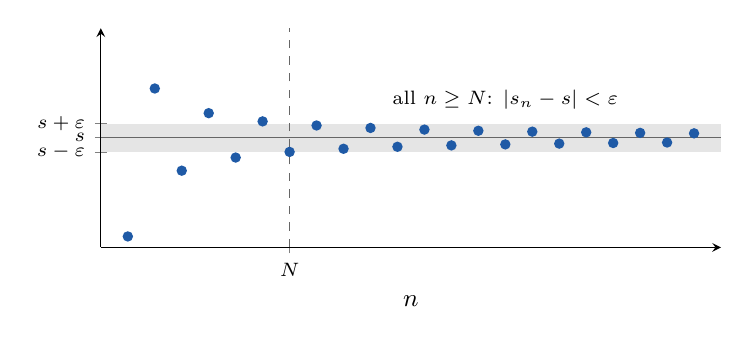
\begin{tikzpicture}
\begin{axis}[nfig, width=0.78\textwidth, height=0.36\textwidth,
  xmin=0, xmax=23, ymin=0, ymax=2.0,
  xtick={7}, xticklabels={$N$}, ytick={0.87,1,1.13},
  yticklabels={$s-\varepsilon$,$s$,$s+\varepsilon$}, xlabel={$n$}]
  \addplot[draw=none, fill=black!10] coordinates {(0,0.87) (23,0.87) (23,1.13) (0,1.13)};
  \addplot[black!60, thin] coordinates {(0,1) (23,1)};
  \draw[black!60, dashed] (axis cs:7,0) -- (axis cs:7,2.0);
  \addplot[only marks, mark=*, mark size=1.4pt, figB] coordinates {(1,0.1000) (2,1.4500) (3,0.7000) (4,1.2250) (5,0.8200) (6,1.1500) (7,0.8714) (8,1.1125) (9,0.9000) (10,1.0900) (11,0.9182) (12,1.0750) (13,0.9308) (14,1.0643) (15,0.9400) (16,1.0562) (17,0.9471) (18,1.0500) (19,0.9526) (20,1.0450) (21,0.9571) (22,1.0409)};
  \node[font=\scriptsize] at (axis cs:15,1.35) {all $n \geq N$: $|s_n - s| < \varepsilon$};
\end{axis}
\end{tikzpicture}\figcap{The $(\varepsilon, N)$ picture: however narrow the band $s \pm \varepsilon$, some stage $N$ exists beyond which every dot lies inside. Early terms may wander freely --- convergence is a statement about tails. (Compare \S 24: uniform convergence of functions is this same picture with dots replaced by whole graphs.)}
\end{center}


\begin{rembox}[What does the definition catch?]
The condition $|s_n - s| < \varepsilon$ says $s_n$ approximates $s$ with error less than $\varepsilon$. The definition demands: \emph{no matter how small an error tolerance $\varepsilon$ is prescribed, from some stage $N$ onward, every term of the sequence meets that tolerance.} The order of quantifiers is essential: $\varepsilon$ is given first (arbitrarily), and $N$ is allowed to depend on $\varepsilon$.
\end{rembox}

\begin{defbox}[Divergence]
If there exists no real number $s$ such that $(s_n)$ converges to $s$, we say $(s_n)$ \textbf{diverges}. For example, $s_n = 2^n$ diverges (it is unbounded; see \S 9).
\end{defbox}

\begin{exbox}[Constant sequence]
If $s_n = 1$ for all $n$, then $\lim_{n\to\infty} s_n = 1$. Checking the definition: given $\varepsilon > 0$, take $N = 1$; for every $n \geq N$, $|s_n - 1| = 0 < \varepsilon$. \hfill $\blacksquare$
\end{exbox}

\begin{exbox}[$1/n \to 0$]
If $s_n = \tfrac1n$ for $n \geq 1$, then $\lim_{n\to\infty} s_n = 0$.

\emph{Proof.} For $\varepsilon > 0$, we need to find $N$. Take $N$ such that $N > \tfrac{1}{\varepsilon}$ --- why can we do this? By the \emph{Archimedean Property} (\S 4). When $n \geq N$, we have $n > \tfrac1\varepsilon$, hence
\[
|s_n - 0| = \frac1n < \varepsilon. \tag*{$\blacksquare$}
\]
\end{exbox}

\begin{rembox}[How did we find $N$?]
Usually we \emph{solve the inequality} $|s_n - s| < \varepsilon$ for $n$. In the example above: we want $\tfrac1n < \varepsilon$, i.e.\ $n > \tfrac1\varepsilon$; so we take any positive integer $N > \tfrac1\varepsilon$. The same method handles $s_n = (-1)^n \tfrac1n$ (since $|s_n - 0| = \tfrac1n$, the same $N$ works) and $s_n = \tfrac{1}{n^2}$: solving $\tfrac{1}{n^2} < \varepsilon$ gives $n^2 > \tfrac1\varepsilon$, i.e.\ $n > \sqrt{1/\varepsilon}$, so take $N > \sqrt{1/\varepsilon}$. There are several valid choices of $N$ --- any sufficiently large one works.
\end{rembox}

\begin{exbox}[Simplifying before solving]
Let $s_n = \dfrac{n}{n+1}$. Prove $s_n \to 1$.

\emph{Proof.} Compute
\[
\left| \frac{n}{n+1} - 1 \right| = \left| \frac{n - 1 - n}{1+n} \right| = \frac{1}{1+n}.
\]
We could solve $\tfrac{1}{1+n} < \varepsilon$ directly, but we can also \emph{simplify first}:
\[
\frac{1}{1+n} < \frac1n,
\]
so it is good enough to have $\tfrac1n < \varepsilon$, and we can take $N > \tfrac1\varepsilon$. \hfill $\blacksquare$
\end{exbox}

\begin{exbox}[When the naive simplification fails]
Let $s_n = \dfrac{n}{n-1}$, $n \geq 2$. Prove $s_n \to 1$.

Here $\left| \tfrac{n}{n-1} - 1 \right| = \left| \tfrac{n - (n-1)}{n-1} \right| = \tfrac{1}{n-1}$. Can we simplify by replacing $\tfrac{1}{n-1}$ by $\tfrac1n$? \textbf{No:} $\tfrac{1}{n-1} > \tfrac1n$, so $\tfrac1n < \varepsilon$ does \emph{not} imply $\tfrac{1}{n-1} < \varepsilon$ --- an upper bound must be replaced by something \emph{larger}, not smaller. Two correct ways:
\begin{enumerate}[label=(\arabic*)]
    \item \emph{Directly:} $\tfrac{1}{n-1} < \varepsilon \iff n - 1 > \tfrac1\varepsilon \iff n > \tfrac1\varepsilon + 1$. Take $N > \tfrac1\varepsilon + 1$.
    \item \emph{Bound by a simpler expression:} for $n \geq 2$, $n - 1 \geq \tfrac{n}{2}$, so $\tfrac{1}{n-1} \leq \tfrac2n$. It suffices to have $\tfrac2n < \varepsilon$, i.e.\ $n > \tfrac2\varepsilon$. Take $N > \tfrac2\varepsilon$. \hfill $\blacksquare$
\end{enumerate}
\end{exbox}

\subsection{Uniqueness of the Limit}

The first property of limits --- and our first theorem with a real proof about them.

\begin{thmbox}[Uniqueness of Limits]
If a sequence $(s_n)$ has a limit, then the limit is unique: if $\lim_{n\to\infty} s_n = s$ and $\lim_{n\to\infty} s_n = t$, then $s = t$.
\end{thmbox}

\begin{proof}
Suppose not: $s \neq t$. Then $s - t \neq 0$, hence $|s - t| > 0$. We look for a contradiction.

Take $\varepsilon$ with $0 < \varepsilon < \tfrac12 |s - t|$. By the definition of $s_n \to s$, there exists $N_1$ such that $|s_n - s| < \varepsilon$ for $n \geq N_1$. Similarly, there exists $N_2$ such that $|s_n - t| < \varepsilon$ for $n \geq N_2$. Take $N = \max\{N_1, N_2\}$; then for $n \geq N$ \emph{both} inequalities hold. By the triangle inequality, for any such $n$,
\[
|s - t| = |(s - s_n) - (t - s_n)| \leq |s - s_n| + |t - s_n| < \varepsilon + \varepsilon = 2\varepsilon < |s - t|.
\]
So $|s - t| < |s - t|$ --- a contradiction. Where does it come from? From the assumption $s \neq t$, which gave $|s-t| > 0$ and allowed the choice of $\varepsilon$. Hence $s = t$.
\end{proof}

\begin{rembox}[Summary of the method]
To determine whether $(s_n)$ is convergent, we determine whether it has a limit, in two steps:
\begin{enumerate}[label=(\arabic*)]
    \item \textbf{guess} a limit $s$;
    \item \textbf{prove} it by the $(\varepsilon, N)$ definition --- the key point being to solve $N$ in terms of $\varepsilon$.
\end{enumerate}
\end{rembox}

% ============================================================================
% SECTION 8: A DISCUSSION ABOUT PROOFS
% ============================================================================

\section{A Discussion About Proofs}

This section is a workshop on the two-step method: guess the limit, then prove it. The recurring technique: simplify $|s_n - s|$ by replacing it with a \emph{simpler upper bound}, then solve $N$ in terms of $\varepsilon$ --- the point being to get a simple, clean formula for $N$.

\subsection{Guessing and Proving}

\begin{exbox}[An indeterminate form of type $\infty - \infty$]
Let $s_n = \sqrt{n^2 + n + 1} - n$. Determine whether it converges; if yes, guess the limit and prove it.

\textbf{Guessing.} The expression is of the type $\infty - \infty$; we need to get rid of the $\infty$'s. Multiply and divide by the conjugate:
\begin{align*}
\sqrt{n^2+n+1} - n
&= \frac{(\sqrt{n^2+n+1} + n)(\sqrt{n^2+n+1} - n)}{\sqrt{n^2+n+1} + n}\\
&= \frac{n^2 + n + 1 - n^2}{\sqrt{n^2+n+1} + n}
= \frac{n+1}{\sqrt{n^2+n+1} + n}.
\end{align*}
Then what? \emph{Look at the main term and ignore lower-order ones:}
\[
\approx \frac{n}{\sqrt{n^2} + n} = \frac{n}{n + n} = \frac12.
\]
So we guess $s_n \to \tfrac12$.

\textbf{Proving.} We compute $|s_n - \tfrac12|$ and simplify, again via the conjugate (now of $\sqrt{n^2+n+1} - (n + \tfrac12)$):
\[
\left| s_n - \tfrac12 \right|
= \left| \frac{n^2+n+1 - (n+\tfrac12)^2}{\sqrt{n^2+n+1} + n + \tfrac12} \right|
= \frac{\tfrac34}{\sqrt{n^2+n+1} + n + \tfrac12}
< \frac{\tfrac34}{n + n}
< \frac1n.
\]
(In the second-to-last step we threw away a lot --- using only $\sqrt{n^2+n+1} > n$ --- but an upper bound is all we need.) Now $\tfrac1n < \varepsilon$ suffices: take $N > \tfrac1\varepsilon$. \hfill $\blacksquare$
\end{exbox}

\begin{exbox}[Same method]
Let $s_n = \sqrt{9n^2 + n} - 3n$. By the conjugate trick,
\[
s_n = \frac{(\sqrt{9n^2+n} - 3n)(\sqrt{9n^2+n} + 3n)}{\sqrt{9n^2+n} + 3n}
= \frac{9n^2 + n - 9n^2}{\sqrt{9n^2+n} + 3n}
= \frac{n}{\sqrt{9n^2+n} + 3n}
\approx \frac{n}{3n + 3n} = \frac16,
\]
so the limit should be $\tfrac16$. \emph{Writing up the proof} (left as an exercise in lecture): from the display,
\begin{align*}
\left| s_n - \tfrac16 \right|
= \left| \frac{n}{\sqrt{9n^2+n} + 3n} - \frac16 \right|
&= \frac{\left| 6n - \sqrt{9n^2+n} - 3n \right|}{6\left(\sqrt{9n^2+n} + 3n\right)}\\
&= \frac{\left| 3n - \sqrt{9n^2+n} \right|}{6\left(\sqrt{9n^2+n} + 3n\right)}
= \frac{n}{6\left(\sqrt{9n^2+n} + 3n\right)^2},
\end{align*}
using the conjugate once more for $|3n - \sqrt{9n^2+n}| = \frac{n}{\sqrt{9n^2+n}+3n}$. Since $\sqrt{9n^2+n} + 3n > 6n$, the last quantity is $< \dfrac{n}{6 \cdot 36 n^2} < \dfrac1n$. So $N > \tfrac1\varepsilon$ works. \hfill $\blacksquare$
\end{exbox}

\subsection{Sequences Between $\mathbb{Q}$ and $\mathbb{R}$}

\begin{exbox}[Irrational terms with rational limit]
Give an example of a sequence of irrational numbers converging to a rational limit. Many choices --- for instance
\[
s_n = 1 + \frac{\pi}{n} \longrightarrow 1.
\]
Each $s_n$ is irrational (if $1 + \pi/n$ were rational, so would be $\pi$), and $|s_n - 1| = \pi/n < \varepsilon$ once $n > \pi/\varepsilon$.
\end{exbox}

\begin{exbox}[Rational terms with irrational limit]
Give an example of a sequence of rational numbers converging to an irrational limit --- say $s = \tfrac{\pi}{4}$.

Here we need an \emph{algorithm}, not a formula for $s_n$. Note $\tfrac\pi4 \in [0,1]$. Divide $[0,1]$ into two equal intervals $[0, \tfrac12]$, $[\tfrac12, 1]$, and keep the one containing $\tfrac\pi4$. Dividing again and again into halves, we get a nested sequence of intervals containing $\tfrac\pi4$, the $n$-th of length $\tfrac{1}{2^n}$, with rational endpoints. Take $s_n$ to be the left endpoint of the $n$-th interval. Then $s_n \in \mathbb{Q}$ and
\[
\left| s_n - \frac\pi4 \right| \leq \frac{1}{2^n} \longrightarrow 0,
\]
so $s_n \to \tfrac\pi4$. (Are there other solutions? Certainly --- e.g.\ truncated decimal expansions, once those are available.)
\end{exbox}

\subsection{Limits and Absolute Values; a Divergent Sequence}

\begin{exbox}[$s_n \to 0 \iff |s_n| \to 0$]
Prove: $\lim_{n\to\infty} s_n = 0$ if and only if $\lim_{n\to\infty} |s_n| = 0$.

\emph{Proof.} Compare the $(\varepsilon, N)$ conditions for the two statements. For the first: $|s_n - 0| = |s_n| < \varepsilon$. For the second: $\big| |s_n| - 0 \big| = \big| |s_n| \big| = |s_n| < \varepsilon$. The two conditions are \emph{identical}, so for any $\varepsilon$, the same $N$ witnesses both. \hfill $\blacksquare$
\end{exbox}

\begin{exbox}[$|s_n|$ converges but $s_n$ diverges]
Take $s_n = (-1)^n$. Then $|s_n| = 1$ clearly converges. But $(s_n)$ does not converge.

\emph{Proof.} Suppose it did, with $s = \lim_{n\to\infty} s_n$. Let $\varepsilon > 0$ be arbitrary; there exists $N$ such that $|s_n - s| < \varepsilon$ for all $n \geq N$. Choosing an \emph{even} $n \geq N$ (e.g.\ $n = 2N$), where $s_n = 1$, gives $|1 - s| < \varepsilon$. Since $\varepsilon > 0$ was arbitrary, $|1 - s| = 0$, i.e.\ $s = 1$. Choosing an \emph{odd} $n \geq N$ (e.g.\ $n = 2N+1$), where $s_n = -1$, gives $|-1 - s| = |1 + s| < \varepsilon$, and by the same argument $s = -1$. So $s = 1$ and $s = -1$ --- impossible. Hence $(s_n)$ diverges. (The book has a different proof.) \hfill $\blacksquare$
\end{exbox}

\subsection{The Squeeze Theorem}

\begin{thmbox}[Squeeze Theorem]
Given three sequences $(a_n), (b_n), (c_n)$ satisfying
\[
a_n \leq b_n \leq c_n \quad \text{for all } n,
\]
assume $\lim_{n\to\infty} a_n = \lim_{n\to\infty} c_n = s$. Then $(b_n)$ also converges to $s$.
\end{thmbox}

\begin{proof}
The idea: $|a_n - s| < \varepsilon$ if and only if $-\varepsilon < a_n - s < \varepsilon$, equivalently
\[
s - \varepsilon < a_n < s + \varepsilon,
\]
and the same unpacking applies to $c_n$ and $b_n$.

Given $\varepsilon > 0$: since $a_n \to s$, there is $N_1$ with $s - \varepsilon < a_n < s + \varepsilon$ for $n \geq N_1$; since $c_n \to s$, there is $N_2$ with $s - \varepsilon < c_n < s + \varepsilon$ for $n \geq N_2$. Take $N = \max\{N_1, N_2\}$. For $n \geq N$, using the sandwich hypothesis,
\[
s - \varepsilon < a_n \leq b_n \leq c_n < s + \varepsilon,
\]
so $|b_n - s| < \varepsilon$. Hence $b_n \to s$.
\end{proof}

\begin{exbox}[Null sequence times bounded sequence]
First: if $s_n \to 0$, then for any number $M$, also $M s_n \to 0$. (By definition: given $\varepsilon > 0$, if $M = 0$ there is nothing to prove; otherwise choose $N$ with $|s_n| < \varepsilon / |M|$ for $n \geq N$; then $|M s_n| < \varepsilon$.)

Now, by the Squeeze Theorem and this observation: \emph{if $s_n \to 0$ and $(t_n)$ is a bounded sequence --- i.e.\ there exists $M > 0$ such that $|t_n| \leq M$ for all $n$ --- then $s_n t_n \to 0$.}

\emph{Proof.} Just note
\[
-|s_n| M \leq s_n t_n \leq |s_n| M,
\]
and the fact that $|s_n| \to 0$ too (previous subsection). Hence both outer sequences $-|s_n|M$ and $|s_n|M$ converge to $0$, and the middle sequence $s_n t_n$ converges to $0$ by squeezing. \hfill $\blacksquare$
\end{exbox}

\subsection{Two More Worked Examples}

\begin{exbox}[Square roots preserve limits]
Let $(s_n)$ be a sequence of nonnegative numbers with $s = \lim_{n\to\infty} s_n \geq 0$. Prove $\sqrt{s_n} \to \sqrt{s}$.

What is known? That $|s_n - s|$ is small. So we must bound $|\sqrt{s_n} - \sqrt{s}|$ from above \emph{in terms of} $|s_n - s|$, getting rid of the square roots --- by the conjugate again:
\[
\left| \sqrt{s_n} - \sqrt{s} \right|
= \left| \frac{(\sqrt{s_n} + \sqrt{s})(\sqrt{s_n} - \sqrt{s})}{\sqrt{s_n} + \sqrt{s}} \right|
= \frac{|s_n - s|}{\sqrt{s_n} + \sqrt{s}}.
\]
It is good that $s_n - s$ appears in the numerator. How about the denominator?

\textbf{Case $s > 0$.} Then $\sqrt{s_n} + \sqrt{s} \geq \sqrt{s}$, so
\[
\left| \sqrt{s_n} - \sqrt{s} \right| \leq \frac{|s_n - s|}{\sqrt{s}}.
\]
Write-up: given $\varepsilon > 0$, take $N$ such that $|s_n - s| < \sqrt{s}\, \varepsilon$ for $n \geq N$ (possible since $s_n \to s$). Then for $n \geq N$, $|\sqrt{s_n} - \sqrt{s}| < \varepsilon$.

\textbf{Is this the end of the proof? No} --- the bound divided by $\sqrt{s}$, so the case $s = 0$ needs separate treatment.

\textbf{Case $s = 0$.} We want $|\sqrt{s_n}| < \varepsilon$, which is equivalent to $|s_n| < \varepsilon^2$. The latter is achievable since $s_n \to 0$: given $\varepsilon > 0$, apply the definition of $s_n \to 0$ with the tolerance $\varepsilon^2 > 0$ to get $N$ such that $|s_n| < \varepsilon^2$ for $n \geq N$; then $|\sqrt{s_n} - 0| < \varepsilon$ for $n \geq N$. So $\sqrt{s_n} \to 0$. \hfill $\blacksquare$
\end{exbox}

\begin{exbox}[Eventually above $a$]
Assume $(s_n)$ is convergent with $\lim_{n\to\infty} s_n = s > a$. Prove there exists $N$ such that $s_n > a$ for all $n \geq N$.

\emph{Finding the proof.} For any $\varepsilon$, when $n$ is large, $|s_n - s| < \varepsilon$, i.e.
\[
s - \varepsilon < s_n < s + \varepsilon.
\]
We want $s - \varepsilon > a$, i.e.\ $\varepsilon < s - a$ --- which is a legitimate choice since $s - a > 0$.

\emph{Write-up.} Set $\varepsilon = s - a > 0$. There exists $N$ such that $|s_n - s| < \varepsilon$ for $n \geq N$. Then for such $n$,
\[
s_n > s - \varepsilon = s - (s - a) = a. \tag*{$\blacksquare$}
\]
\end{exbox}

% ============================================================================
% SECTION 9: LIMIT THEOREMS FOR SEQUENCES
% ============================================================================

\section{Limit Theorems for Sequences}

We want to simplify life --- not using $(\varepsilon, N)$ every time. The theorems of this section let us compute limits by combining known ones.

\subsection{Convergent Implies Bounded}

\begin{thmbox}[Convergent Sequences Are Bounded]
If a sequence $(s_n)_{n=1}^{\infty}$ is convergent, then it is \textbf{bounded}: there exists a number $M$ such that $|s_n| \leq M$ for all $n \geq 1$, i.e.\ the set $\{|s_n| \mid n \in \mathbb{N}\}$ is bounded.
\end{thmbox}

\begin{proof}
Let $s = \lim_{n\to\infty} s_n$. Take $\varepsilon = 1$ in the definition: there exists $N$ such that $|s_n - s| < 1$ for all $n \geq N$. By the triangle inequality, for such $n$,
\[
|s_n| = |(s_n - s) + s| \leq |s_n - s| + |s| < |s| + 1.
\]
\textbf{Can we take $M = |s| + 1$? No} --- don't forget the finitely many initial terms $s_1, \ldots, s_N$, which the bound above says nothing about. So take
\[
M = \max\{|s_1|, \ldots, |s_N|,\ |s| + 1\},
\]
a maximum of a \emph{finite} set (which exists, \S 4). Now $|s_n| \leq M$ for all $n \geq 1$.
\end{proof}

\begin{exbox}[$\sqrt{n}$ diverges]
The sequence $s_n = \sqrt{n}$ is not convergent. Why? It is unbounded: given any $M$, the Archimedean property provides $n > M^2$, and then $\sqrt{n} > M$. By the contrapositive of the theorem, an unbounded sequence cannot converge.
\end{exbox}

\subsection{Arithmetic of Limits}

\begin{thmbox}[Scalar Multiples]
If $(s_n)$ is convergent, then for any $k \in \mathbb{R}$, $(k s_n)$ is also convergent, and
\[
\lim_{n\to\infty} k s_n = k \lim_{n\to\infty} s_n
\]
--- the limit and the multiplication can be exchanged.
\end{thmbox}

\begin{proof}
Let $s = \lim s_n$. If $k = 0$ the sequence is constantly $0$. Otherwise, given $\varepsilon > 0$, choose $N$ with $|s_n - s| < \varepsilon / |k|$ for $n \geq N$; then $|k s_n - k s| = |k| \, |s_n - s| < \varepsilon$.
\end{proof}

\begin{thmbox}[Sums and Products]
If $s_n \to s$ and $t_n \to t$, then
\[
s_n + t_n \to s + t \qquad \text{and} \qquad s_n t_n \to s t.
\]
\end{thmbox}

\begin{proof}
\textbf{Sum} (the easy one). Given $\varepsilon > 0$, we can require
\[
|s_n - s| < \frac\varepsilon2 \quad (n \geq N_1) \qquad \text{and} \qquad |t_n - t| < \frac\varepsilon2 \quad (n \geq N_2),
\]
by applying the definitions with tolerance $\varepsilon/2$. For $n \geq N = \max\{N_1, N_2\}$, the triangle inequality gives
\[
|s_n + t_n - (s + t)| \leq |s_n - s| + |t_n - t| < \frac\varepsilon2 + \frac\varepsilon2 = \varepsilon.
\]

\textbf{Product.} What is $|s_n t_n - st|$? Add and subtract the mixed term $s t_n$:
\[
|s_n t_n - s t| = |s_n t_n - s t_n + s t_n - s t|
\leq |s_n t_n - s t_n| + |s t_n - s t|
= |s_n - s|\,|t_n| + |t_n - t|\,|s|.
\]
If both summands are $< \varepsilon/2$, we are done. How? Since $(t_n)$ is convergent, it is \emph{bounded} (Theorem 9.1): there exists $M > 0$ with $|t_n| \leq M$ for all $n$; enlarging $M$ if necessary, we may also assume $|s| \leq M$. Then
\[
|s_n - s|\,|t_n| \leq M |s_n - s|, \qquad |t_n - t|\,|s| \leq M |t_n - t|.
\]
Now, given $\varepsilon > 0$, require
\[
M |s_n - s| < \frac\varepsilon2 \quad (n \geq N_1) \qquad \text{and} \qquad M |t_n - t| < \frac\varepsilon2 \quad (n \geq N_2),
\]
i.e.\ apply the two convergence definitions with tolerance $\varepsilon / (2M)$. For $n \geq \max\{N_1, N_2\}$,
\[
|s_n t_n - st| \leq M|s_n - s| + M|t_n - t| < \varepsilon. \qedhere
\]
\end{proof}

\textbf{What is next? Division!}

\begin{thmbox}[Quotients]
Assume $s_n \to s$ and $t_n \to t$, with $t \neq 0$ (and $t_n \neq 0$ for all $n$, so the quotients are defined). Then
\[
\frac{s_n}{t_n} \longrightarrow \frac{s}{t}.
\]
\end{thmbox}

\begin{proof}
The idea is the same. Combine over a common denominator and insert the mixed term $st$:
\[
\left| \frac{s_n}{t_n} - \frac{s}{t} \right|
= \left| \frac{s_n t - s t_n}{t_n t} \right|
= \left| \frac{s_n t - st + st - s t_n}{t_n t} \right|
\leq \frac{|s_n - s|\,|t| + |s|\,|t - t_n|}{|t_n|\,|t|}.
\]
The new issue is the denominator: we need $|t_n|$ bounded away from $0$. Since $|t_n| \to |t| > \tfrac{|t|}{2}$, the ``eventually above $a$'' example of \S 8 (applied to the sequence $|t_n|$ with $a = |t|/2$) gives $N_0$ such that
\[
|t_n| > \frac{|t|}{2} \qquad \text{for } n \geq N_0.
\]
For such $n$,
\[
\left| \frac{s_n}{t_n} - \frac{s}{t} \right|
\leq \frac{|s_n - s|\,|t| + |s|\,|t_n - t|}{\tfrac{|t|}{2}\,|t|}
= \frac{2}{|t|} |s_n - s| + \frac{2|s|}{|t|^2} |t_n - t|.
\]
Both coefficients are fixed constants, so as in the product proof: given $\varepsilon > 0$, choose $N_1$ with $\tfrac{2}{|t|}|s_n - s| < \tfrac\varepsilon2$ for $n \geq N_1$, and $N_2$ with $\tfrac{2|s|}{|t|^2}|t_n - t| < \tfrac\varepsilon2$ for $n \geq N_2$ (if $s = 0$ the second term vanishes and any $N_2$ works). For $n \geq \max\{N_0, N_1, N_2\}$, the sum is $< \varepsilon$.
\end{proof}

An order-theoretic companion to the arithmetic rules --- invoked constantly in these notes as ``limits preserve $\leq$'':

\begin{propbox}[Limits Preserve Weak Inequalities (HW)]
Suppose there exists $N_0$ such that $s_n \leq t_n$ for all $n > N_0$, and suppose $\lim s_n = s$ and $\lim t_n = t$ exist. Then
\[
s \leq t.
\]
\end{propbox}

\begin{proof}
Assume for contradiction $s > t$, and set $\varepsilon = \tfrac{s-t}{2} > 0$. By the difference rule, $t_n - s_n \to t - s$, so there is $N_1$ such that for $n > N_1$,
\[
|(t_n - s_n) - (t - s)| < \varepsilon, \qquad \text{in particular} \qquad t_n - s_n < (t - s) + \frac{s-t}{2} = \frac{t-s}{2} < 0.
\]
But for $n > \max\{N_0, N_1\}$ the hypothesis gives $t_n - s_n \geq 0$ --- contradiction. Hence $s \leq t$.
\end{proof}

\begin{rembox}
\emph{Strict} inequalities are \textbf{not} preserved: $0 < \tfrac1n$ for every $n$, yet both limits equal $0$. Passing to the limit can only be trusted with $\leq$.
\end{rembox}

\subsection{Basic Sequences}

To apply the theorems, we need a stock of basic limits.

\begin{exbox}[$1/n^p \to 0$ for $p > 0$]
By the $(\varepsilon, N)$ definition: $\tfrac{1}{n^p} < \varepsilon$ if and only if $n^p > \tfrac1\varepsilon$, i.e.\ $n > (1/\varepsilon)^{1/p}$; take $N > (1/\varepsilon)^{1/p}$. \hfill $\blacksquare$
\end{exbox}

\begin{exbox}[$a^n \to 0$ for $0 < a < 1$]
There are several proofs. \emph{The lecture's proof, via logarithms:} we want $|a^n| = a^n < \varepsilon$. Taking $\log$ --- legitimate for comparing since $\log$ is an increasing function --- gives $n \log a < \log \varepsilon$. Since $\log a < 0$, dividing \emph{flips} the inequality:
\[
n > \frac{\log \varepsilon}{\log a},
\]
so take $N > \tfrac{\log\varepsilon}{\log a}$. \hfill $\blacksquare$
\end{exbox}

\begin{rembox}
Strictly speaking, the logarithm has not yet been rigorously defined in this course --- like the decimal expansion in \S 4, it is borrowed from the future. A proof from what we have: write $\tfrac1a = 1 + b$ with $b > 0$. By the binomial formula (below), $(1+b)^n \geq 1 + nb > nb$, so
\[
0 < a^n = \frac{1}{(1+b)^n} < \frac{1}{nb} \longrightarrow 0,
\]
and $a^n \to 0$ by the Squeeze Theorem.
\end{rembox}

\begin{exbox}[$n^{1/n} \to 1$]
Define $s_n = n^{1/n} - 1$; the claim is equivalent to $s_n \to 0$. Note $s_n \geq 0$ for $n \geq 1$, and
\[
1 + s_n = n^{1/n}, \qquad \text{so raising to the power } n: \qquad (1 + s_n)^n = n.
\]
Now recall the \textbf{binomial formula}:
\[
(a+b)^n = a^n + n a^{n-1} b + \frac12 n(n-1) a^{n-2} b^2 + \cdots + n a b^{n-1} + b^n.
\]
If $a > 0$ and $b \geq 0$, all terms are nonnegative, so keeping only one term,
\[
(a+b)^n \geq \frac12 n(n-1) a^{n-2} b^2.
\]
Applying this with $a = 1$, $b = s_n$:
\[
n = (1 + s_n)^n \geq \frac12 n(n-1) s_n^2,
\]
hence for $n \geq 2$,
\[
s_n^2 \leq \frac{2}{n-1}, \qquad \text{i.e.} \qquad 0 \leq s_n \leq \sqrt{\frac{2}{n-1}}.
\]
Is it clear now that $s_n \to 0$? Yes, by the \emph{Squeeze Theorem}: $\tfrac{2}{n-1} \to 0$ (e.g.\ $\tfrac{2}{n-1} \leq \tfrac4n$ for $n \geq 2$), hence $\sqrt{2/(n-1)} \to 0$ by the square-root example of \S 8, and $s_n$ is squeezed between $0$ and a null sequence. \hfill $\blacksquare$
\end{exbox}

\begin{corbox}[Linear Combinations]
If $s_n \to s$ and $t_n \to t$, then for any two constants $a, b$,
\[
a s_n + b t_n \longrightarrow a s + b t.
\]
(Combine the scalar-multiple and sum theorems.) So the limit commutes with \emph{linear combinations} --- a very important concept in linear algebra --- and, with products and quotients, with all the basic arithmetic operations.
\end{corbox}

\begin{exbox}[$a^{1/n} \to 1$ for any $a > 0$]
Why is this true? First observe the pattern experimentally. If $a \geq 1$: $a^{1/2} \geq 1$ but smaller than $a$; $a^{1/3} \geq 1$ but smaller than $a^{1/2}$ --- the sequence decreases toward $1$ from above. If $a \leq 1$, symmetrically, it increases toward $1$ from below.

\emph{Proof.} \textbf{Case (i): $a \geq 1$.} When $n > a$ (Archimedean), $a^{1/n} < n^{1/n}$; and clearly $1 \leq a^{1/n}$. So we have the squeezing
\[
1 \leq a^{1/n} < n^{1/n}.
\]
Both outer sequences ($s_n = 1$ and $t_n = n^{1/n}$) converge to $1$, so $a^{1/n} \to 1$ by the Squeeze Theorem.

\textbf{Case (ii): $a < 1$.} Then $\tfrac1a > 1$, and by case (i) together with the quotient limit theorem,
\[
a^{1/n} = \frac{1}{(1/a)^{1/n}} \longrightarrow \frac11 = 1. \tag*{$\blacksquare$}
\]
\end{exbox}

\begin{exbox}[Finding the limit of a recursion]
Let $t_1 = 1$ and $t_{n+1} = \dfrac{t_n^2 + 2}{2 t_n}$. \emph{Assuming} $(t_n)$ is convergent, find $t = \lim_{n\to\infty} t_n$.

Rewrite the recursion as $t_{n+1} \cdot (2 t_n) = t_n^2 + 2$. Both sides are convergent sequences ($\lim t_{n+1} = \lim t_n = t$, as the shifted sequence has the same limit), so applying the product and sum limit theorems,
\[
2 t^2 = t^2 + 2, \qquad \text{i.e.} \qquad t^2 = 2.
\]
Since $t_1 = 1 > 0$ and the recursion preserves positivity (by induction), $t \geq 0$; hence $t = \sqrt2$. (This recursion is exactly Newton's method for solving $x^2 = 2$.)
\end{exbox}

\begin{exbox}[Limit theorems prove non-existence too]
Let $x_1 = 1$ and $x_{n+1} = 3 x_n^2$ for $n \geq 1$.

\textbf{(a)} If $a = \lim x_n$ exists, prove $a = \tfrac13$ or $a = 0$. Note $\lim x_{n+1} = \lim x_n = a$; taking limits in the recursion (product theorem) gives
\[
a = 3a^2, \qquad \text{i.e.} \qquad a(3a - 1) = 0.
\]

\textbf{(b)} Does $\lim x_n$ exist? \textbf{No!} Why: $x_1 = 1$ and $x_2 = 3 > 1$; by induction, if $x_n \geq 1$ then $x_{n+1} = 3x_n^2 \geq 3 > 1$, so $x_n \geq 1$ for all $n$. If the limit existed it would satisfy $a \geq 1$ (limits preserve $\geq$), contradicting (a). So the two candidate values rule each other out --- the sequence diverges. \hfill $\blacksquare$
\end{exbox}

\subsection{Divergence to $\pm\infty$}

Earlier we introduced the extended real numbers $[-\infty, +\infty]$ (\S 5). We now define the related notions $x_n \to +\infty$ and $x_n \to -\infty$. Compare two examples: $s_n = n$ and $t_n = (-1)^n n$. Both are divergent (both are unbounded --- Theorem 9.1). But there is a difference: $s_n$ still has \emph{some} convergence behavior --- it goes steadily up --- while $t_n$ jumps between $\pm\infty$ directions.

\begin{defbox}[Divergence to Infinity]
We say $s_n$ \textbf{diverges to $+\infty$}, written $s_n \to +\infty$ or $\lim_{n\to\infty} s_n = +\infty$, if for any positive number $M$ (usually large), there exists $N$ such that for all $n > N$,
\[
s_n > M.
\]
Similarly, $s_n \to -\infty$ if for any $M$ there exists $N$ such that $s_n < -M$ for all $n > N$.
\end{defbox}

\begin{exbox}[Basic examples]
$s_n = n^2 \to +\infty$ and $s_n = 3^{n-1} \to +\infty$ (given $M$, take $N > \sqrt{M}$, resp.\ use $3^{n-1} \geq n$ for $n \geq 1$, provable by induction). Meanwhile $t_n = (-1)^n n$ diverges but tends to neither $+\infty$ nor $-\infty$.
\end{exbox}

\begin{lembox}[Squeezing to Infinity]
If $s_n \to +\infty$ and $t_n \geq s_n$ for all $n$, then $t_n \to +\infty$.
\end{lembox}

\begin{proof}
Given $M$, take $N$ with $s_n > M$ for $n > N$; then $t_n \geq s_n > M$ for $n > N$. (The same proof gives the \emph{eventual} version: it suffices that $t_n \geq s_n$ for $n > N_0$ --- replace $N$ by $\max\{N, N_0\}$. Similarly, $t_n \to -\infty$ and $s_n \leq t_n$ eventually force $s_n \to -\infty$. Both refinements were HW.)
\end{proof}

\begin{propbox}[Adding a Sequence Bounded Below (HW)]
If $s_n \to +\infty$ and $\inf\{t_n \mid n \in \mathbb{N}\} > -\infty$, then
\[
s_n + t_n \to +\infty.
\]
In particular, the conclusion holds whenever $(t_n)$ is bounded, or convergent, or $t_n \to +\infty$.
\end{propbox}

\begin{proof}
Let $t_0 = \inf\{t_n\} \in \mathbb{R}$, so $t_n \geq t_0$ for all $n$. Given $M > 0$: since $s_n \to +\infty$, there is $N$ with $s_n > M - t_0$ for all $n > N$. Then for such $n$,
\[
s_n + t_n \geq s_n + t_0 > (M - t_0) + t_0 = M.
\]
For the particular cases, only $\inf t_n > -\infty$ must be checked: a bounded sequence satisfies it directly; a convergent one is bounded (\S 9); and if $t_n \to +\infty$, then all but finitely many terms exceed $0$, and a finite set of terms is bounded. (Compare the forbidden $(+\infty) - (+\infty)$ of \S 5: a lower bound on the perturbation is exactly what rules the bad case out.)
\end{proof}

\begin{exbox}[The recursion again]
The sequence $x_1 = 1$, $x_{n+1} = 3 x_n^2$ diverges to $+\infty$. Compute: $x_2 = 3$, $x_3 = 3 x_2^2 = 27 > 3^2$. \emph{Claim:} $x_n \geq 3^{n-1}$, by induction: true for $n = 1$; if $x_n \geq 3^{n-1}$, then
\[
x_{n+1} = 3 x_n^2 \geq 3 \cdot 3^{2n-2} = 3^{2n-1} \geq 3^n.
\]
Therefore $x_n \to +\infty$ by the squeezing lemma, since $3^{n-1} \to +\infty$. \hfill $\blacksquare$
\end{exbox}

\begin{exbox}[Complete classification of the geometric sequence]
For any $a \in \mathbb{R}$:
\begin{enumerate}[label=(\arabic*)]
    \item if $|a| < 1$, then $\lim_{n\to\infty} a^n = 0$;
    \item if $a = 1$, then $\lim_{n\to\infty} a^n = 1$;
    \item if $a > 1$, then $a^n \to +\infty$;
    \item if $a \leq -1$, then $\lim_{n\to\infty} a^n$ does not exist (not even as $\pm\infty$).
\end{enumerate}
\emph{Proofs.} (2) is clear. (1) By the Squeeze Theorem: $-|a|^n \leq a^n \leq |a|^n$, and $|a|^n \to 0$ (proved in the previous subsection), hence $-|a|^n \to 0$ too. (3) Check by definition: write $a = 1 + b$, $b > 0$; then $a^n \geq 1 + nb > nb \to +\infty$, and apply the squeezing lemma. (4) For $a = -1$ this is the example of \S 8. For $a < -1$: the terms satisfy $|a^n| = |a|^n \geq 1$ and alternate in sign, so by the same even/odd-subsequence argument as for $(-1)^n$, no finite limit exists; and neither $a^n \to +\infty$ nor $a^n \to -\infty$, since arbitrarily late terms are negative (resp.\ positive). \hfill $\blacksquare$
\end{exbox}

\subsection{The Ratio Test}

A simple criterion for convergence and divergence:

\begin{thmbox}[Ratio Test]
Assume $s_n \neq 0$ for all $n$ and that the limit $L = \displaystyle\lim_{n\to+\infty} \left| \frac{s_{n+1}}{s_n} \right|$ exists.
\begin{enumerate}[label=(\alph*)]
    \item If $L < 1$, then $\lim s_n = 0$.
    \item If $L > 1$, then $\lim |s_n| = +\infty$, and hence $(s_n)$ is divergent.
\end{enumerate}
\end{thmbox}

\begin{proof}
(a) Pick $\varepsilon > 0$ such that $L + \varepsilon < 1$ (possible since $L < 1$). By assumption, there exists $N$ such that for $n \geq N$,
\[
\left| \left| \frac{s_{n+1}}{s_n} \right| - L \right| < \varepsilon, \qquad \text{which implies} \qquad \left| \frac{s_{n+1}}{s_n} \right| < L + \varepsilon.
\]
Let $a = L + \varepsilon$, so $0 < a < 1$ and
\[
|s_{n+1}| < a |s_n| \qquad \text{for all } n \geq N.
\]
By induction this gives, for all $n > N$,
\[
|s_n| < a^{n - N} |s_N|
\]
(base case $n = N+1$ is the display; the step multiplies by one more factor of $a$). Now $a^{n-N} |s_N| = (a^{-N} |s_N|) \, a^n \to 0$ since $0 < a < 1$, so $|s_n| \to 0$ by squeezing, and hence $s_n \to 0$ (\S 8).

(b) Pick $\varepsilon > 0$ with $L - \varepsilon > 1$. By the same argument there exists $N$ such that $\left| \tfrac{s_{n+1}}{s_n} \right| > L - \varepsilon$ for $n \geq N$. Let $b = L - \varepsilon > 1$; then $|s_{n+1}| > b |s_n|$ for $n \geq N$, and by induction
\[
|s_n| > b^{n-N} |s_N| \qquad \text{for } n > N.
\]
Since $b > 1$ and $|s_N| > 0$, the right side tends to $+\infty$ (classification (3) above, scaled), so $|s_n| \to +\infty$ by the squeezing lemma. An unbounded sequence diverges.
\end{proof}

\begin{exbox}[Powers versus exponentials]
Let $a \in \mathbb{R}$ and $p \in \mathbb{R}$. Then:
\begin{enumerate}[label=(\arabic*)]
    \item if $|a| < 1$: $\lim_{n\to\infty} \dfrac{a^n}{n^p} = 0$;
    \item if $a > 1$: $\dfrac{a^n}{n^p} \to +\infty$;
    \item if $a < -1$: $\lim_{n\to\infty} \dfrac{a^n}{n^p}$ does not exist.
\end{enumerate}
For (1): if $p \geq 0$, compare $|a^n / n^p| \leq |a|^n \to 0$; if $p < 0$, apply the ratio test:
\[
\left| \frac{s_{n+1}}{s_n} \right| = |a| \left( \frac{n}{n+1} \right)^p \longrightarrow |a| < 1.
\]
For (2), the same ratio computation gives $L = a > 1$. For (3), the magnitudes $|a|^n / n^p \to +\infty$ by (2) while signs alternate. \hfill $\blacksquare$
\end{exbox}

\begin{exbox}[Factorials beat exponentials]
For all $a \in \mathbb{R}$: $\displaystyle\lim_{n\to\infty} \frac{a^n}{n!} = 0$. Use the ratio test (for $a \neq 0$):
\[
\left| \frac{s_{n+1}}{s_n} \right| = \frac{|a|^{n+1}/(n+1)!}{|a|^n/n!} = \frac{|a|}{n+1} \longrightarrow 0 = L < 1. \tag*{$\blacksquare$}
\]
\end{exbox}

\begin{rembox}[A scale of growth rates]
We have met different rates of growth, each of a strictly higher order than the previous:
\[
\underbrace{n^p \ (p > 0)}_{\text{power}} \quad \ll \quad \underbrace{a^n \ (a > 1)}_{\text{exponential}} \quad \ll \quad \underbrace{n!}_{\text{super-exponential}},
\]
where $\ll$ means the ratio of the earlier to the later tends to $0$ --- exactly the content of the two examples above (with the important special cases $2^n$ and $e^n$). Is there something $\to +\infty$ but \emph{slower than any power}? Answer: $s_n = \log n$. The lecture's argument that $\tfrac{\log n}{n} \to 0$: the ratio test does not work here; instead \emph{change variables}, $t = \log n$, so $n = e^t$ and
\[
\frac{\log n}{n} = \frac{t}{e^t} \longrightarrow 0 \quad \text{as } t \to +\infty,
\]
since the exponential grows at a higher rate than the power $t$. (As with $\log$ in the earlier example, this argument borrows the functions $\log$ and $e^t$ --- and limits along a continuous variable --- before their rigorous development; the honest statement is that it will become fully rigorous once those tools are available.)
\end{rembox}

% ============================================================================
% SECTION 10: MONOTONE SEQUENCES AND CAUCHY SEQUENCES
% ============================================================================

\section{Monotone Sequences and Cauchy Sequences}

So far, mainly three ways to determine whether a sequence converges: (1) guess the limit and check the $(\varepsilon, N)$ definition; (2) use basic examples plus the limit theorems and the Squeeze Theorem; (3) sometimes, the ratio test. But we need criteria that work \emph{without knowing the value of the limit} --- sometimes we need the existence of $\lim s_n$ even when we cannot compute it. In one important case, we can do it.

\subsection{Monotone Sequences}

\begin{defbox}[Monotone Sequences]
A sequence $(s_n)$ is called \textbf{increasing} if $s_n \leq s_{n+1}$ for all $n$, and \textbf{decreasing} if $s_n \geq s_{n+1}$ for all $n$. It is called \textbf{monotone} if it is either increasing or decreasing (the term includes both).
\end{defbox}

\begin{exbox}[Monotone or not]
(1) $s_n = n$ and $s_n = n^2$ are increasing. (2) $s_n = 1 - \tfrac1n$ is also increasing. (3) $s_n = 1 + (-1)^n \tfrac{1}{n^2}$ is \emph{not} monotone --- consecutive differences alternate in sign.

What is the difference between (1) and (2)? (1) is increasing but \emph{not bounded above} --- and not convergent. (2) is increasing \emph{and bounded} --- and converges to $1$.
\end{exbox}

\begin{thmbox}[Monotone Convergence Theorem]
If a sequence $(s_n)$ is monotone and bounded, then it is convergent.
\end{thmbox}

\begin{rembox}
Both assumptions are needed. Is there a bounded sequence that is not convergent? Yes: $s_n = (-1)^n$ --- the monotone condition is missing. And $s_n = n$ is monotone but unbounded.
\end{rembox}

\begin{proof}
Assume $(s_n)$ is increasing; the decreasing case is the same (using $\inf$ in place of $\sup$).

\emph{What can we take as the limit $s$?} Since $s_n \leq s_{n+1} \leq \cdots$, the limit should be $\geq$ every $s_n$ --- an upper bound of all the terms. And since the limit is unique, we do not want just \emph{any} upper bound; the natural candidate is the \emph{least} upper bound, which is unique.

Define the set $S = \{s_n \mid n \geq 1\}$. It is bounded (that is exactly the boundedness assumption on the sequence), and nonempty. By the \textbf{completeness axiom}, $s = \sup S$ exists and is a finite real number. We prove $s_n \to s$ by the $(\varepsilon, N)$ definition.

For any $\varepsilon > 0$: since $s - \varepsilon < s$, the number $s - \varepsilon$ is \emph{not} an upper bound of $S$ (characterization of the supremum, \S 4). Therefore there exists some element $s_N \in S$ with
\[
s_N > s - \varepsilon.
\]
Since $(s_n)$ is increasing, for any $n \geq N$ we have $s_n \geq s_N > s - \varepsilon$. Clearly also $s_n \leq s < s + \varepsilon$ ($s$ is an upper bound). So for all $n \geq N$,
\[
s - \varepsilon < s_n < s + \varepsilon, \qquad \text{i.e.} \qquad |s_n - s| < \varepsilon. \qedhere
\]
\end{proof}

\begin{center}
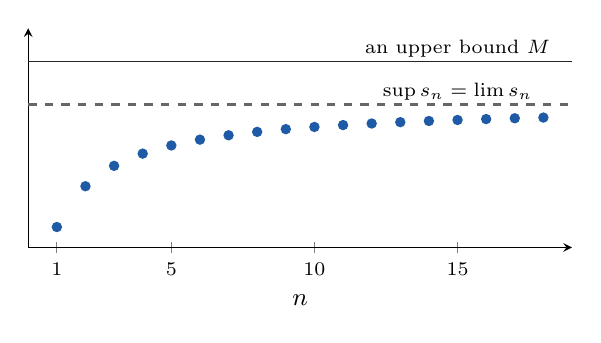
\begin{tikzpicture}
\begin{axis}[nfig, width=0.70\textwidth, height=0.36\textwidth,
  xmin=0, xmax=19, ymin=0.6, ymax=2.75,
  xtick={1,5,10,15}, ytick=\empty, xlabel={$n$}]
  \addplot[black!60, dashed] coordinates {(0,2) (19,2)};
  \addplot[black!85, thin] coordinates {(0,2.42) (19,2.42)};
  \addplot[only marks, mark=*, mark size=1.4pt, figB] coordinates {(1,0.8000) (2,1.2000) (3,1.4000) (4,1.5200) (5,1.6000) (6,1.6571) (7,1.7000) (8,1.7333) (9,1.7600) (10,1.7818) (11,1.8000) (12,1.8154) (13,1.8286) (14,1.8400) (15,1.8500) (16,1.8588) (17,1.8667) (18,1.8737)};
  \node[font=\scriptsize] at (axis cs:15.0,2.13) {$\sup s_n = \lim s_n$};
  \node[font=\scriptsize] at (axis cs:15.0,2.55) {an upper bound $M$};
\end{axis}
\end{tikzpicture}\figcap{The proof in one picture: an increasing sequence bounded above climbs toward the supremum of its own terms --- and converges exactly there. Any upper bound $M$ sits at or above the dashed line; the supremum is the least one.}
\end{center}


The supremum also admits a \emph{sequential} characterization --- the limit-language form of the approximation property of \S 4, and the engine inside several later proofs (e.g.\ the Extreme Value Theorem, \S 18):

\begin{propbox}[Sequential Characterization of the Supremum (HW)]
Let $S \subseteq \mathbb{R}$ be nonempty and bounded above. Then there exists a sequence $(s_n)$ of points of $S$ with
\[
\lim_{n\to\infty} s_n = \sup S.
\]
If moreover $\sup S \notin S$, the sequence can be chosen with $s_n < \sup S$ strictly for every $n$. In every case, the sequence can be chosen \emph{increasing}.
\end{propbox}

\begin{proof}
Write $s = \sup S$. If $s \in S$, the constant sequence $s_n = s$ works. Assume $s \notin S$. First, for any $\delta > 0$ there exists $s' \in S$ with $s - \delta < s' < s$: otherwise every $x \in S$ would satisfy $x \leq s - \delta$, making $s - \delta$ an upper bound smaller than the \emph{least} upper bound --- contradiction; and $s' < s$ is automatic, since $s' \leq s$ and $s' \neq s$ (as $s \notin S$ but $s' \in S$).

Apply this with $\delta = \tfrac1n$ for each $n$: choose $s_n \in S$ with
\[
s - \frac1n < s_n < s.
\]
Then $|s_n - s| < \tfrac1n$, and given $\varepsilon > 0$, any $N > \tfrac1\varepsilon$ (Archimedean) gives $|s_n - s| < \tfrac1n \leq \tfrac1N < \varepsilon$ for $n \geq N$. Hence $s_n \to s$.

\emph{Increasing refinement} (also HW). In the case $s \in S$ the constant sequence is (weakly) increasing already. In the case $s \notin S$, make the choices recursively: having chosen $s_n < s$, note $\max\{s_n,\ s - \tfrac{1}{n+1}\} < s$, so the approximation step (applied with this maximum in place of $s - \delta$) provides
\[
s_{n+1} \in S, \qquad \max\left\{ s_n,\ s - \frac{1}{n+1} \right\} < s_{n+1} < s.
\]
The first bound forces $s_{n+1} > s_n$ (strictly increasing), and the second keeps $s_{n+1} > s - \tfrac{1}{n+1}$, so the same limit computation applies.
\end{proof}

\begin{exbox}[A recursion with no formula]
Let $s_1 = 1$ and $s_{n+1} = \sqrt{1 + s_n}$. Show $\lim s_n$ exists.

We don't have an explicit formula for $s_n$, so it is not easy to guess the limit and check by $(\varepsilon, N)$. Instead we use the Monotone Convergence Theorem: show \emph{increasing} and \emph{bounded}.

\textbf{Experiment first.} $s_1 = 1$, $s_2 = \sqrt{1+1} = \sqrt2 > s_1$; one can also check $s_2 < s_3$. \emph{Claim: $(s_n)$ is increasing.}

\emph{Proof of claim} (induction on the statement $s_{n+1} > s_n$). True for $n = 1$. Suppose $s_{n+1} > s_n$. Compare
\[
s_{n+2} = \sqrt{1 + s_{n+1}} \qquad \text{and} \qquad s_{n+1} = \sqrt{1 + s_n}:
\]
since $1 + s_{n+1} > 1 + s_n > 0$ and the square root is increasing on positive numbers ($0 < x < y \implies \sqrt{x} < \sqrt{y}$, else squaring gives a contradiction), we get $s_{n+2} > s_{n+1}$. Done.

\textbf{Bounded above.} Take a guess for an upper bound $M$ --- it should not be a random guess. The crucial point to check is that the bound \emph{propagates through the recursion}:
\[
s_{n+1} = \sqrt{1 + s_n} \leq \sqrt{1 + M} \qquad \text{needs} \qquad \sqrt{1 + M} \leq M.
\]
Fortunately $M = 2$ satisfies this: $\sqrt{1+2} = \sqrt3 < 2$. Now induction: $s_1 = 1 \leq 2$; if $s_n \leq 2$ then $s_{n+1} = \sqrt{1+s_n} \leq \sqrt3 \leq 2$. So $s_n \leq 2$ for all $n$.

By the Monotone Convergence Theorem, $s = \lim s_n$ exists.

\textbf{What is the value?} From $s_{n+1} = \sqrt{1 + s_n}$ we get $s_{n+1}^2 = 1 + s_n$. One step deserves care before taking limits (HW): the shifted sequence $(s_{n+1})_n$ converges to the \emph{same} limit $s$ --- any $N$ witnessing the definition for $(s_n)$ works for the shift, since $n \geq N$ implies $n + 1 \geq N$. Granting this, the product rule gives $s_{n+1}^2 \to s^2$ and the sum rule gives $1 + s_n \to 1 + s$, so $s^2 = 1 + s$, i.e.\ $s^2 - s - 1 = 0$, so
\[
s = \frac{1 \pm \sqrt{1 + 4}}{2} = \frac{1 \pm \sqrt5}{2} \quad \text{--- two values.}
\]
\emph{Claim: $s = \tfrac{1 + \sqrt5}{2}$.} Why? The other root is negative, while $s \geq s_1 = 1$. (One can also verify directly that $M = \tfrac{1+\sqrt5}{2}$ works as the upper bound in the induction --- for this $M$, $\sqrt{1 + M} = M$ exactly.) \hfill $\blacksquare$
\end{exbox}

\begin{thmbox}[Unbounded Monotone Sequences]
If $(s_n)$ is increasing but not bounded above, then $\lim s_n = +\infty$. If $(s_n)$ is decreasing but not bounded below, then $\lim s_n = -\infty$.
\end{thmbox}

\begin{proof}
Check by definition. Let $M > 0$. Since $(s_n)$ is not bounded above, $M$ is not an upper bound: there exists $N$ with $s_N > M$. Since $(s_n)$ is increasing, $s_n \geq s_N > M$ for all $n \geq N$. Hence $s_n \to +\infty$. The decreasing case is symmetric.
\end{proof}

Combining the two theorems: \emph{a monotone sequence always has a limit in $[-\infty, +\infty]$.}

\subsection{Lim Sup and Lim Inf}

In general a sequence is neither increasing nor decreasing, so the theorem above does not apply directly. \textbf{Question:} how to produce monotone sequences from an arbitrary given sequence?

\begin{defbox}[Tail Suprema and Infima]
For any sequence $(s_n)$, define two new sequences indexed by $N$:
\[
\overline{s}_N = \sup \{ s_n \mid n \geq N \}, \qquad \underline{s}_N = \inf \{ s_n \mid n \geq N \}.
\]
If $(s_n)$ is bounded, these are finite numbers; otherwise we use the values $\pm\infty$ --- another place where the extended real numbers are convenient.
\end{defbox}

\begin{lembox}[Monotonicity of the Tails]
$(\overline{s}_N)$ is decreasing, and $(\underline{s}_N)$ is increasing.
\end{lembox}

\begin{proof}
We want $\overline{s}_{N+1} \leq \overline{s}_N$. The set for $\overline{s}_{N+1}$ --- the tail starting at $N+1$ --- is a subset of the set for $\overline{s}_N$ --- the tail starting at $N$. And the supremum over a smaller set is at most the supremum over the larger: if $A \subseteq B$, every element of $A$ is $\leq \sup B$, so $\sup B$ is an upper bound of $A$, whence $\sup A \leq \sup B$. Similarly, the infimum over a smaller set is $\geq$, so $(\underline{s}_N)$ is increasing.
\end{proof}

\begin{defbox}[Lim Sup and Lim Inf]
Assume $(s_n)$ is bounded. Then $(\overline{s}_N)$ and $(\underline{s}_N)$ are bounded and monotone, so by the Monotone Convergence Theorem their limits exist; we denote them
\[
\limsup_{n \to +\infty} s_n = \lim_{N \to +\infty} \overline{s}_N, \qquad \liminf_{n \to +\infty} s_n = \lim_{N \to +\infty} \underline{s}_N.
\]
For unbounded sequences the same definitions are used with values in $[-\infty, +\infty]$.
\end{defbox}

\begin{rembox}
The important thing: $\lim_{n\to\infty} s_n$ may not exist, but $\limsup s_n$ and $\liminf s_n$ \emph{always} exist (in $[-\infty,+\infty]$). This gives a definite answer for every sequence.
\end{rembox}

\begin{center}
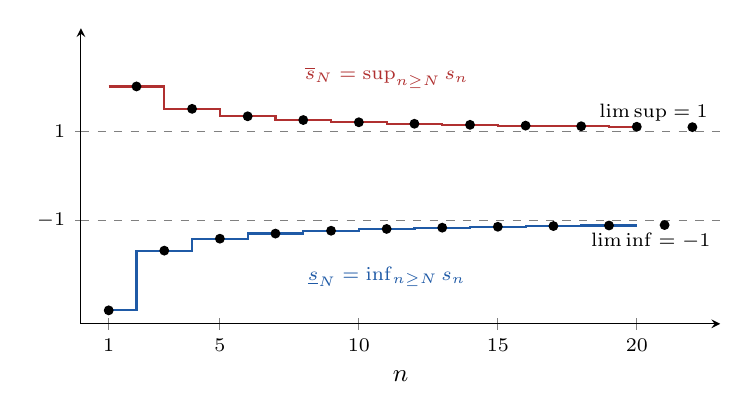
\begin{tikzpicture}
\begin{axis}[nfig, width=0.80\textwidth, height=0.44\textwidth,
  xmin=0, xmax=23, ymin=-3.3, ymax=3.3,
  xtick={1,5,10,15,20}, ytick={-1,1}, xlabel={$n$}]
  \addplot[black!50, dashed, thin] coordinates {(0,1) (23,1)};
  \addplot[black!50, dashed, thin] coordinates {(0,-1) (23,-1)};
  \addplot[figR, thick] coordinates {(1,2.0000) (2,2.0000) (2,2.0000) (3,2.0000) (3,1.5000) (4,1.5000) (4,1.5000) (5,1.5000) (5,1.3333) (6,1.3333) (6,1.3333) (7,1.3333) (7,1.2500) (8,1.2500) (8,1.2500) (9,1.2500) (9,1.2000) (10,1.2000) (10,1.2000) (11,1.2000) (11,1.1667) (12,1.1667) (12,1.1667) (13,1.1667) (13,1.1429) (14,1.1429) (14,1.1429) (15,1.1429) (15,1.1250) (16,1.1250) (16,1.1250) (17,1.1250) (17,1.1111) (18,1.1111) (18,1.1111) (19,1.1111) (19,1.1000) (20,1.1000)};
  \addplot[figB, thick] coordinates {(1,-3.0000) (2,-3.0000) (2,-1.6667) (3,-1.6667) (3,-1.6667) (4,-1.6667) (4,-1.4000) (5,-1.4000) (5,-1.4000) (6,-1.4000) (6,-1.2857) (7,-1.2857) (7,-1.2857) (8,-1.2857) (8,-1.2222) (9,-1.2222) (9,-1.2222) (10,-1.2222) (10,-1.1818) (11,-1.1818) (11,-1.1818) (12,-1.1818) (12,-1.1538) (13,-1.1538) (13,-1.1538) (14,-1.1538) (14,-1.1333) (15,-1.1333) (15,-1.1333) (16,-1.1333) (16,-1.1176) (17,-1.1176) (17,-1.1176) (18,-1.1176) (18,-1.1053) (19,-1.1053) (19,-1.1053) (20,-1.1053)};
  \addplot[only marks, mark=*, mark size=1.3pt, black] coordinates {(1,-3.0000) (2,2.0000) (3,-1.6667) (4,1.5000) (5,-1.4000) (6,1.3333) (7,-1.2857) (8,1.2500) (9,-1.2222) (10,1.2000) (11,-1.1818) (12,1.1667) (13,-1.1538) (14,1.1429) (15,-1.1333) (16,1.1250) (17,-1.1176) (18,1.1111) (19,-1.1053) (20,1.1000) (21,-1.0952) (22,1.0909)};
  \node[font=\scriptsize, figR] at (axis cs:11,2.2) {$\overline{s}_N = \sup_{n \geq N} s_n$};
  \node[font=\scriptsize, figB] at (axis cs:11,-2.25) {$\underline{s}_N = \inf_{n \geq N} s_n$};
  \node[font=\scriptsize] at (axis cs:20.6,1.42) {$\limsup = 1$};
  \node[font=\scriptsize] at (axis cs:20.5,-1.45) {$\liminf = -1$};
\end{axis}
\end{tikzpicture}\figcap{The envelopes at work for $s_n = (-1)^n\left(1 + \tfrac2n\right)$: the sequence (dots) has no limit, but the tail-suprema $\overline{s}_N$ (red, decreasing) and tail-infima $\underline{s}_N$ (blue, increasing) are monotone and bounded, so each converges --- to $\limsup = 1$ and $\liminf = -1$.}
\end{center}


\begin{propbox}[Lim Inf Is at Most Lim Sup]
$\displaystyle \liminf_{n\to+\infty} s_n \leq \limsup_{n\to+\infty} s_n$.
\end{propbox}

\begin{proof}
Why? Because $\underline{s}_N \leq \overline{s}_N$ for every $N$: the two are the $\inf$ and the $\sup$ of \emph{the same set} $\{s_n \mid n \geq N\}$, and for a nonempty set the infimum is $\leq$ the supremum (both compare with any single element). Passing to the limit in $N$ preserves $\leq$.
\end{proof}

If $\lim s_n$ exists, what is the relation? We expect $\liminf s_n \leq \lim s_n \leq \limsup s_n$. In fact, something stronger holds:

\begin{thmbox}[Convergence via Lim Sup and Lim Inf]
\begin{enumerate}[label=(\arabic*)]
    \item If $\lim_{n\to+\infty} s_n$ exists, then
    \[
    \liminf_{n\to+\infty} s_n = \limsup_{n\to+\infty} s_n = \lim_{n\to+\infty} s_n.
    \]
    \item Conversely, if $\liminf_{n\to+\infty} s_n = \limsup_{n\to+\infty} s_n$ (finite), then $\lim_{n\to+\infty} s_n$ exists --- $(s_n)$ is convergent, with this common value as limit.
\end{enumerate}
Part (2) gives another way to prove convergence of a sequence.
\end{thmbox}

\begin{proof}
(1) Let $s = \lim s_n$. For any $\varepsilon > 0$ there exists $N_0$ such that for all $n \geq N_0$,
\[
s - \varepsilon < s_n < s + \varepsilon.
\]
Taking the supremum and infimum over the tail $\{s_n \mid n \geq N\}$ for any $N \geq N_0$ (all its elements lie in $(s-\varepsilon,\, s+\varepsilon)$):
\[
s - \varepsilon \leq \underline{s}_N \leq \overline{s}_N \leq s + \varepsilon.
\]
Letting $N \to \infty$ (limits preserve $\leq$):
\[
s - \varepsilon \leq \liminf_{n\to\infty} s_n \leq \limsup_{n\to\infty} s_n \leq s + \varepsilon.
\]
Since $\varepsilon > 0$ is arbitrary, both $\liminf s_n$ and $\limsup s_n$ are squeezed to equal $s$.

(2) Let $s$ denote the common value. Given $\varepsilon > 0$: since $\underline{s}_N \to s$ and $\overline{s}_N \to s$, there exists $N'$ such that for all $N \geq N'$,
\[
s - \varepsilon < \underline{s}_N \qquad \text{and} \qquad \overline{s}_N < s + \varepsilon.
\]
Now for any $n \geq N'$, the term $s_n$ belongs to the tail starting at $n$, so $\underline{s}_n \leq s_n \leq \overline{s}_n$, giving
\[
s - \varepsilon < \underline{s}_n \leq s_n \leq \overline{s}_n < s + \varepsilon, \qquad \text{i.e.} \qquad |s_n - s| < \varepsilon.
\]
We are done. (Alternatively and more directly: $\underline{s}_n \leq s_n \leq \overline{s}_n$ with both outer sequences converging to $s$ --- apply the \emph{Squeeze Theorem}.)
\end{proof}

\subsection{Cauchy Sequences}

The concepts above give another way to prove convergence, but they still involve computing the limits $\limsup s_n$, $\liminf s_n$. \textbf{Question:} is there a way to decide convergence \emph{purely in terms of the sequence $(s_n)$ itself} --- no candidate limit, no auxiliary limits? \textbf{Answer: yes} --- the notion of Cauchy sequences.

\begin{defbox}[Cauchy Sequence]
A sequence $(s_n)$ is called \textbf{Cauchy} if for any $\varepsilon > 0$ there exists $N$ such that for any pair $m, n \geq N$,
\[
|s_n - s_m| < \varepsilon.
\]
Compare with the $(\varepsilon, N)$ definition of the limit: instead of comparing $s_n$ with a limit $s$, we compare the terms \emph{with each other}. The important point: the condition is purely in terms of $(s_n)$.
\end{defbox}

\begin{thmbox}[Convergent Implies Cauchy]
Every convergent sequence is a Cauchy sequence.
\end{thmbox}

\begin{proof}
Let $s = \lim s_n$. For any $\varepsilon > 0$ there exists $N$ such that $|s_n - s| < \tfrac\varepsilon2$ for all $n \geq N$. Then for any pair $m, n \geq N$,
\[
|s_n - s_m| = |s_n - s + s - s_m| \leq |s_n - s| + |s - s_m| < \frac\varepsilon2 + \frac\varepsilon2 = \varepsilon.
\]
So being Cauchy is a \emph{necessary} condition for convergence.
\end{proof}

\begin{thmbox}[Cauchy Implies Convergent]
If $(s_n)$ is a Cauchy sequence of real numbers, then $(s_n)$ is convergent. Combining with the previous theorem: \emph{$(s_n)$ is convergent if and only if it is Cauchy.}
\end{thmbox}

How to prove it? Not clear at first --- we must produce a limit out of nothing. Let us analyze: first check boundedness.

\begin{lembox}[Cauchy Implies Bounded]
If $(s_n)$ is Cauchy, then $(s_n)$ is bounded.
\end{lembox}

\begin{proof}
Let $\varepsilon = 1$: there exists $N$ such that $|s_n - s_m| < 1$ for all $m, n \geq N$. In particular, taking $m = N$: for all $n \geq N$,
\[
|s_n - s_N| < 1, \qquad \text{so} \qquad |s_n| < 1 + |s_N|.
\]
Do we have a bound yet? Not yet --- the initial terms again. Take
\[
M = \max\{|s_1|, \ldots, |s_{N-1}|,\ 1 + |s_N|\}.
\]
Then $|s_n| \leq M$ for all $n \geq 1$.
\end{proof}

\begin{proof}[Proof of the Theorem]
Since $(s_n)$ is bounded, $\liminf s_n$ and $\limsup s_n$ are finite. We use the criterion of the previous subsection: it suffices to show they are equal --- so we try to get information on $\underline{s}_N$, $\overline{s}_N$.

For any $\varepsilon > 0$ there exists $N$ such that for all $m, n \geq N$,
\[
-\varepsilon < s_n - s_m < \varepsilon.
\]
Taking $m = N$: for all $n \geq N$,
\[
s_N - \varepsilon < s_n < s_N + \varepsilon.
\]
Since this holds for \emph{every} $n \geq N$, we get --- crucially --- bounds on the whole tail:
\[
s_N - \varepsilon \leq \underline{s}_N \leq \overline{s}_N \leq s_N + \varepsilon.
\]
Since $(\underline{s}_N)$ is increasing and $(\overline{s}_N)$ is decreasing, for all $N' \geq N$ we retain $\underline{s}_{N} \leq \underline{s}_{N'} \leq \overline{s}_{N'} \leq \overline{s}_{N}$; letting $N' \to \infty$,
\[
s_N - \varepsilon \leq \liminf_{n\to\infty} s_n \leq \limsup_{n\to\infty} s_n \leq s_N + \varepsilon,
\]
hence
\[
0 \leq \limsup_{n\to\infty} s_n - \liminf_{n\to\infty} s_n \leq 2\varepsilon.
\]
Since $\varepsilon$ is arbitrary, squeezing between $0$ and $2\varepsilon$ forces
\[
\limsup_{n\to\infty} s_n = \liminf_{n\to\infty} s_n,
\]
and by the theorem of the previous subsection, $(s_n)$ is convergent.
\end{proof}

\begin{exbox}[A contraction-type estimate]
Assume $(s_n)$ satisfies $|s_{n+1} - s_n| < 2^{-n}$ for all $n \geq 1$. Prove $(s_n)$ is a Cauchy sequence, and hence convergent.

We need to see how big $|s_m - s_n|$ is for $m > n$. Telescope through the intermediate terms and apply the triangle inequality:
\[
|s_m - s_n| \leq |s_m - s_{m-1}| + |s_{m-1} - s_{m-2}| + \cdots + |s_{n+1} - s_n|
\leq 2^{-(m-1)} + \cdots + 2^{-n}.
\]
Summing the geometric progression,
\[
2^{-n} + \cdots + 2^{-(m-1)} = \frac{2^{-n} - 2^{-m}}{1 - \tfrac12} < \frac{2^{-n}}{1 - \tfrac12} = 2^{-n+1}.
\]
Note the right-hand side is \emph{independent of $m$}. Now, for any $\varepsilon > 0$, choose $N$ such that $2^{-N+1} < \varepsilon$ (possible since $2^{-N+1} \to 0$). Then for all $m \geq n \geq N$,
\[
|s_m - s_n| < 2^{-n+1} \leq 2^{-N+1} < \varepsilon,
\]
and we are done: $(s_n)$ is Cauchy, hence convergent. \hfill $\blacksquare$
\end{exbox}

\begin{rembox}[The geometric rate is doing the work (HW)]
It is \emph{not} enough that consecutive differences tend to $0$: the weaker hypothesis $|s_{n+1} - s_n| < \tfrac1n$ does not imply Cauchy. Counterexample:
\[
s_n = 1 + \frac12 + \frac13 + \cdots + \frac1n, \qquad |s_{n+1} - s_n| = \frac{1}{n+1} < \frac1n,
\]
yet $(s_n)$ is unbounded: grouping the terms in dyadic blocks,
\[
s_{2^k} = 1 + \frac12 + \underbrace{\left(\frac13 + \frac14\right)}_{>\, 2\cdot\frac14} + \underbrace{\left(\frac15 + \cdots + \frac18\right)}_{>\, 4\cdot\frac18} + \cdots \ >\ 1 + \frac k2,
\]
and since $(s_n)$ is increasing, it exceeds any $M$ from some point on. Unbounded sequences are not Cauchy. (These are the partial sums of the \emph{harmonic series}; the same dyadic estimate returns in \S 14.) The moral: in the example above, the increments were \emph{summable} --- the geometric tail $2^{-n+1}$ stayed uniformly small --- whereas mere decay of single increments controls nothing about the accumulated drift.
\end{rembox}

\begin{rembox}[Cauchy sequences and the construction of the reals]
Cauchy sequences can be used to construct $\mathbb{R}$ from $\mathbb{Q}$: real numbers can be identified with equivalence classes of Cauchy sequences of rational numbers (two sequences being equivalent when their difference tends to $0$). This is the second standard construction of $\mathbb{R}$, alongside the Dedekind cuts of \S 6. Note the logical order in this course, however: we \emph{assumed} $\mathbb{R}$ with completeness, and the theorem above (Cauchy $\Rightarrow$ convergent) is a \emph{consequence} --- indeed an equivalent form --- of the completeness axiom.
\end{rembox}

% ============================================================================
% SECTION 11: SUBSEQUENCES
% ============================================================================

\section{Subsequences}

We now want to understand the structure of sequences better. Recall: monotone $+$ bounded $\implies$ convergent, and both conditions are needed. If we remove boundedness, we still know what happens: an unbounded increasing sequence tends to $+\infty$, an unbounded decreasing one to $-\infty$. But what can we say about a \emph{bounded} sequence that is not monotone?

Consider $s_n = (-1)^n$, bounded but not convergent. All \emph{even} terms $s_{2n} = 1$ form a convergent sequence; all \emph{odd} terms $s_{2n+1} = -1$ form another. These are examples of \emph{subsequences} --- picking out only some of the terms.

\begin{defbox}[Subsequence]
Given a sequence $(s_n)$, a \textbf{subsequence} is a sequence $(t_k)$ of the form
\[
t_k = s_{n_k}, \qquad \text{where} \quad n_1 < n_2 < n_3 < \cdots.
\]
Usually we denote it by $(s_{n_k})$. Note that $n_k \to +\infty$ as $k \to +\infty$; in fact $n_k \geq k$ for all $k$ (by induction: $n_1 \geq 1$, and $n_{k+1} > n_k \geq k$ forces $n_{k+1} \geq k+1$).
\end{defbox}

\begin{exbox}[Subsequences of simple sequences]
For $s_n = n$: the even terms $(2k)$, the squares $(k^2)$, the primes, \ldots\ are all subsequences. For $s_n = 1 + (-1)^n \tfrac1n$: the sequence is not monotone, but the even-indexed subsequence $1 + \tfrac{1}{2k}$ is decreasing and the odd-indexed one $1 - \tfrac{1}{2k+1}$ is increasing --- monotone subsequences extracted from a non-monotone sequence.
\end{exbox}

\begin{thmbox}[Subsequences of a Convergent Sequence]
If $(s_n)$ converges, then every subsequence $(s_{n_k})$ also converges, to the same limit.
\end{thmbox}

\begin{proof}
Let $s = \lim s_n$. We must show: for any $\varepsilon > 0$ there exists $K$ such that $|s_{n_k} - s| < \varepsilon$ for $k \geq K$. By definition, there exists $N$ such that $|s_n - s| < \varepsilon$ for $n \geq N$. Since $n_k$ is strictly increasing and diverges to $+\infty$, there exists $K$ such that $n_k \geq N$ for all $k \geq K$; hence $|s_{n_k} - s| < \varepsilon$ for such $k$. (More directly: since $n_k \geq k$, we can simply take $K = N$.)
\end{proof}

\begin{corbox}[A Divergence Criterion]
If $(s_n)$ has two convergent subsequences converging to \emph{different} limits, then $(s_n)$ does not converge.
\end{corbox}

\begin{proof}
By contradiction: if $s_n \to s$, then by the theorem \emph{every} convergent subsequence converges to $s$ --- the two different limits would both equal $s$.
\end{proof}

Two useful strengthenings, both needed silently in arguments that ``pass to a further subsequence'':

\begin{propbox}[Subsequences of Subsequences (HW)]
A subsequence of a subsequence of $(s_n)$ is itself a subsequence of $(s_n)$.
\end{propbox}

\begin{proof}
Let $(t_k) = (s_{n_k})$ be a subsequence of $(s_n)$, and $(u_j) = (t_{k_j})$ a subsequence of $(t_k)$. Then
\[
u_j = t_{k_j} = s_{n_{k_j}},
\]
and the index map $j \mapsto n_{k_j}$ is strictly increasing: $j_1 < j_2$ gives $k_{j_1} < k_{j_2}$ ($(k_j)$ strictly increasing), which gives $n_{k_{j_1}} < n_{k_{j_2}}$ ($(n_k)$ strictly increasing). So $(u_j)$ is a subsequence of $(s_n)$ with indices $n_{k_j}$. (In functional language: a subsequence is a composition $s \circ \sigma$ with $\sigma: \mathbb{N} \to \mathbb{N}$ strictly increasing, and the composition $\sigma \circ \rho$ of two strictly increasing maps is strictly increasing.)
\end{proof}

\begin{propbox}[Subsequences and Infinite Limits (HW)]
If $s_n \to +\infty$, then every subsequence $(s_{n_k})$ also satisfies $s_{n_k} \to +\infty$; similarly for $-\infty$.
\end{propbox}

\begin{proof}
Given $M$, there is $N$ with $s_n > M$ for $n > N$. Since $n_k \geq k$ (proved with the definition), for all $k > N$ we have $n_k \geq k > N$, hence $s_{n_k} > M$. The case $-\infty$ is symmetric.
\end{proof}

\begin{rembox}
The converse of the theorem fails: convergence of \emph{a} subsequence does not imply convergence of the sequence --- $s_n = (-1)^n$ again.
\end{rembox}

\subsection{The Bolzano--Weierstrass Theorem}

The goal of this section:

\begin{thmbox}[Bolzano--Weierstrass]
Every bounded sequence $(s_n)$ has a convergent subsequence.
\end{thmbox}

This is what the example $s_n = (-1)^n$ leads us to expect.

\begin{proof}
(This proof is different from the book's.) Since $(s_n)$ is bounded, the tail-sup sequence $(\overline{s}_N)$ is also bounded, so
\[
\overline{s} = \limsup_{n\to\infty} s_n = \lim_{N\to\infty} \overline{s}_N
\]
is finite. We extract a subsequence converging to $\overline{s}$.

Fix $k \geq 1$ and use $\varepsilon = \tfrac1k$. Since $\overline{s}_N \downarrow \overline{s}$ (decreasing, \S 10), for every sufficiently large $n'$,
\[
\overline{s} \leq \overline{s}_{n'} \leq \overline{s} + \frac1k,
\]
and by monotonicity this holds for \emph{all larger} $n'$ as well --- so we may take $n'$ as large as we wish. Since $\overline{s}_{n'} = \sup\{s_n \mid n \geq n'\}$, the characterization of the supremum gives some index $N' \geq n'$ with
\[
s_{N'} \geq \overline{s}_{n'} - \frac1k.
\]
Combining the two displays,
\[
\overline{s} - \frac1k \leq \overline{s}_{n'} - \frac1k \leq s_{N'} \leq \overline{s}_{n'} \leq \overline{s} + \frac1k.
\]
Now do induction on $k$. For $k = 1$, get $n_1 = N'$. For $k = 2$, repeat the construction with $n'$ chosen \emph{bigger than $n_1$} --- this is important, and possible by the freedom in choosing $n'$ noted above --- to get $n_2 = N' > n_1$. And so on. We obtain a subsequence $(s_{n_k})$ satisfying
\[
\overline{s} - \frac1k \leq s_{n_k} \leq \overline{s} + \frac1k,
\]
and therefore $s_{n_k} \to \overline{s}$ by the Squeeze Theorem.

We could equally start with $\underline{s} = \liminf s_n$ and get another subsequence converging to it.
\end{proof}

\subsection{Subsequence Limits}

\begin{defbox}[Subsequence Limit]
Given a sequence $(s_n)$, a \textbf{subsequence limit} is any extended real number (including $\pm\infty$) that is the limit of some subsequence $(s_{n_k})$. We write $S$ for the set of all subsequence limits of $(s_n)$.
\end{defbox}

\begin{exbox}[Two subsequence limits]
For $s_n = (-1)^n$: $\overline{s} = 1$ and $\underline{s} = -1$, and $S = \{1, -1\}$ --- there are no other subsequence limits, by the argument in the next example.
\end{exbox}

\begin{exbox}[A limit at infinity]
Let $s_n = e^{(-1)^n n}$. Find all subsequence limits. The even terms $e^{2k} \to +\infty$; the odd terms $e^{-(2k+1)} \to 0$. So $0, +\infty \in S$. \emph{Why no more?} Every subsequence must contain infinitely many terms from at least one of these two special subsequences. A \emph{convergent} (in $[-\infty,+\infty]$) subsequence must contain infinitely many from \emph{only one} of them --- otherwise it contains two sub-subsequences with the different limits $0$ and $+\infty$, contradicting the subsequence theorem --- invoked here through both HW lemmas above: a sub-subsequence \emph{is} a subsequence of the original, and the theorem extends to the limit $+\infty$. And a subsequence drawing infinitely many terms from only one of the two behaves like that one. Hence $S = \{0, +\infty\}$. \hfill $\blacksquare$
\end{exbox}

\begin{exbox}[All of an interval]
The set of rational numbers in $[0,1]$ is countable (\S 2); make a list $(s_n)$ of them. Then $S = [0,1]$.

Two things to prove. \emph{Every subsequence limit belongs to $[0,1]$:} all terms lie in $[0,1]$, and limits preserve the inequalities $0 \leq s_{n_k} \leq 1$. \emph{Every $x \in [0,1]$ is a subsequence limit}, by the density of $\mathbb{Q}$ in $\mathbb{R}$ (\S 4): for each $k$, the interval $(x - \tfrac1k,\, x + \tfrac1k) \cap [0,1]$ contains infinitely many rationals, hence contains terms $s_n$ with $n$ arbitrarily large; choose inductively $n_k > n_{k-1}$ with $|s_{n_k} - x| < \tfrac1k$. Then $s_{n_k} \to x$. \hfill $\blacksquare$
\end{exbox}

\begin{exbox}[Designing the set of subsequence limits]
Produce a sequence whose set of subsequence limits is $[0, \tfrac12] \cup \{1\}$. List all rational numbers in $[0, \tfrac12]$ as the odd terms $s_{2n+1}$, and define all even terms $s_{2n} = 1$. By the arguments above, the odd part contributes exactly $[0, \tfrac12]$ and the even part contributes $\{1\}$.
\end{exbox}

\begin{thmbox}[Structure of the Set of Subsequence Limits]
For any sequence $(s_n)$, with $S$ its set of subsequence limits (in $[-\infty, +\infty]$):
\begin{enumerate}[label=(\arabic*)]
    \item $S$ is nonempty;
    \item $\sup S = \limsup_{n\to\infty} s_n$ and $\inf S = \liminf_{n\to\infty} s_n$;
    \item if $(s_n)$ is bounded, then $\max S$ exists and equals $\sup S$, and $\min S$ exists and equals $\inf S$.
\end{enumerate}
In particular, if $\limsup s_n = \liminf s_n$, then $S$ consists of a single element --- all convergent subsequences have the same limit.
\end{thmbox}

\begin{proof}
(1) If $(s_n)$ is bounded, the Bolzano--Weierstrass proof puts $\limsup s_n$ (and $\liminf s_n$) in $S$ already. If $(s_n)$ is not bounded --- say not bounded above --- then every tail is unbounded above, so we may choose inductively $n_1 < n_2 < \cdots$ with $s_{n_k} > k$; this subsequence tends to $+\infty$, so $+\infty \in S$. (Similarly $-\infty \in S$ if unbounded below.)

(2) We show $\limsup s_n$ is an upper bound of $S$. Let $s_0 \in S$, with subsequence $s_{n_k} \to s_0$. For every $k$, the term $s_{n_k}$ belongs to the tail starting at $n_k$, so
\[
s_{n_k} \leq \overline{s}_{n_k}.
\]
Now $(\overline{s}_{n_k})_k$ is a subsequence of $(\overline{s}_N)_N$, which converges to $\limsup s_n$ --- so it converges to the same limit (subsequence theorem; this answers the ``why''). Passing to the limit in the inequality,
\[
s_0 = \lim_k s_{n_k} \leq \lim_k \overline{s}_{n_k} = \limsup_{n\to\infty} s_n.
\]
So $\limsup s_n$ is an upper bound of $S$. Why is it \emph{equal} to $\sup S$? Because it happens to \emph{belong} to $S$ --- that is the content of the Bolzano--Weierstrass construction (and of (1) in the unbounded case, where $\limsup s_n = +\infty$). An upper bound that lies in the set is its supremum --- and its maximum. Similarly $\inf S = \liminf s_n$, attained as $\min S$; this also proves (3).
\end{proof}

\begin{rembox}
Using terms from topology (next section): $S$ is always a \emph{closed} subset of $\mathbb{R}$. Hence $S$ can never be, e.g., an open interval $(0,1)$; but $[0,1]$ or $[0,\tfrac12] \cup \{1\}$ are fine, as the examples showed.
\end{rembox}

% ============================================================================
% SECTION 12 (SKIPPED)
% ============================================================================

\section{Lim Sup and Lim Inf Continued (Skipped)}

This section of the book, dealing with further properties of $\limsup s_n$ and $\liminf s_n$, was skipped in lecture --- there is nothing really new in it beyond \S 10--\S 11. The section heading is kept so that the numbering of these notes stays aligned with the book and the lectures.

% ============================================================================
% SECTION 13: TOPOLOGICAL CONCEPTS IN METRIC SPACES
% ============================================================================

\section{Some Topological Concepts in Metric Spaces}

\subsection{Metric Spaces}

When we defined convergence of sequences of real numbers, the crucial thing was the absolute value $|s_n - s|$: it measures \emph{how close} $s_n$ is to $s$. As noted in \S 3, the absolute value gives a distance $d(a,b) = |a - b|$, whose triangle property $d(a,b) \leq d(a,c) + d(c,b)$ reflects the triangle inequality $|a+b| \leq |a| + |b|$. So the crucial structure is the notion of \emph{distance}. Abstracting it gives the notion of a metric space.

\begin{defbox}[Metric Space]
A \textbf{metric space} is a set $X$ with a function $d: X \times X \to \mathbb{R}$ satisfying three conditions:
\begin{enumerate}[label=(\arabic*)]
    \item for any $x, y \in X$: $d(x,y) \geq 0$, with equality $d(x,y) = 0$ if and only if $x = y$;
    \item $d(x,y) = d(y,x)$;
    \item for any three points $x, y, z \in X$: \quad $d(x,y) \leq d(x,z) + d(z,y)$.
\end{enumerate}
The function $d$ is called the \textbf{distance function}, or the \textbf{metric}.
\end{defbox}

\begin{rembox}[Reading the axioms]
(1) is the \emph{separation of points}: two different points must have positive distance. (2) is the \emph{symmetry} of distance --- equal in both directions; this may fail in real life (airfares!) and there are meaningful non-symmetric ``distances'' in mathematics too. (3) is the famous \emph{triangle inequality} --- often the condition that is not easy to verify.
\end{rembox}

\begin{exbox}[The real line]
$X = \mathbb{R}$ with $d(a,b) = |a - b|$: all three conditions were verified in \S 3.
\end{exbox}

\begin{exbox}[The complex plane]
$X = \mathbb{C}$. We need a notion of absolute value: for $z = x + iy$ with $x, y \in \mathbb{R}$, the \emph{complex conjugate} is $\overline{z} = x - iy$, and the \textbf{absolute value} (modulus) is
\[
|z| = \sqrt{z \overline{z}} = \sqrt{x^2 + y^2}.
\]
Define $d(z_1, z_2) = |z_1 - z_2|$. Conditions (1), (2) are easy. Condition (3) amounts to $|z_1 + z_2| \leq |z_1| + |z_2|$ --- not as easy.
\end{exbox}

\begin{rembox}[Proof of the complex triangle inequality]
Note $\operatorname{Re} w \leq |w|$ for any $w \in \mathbb{C}$, and $|z \overline{w}| = |z||w|$ (from $|zw|^2 = zw \cdot \overline{zw} = |z|^2 |w|^2$). Then
\[
|z_1 + z_2|^2 = (z_1 + z_2)\overline{(z_1 + z_2)} = |z_1|^2 + 2 \operatorname{Re}(z_1 \overline{z_2}) + |z_2|^2
\leq |z_1|^2 + 2 |z_1| |z_2| + |z_2|^2 = (|z_1| + |z_2|)^2,
\]
and take square roots.
\end{rembox}

\begin{exbox}[Euclidean space]
$X = \mathbb{R}^n$, $n \geq 1$. For $x = (x_1, \ldots, x_n)$ and $y = (y_1, \ldots, y_n)$, define the \textbf{Euclidean distance}
\[
d(x,y) = \sqrt{(x_1 - y_1)^2 + \cdots + (x_n - y_n)^2}.
\]
Again (1), (2) are easy and (3) is not (its proof goes through the Cauchy--Schwarz inequality; we defer it). When we identify $\mathbb{C} = \mathbb{R}^2$, this agrees with the distance on $\mathbb{C}$ above.
\end{exbox}

\begin{exbox}[The max distance]
Can we define a \emph{different} distance on $\mathbb{R}^n$? Yes:
\[
d_\infty(x,y) = \max\{|x_1 - y_1|, \ldots, |x_n - y_n|\}.
\]
Here condition (3) \emph{is} easy to check --- it reduces to $\mathbb{R}$ coordinate-wise: for each $i$,
\[
|x_i - y_i| \leq |x_i - z_i| + |z_i - y_i| \leq d_\infty(x,z) + d_\infty(z,y),
\]
and taking the maximum over $i$ on the left gives the triangle inequality for $d_\infty$.

\begin{center}
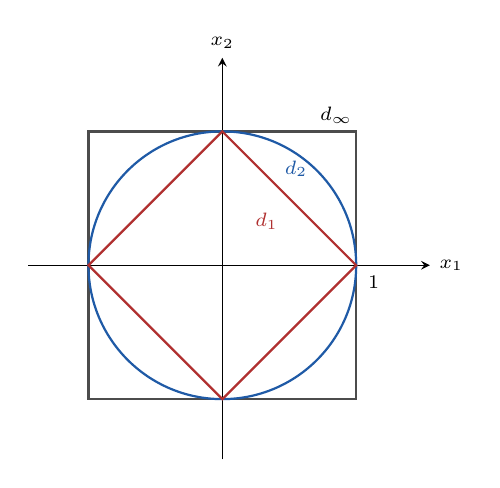
\begin{tikzpicture}[scale=1.7]
  \draw[-stealth, thin] (-1.45,0) -- (1.55,0) node[right, font=\scriptsize] {$x_1$};
  \draw[-stealth, thin] (0,-1.45) -- (0,1.55) node[above, font=\scriptsize] {$x_2$};
  \draw[black!70, thick] (-1,-1) rectangle (1,1);
  \draw[figB, thick] (0,0) circle (1);
  \draw[figR, thick] (1,0) -- (0,1) -- (-1,0) -- (0,-1) -- cycle;
  \node[font=\scriptsize, figR] at (0.33,0.33) {$d_1$};
  \node[font=\scriptsize, figB] at (0.55,0.72) {$d_2$};
  \node[font=\scriptsize] at (0.85,1.12) {$d_\infty$};
  \node[font=\scriptsize] at (1.13,-0.13) {$1$};
\end{tikzpicture}\figcap{The unit ball $\{ d(x, 0) \leq 1 \}$ in $\mathbb{R}^2$ for the three metrics: the taxicab diamond ($d_1$) inside the Euclidean disc ($d_2$) inside the max-distance square ($d_\infty$). Different geometry --- but each ball contains a scaled copy of the others, so all three metrics define the same convergent sequences.}
\end{center}

\end{exbox}

\begin{rembox}[Taxicabs in New York]
The lecture attached the name ``New York taxicab distance'' here, with the picture: in the Euclidean distance, the shortest path between two points is the straight segment --- but a taxicab in Manhattan can only move along a grid. Strictly speaking, the metric matching that picture is the \emph{sum} distance $d_1(x,y) = |x_1 - y_1| + \cdots + |x_n - y_n|$ (total grid driving), which is the one usually called the taxicab metric; the $d_\infty$ defined above is usually called the max (or Chebyshev) distance. Both are legitimate metrics on $\mathbb{R}^n$, both with coordinate-wise-easy triangle inequalities, and everything said below about $d_\infty$ holds for $d_1$ as well.
\end{rembox}

\subsection{Convergence and Completeness in Metric Spaces}

Once we have a metric space $(X, d)$, we can define convergence of sequences of points of $X$ --- the definitions are word-for-word those for $\mathbb{R}$, with $d$ in place of the absolute value.

\begin{defbox}[Convergence and Cauchy in a Metric Space]
Let $(s_n)$ be a sequence in a metric space $(X,d)$. We say $s_n \to s$ if for every $\varepsilon > 0$ there exists $N$ such that $d(s_n, s) < \varepsilon$ for all $n \geq N$. The sequence is \textbf{Cauchy} if for every $\varepsilon > 0$ there exists $N$ such that $d(s_n, s_m) < \varepsilon$ for all $m, n \geq N$.
\end{defbox}

\begin{rembox}[Positivity and uniqueness of limits]
The requirement $d(x,y) > 0$ for $x \neq y$ is used exactly to prove the \emph{uniqueness of limits}, by the same contradiction proof as in \S 7 (with $\varepsilon < \tfrac12 d(s,t)$). This is a good place to see what that condition is for; in general topology, the corresponding property of a space is called the \emph{Hausdorff property}.
\end{rembox}

\begin{propbox}[Equivalence of the Two Distances]
On $\mathbb{R}^n$,
\[
d_\infty(x,y) \leq d(x,y) \leq \sqrt{n}\, d_\infty(x,y).
\]
Consequently, $d$ and $d_\infty$ define the same class of convergent sequences (with the same limits) and the same class of Cauchy sequences.
\end{propbox}

\begin{proof}
For the first inequality: the largest $|x_i - y_i|$ satisfies $|x_i - y_i|^2 \leq \sum_j (x_j - y_j)^2$, so $d_\infty \leq d$. For the second: each of the $n$ summands is $\leq d_\infty(x,y)^2$, so $d(x,y)^2 \leq n\, d_\infty(x,y)^2$. Now check by the $(\varepsilon, N)$ definitions: if $d(s_n, s) \to 0$ then $d_\infty(s_n, s) \leq d(s_n,s) \to 0$; conversely if $d_\infty(s_n,s) \to 0$ then $d(s_n,s) \leq \sqrt{n}\, d_\infty(s_n,s) \to 0$ --- given $\varepsilon$, apply the $d_\infty$-definition with tolerance $\varepsilon/\sqrt{n}$. The same comparison works for the Cauchy condition.
\end{proof}

\begin{defbox}[Complete Metric Space]
A metric space $(X,d)$ is called \textbf{complete} if every Cauchy sequence in $X$ is convergent (to a point of $X$).
\end{defbox}

\begin{exbox}[Completeness of the real line]
$(\mathbb{R}, |\cdot|)$ is a complete metric space --- this is exactly what we proved in \S 10 (Cauchy $\Rightarrow$ convergent), and it is equivalent to the completeness axiom of $\mathbb{R}$.
\end{exbox}

\begin{thmbox}[Completeness of Euclidean Space]
$(\mathbb{R}^n, d)$ is a complete metric space (equivalently, $(\mathbb{R}^n, d_\infty)$ is).
\end{thmbox}

\begin{proof}
We reduce to $(\mathbb{R}, |\cdot|)$. The key point: a sequence $s_k = (x_{1,k}, \ldots, x_{n,k}) \in \mathbb{R}^n$ converges if and only if every \emph{coordinate sequence} $(x_{i,k})_{k}$ ($i = 1, \ldots, n$) converges in $\mathbb{R}$; and similarly for Cauchy. Both follow from
\[
|x_{i,k} - x_{i,m}| \leq d_\infty(s_k, s_m) \leq \max_i |x_{i,k} - x_{i,m}|
\]
(the right-hand inequality being an equality by definition).

So let $(s_k)$ be Cauchy in $\mathbb{R}^n$. Then each coordinate sequence $(x_{i,k})_k$ is Cauchy in $\mathbb{R}$ (left inequality, with $d_\infty \leq d$), hence converges, say $x_{i,k} \to x_i$, by the completeness of $\mathbb{R}$. Assemble $s = (x_1, \ldots, x_n)$. Then
\[
d(s_k, s) \leq \sqrt{n}\, d_\infty(s_k, s) = \sqrt{n} \max_i |x_{i,k} - x_i| \longrightarrow 0,
\]
since each of the finitely many coordinates tends to $0$. Hence $s_k \to s$.
\end{proof}

\begin{defbox}[Bounded Sequence in a Metric Space]
A sequence $(s_n)$ in $(X,d)$ is \textbf{bounded} if there exist a number $M > 0$ and a point $x_0 \in X$ such that $d(s_n, x_0) \leq M$ for all $n \geq 1$ --- a direct generalization of bounded sequences of real numbers.
\end{defbox}

\begin{thmbox}[Bolzano--Weierstrass in $\mathbb{R}^n$]
Every bounded sequence in $\mathbb{R}^n$ has a convergent subsequence.
\end{thmbox}

\begin{proof}[Proof sketch]
The proof is similar --- reduce to $\mathbb{R}$ coordinate by coordinate. If $(s_k)$ is bounded in $\mathbb{R}^n$, each coordinate sequence is bounded in $\mathbb{R}$. By Bolzano--Weierstrass in $\mathbb{R}$, extract a subsequence along which the first coordinates converge; from \emph{that} subsequence, extract a further subsequence along which the second coordinates converge (the first still converge, being a subsequence of a convergent sequence); continue through all $n$ coordinates. After $n$ extractions, all coordinates converge along the final subsequence, which therefore converges in $\mathbb{R}^n$ by the coordinate-wise criterion. So many things in calculus generalize to this topological setting.
\end{proof}

\subsection{Open and Closed Sets}

Now we can introduce the most important topological notions.

\begin{defbox}[Open and Closed Subsets]
Let $(X,d)$ be a metric space. A subset $U \subseteq X$ is called \textbf{open} if for every point $x \in U$, there exists a ball of some radius $\varepsilon > 0$ centered at $x$,
\[
B_d(x, \varepsilon) = \{ y \in X \mid d(y,x) < \varepsilon \},
\]
that is contained in $U$. A subset $C \subseteq X$ is called \textbf{closed} if the complement $X \setminus C$ is open.
\end{defbox}

The name ``open'' comes from open intervals in $\mathbb{R}$. These notions are the most important ones in topology: a \emph{topological space} can be described as a space together with its collection of open subsets --- equivalently, of closed subsets, since each collection determines the other by complementation.

\begin{exbox}[Open intervals are open]
Every open interval $(a,b) \subseteq \mathbb{R}$ is an open subset. For any $x \in (a,b)$: $x > a$ and $x < b$, so $x - a > 0$ and $b - x > 0$. Take $\varepsilon < \min\{x - a,\, b - x\}$; then $B(x,\varepsilon) = (x - \varepsilon, x + \varepsilon) \subseteq (a,b)$. \hfill $\blacksquare$

We \emph{cannot} do the same with the closed interval $[a,b]$ --- the argument fails at the endpoints: every ball around $a$ contains points $< a$, outside $[a,b]$. So closed intervals are not open subsets. (They are closed: the complement $(-\infty, a) \cup (b, +\infty)$ is open by the argument above.)
\end{exbox}

\begin{propbox}[Unions of Open Sets]
Any union of open subsets is open. Dually (by complementation), any intersection of closed subsets is closed.
\end{propbox}

\begin{proof}
If $x$ belongs to the union, it belongs to one of the open sets $U$, and the ball $B(x,\varepsilon) \subseteq U$ is contained in the union. The dual statement follows by De Morgan's laws.
\end{proof}

So, e.g., $(0,1) \cup (2,4)$ is open.

\begin{rembox}[Structure of open and closed subsets of the line]
\textbf{Fact:} every open subset of $\mathbb{R}$ is a union of open intervals --- possibly infinitely many, but always \emph{countably} many (one can take them disjoint). So open subsets of $\mathbb{R}$ have a simple description. Closed sets, by contrast, can be very complicated. Two illustrations:
\begin{itemize}
    \item Given any sequence $(s_n)$ in $\mathbb{R}$, its set $S$ of subsequence limits is a closed set (as promised in \S 11).
    \item \textbf{The Cantor set.} Start with $[0,1]$; remove the open middle third $(\tfrac13, \tfrac23)$, leaving the two closed intervals $[0,\tfrac13]$ and $[\tfrac23, 1]$; do the same to each of them, and continue by induction. What is left in the limit --- the intersection of all the stages --- is a closed subset of $[0,1]$ (an intersection of closed sets), very complicated but useful. It is \emph{not} a union of closed intervals: in fact it contains no interval at all.
\end{itemize}
\end{rembox}

\begin{propbox}[Sequential Characterization of Closedness]
$C \subseteq X$ is closed if and only if for every convergent sequence $s_n \to s$ in $X$ with all $s_n \in C$, the limit $s$ lies in $C$ too. So a closed set \emph{contains all limits of sequences of its points} --- that is why it is called closed.
\end{propbox}

\begin{proof}
($\Rightarrow$) Let $C$ be closed, $s_n \in C$, $s_n \to s$; suppose $s \notin C$. Then $s \in X \setminus C$, which is open, so some ball $B(s, \varepsilon) \subseteq X \setminus C$. But $d(s_n, s) < \varepsilon$ for large $n$, so $s_n \in B(s,\varepsilon) \subseteq X \setminus C$ --- contradicting $s_n \in C$. Hence $s \in C$.

($\Leftarrow$) Suppose $C$ is not closed, i.e.\ $X \setminus C$ is not open: there is a point $x \in X \setminus C$ such that no ball around $x$ is contained in $X \setminus C$. In particular, for each $n$ the ball $B(x, \tfrac1n)$ meets $C$: choose $s_n \in C \cap B(x, \tfrac1n)$. Then $d(s_n, x) < \tfrac1n \to 0$, so $s_n \to x$, with all $s_n \in C$ but $x \notin C$ --- the sequential condition fails. Contrapositively, the sequential condition implies closedness.
\end{proof}

\subsection{Closure}

One more important notion: how to produce closed sets from arbitrary sets.

\begin{defbox}[Closure]
For any subset $Y$ of a metric space $(X,d)$, the \textbf{closure} of $Y$, denoted $\overline{Y}$, is the smallest closed subset containing $Y$.
\end{defbox}

Why does such a smallest closed superset exist? Consider \emph{all} closed subsets containing $Y$ (there is at least one, namely $X$), and take their intersection: it is closed (intersection of closed sets is closed --- the dual of ``union of open is open''), it contains $Y$, and it is contained in every closed superset of $Y$. So it is the smallest one.

\begin{exbox}[Closures on the line]
If $Y$ is already closed, $\overline{Y} = Y$. For $Y = (a,b) \subset \mathbb{R}$: $\overline{Y} = [a,b]$. For $Y = \mathbb{Q}$, $X = \mathbb{R}$: what is $\overline{\mathbb{Q}}$? Answer: $\overline{\mathbb{Q}} = \mathbb{R}$ --- every real number is a limit of a sequence of rationals, by the density of $\mathbb{Q}$ in $\mathbb{R}$ (\S 4; choose $s_n \in \mathbb{Q} \cap (x - \tfrac1n, x + \tfrac1n)$).
\end{exbox}

\begin{propbox}[Sequential Characterization of the Closure]
\[
\overline{Y} = Y \cup \{ \lim s_n \mid (s_n) \text{ a convergent sequence with all } s_n \in Y \}.
\]
This makes it clear why $\overline{Y}$ is called the closure: it is $Y$ together with all the limits one can form from within $Y$.
\end{propbox}

\begin{exbox}[Two closures computed (HW)]
\textbf{(1)} $S = \left\{ \tfrac1n \mid n \in \mathbb{N} \right\}$: \quad $\overline S = S \cup \{0\}$.

The set $S \cup \{0\}$ is closed, since its complement
\[
(-\infty, 0) \ \cup\ \bigcup_{n=1}^{\infty} \left( \frac{1}{n+1},\ \frac1n \right) \ \cup\ (1, \infty)
\]
is a union of open intervals, hence open. And $0$ must belong to any closed set containing $S$, being the limit of the sequence $\tfrac1n \in S$ (sequential characterization). So $S \cup \{0\}$ is the smallest closed superset.

\textbf{(2)} $C = \{ r \in \mathbb{Q} \mid r^2 < 2 \} = \mathbb{Q} \cap (-\sqrt2, \sqrt2)$: \quad $\overline C = [-\sqrt2, \sqrt2]$.

($\subseteq$) $[-\sqrt2, \sqrt2]$ is closed and contains $C$: any limit of a sequence in $C$ obeys the bounds $-\sqrt2 \leq \lim \leq \sqrt2$, since limits preserve weak inequalities (\S 9).

($\supseteq$) Let $x \in [-\sqrt2, \sqrt2]$. For each $n$, the set $\left(x - \tfrac1n,\ x + \tfrac1n\right) \cap (-\sqrt2, \sqrt2)$ is a nonempty open interval (nonempty even at the endpoints: for $x = \sqrt2$ it contains $(\sqrt2 - \tfrac1n, \sqrt2)$), so the density of $\mathbb{Q}$ (\S 4) provides $r_n \in \mathbb{Q}$ inside it. Then $r_n \in C$ and $|r_n - x| < \tfrac1n$, so $x = \lim r_n \in \overline C$. (One uniform choice of interval replaces a case analysis over interior points and the two endpoints.)

This is the same set that exhibited the \emph{incompleteness} of $\mathbb{Q}$ in \S 4: within $\mathbb{Q}$ it has no least upper bound. Taking the closure within $\mathbb{R}$ fills in exactly the two missing points $\pm\sqrt2$.
\end{exbox}

% ============================================================================
% SECTION 14: SERIES
% ============================================================================

\section{Series}

We know how to add up finitely many numbers:
\[
a_1 + a_2, \qquad a_1 + a_2 + a_3, \qquad a_1 + \cdots + a_n = \sum_{k=1}^n a_k
\]
--- the $\Sigma$-notation being convenient, e.g.\ $\sum_{k=4}^{9} a_k = a_4 + a_5 + a_6 + a_7 + a_8 + a_9$.

\textbf{Question:} can we add up \emph{infinitely} many numbers, $a_1 + \cdots + a_n + \cdots$? People started thinking about this a long time ago; at the beginning, they thought it was impossible --- Zeno's paradox of Achilles and the tortoise. A long time later, it became clear. That is what we do now. Three test examples to keep in mind:
\[
\text{(1)} \quad 1 + 1 + 1 + \cdots \qquad
\text{(2)} \quad 1 + \frac12 + \frac1{2^2} + \frac1{2^3} + \cdots \qquad
\text{(3)} \quad 1 + \frac12 + \frac13 + \frac14 + \cdots
\]
Does each sum to a finite number? Example (2) is what resolves Zeno's paradox; in example (3) we are adding terms that become smaller and smaller --- does that suffice?

\begin{defbox}[Series and Partial Sums]
An \textbf{infinite series} (or a \textbf{series}) is an infinite sum
\[
a_1 + a_2 + \cdots = \sum_{n=1}^{\infty} a_n, \qquad a_n \in \mathbb{R}
\]
(it can also start at any index $m$: $\sum_{n=m}^\infty a_n$; we concentrate on $m = 1$). Its \textbf{partial sums} are
\[
s_n = \sum_{k=1}^{n} a_k,
\]
which form a sequence $(s_n)$.
\end{defbox}

\begin{defbox}[Convergence of a Series]
If the sequence $(s_n)$ of partial sums converges to a limit $s$, we say the series $\sum_{n=1}^\infty a_n$ \textbf{converges} to $s$ and write $\sum_{n=1}^\infty a_n = s$. If $(s_n)$ diverges, we say the series \textbf{diverges}; in the special case $s_n \to +\infty$ we say the series diverges to $+\infty$ and write $\sum_{n=1}^\infty a_n = +\infty$.
\end{defbox}

\begin{rembox}[Why is this definition reasonable?]
Only \emph{finite} sums are defined by the field operations of $\mathbb{R}$. An infinite sum must therefore be \emph{defined} in terms of finite ones --- and the natural way is as the limit of the finite approximations $s_n$, using the machinery of Chapter 2. This is also why series appear as a section of the chapter on sequences: a series \emph{is} a sequence, namely its sequence of partial sums.
\end{rembox}

\begin{exbox}[The three test examples]
\textbf{(1)} $a_n = 1$: then $s_n = n \to +\infty$, so $\sum_{n=1}^\infty 1 = +\infty$.

\textbf{(2)} $a_n = \dfrac{1}{2^{n-1}}$: the partial sum is a geometric sum,
\[
s_n = 1 + \frac12 + \cdots + \frac{1}{2^{n-1}} = \frac{1 - 2^{-n}}{1 - \tfrac12} = 2\left(1 - 2^{-n}\right).
\]
Is $(s_n)$ convergent? Yes: $2^{-n} \to 0$, so $\lim s_n = 2$, and
\[
\sum_{n=1}^\infty \frac{1}{2^{n-1}} = 2.
\]
The series converges --- Achilles does catch the tortoise.

\textbf{(3)} $a_n = \dfrac1n$ (the \emph{harmonic series}): now
\[
s_n = 1 + \frac12 + \frac13 + \cdots + \frac1n,
\]
and we cannot find a closed formula --- the situation is more complicated. We will need some tricks or theorems to show that in fact $s_n \to +\infty$: the harmonic series \emph{diverges}, even though its terms tend to $0$.
\end{exbox}

\subsection{The Cauchy Criterion for Series}

For the harmonic series we cannot find a closed formula for $s_n$, so we need to study general properties of series. Since a series \emph{is} the sequence of its partial sums, every convergence criterion for sequences transfers.

\begin{defbox}[Cauchy Criterion]
A series $\sum a_n$ is said to satisfy the \textbf{Cauchy criterion} if its sequence $(s_n)$ of partial sums is a Cauchy sequence. Explicitly, since for $m \geq n$
\[
s_m - s_{n-1} = a_n + a_{n+1} + \cdots + a_m,
\]
the criterion reads: for any $\varepsilon > 0$ there exists $N$ such that for all $m \geq n \geq N$,
\[
|a_n + a_{n+1} + \cdots + a_m| < \varepsilon.
\]
\end{defbox}

\begin{thmbox}[Cauchy Criterion for Series]
A series $\sum a_n$ converges if and only if it satisfies the Cauchy criterion.
\end{thmbox}

\begin{proof}
This is exactly the Cauchy condition for the convergence of the sequence $(s_n)$ (\S 10): convergent $\iff$ Cauchy.
\end{proof}

\begin{corbox}[Terms of a Convergent Series Tend to Zero]
If $\sum a_n$ converges, then $a_n \to 0$.
\end{corbox}

\begin{proof}
Take $m = n$ in the Cauchy criterion: for $n \geq N$, $|a_n| < \varepsilon$.
\end{proof}

\begin{propbox}[Linearity of Series]
If $\sum a_n$ and $\sum b_n$ converge and $c \in \mathbb{R}$, then
\[
\sum_{n=1}^\infty (a_n + b_n) = \sum_{n=1}^\infty a_n + \sum_{n=1}^\infty b_n
\qquad \text{and} \qquad
\sum_{n=1}^\infty c\,a_n = c \sum_{n=1}^\infty a_n.
\]
\end{propbox}

\begin{proof}
The partial sums obey $\sum_{k=1}^n (a_k + b_k) = s_n + t_n$ and $\sum_{k=1}^n c\,a_k = c\,s_n$ exactly (finite sums); now apply the limit theorems of \S 9 to the sequences $(s_n)$, $(t_n)$.
\end{proof}

\begin{corbox}[Convergent Plus Divergent Is Divergent (HW)]
If $\sum a_n$ converges and $\sum b_n$ diverges, then $\sum (a_n + b_n)$ diverges.
\end{corbox}

\begin{proof}
If $\sum(a_n + b_n)$ converged, then by linearity $\sum b_n = \sum\bigl((a_n + b_n) - a_n\bigr)$ would converge --- contradiction.
\end{proof}

\begin{rembox}
No conclusion holds for divergent plus divergent: $\sum \tfrac1n$ and $\sum\bigl(-\tfrac1n\bigr)$ both diverge, yet their sum is $\sum 0 = 0$. Typical use of the corollary: $\sum \tfrac{n-1}{n^2} = \sum\bigl( \tfrac1n - \tfrac1{n^2} \bigr)$ diverges, being (divergent harmonic) plus (convergent p-series with the sign flipped).
\end{rembox}

\begin{rembox}[Warning]
The converse is \textbf{not} true: $a_n \to 0$ does not imply that $\sum a_n$ converges. The counterexample is the harmonic series $\sum \tfrac1n$, as we now show.
\end{rembox}

\begin{thmbox}[Divergence of the Harmonic Series]
$\displaystyle\sum_{n=1}^{\infty} \frac1n = +\infty$, even though $\tfrac1n \to 0$.
\end{thmbox}

\begin{proof}
We show $s_n \to +\infty$ directly. First note $(s_n)$ is \emph{increasing} --- we add a positive amount at every step: $s_{n+1} = s_n + \tfrac{1}{n+1}$. Therefore it suffices to show that some \emph{subsequence} $s_{n_k} \to +\infty$ (an increasing sequence dominates its earlier terms, so the whole sequence follows its subsequence upward; for general sequences this implication fails!).

Try $n_k = 2^k$, dividing the sum into dyadic segments. Experiments first:
\[
s_{2} = 1 + \frac12 > \frac12, \qquad
s_{4} = 1 + \frac12 + \left(\frac13 + \frac14\right) > \frac12 + \left(\frac14 + \frac14\right) = \frac12 \cdot 2,
\]
\[
s_{8} = s_4 + \left(\frac15 + \frac16 + \frac17 + \frac18\right) > \frac12\cdot 2 + \left(\frac18 \cdot 4\right) = \frac12 \cdot 3.
\]
In general, the segment from $\tfrac{1}{2^{k-1}+1}$ to $\tfrac{1}{2^k}$ has $2^k - 2^{k-1} = 2^{k-1}$ terms, each $\geq \tfrac{1}{2^k}$, so the segment sums to more than
\[
\frac{1}{2^k} \cdot 2^{k-1} = \frac12.
\]
By induction, using $s_{2^{k-1}} > \tfrac12 (k-1)$, we get
\[
s_{2^k} > \frac12\, k.
\]
Hence $s_{2^k} \to +\infty$, and therefore $s_n \to +\infty$. This proof is a bit tricky; we will have more systematic proofs later (the integral test, \S 15).
\end{proof}

\begin{center}
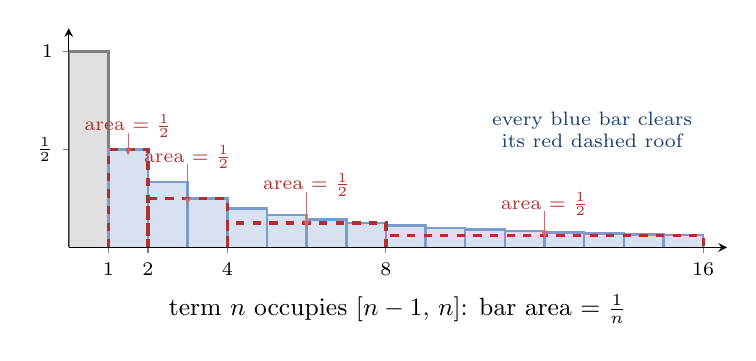
\begin{tikzpicture}
\begin{axis}[nfig, width=0.82\textwidth, height=0.36\textwidth,
  xmin=0, xmax=16.6, ymin=0, ymax=1.12,
  xtick={1,2,4,8,16}, ytick={0.5,1}, yticklabels={$\tfrac12$,$1$},
  xlabel={term $n$ occupies $[n-1,\,n]$: bar area $= \tfrac1n$}]
  \addplot[draw=black!50, fill=black!12] coordinates {(0,0) (0,1.0000) (1,1.0000) (1,0)};
  \addplot[draw=figB!60, fill=figB!18] coordinates {(1,0) (1,0.5000) (2,0.5000) (2,0)};
  \addplot[draw=figB!60, fill=figB!18] coordinates {(2,0) (2,0.3333) (3,0.3333) (3,0)};
  \addplot[draw=figB!60, fill=figB!18] coordinates {(3,0) (3,0.2500) (4,0.2500) (4,0)};
  \addplot[draw=figB!60, fill=figB!18] coordinates {(4,0) (4,0.2000) (5,0.2000) (5,0)};
  \addplot[draw=figB!60, fill=figB!18] coordinates {(5,0) (5,0.1667) (6,0.1667) (6,0)};
  \addplot[draw=figB!60, fill=figB!18] coordinates {(6,0) (6,0.1429) (7,0.1429) (7,0)};
  \addplot[draw=figB!60, fill=figB!18] coordinates {(7,0) (7,0.1250) (8,0.1250) (8,0)};
  \addplot[draw=figB!60, fill=figB!18] coordinates {(8,0) (8,0.1111) (9,0.1111) (9,0)};
  \addplot[draw=figB!60, fill=figB!18] coordinates {(9,0) (9,0.1000) (10,0.1000) (10,0)};
  \addplot[draw=figB!60, fill=figB!18] coordinates {(10,0) (10,0.0909) (11,0.0909) (11,0)};
  \addplot[draw=figB!60, fill=figB!18] coordinates {(11,0) (11,0.0833) (12,0.0833) (12,0)};
  \addplot[draw=figB!60, fill=figB!18] coordinates {(12,0) (12,0.0769) (13,0.0769) (13,0)};
  \addplot[draw=figB!60, fill=figB!18] coordinates {(13,0) (13,0.0714) (14,0.0714) (14,0)};
  \addplot[draw=figB!60, fill=figB!18] coordinates {(14,0) (14,0.0667) (15,0.0667) (15,0)};
  \addplot[draw=figB!60, fill=figB!18] coordinates {(15,0) (15,0.0625) (16,0.0625) (16,0)};
  \addplot[figR, dashed, very thick] coordinates {(1,0) (1,0.5) (2,0.5) (2,0)};
  \addplot[figR, dashed, very thick] coordinates {(2,0) (2,0.25) (4,0.25) (4,0)};
  \addplot[figR, dashed, very thick] coordinates {(4,0) (4,0.125) (8,0.125) (8,0)};
  \addplot[figR, dashed, very thick] coordinates {(8,0) (8,0.0625) (16,0.0625) (16,0)};
  \node[font=\scriptsize, figR] at (axis cs:1.5,0.62) {area $=\tfrac12$};
  \node[font=\scriptsize, figR] at (axis cs:3.0,0.46) {area $=\tfrac12$};
  \node[font=\scriptsize, figR] at (axis cs:6.0,0.32) {area $=\tfrac12$};
  \node[font=\scriptsize, figR] at (axis cs:12.0,0.22) {area $=\tfrac12$};
  \draw[figR!70, -stealth, very thin] (axis cs:1.5,0.585) -- (axis cs:1.5,0.47);
  \draw[figR!70, -stealth, very thin] (axis cs:3.0,0.425) -- (axis cs:3.0,0.22);
  \draw[figR!70, -stealth, very thin] (axis cs:6.0,0.285) -- (axis cs:6.0,0.105);
  \draw[figR!70, -stealth, very thin] (axis cs:12.0,0.185) -- (axis cs:12.0,0.05);
  \node[font=\scriptsize, figB!70!black, align=center] at (axis cs:13.2,0.60) {every blue bar clears\\ its red dashed roof};
\end{axis}
\end{tikzpicture}\figcap{The dyadic estimate as areas: term $n$ is a bar of area $\tfrac1n$; under each block of terms $(2^k, 2^{k+1}]$ sits a red dashed box of height $\tfrac{1}{2^{k+1}}$ (the block's smallest term) and width $2^k$ --- area exactly $\tfrac12$. Every bar clears its box's roof, so each block sums to at least $\tfrac12$, and the partial sums swallow one half-unit per block, forever.}
\end{center}


\subsection{Absolute Convergence}

\begin{defbox}[Absolute Convergence]
Given a series $\sum a_n$: if the series $\sum_{n=1}^\infty |a_n|$ converges, we say $\sum a_n$ \textbf{converges absolutely}.
\end{defbox}

\begin{propbox}[Absolute Convergence Implies Convergence]
If $\sum a_n$ converges absolutely, then it converges.
\end{propbox}

\begin{proof}
The only available proof is via the Cauchy criterion --- we cannot use the $(\varepsilon,N)$ definition directly, since we do not know the value of $\sum a_n$. Since $\sum |a_n|$ converges, it satisfies the Cauchy criterion: for any $\varepsilon > 0$ there is $N$ with
\[
|a_n| + \cdots + |a_m| < \varepsilon \qquad (m \geq n \geq N).
\]
\emph{Claim:} this implies $\sum a_n$ satisfies the Cauchy criterion too. Why? The triangle inequality:
\[
|a_n + \cdots + a_m| \leq |a_n| + \cdots + |a_m| < \varepsilon.
\]
Hence $\sum a_n$ converges.
\end{proof}

\begin{rembox}[Warning]
The converse is not true. The example to keep in mind: $a_n = (-1)^n \tfrac1n$. This series does \emph{not} converge absolutely --- $\sum |(-1)^n \tfrac1n| = \sum \tfrac1n$ diverges --- but we will show in \S 15 that $\sum (-1)^n \tfrac1n$ \emph{does} converge.
\end{rembox}

\subsection{The Comparison Test}

\begin{thmbox}[Comparison Test]
\begin{enumerate}[label=(\arabic*)]
    \item Assume $a_n \geq 0$ and $|b_n| \leq a_n$ for all $n$. If $\sum a_n$ converges, then $\sum b_n$ converges (absolutely).
    \item Assume $a_n \geq 0$ and $b_n \geq a_n$ for all $n$. If $\sum a_n$ diverges, then $\sum b_n$ diverges.
\end{enumerate}
\end{thmbox}

\begin{proof}
(1) By the Cauchy criterion for $\sum a_n$ and
\[
|b_n| + \cdots + |b_m| \leq a_n + \cdots + a_m < \varepsilon,
\]
the series $\sum |b_n|$ is Cauchy, hence converges; so $\sum b_n$ converges absolutely, and hence converges.

(2) Let $s_n = \sum_{k=1}^n a_k$ and $t_n = \sum_{k=1}^n b_k$. Then $t_n \geq s_n$ for all $n$. Since $a_n \geq 0$, the sequence $(s_n)$ is increasing, and divergence means $s_n \to +\infty$ (\S 10: an increasing sequence either converges or tends to $+\infty$). By the squeezing-to-infinity lemma (\S 9), $t_n \to +\infty$, so $\sum b_n$ diverges.
\end{proof}

\begin{propbox}[Bounded Multipliers Preserve Absolute Convergence (HW)]
If $\sum |a_n|$ converges and $(b_n)$ is a bounded sequence, then $\sum a_n b_n$ converges --- absolutely, in fact.
\end{propbox}

\begin{proof}
Let $|b_n| \leq M$ for all $n$. Then $|a_n b_n| \leq M |a_n|$, and $\sum M|a_n|$ converges; the comparison test finishes.
\end{proof}

\begin{rembox}
Three remarks. (1) Taking $b_n \equiv 1$ recovers ``absolute convergence implies convergence'' --- the proposition above becomes a special case. (2) This is the series analogue of the sequence fact ``null times bounded is null'' (\S 8). (3) It is also the germ of the \emph{Weierstrass M-test} of \S 25: there, $a_n$ becomes a convergent numerical majorant $M_n$ and $b_n$ a bounded family of function values, and the Cauchy-tail estimate $\left|\sum_{k=n+1}^m a_k b_k\right| \leq M \sum_{k=n+1}^m |a_k|$ --- an equally valid proof of this proposition --- reappears verbatim as the M-test's proof.
\end{rembox}

\begin{exbox}[Making the comparison go the right way]
Decide whether $\displaystyle\sum_{n=1}^{\infty} \frac{n}{n^2+2}$ converges or diverges.

\emph{Guess first:} the term is comparable to $\tfrac{n}{n^2} = \tfrac1n$, so it should diverge. But
\[
\frac{n}{n^2+2} < \frac{n}{n^2} = \frac1n,
\]
and a direct comparison with the divergent $\sum\tfrac1n$ goes the \emph{wrong way} --- being below a divergent series proves nothing. Instead bound from \emph{below}: for $n \geq 2$ (so that $n^2 \geq 2$),
\[
\frac{n}{n^2+2} \geq \frac{n}{n^2+n^2} = \frac{1}{2n}.
\]
Now $\sum \tfrac{1}{2n}$ diverges (scalar multiple of the harmonic series), so by comparison (2), our series diverges. Done! \hfill $\blacksquare$
\end{exbox}

To use the comparison test, we need a stock of basic series.

\begin{exbox}[The p-series]
For $p > 0$, the series
\[
\sum_{n=1}^\infty \frac{1}{n^p} \qquad \text{converges if and only if} \qquad p > 1.
\]
We proved divergence for $p = 1$; hence for $p < 1$ divergence follows by comparison, since $\tfrac{1}{n^p} \geq \tfrac1n$ when $p \leq 1$. The convergence for $p > 1$ will be proved by the integral test in \S 15. (The dyadic-block argument for the harmonic series was itself secretly a comparison --- we compared each block with a constant block from below.)
\end{exbox}

\begin{exbox}[The geometric series]
For $a \in \mathbb{R}$, the geometric series $\sum_{n=0}^\infty a^n$ converges if and only if $|a| < 1$, with
\[
\sum_{n=0}^\infty a^n = \frac{1}{1-a}, \qquad |a| < 1.
\]
Indeed $s_n = \tfrac{1 - a^{n+1}}{1 - a} \to \tfrac{1}{1-a}$ since $a^{n+1} \to 0$; while for $|a| \geq 1$ the terms do not tend to $0$, so the series diverges by the corollary above. This is the basic series against which the next two tests compare.
\end{exbox}

\subsection{The Ratio and Root Tests}

\begin{thmbox}[Ratio Test for Series]
Let $\sum a_n$ be a series with $a_n \neq 0$.
\begin{enumerate}[label=(\arabic*)]
    \item If $\limsup \left| \tfrac{a_{n+1}}{a_n} \right| < 1$, then $\sum a_n$ converges absolutely.
    \item If $\liminf \left| \tfrac{a_{n+1}}{a_n} \right| > 1$, then $\sum a_n$ diverges.
    \item If $\liminf \left| \tfrac{a_{n+1}}{a_n} \right| \leq 1 \leq \limsup \left| \tfrac{a_{n+1}}{a_n} \right|$: no information.
\end{enumerate}
Note the change from $\limsup$ (for convergence) to $\liminf$ (for divergence) --- using $\limsup$ and $\liminf$, no assumption that the ratio has a limit is needed.
\end{thmbox}

\begin{proof}
We compare with the geometric series.

(1) Pick $a$ with $\limsup |a_{n+1}/a_n| < a < 1$. Since the tail-sups decrease to the $\limsup$, there exists $N$ with $\sup_{n \geq N} |a_{n+1}/a_n| < a$, i.e.
\[
|a_{n+1}| < a\, |a_n| \qquad \text{for all } n \geq N.
\]
By induction, $|a_n| \leq a^{n-N} |a_N|$ for $n \geq N$. The series $\sum_n a^{n-N}|a_N|$ is a convergent geometric series ($0 < a < 1$), so $\sum |a_n|$ converges by comparison: $\sum a_n$ converges absolutely.

(2) Pick $b$ with $\liminf |a_{n+1}/a_n| > b > 1$. Since the tail-infs increase to the $\liminf$, there exists $N$ with $|a_{n+1}| > b |a_n| > |a_n|$ for all $n \geq N$. Then $|a_n| \geq |a_N| > 0$ for all $n \geq N$, so $a_n \not\to 0$, and the series diverges by the corollary (terms of a convergent series tend to $0$).

(3) Both $\sum \tfrac1n$ (divergent) and $\sum \tfrac1{n^2}$ (convergent) have ratio $\to 1$.
\end{proof}

\begin{thmbox}[Root Test]
Let $r = \limsup_{n\to\infty} |a_n|^{1/n}$.
\begin{enumerate}[label=(\arabic*)]
    \item If $r < 1$, then $\sum a_n$ converges absolutely.
    \item If $r > 1$, then $\sum a_n$ diverges.
    \item If $r = 1$: no information.
\end{enumerate}
\end{thmbox}

\begin{proof}
(1) Pick $a$ with $r < a < 1$. As above, there is $N$ with $|a_n|^{1/n} < a$, i.e.\ $|a_n| < a^n$, for all $n \geq N$; compare with the geometric series $\sum a^n$.

(2) If $r > 1$, then $|a_n|^{1/n} > 1$ --- i.e.\ $|a_n| > 1$ --- for infinitely many $n$ (a tail with all $|a_n|^{1/n} \leq 1$ would force $r \leq 1$). So $a_n \not\to 0$ and the series diverges.

(3) The same pair $\sum \tfrac1n$, $\sum \tfrac1{n^2}$: in both cases $|a_n|^{1/n} \to 1$ (using $n^{1/n} \to 1$ from \S 9).
\end{proof}

\begin{exbox}[Three quick applications]
Decide convergence or divergence, by any means:
\begin{enumerate}[label=(\arabic*)]
    \item $\displaystyle\sum \frac{3^n}{n^2}$: diverges --- the terms $\to +\infty$ (growth scale, \S 9); or ratio test: $\left|\tfrac{a_{n+1}}{a_n}\right| = 3 \left( \tfrac{n}{n+1} \right)^2 \to 3 > 1$.
    \item $\displaystyle\sum \frac{n^2}{3^n}$: converges absolutely --- ratio $\tfrac13 \left( \tfrac{n+1}{n} \right)^2 \to \tfrac13 < 1$.
    \item $\displaystyle\sum \frac{3^n}{n!}$: converges absolutely --- ratio $\tfrac{3}{n+1} \to 0 < 1$.
\end{enumerate}
\end{exbox}

% ============================================================================
% SECTION 15: ALTERNATING SERIES AND INTEGRAL TESTS
% ============================================================================

\section{Alternating Series and Integral Tests}

\subsection{Alternating Series}

\begin{thmbox}[Alternating Series Test]
If $a_1 \geq a_2 \geq a_3 \geq \cdots$ and $a_n \to 0$, then
\[
\sum_{n=1}^{\infty} (-1)^n a_n \quad \text{converges.}
\]
\end{thmbox}

\begin{rembox}
Note first that the hypotheses force $a_n \geq 0$ for all $n$: a decreasing sequence dominates its limit ($a_n \geq \lim_m a_m = 0$; if some $a_n < 0$, all later terms would be $\leq a_n < 0$, contradicting $a_n \to 0$). Note also that the condition $a_n \to 0$ is necessary --- why? --- because the terms $(-1)^n a_n$ of any convergent series must tend to $0$ (\S 14).
\end{rembox}

\begin{proof}
We check the Cauchy criterion: for any $\varepsilon > 0$ we need $N$ such that for $m \geq n \geq N$,
\[
\left| \sum_{k=n}^{m} (-1)^k a_k \right| < \varepsilon.
\]

\emph{Claim:} for all $m \geq n$,
\[
\left| \sum_{k=n}^{m} (-1)^k a_k \right| \leq a_n.
\]
This will be enough: given $\varepsilon$, choose $N$ with $a_n < \varepsilon$ for $n \geq N$ (possible since $a_n \to 0$).

\emph{Proof of the claim.} Factoring out the sign $(-1)^n$, the sum in question has absolute value
\[
\left| a_n - a_{n+1} + a_{n+2} - \cdots \pm a_m \right|,
\]
an alternating sum starting with $+a_n$. Group it in two ways. Grouping from the left in consecutive pairs,
\[
(a_n - a_{n+1}) + (a_{n+2} - a_{n+3}) + \cdots \geq 0,
\]
since each bracket is $\geq 0$ (decreasing) and a possible unpaired final term $+a_m$ is also $\geq 0$. Grouping instead with $a_n$ alone in front,
\[
a_n - (a_{n+1} - a_{n+2}) - (a_{n+3} - a_{n+4}) - \cdots \leq a_n,
\]
since each subtracted bracket is $\geq 0$ and a possible unpaired final term $-a_m$ is $\leq 0$. (The lecture checked the two parities on the examples $m = n+3$ and $m = n+2$; the displays above are the general case, which is the same.) So the alternating sum lies in $[0,\, a_n]$, proving the claim --- and the theorem. (The book has a different, longer proof.)
\end{proof}

\begin{exbox}[The alternating harmonic series]
$a_n = \tfrac1n$ satisfies the conditions (decreasing, $\to 0$), so
\[
\sum_{n=1}^{\infty} (-1)^n \frac1n \quad \text{converges}
\]
--- while, as promised in \S 14, it does not converge absolutely. Similarly $\sum (-1)^n \tfrac{1}{\sqrt n}$ converges (and not absolutely: $p = \tfrac12 \leq 1$).
\end{exbox}

\begin{exbox}[Convergence forces terms to die faster]
Assume $(a_n)$ is decreasing and $\sum a_n$ converges. Then
\[
\lim_{n\to\infty} n a_n = 0
\]
--- stronger than $\lim a_n = 0$.

\emph{Proof.} As above, decreasing $+$ summable forces $a_n \geq 0$. The series is Cauchy: for any $\varepsilon > 0$ there exists $N$ such that for $m \geq n \geq N$,
\[
a_{n+1} + \cdots + a_m < \varepsilon.
\]
Take $m = 2n$: since $(a_n)$ is decreasing, each of the $n$ terms $a_{n+1}, \ldots, a_{2n}$ is $\geq a_{2n}$, so
\[
\varepsilon > a_{n+1} + \cdots + a_{2n} \geq n\, a_{2n}, \qquad \text{hence} \qquad 2n\, a_{2n} < 2\varepsilon.
\]
So the even-indexed sequence $2n\, a_{2n} \to 0$. For the odd indices, $a_{2n+1} \leq a_{2n}$ gives
\[
(2n+1) a_{2n+1} \leq (2n+1) a_{2n} = 2n\, a_{2n} + a_{2n} \longrightarrow 0.
\]
Both subsequences of $(n a_n)$ covering all indices tend to $0$, hence $n a_n \to 0$. \hfill $\blacksquare$

Read contrapositively, this re-proves the divergence of the harmonic series in one line (HW): $\tfrac1n$ is decreasing, yet $n \cdot \tfrac1n = 1 \not\to 0$.
\end{exbox}

\begin{propbox}[Squares of a Nonnegative Convergent Series (HW)]
If $\sum a_n$ converges with $a_n \geq 0$ for all $n$, then $\sum a_n^2$ converges.
\end{propbox}

\begin{proof}
Since $\sum a_n$ converges, $a_n \to 0$ (\S 14), so there is $N$ with $0 \leq a_n < 1$ for $n \geq N$; for such $n$, $a_n^2 \leq a_n$. The tail $\sum_{n \geq N} a_n^2$ then converges by comparison with the convergent tail $\sum_{n \geq N} a_n$, and prepending the finitely many terms $a_1^2, \ldots, a_{N-1}^2$ does not affect convergence.
\end{proof}

\begin{rembox}[Neither converse holds (HW)]
Both implications between $\sum a_n$ and $\sum a_n^2$ fail in general:
\begin{enumerate}[label=(\arabic*)]
    \item $\sum a_n^2$ convergent $\not\Rightarrow$ $\sum a_n$ convergent: take $a_n = \tfrac1n$ ($\sum \tfrac{1}{n^2}$ converges, harmonic diverges).
    \item Without the sign condition, $\sum a_n$ convergent $\not\Rightarrow$ $\sum a_n^2$ convergent: take
    \[
    a_n = \frac{(-1)^n}{\sqrt n},
    \]
    convergent by the Alternating Series Theorem just proved ($\tfrac{1}{\sqrt n}$ decreasing to $0$) --- but $a_n^2 = \tfrac1n$, and the squares form the divergent harmonic series. \emph{Squaring destroys the sign cancellation that conditional convergence lives on.}
\end{enumerate}
\end{rembox}

\subsection{The Integral Test}

\begin{thmbox}[Integral Test]
Let $f: [1, +\infty) \to [0, +\infty)$ be a decreasing function. Then
\[
\sum_{n=1}^{\infty} f(n) \ \text{ converges} \qquad \Longleftrightarrow \qquad \int_1^{\infty} f(x)\, dx \ \text{ converges},
\]
and likewise the series diverges if and only if the integral diverges.
\end{thmbox}

\begin{proof}
The idea is to compare $\sum_{k=1}^n f(k)$ with $\int_1^n f(x)\,dx = \sum_{k=1}^{n-1} \int_k^{k+1} f(x)\,dx$. On each interval $[k, k+1]$, since $f$ is decreasing,
\[
f(k) \geq \int_k^{k+1} f(x)\, dx \geq f(k+1)
\]
(the integrand is trapped between its endpoint values on an interval of length $1$; e.g.\ $f(1) \geq \int_1^2 f \geq f(2)$). Summing over $k = 1, \ldots, n-1$ --- note the shift in index on the right:
\[
\sum_{k=1}^{n-1} f(k) \ \geq\ \int_1^n f(x)\, dx \ \geq\ \sum_{k=2}^{n} f(k) = s_n - f(1),
\]
where $s_n = \sum_{k=1}^n f(k)$. Since $f \geq 0$, both $(s_n)$ and $\left( \int_1^n f \right)$ are increasing, so each converges if and only if it is bounded (\S 10). The left inequality shows: $(s_n)$ bounded $\implies$ the integrals bounded. The right inequality shows: integrals bounded $\implies$ $s_n \leq f(1) + \int_1^n f$ bounded. Hence the two convergences are equivalent.
\end{proof}

\begin{center}
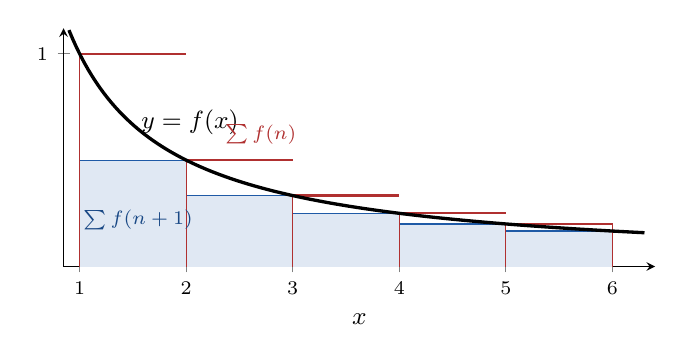
\begin{tikzpicture}
\begin{axis}[nfig, width=0.75\textwidth, height=0.38\textwidth,
  xmin=0.85, xmax=6.4, ymin=0, ymax=1.12,
  xtick={1,2,3,4,5,6}, ytick={1}, yticklabels={$1$}, xlabel={$x$}]
  \foreach \n in {1,...,5} {
    \edef\temp{\noexpand\addplot[draw=figB, fill=figB!14, thin]
      coordinates {(\n,0) (\n,{1/(\n+1)}) ({\n+1},{1/(\n+1)}) ({\n+1},0)};}
    \temp
  }
  \foreach \n in {1,...,5} {
    \edef\temp{\noexpand\addplot[figR, thick]
      coordinates {(\n,{1/\n}) ({\n+1},{1/\n})};}
    \temp
    \edef\tempb{\noexpand\addplot[figR, thin]
      coordinates {(\n,0) (\n,{1/\n})};}
    \tempb
  }
  \addplot[figR, thin] coordinates {(6,0) (6,0.2)};
  \addplot[black, very thick, domain=0.9:6.3, samples=150] {1/x}
    node[pos=0.13, right, font=\small] {$y=f(x)$};
  \node[figR, font=\scriptsize] at (axis cs:2.7,0.62) {$\sum f(n)$};
  \node[figB!80!black, font=\scriptsize] at (axis cs:1.55,0.22) {$\sum f(n+1)$};
\end{axis}
\end{tikzpicture}\figcap{The integral test for a decreasing $f$ (drawn: $f(x) = \tfrac1x$): the upper staircase (red, height $f(n)$ on $[n, n+1]$) and the lower staircase (blue, height $f(n+1)$) squeeze the curve, so partial sums and partial integrals are bounded together. The figure is the proof.}
\end{center}


\begin{exbox}[The p-series settled]
Let $f(x) = \tfrac{1}{x^p}$, $p > 0$ --- decreasing and nonnegative on $[1,\infty)$. From calculus,
\[
\int_1^n \frac{dx}{x^p} =
\begin{cases}
\ \dfrac{n^{1-p} - 1}{1-p} & p \neq 1, \\[2mm]
\ \log n & p = 1,
\end{cases}
\]
which stays bounded as $n \to \infty$ if and only if $1 - p < 0$. So $\int_1^\infty \tfrac{dx}{x^p}$ converges if and only if $p > 1$, and by the integral test,
\[
\sum_{n=1}^\infty \frac{1}{n^p} \ \text{ converges} \quad \Longleftrightarrow \quad p > 1,
\]
completing the claim of \S 14 (and re-proving the divergence of the harmonic series systematically). \hfill $\blacksquare$
\end{exbox}

\begin{rembox}
Like the logarithm in \S 9, the integral $\int_1^\infty f(x)\,dx$ is borrowed from the future: integration will be defined rigorously only in Part III. The comparison inequality $f(k) \geq \int_k^{k+1} f \geq f(k+1)$ and the computation of $\int \tfrac{dx}{x^p}$ are familiar from calculus and will be fully justified then; the logic of the test itself --- monotone partial sums, bounded iff convergent --- is already rigorous.
\end{rembox}

\begin{exbox}[The logarithmic ladder at the boundary (HW)]
How fine is the boundary $p = 1$? \textbf{First, comparison handles the easy cases.} Since $\log n \leq \sqrt n$ eventually (\S 9 scale), for large $n$
\[
\frac{1}{\sqrt n \log n} \geq \frac{1}{\sqrt n \cdot \sqrt n} = \frac1n, \qquad \frac{\log n}{n} \geq \frac1n,
\]
so $\sum \tfrac{1}{\sqrt n \log n}$ and $\sum \tfrac{\log n}{n}$ both diverge by comparison with the harmonic series --- no integral needed.

\textbf{The integral test is for the genuine boundary zone}, where the terms sit \emph{between} $\tfrac1n$ and every $\tfrac{1}{n^p}$ ($p > 1$), so no p-series comparison can decide. There the substitution $u = \log x$ exhibits a self-similar ladder:
\[
\int \frac{dx}{x \log x} = \log\log x \to \infty, \qquad
\int \frac{dx}{x \log x \, \log\log x} = \log\log\log x \to \infty, \qquad \ldots
\]
(each substitution turns a rung into the previous one), so
\[
\sum_{n\geq2} \frac{1}{n \log n}, \qquad \sum_{n\geq4} \frac{1}{n \log n \, \log\log n}, \qquad \ldots \quad \text{all diverge}
\]
--- divergence can be made arbitrarily slow, echoing the growth-scale remark of \S 9. By contrast, one extra \emph{power} rescues convergence immediately:
\[
\int_2^\infty \frac{\log x}{x^2}\,dx = \left[ -\frac{\log x}{x} - \frac1x \right]_2^\infty = \frac{\log 2 + 1}{2} < \infty
\]
(integration by parts; $\tfrac{\log x}{x} \to 0$ by the scale of \S 9), so $\sum \tfrac{\log n}{n^2}$ converges: a logarithm never overturns a power. \hfill $\blacksquare$
\end{exbox}

% ============================================================================
% SECTION 16 (NOT COVERED)
% ============================================================================

\section{Decimal Expansions of Real Numbers (Not Covered)}

This section of the book --- constructing decimal expansions of real numbers rigorously (thereby discharging the debt noted in \S 4) --- was not covered in lecture. The heading is kept to preserve the alignment of numbering with the book.

% ============================================================================
% CHAPTER 3: CONTINUITY
% ============================================================================

\chapter{Continuity}

% ============================================================================
% SECTION 17: CONTINUOUS FUNCTIONS
% ============================================================================

\section{Continuous Functions}

We now start a central chapter of this course: the notion of \emph{continuity}. You have all used continuous functions in calculus; now we will be rigorous.

\subsection{Two Definitions of Continuity}

Start with basics. Let $f: \Omega \to \mathbb{R}$ be a real-valued function defined on a subset $\Omega \subseteq \mathbb{R}$, called the \textbf{domain} of $f$, sometimes denoted $\operatorname{dom}(f)$. The domain can be any subset, but usually we take intervals --- closed $[a,b]$, open $(a,b)$, half-open --- and unions of them; this is related to the open and closed subsets of $\mathbb{R}$ discussed in \S 13. Determining the domain of a function is important, as we will see repeatedly.

\begin{defbox}[Continuity at a Point --- Sequential Definition]
$f: \Omega \to \mathbb{R}$ is said to be \textbf{continuous at $x_0 \in \Omega$} if for every sequence $(x_n)$ in $\Omega$ converging to $x_0$,
\[
f(x_n) \longrightarrow f(x_0).
\]
Intuitively: when $x \in \Omega$ is close to $x_0$, then $f(x)$ is close to $f(x_0)$.
\end{defbox}

\begin{exbox}[Linear and polynomial functions]
$f(x) = 2x$ on $\Omega = \mathbb{R}$ is continuous at every $x_0$: if $x_n \to x_0$, then $f(x_n) = 2x_n \to 2x_0 = f(x_0)$ by the scalar-multiple limit theorem. More generally, every polynomial
\[
f(x) = a_n x^n + a_{n-1}x^{n-1} + \cdots + a_0
\]
is continuous at every point --- by the limit theorems for sequences ($+$, $-$, $\times$) applied to $x_n \to x_0$.
\end{exbox}

For some functions the sequential definition is not so easy to check directly --- e.g.\ $f(x) = \sqrt{x}$ on $[0, +\infty)$: if $x_n \to x_0$ with $x_n \geq 0$, does $\sqrt{x_n} \to \sqrt{x_0}$ follow? (We did prove this in \S 8, but it took work.) We need another formulation, involving $\varepsilon$ as in the case of sequences.

\begin{thmbox}[The Epsilon-Delta Characterization]
$f$ is continuous at $x_0 \in \Omega$ if and only if: for every $\varepsilon > 0$, there exists $\delta > 0$ such that for every $x \in \Omega$ with $|x - x_0| < \delta$,
\[
|f(x) - f(x_0)| < \varepsilon.
\]
This is the $(\varepsilon, \delta)$ definition --- very basic and important; compare it with the $(\varepsilon, N)$ definition for sequences.
\end{thmbox}

\begin{proof}
($\Leftarrow$) Suppose the $(\varepsilon,\delta)$ condition holds, and let $x_n \to x_0$ with $x_n \in \Omega$. Given $\varepsilon > 0$, get the corresponding $\delta > 0$. By the $(\varepsilon, N)$ definition applied to the tolerance $\delta$, there exists $N$ such that $|x_n - x_0| < \delta$ for all $n \geq N$. Therefore $|f(x_n) - f(x_0)| < \varepsilon$ for all $n \geq N$, which shows $f(x_n) \to f(x_0)$.

($\Rightarrow$) Conversely, assume $f$ is continuous at $x_0$ in the sequential sense; we prove the $(\varepsilon,\delta)$ condition by contradiction. If it fails, there exists some $\varepsilon > 0$ such that for \emph{every} $\delta > 0$ there is a point $x_\delta \in \Omega$ with
\[
|x_\delta - x_0| < \delta \qquad \text{but} \qquad |f(x_\delta) - f(x_0)| \geq \varepsilon.
\]
For every $n \in \mathbb{N}$, apply this with $\delta = \tfrac1n$ to get $x_n \in \Omega$ with $|x_n - x_0| < \tfrac1n$ and $|f(x_n) - f(x_0)| \geq \varepsilon$. Then $x_n \to x_0$ but $f(x_n) \not\to f(x_0)$ --- contradicting the sequential continuity at $x_0$.
\end{proof}

\begin{center}
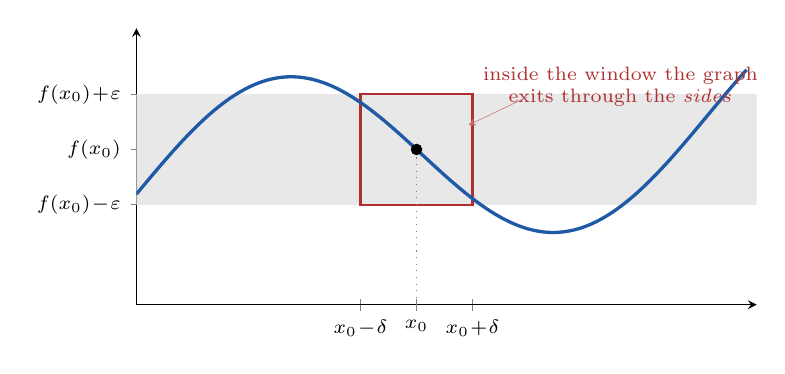
\begin{tikzpicture}
\begin{axis}[nfig, width=0.78\textwidth, height=0.42\textwidth,
  xmin=0, xmax=3.1, ymin=0.15, ymax=1.15,
  xtick={1.12,1.4,1.68}, xticklabels={$x_0\!-\!\delta$,$x_0$,$x_0\!+\!\delta$},
  ytick={0.5115,0.7115,0.9115},
  yticklabels={$f(x_0)\!-\!\varepsilon$,$f(x_0)$,$f(x_0)\!+\!\varepsilon$}, xlabel={}]
  \addplot[draw=none, fill=black!9] coordinates {(0,0.5115) (3.1,0.5115) (3.1,0.9115) (0,0.9115)};
  \draw[figR, thick] (axis cs:1.12,0.5115) rectangle (axis cs:1.68,0.9115);
  \addplot[figB, very thick, domain=0:3.05, samples=250] {0.55+0.35*sin(deg(2.2*x))+0.1*x};
  \addplot[only marks, mark=*, mark size=1.6pt, black] coordinates {(1.4,0.7115)};
  \draw[black!50, dotted] (axis cs:1.4,0.15) -- (axis cs:1.4,0.7115);
  \node[font=\scriptsize, figR] at (axis cs:2.42,0.98) {inside the window the graph};
  \node[font=\scriptsize, figR] at (axis cs:2.42,0.90) {exits through the \emph{sides}};
  \draw[figR!70, -stealth, very thin] (axis cs:1.95,0.90) -- (axis cs:1.66,0.80);
\end{axis}
\end{tikzpicture}\figcap{The $(\varepsilon, \delta)$ picture: the tolerance band $f(x_0) \pm \varepsilon$ (gray) is prescribed first; continuity provides a window $x_0 \pm \delta$ so narrow that over it the graph stays inside the band --- it leaves the red box through the sides, never the top or bottom. Outside the window the graph is free to escape the band (and here it does, on both sides): $\delta$ genuinely depends on $\varepsilon$ and on $x_0$. This is the third member of a family: the $(\varepsilon, N)$ band for sequences (\S 9), this local window, one window-width for \emph{all} points at once (uniform continuity, \S 19), and one band around a whole sequence of graphs (uniform convergence, \S 24).}
\end{center}


\begin{rembox}[Solving for delta]
In the $(\varepsilon,\delta)$ definition, $\delta$ depends on $\varepsilon$: we need to \emph{solve} $\delta$ in terms of $\varepsilon$. The idea, as with sequences: start with the target $|f(x) - f(x_0)| < \varepsilon$, \emph{simplify first} --- replace $|f(x)-f(x_0)|$ by a simpler upper bound if needed --- and then solve for $|x - x_0| < \delta = \delta(\varepsilon)$.
\end{rembox}

\begin{exbox}[A first epsilon-delta proof]
$f(x) = 3x$ is continuous at every $x_0 \in \mathbb{R}$. How to get $\delta$? Start with
\[
|f(x) - f(x_0)| = |3x - 3x_0| = 3|x - x_0| < \varepsilon \quad \iff \quad |x - x_0| < \tfrac13\varepsilon.
\]
So take $\delta = \tfrac13 \varepsilon$. \emph{Write-up:} for every $\varepsilon > 0$, let $\delta = \tfrac13\varepsilon$; when $|x - x_0| < \delta$, we get $|f(x) - f(x_0)| = 3|x-x_0| < 3 \cdot \tfrac13 \varepsilon = \varepsilon$. \hfill $\blacksquare$
\end{exbox}

\begin{exbox}[The square root]
$f(x) = \sqrt{x}: [0,+\infty) \to \mathbb{R}$ is continuous at every $x_0 \geq 0$. Two cases.

\textbf{Case $x_0 > 0$.} We want $|\sqrt x - \sqrt{x_0}| < \varepsilon$. By the conjugate,
\[
|\sqrt x - \sqrt{x_0}| = \left| \frac{x - x_0}{\sqrt x + \sqrt{x_0}} \right| \leq \frac{|x - x_0|}{\sqrt{x_0}},
\]
where the inequality replaces the denominator by the smaller $\sqrt{x_0}$ --- solving the original inequality exactly would be awkward; the simplified bound is what we solve. Setting $\tfrac{|x-x_0|}{\sqrt{x_0}} < \varepsilon$ gives $|x - x_0| < \varepsilon \sqrt{x_0}$, so take
\[
\delta = \varepsilon \sqrt{x_0}.
\]
Going back: when $|x - x_0| < \delta$ (and $x \geq 0$), the computation above gives $|\sqrt x - \sqrt{x_0}| < \varepsilon$.

\textbf{Case $x_0 = 0$.} The proof above fails --- why? We divided by $\sqrt{x_0} = 0$. Handle it directly: $f(0) = 0$, and we want $|\sqrt x| < \varepsilon$, which simplifies to $|x| < \varepsilon^2$. So take $\delta = \varepsilon^2$, and go back to verify. \hfill $\blacksquare$

It is important to note that $\delta$ depends on $\varepsilon$ \emph{and also on $x_0$} --- here $\delta = \varepsilon\sqrt{x_0}$ shrinks as $x_0$ approaches $0$. We will return to this point (uniform continuity).
\end{exbox}

\begin{exbox}[Damped oscillation]
Define $f: \mathbb{R} \to \mathbb{R}$ by $f(0) = 0$ and $f(x) = x \sin \tfrac1x$ for $x \neq 0$. Then $f$ is continuous at $x = 0$. Two ways:

(1) \emph{Sequences:} if $x_n \to 0$, then $|f(x_n) - f(0)| = |x_n \sin\tfrac{1}{x_n}| \leq |x_n| \to 0$ (null times bounded, \S 8; for terms with $x_n=0$ the value is $0$ anyway).

(2) \emph{$(\varepsilon,\delta)$:} for $x \neq 0$, $|f(x) - f(0)| = |x \sin\tfrac1x| \leq |x|$, so take $\delta = \varepsilon$.

In this case both are convenient; sometimes one is more convenient than the other. (About $\sin$: its rigorous definition comes later; here we use only the bound $|\sin t| \leq 1$.)
\end{exbox}

\begin{exbox}[Undamped oscillation]
Define $g: \mathbb{R} \to \mathbb{R}$ by $g(0) = 0$ and $g(x) = \sin\tfrac1x$ for $x \neq 0$. Then $g$ is \emph{not} continuous at $0$. How to prove it? Find a sequence $x_n \to 0$ with $g(x_n) \not\to 0 = g(0)$. As $x_n \to 0$, $\tfrac{1}{x_n} \to \infty$; choose the reciprocals to land where $\sin$ equals $1$:
\[
\frac{1}{x_n} = 2n\pi + \frac\pi2, \qquad \text{i.e.} \qquad x_n = \frac{1}{2n\pi + \tfrac\pi2} \longrightarrow 0,
\]
and $g(x_n) = \sin\left(2n\pi + \tfrac\pi2\right) = 1 \not\to 0$. \hfill $\blacksquare$
\end{exbox}

\begin{defbox}[Continuous Function]
A function $f: \Omega \to \mathbb{R}$ is called \textbf{continuous} if it is continuous at \emph{every} point $x_0 \in \Omega$.
\end{defbox}

\begin{rembox}[Continuity depends on the domain]
Granting that $\sin x$ is continuous everywhere (proved later), the function $g$ above is continuous at every $x \neq 0$ but not at $0$ --- so $g$ is not a continuous function. But if we define $G: \mathbb{R} \setminus \{0\} \to \mathbb{R}$, $G(x) = \sin\tfrac1x$, then $G$ \emph{is} continuous. The difference between $g$ and $G$? Only the domain: $\operatorname{dom}(G)$ omits the bad point. Likewise $f(x) = \tfrac1x$ with $\operatorname{dom}(f) = (0,+\infty)$ is continuous, while extending it to $[0,+\infty)$ by $g(0) = 0$ produces a non-continuous function. So the continuity of a function depends on its domain --- the domain is part of the definition of a function.
\end{rembox}

\subsection{Building Continuous Functions}

\begin{thmbox}[Absolute Value of a Continuous Function]
If $f$ is continuous at $x_0$, then $|f|$ is continuous at $x_0$.
\end{thmbox}

\begin{proof}
By the reverse triangle inequality,
\[
\bigl| |f(x)| - |f(x_0)| \bigr| \leq |f(x) - f(x_0)|,
\]
so any $\delta$ that works for $f$ (with tolerance $\varepsilon$) works for $|f|$.
\end{proof}

\begin{rembox}[The converse fails]
Define $f(x) = 1$ for $x \in \mathbb{Q}$ and $f(x) = -1$ for $x \in \mathbb{R}\setminus\mathbb{Q}$. Then $|f| \equiv 1$ is certainly continuous, but $f$ is continuous at \emph{no} point: at any $x_0$, by the density of $\mathbb{Q}$ and of $\mathbb{R}\setminus\mathbb{Q}$ (\S 4, and below), there are sequences $x_n \to x_0$ along which $f \equiv 1$ and sequences along which $f \equiv -1$; both $1$ and $-1$ cannot equal $f(x_0)$.
\end{rembox}

\begin{thmbox}[Arithmetic of Continuous Functions]
If $f, g$ are continuous at $x_0 \in \operatorname{dom}(f) \cap \operatorname{dom}(g)$, then:
\begin{enumerate}[label=(\arabic*)]
    \item $f \pm g$ is continuous at $x_0$;
    \item $fg$ is continuous at $x_0$;
    \item if $g(x_0) \neq 0$, then $f/g$ is continuous at $x_0$ (on the domain where $g \neq 0$).
\end{enumerate}
\end{thmbox}

\begin{proof}
It follows from the limit theorems for sequences (\S 9): if $x_n \to x_0$, then $f(x_n) \to f(x_0)$ and $g(x_n) \to g(x_0)$, so $f(x_n) \pm g(x_n) \to f(x_0) \pm g(x_0)$, $f(x_n)g(x_n) \to f(x_0)g(x_0)$, and (using $g(x_0) \neq 0$, quotient theorem) $f(x_n)/g(x_n) \to f(x_0)/g(x_0)$. One could also do it directly by the $(\varepsilon,\delta)$ definition.
\end{proof}

\begin{exbox}[Polynomials and rational functions]
(1) All polynomial functions are continuous --- we knew this already; it also follows from (1)--(2) starting with constants and $f(x)=x$. (2) Every rational function $\tfrac{P(x)}{Q(x)}$ is continuous at every point where the polynomial $Q$ does not vanish.
\end{exbox}

The most important and useful theorem in this section:

\begin{thmbox}[Composition of Continuous Functions]
Suppose $x_0 \in \operatorname{dom}(f)$ and $f(x_0) \in \operatorname{dom}(g)$ (with $f$ mapping into $\operatorname{dom}(g)$ near $x_0$, so the composition is defined). If $f$ is continuous at $x_0$ and $g$ is continuous at $f(x_0)$, then the composed function $g(f(x))$ is continuous at $x_0$.
\end{thmbox}

\begin{proof}
Suppose $x_n \to x_0$. Then $f(x_n) \to f(x_0)$ ($f$ continuous at $x_0$). Then $g(f(x_n)) \to g(f(x_0))$ ($g$ continuous at $f(x_0)$, applied to the sequence $f(x_n)$ in $\operatorname{dom}(g)$). Done! --- The sequential definition makes this proof effortless.
\end{proof}

\begin{exbox}[Compositions and domains]
When applying the composition theorem, \emph{check the domains}. (1) $f(x) = \tfrac1x$ is continuous at every $x \neq 0$, and $g(x) = \sin x$ is continuous (later); so $\sin\tfrac1x$ is continuous at every $x \neq 0$ --- as claimed above. (2) $f(x) = \sqrt{|x|}: \mathbb{R} \to \mathbb{R}$ is continuous everywhere: it is the composition of $|x|: \mathbb{R} \to [0,\infty)$ and $\sqrt{x}: [0,\infty) \to \mathbb{R}$, and the domain condition is satisfied since $|x|$ takes values exactly in $\operatorname{dom}(\sqrt{\ })$.
\end{exbox}

\begin{thmbox}[Max and Min of Continuous Functions]
If $f, g: [a,b] \to \mathbb{R}$ are continuous, then $\max\{f,g\}$ and $\min\{f,g\}$ are continuous.
\end{thmbox}

\begin{proof}
This is more complicated than the arithmetic operations --- until one finds the identity. \emph{Claim:}
\[
\max\{f,g\}(x) = \frac12\bigl(f(x) + g(x)\bigr) + \frac12\bigl|f(x) - g(x)\bigr|.
\]
Check both cases: if $f(x) > g(x)$, the right side is $\tfrac12(f+g) + \tfrac12(f-g) = f(x) = \max\{f,g\}(x)$; if $f(x) \leq g(x)$, it is $\tfrac12(f+g) + \tfrac12(g-f) = g(x) = \max\{f,g\}(x)$. Now combine the theorems: $f - g$ is continuous, hence $|f-g|$ is continuous, hence the whole right side is continuous (sums and scalar multiples). Similarly
\[
\min\{f,g\}(x) = \frac12\bigl(f(x)+g(x)\bigr) - \frac12\bigl|f(x)-g(x)\bigr|
\]
(or use $\min\{f,g\} = -\max\{-f,-g\}$).
\end{proof}

\subsection{Exotic Functions}

We have seen many continuous functions --- polynomials, rational functions, and later $\sin$, $\cos$, exponentials. How about some \emph{non}-continuous functions? Making use of the structures of the rational and real numbers, we can construct functions far stranger than the ordinary ones.

\begin{exbox}[Nowhere continuous]
The function $f = 1$ on $\mathbb{Q}$, $f = -1$ on $\mathbb{R}\setminus\mathbb{Q}$ above is continuous at no point --- yet $|f|$ is continuous. Can we make \emph{both} $g$ and $|g|$ discontinuous everywhere? Take
\[
g(x) = 1 \ (x \in \mathbb{Q}), \qquad g(x) = 0 \ (x \in \mathbb{R}\setminus\mathbb{Q}).
\]
Since $g \geq 0$, $|g| = g$, so it suffices that $g$ is nowhere continuous --- which follows by the same two-sequence argument at every point.
\end{exbox}

\begin{rembox}[Density of the irrationals]
These arguments use that $\mathbb{R} \setminus \mathbb{Q}$ is dense in $\mathbb{R}$: every interval $(a,b)$ contains irrational points. Why? The interval $(a,b)$ contains uncountably many points, but only countably many rationals (\S 2) --- so it must contain (uncountably many) irrationals. One can also argue directly: if $x_0 \in \mathbb{Q}$, the points $x_0 + \tfrac{\pi}{n}$ are irrational and converge to $x_0$.
\end{rembox}

\begin{exbox}[Continuous exactly at the irrationals]
Can we construct $f: \mathbb{R} \to \mathbb{R}$ that is continuous at every \emph{irrational} point but discontinuous at every \emph{rational} point? Not so easy --- but yes. Define
\[
f(x) = 0 \quad (x \in \mathbb{R}\setminus\mathbb{Q}); \qquad f\left(\frac pq\right) = \frac1q \quad \left( \frac pq \in \mathbb{Q} \text{ in lowest terms},\ q > 0 \right).
\]
(The lowest-terms representation with positive denominator is unique, so $f$ is well defined.)

\textbf{Discontinuity at rationals (the easy part).} Let $x_0 = \tfrac pq$, so $f(x_0) = \tfrac1q > 0$. Choose an irrational sequence $x_n \to x_0$ (density of irrationals above --- e.g.\ $x_n = x_0 + \tfrac\pi n$). Then $f(x_n) = 0 \not\to \tfrac1q = f(x_0)$. Not continuous.

\textbf{Continuity at irrationals (the harder part).} Let $x_0 \in \mathbb{R}\setminus\mathbb{Q}$, so $f(x_0) = 0$; take any $x_n \to x_0$; we must show $f(x_n) \to 0$. For irrational terms $f(x_n) = 0$ --- no problem. Assume for the moment all $x_n \in \mathbb{Q}$, written in lowest terms $x_n = \tfrac{p_n}{q_n}$.

\emph{Claim (1): $(q_n)$ is not bounded.} Suppose $q_n \leq M$ for all $n$. Since $\tfrac{p_n}{q_n} \to x_0$, the sequence is bounded: $\left|\tfrac{p_n}{q_n}\right| \leq C$, hence $|p_n| \leq C q_n \leq CM$. So only finitely many pairs $(p_n, q_n)$ occur --- the sequence $(x_n)$ takes only finitely many distinct values. A convergent sequence with finitely many values is eventually constant, so $x_0$ would equal that constant, a \emph{rational} number --- contradicting $x_0$ irrational.

\emph{Claim (2): in fact $q_n \to +\infty$.} If not, some subsequence $(q_{n_k})$ is bounded (negating $q_n \to +\infty$: there is $M$ such that for every $N$ some $n \geq N$ has $q_n \leq M$; extract inductively). But $\tfrac{p_{n_k}}{q_{n_k}} \to x_0$ still, so Claim (1) applied to the subsequence gives a contradiction.

Now finish: $f(x_n) = \tfrac{1}{q_n} \to 0 = f(x_0)$.

\emph{The general (mixed) sequence:} split $(x_n)$ into its irrational terms, along which $f \equiv 0$, and its rational terms, along which $f \to 0$ by the argument above (if there are infinitely many of them; finitely many don't matter). Given $\varepsilon > 0$, beyond some index every term of either kind has $f(x_n) < \varepsilon$; hence $f(x_n) \to 0$. So $f$ is continuous at every irrational point. \hfill $\blacksquare$
\end{exbox}

\begin{center}
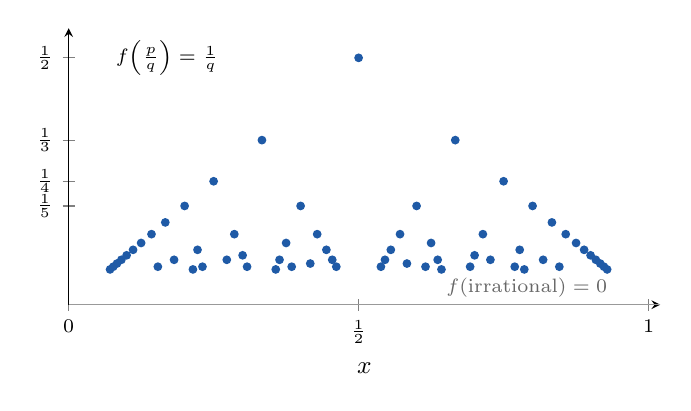
\begin{tikzpicture}
\begin{axis}[nfig, width=0.75\textwidth, height=0.42\textwidth,
  xmin=0, xmax=1.02, ymin=0, ymax=0.56,
  xtick={0,0.5,1}, xticklabels={$0$,$\tfrac12$,$1$},
  ytick={0.5,0.3333,0.25,0.2}, yticklabels={$\tfrac12$,$\tfrac13$,$\tfrac14$,$\tfrac15$}, xlabel={$x$}]
  \addplot[black!40, thin] coordinates {(0,0) (1.02,0)};
  \addplot[only marks, mark=*, mark size=1.1pt, figB] coordinates {(0.50000,0.50000) (0.33333,0.33333) (0.66667,0.33333) (0.25000,0.25000) (0.75000,0.25000) (0.20000,0.20000) (0.40000,0.20000) (0.60000,0.20000) (0.80000,0.20000) (0.16667,0.16667) (0.83333,0.16667) (0.14286,0.14286) (0.28571,0.14286) (0.42857,0.14286) (0.57143,0.14286) (0.71429,0.14286) (0.85714,0.14286) (0.12500,0.12500) (0.37500,0.12500) (0.62500,0.12500) (0.87500,0.12500) (0.11111,0.11111) (0.22222,0.11111) (0.44444,0.11111) (0.55556,0.11111) (0.77778,0.11111) (0.88889,0.11111) (0.10000,0.10000) (0.30000,0.10000) (0.70000,0.10000) (0.90000,0.10000) (0.09091,0.09091) (0.18182,0.09091) (0.27273,0.09091) (0.36364,0.09091) (0.45455,0.09091) (0.54545,0.09091) (0.63636,0.09091) (0.72727,0.09091) (0.81818,0.09091) (0.90909,0.09091) (0.08333,0.08333) (0.41667,0.08333) (0.58333,0.08333) (0.91667,0.08333) (0.07692,0.07692) (0.15385,0.07692) (0.23077,0.07692) (0.30769,0.07692) (0.38462,0.07692) (0.46154,0.07692) (0.53846,0.07692) (0.61538,0.07692) (0.69231,0.07692) (0.76923,0.07692) (0.84615,0.07692) (0.92308,0.07692) (0.07143,0.07143) (0.21429,0.07143) (0.35714,0.07143) (0.64286,0.07143) (0.78571,0.07143) (0.92857,0.07143)};
  \node[font=\scriptsize] at (axis cs:0.17,0.50) {$f\!\left(\tfrac pq\right) = \tfrac1q$};
  \node[font=\scriptsize, black!60] at (axis cs:0.79,0.035) {$f(\text{irrational}) = 0$};
\end{axis}
\end{tikzpicture}\figcap{The Thomae function on $(0,1)$, drawn for $q \leq 14$. The proof is visible: at any fixed height $\varepsilon$, only finitely many dots lie above it, so near an irrational point all nearby values of $f$ eventually drop below $\varepsilon$ --- continuity at every irrational, discontinuity at every rational.}
\end{center}


A counterweight to all these constructions --- continuity is \emph{rigid} on dense sets:

\begin{propbox}[Continuous Functions Are Determined on the Rationals (HW)]
Let $f, g: (a,b) \to \mathbb{R}$ be continuous with $f(r) = g(r)$ for every rational $r \in (a,b)$. Then $f(x) = g(x)$ for \emph{all} $x \in (a,b)$. In particular, a continuous function vanishing at every rational point of $(a,b)$ vanishes identically.
\end{propbox}

\begin{proof}
Let $h = f - g$, continuous on $(a,b)$ with $h(r) = 0$ for every rational $r \in (a,b)$; it suffices to show $h \equiv 0$. Fix $x_0 \in (a,b)$. For each $n$, the set
\[
\left( x_0 - \tfrac1n,\ x_0 + \tfrac1n \right) \cap (a,b)
\]
is a nonempty open interval ($x_0$ is an interior point of $(a,b)$), so the density of $\mathbb{Q}$ (\S 4) provides a rational $r_n$ inside it. Then $r_n \in (a,b)$, $r_n \to x_0$, and by the sequential definition of continuity,
\[
h(x_0) = \lim_{n\to\infty} h(r_n) = \lim_{n\to\infty} 0 = 0. \qedhere
\]
\end{proof}

\begin{rembox}
Nothing about $\mathbb{Q}$ was special except its \emph{density}: the same proof shows a continuous function is determined by its values on any dense subset (any $Y$ with $\overline{Y} \supseteq (a,b)$, in the closure language of \S 13). Read against the examples above, this is the price they pay: any function built to \emph{distinguish} $\mathbb{Q}$ from $\mathbb{R}\setminus\mathbb{Q}$ --- Dirichlet-type or Thomae-type --- is forced to be discontinuous somewhere, for a continuous function cannot tell a dense set apart from the whole line.
\end{rembox}

% ============================================================================
% SECTION 18: PROPERTIES OF CONTINUOUS FUNCTIONS
% ============================================================================

\section{Properties of Continuous Functions}

Now we come to one of the most exciting sections of this course. We have defined continuous functions and have examples. \emph{What can we do with them?} To use them, we need to know their properties --- to sharpen our tools. Throughout, the recurring theme: given $f$, the domain $\operatorname{dom}(f) = \Omega$ is part of the definition; now we want to understand the \textbf{image}
\[
\operatorname{Im}(f) = \{ f(x) \mid x \in \Omega \}.
\]

\subsection{The Extreme Value Theorem}

\begin{defbox}[Bounded Function]
A function $f: \Omega \to \mathbb{R}$ is called \textbf{bounded} if the set $\{f(x) \mid x \in \Omega\}$ is a bounded subset of $\mathbb{R}$: there exists $M > 0$ such that $|f(x)| \leq M$ for all $x \in \Omega$.
\end{defbox}

\begin{thmbox}[Extreme Value Theorem]
Let $\Omega = [a,b]$ be a finite closed interval and $f: [a,b] \to \mathbb{R}$ continuous. Then $f$ is bounded and \emph{achieves} its maximum and minimum values: there exist $x_0, y_0 \in [a,b]$ such that for every $x \in [a,b]$,
\[
f(y_0) \leq f(x) \leq f(x_0),
\]
i.e.\ $f(x_0) = \max \operatorname{Im}(f)$ and $f(y_0) = \min \operatorname{Im}(f)$.
\end{thmbox}

Boundedness is the basic beginning; the existence of max and min is very important in applications to optimization. In basic calculus one often \emph{assumes} they exist and works on finding them; here we address the more basic problem --- existence.

\begin{proof}
\textbf{Step 1: $f$ is bounded.} How to find a bound $M$? What is its value? No idea --- so we prove it by contradiction. If $f$ is not bounded, then for every $n \in \mathbb{N}$ there exists $x_n \in [a,b]$ with
\[
|f(x_n)| \geq n.
\]
Since $a \leq x_n \leq b$, the sequence $(x_n)$ is bounded. By the \textbf{Bolzano--Weierstrass Theorem} (\S 11), there is a convergent subsequence $x_{n_k} \to x_0$. \emph{Claim: $x_0 \in [a,b]$} --- because $a \leq x_{n_k} \leq b$ and limits preserve the inequalities. Since $f$ is continuous at $x_0$,
\[
f(x_{n_k}) \longrightarrow f(x_0);
\]
but $|f(x_{n_k})| \geq n_k \to \infty$, so $(f(x_{n_k}))$ is unbounded --- while every convergent sequence is bounded (\S 9). Contradiction. So $f$ is bounded.

\textbf{Step 2: the max is achieved} (the min is the same). By Step 1, $\operatorname{Im}(f)$ is a bounded (nonempty) subset of $\mathbb{R}$, so by the \textbf{completeness axiom}
\[
M = \sup \operatorname{Im}(f)
\]
exists. We need $x_0 \in [a,b]$ with $f(x_0) = M$. For any $n \in \mathbb{N}$, $M - \tfrac1n$ is not an upper bound of $\operatorname{Im}(f)$, so some point $x_n \in [a,b]$ has $f(x_n) > M - \tfrac1n$; combined with $f(x_n) \leq M$,
\[
M - \frac1n < f(x_n) \leq M.
\]
By Bolzano--Weierstrass again, extract $x_{n_k} \to x_0 \in [a,b]$ (as in Step 1). By continuity, $f(x_{n_k}) \to f(x_0)$; by the Squeeze Theorem along the subsequence of the displayed inequalities, $f(x_{n_k}) \to M$. By uniqueness of limits, $f(x_0) = M$. Done!
\end{proof}

\begin{rembox}[Toward optimization]
Application (borrowing differentiation from Part II): if $f$ is moreover differentiable on $(a,b)$ and the max point $x_0$ lies in the open interval $(a,b)$, then $x_0$ is a critical point, $f'(x_0) = 0$. So to find the maximum: find all critical points in $(a,b)$ and compare their values with the values at the endpoints $a, b$. The theorem above is what guarantees this recipe finds something.
\end{rembox}

\begin{rembox}[Both hypotheses are needed]
\textbf{(1) The interval must be closed (and finite):} $f(x) = \tfrac1x$ on $(0,1]$ is continuous, but $(0,1]$ is not closed, and $f$ is not bounded --- $f(\tfrac1n) = n \to \infty$. \textbf{(2) The function must be continuous:} $g: [0,1] \to \mathbb{R}$ with $g(0) = 0$, $g(x) = \tfrac1x$ for $x \in (0,1]$ is defined on a finite closed interval but is not continuous at $0$ --- and is not bounded.
\end{rembox}

Where \emph{exactly} does the proof need closedness? Reread Step 1 with $(a,b)$ in place of $[a,b]$ (HW): Bolzano--Weierstrass still extracts a convergent subsequence $x_{n_k} \to x_0$ --- but the load-bearing step is ``\emph{$x_0 \in [a,b]$, since limits preserve the endpoint inequalities}.'' For an open interval, $x_0$ may be an endpoint \emph{outside} the domain, and then $f(x_0)$ is not even defined --- the continuity argument has nowhere to land. And this failure is universal, not an accident of $\tfrac1x$:

\begin{propbox}[Non-Closed Sets Always Carry Unbounded Continuous Functions (HW)]
Let $S \subseteq \mathbb{R}$, and suppose some sequence $(x_n)$ in $S$ converges to a point $x_0 \notin S$. Then there exists a continuous unbounded function on $S$.
\end{propbox}

\begin{proof}
Take
\[
f(x) = \frac{1}{x - x_0}.
\]
Since $x_0 \notin S$, the denominator never vanishes on $S$, so $f$ is defined and continuous on $S$ (quotient of continuous functions). It is unbounded: given $M > 0$, convergence $x_n \to x_0$ provides $n$ with $0 < |x_n - x_0| < \tfrac1M$, and then
\[
|f(x_n)| = \frac{1}{|x_n - x_0|} > M. \qedhere
\]
\end{proof}

So the sets on which the boundedness conclusion of the EVT can possibly hold for \emph{all} continuous functions are exactly the sets containing all their sequential limits --- the \emph{closed} sets of \S 13.

\subsection{The Intermediate Value Theorem}

\begin{thmbox}[Intermediate Value Theorem]
Let $f: [a,b] \to \mathbb{R}$ be continuous. Then $f$ takes every value between $f(a)$ and $f(b)$: for any number $y$ between $f(a)$ and $f(b)$, there exists $x \in [a,b]$ with
\[
f(x) = y.
\]
\end{thmbox}

\begin{proof}
Simplify first. If $f(a) = f(b)$, the statement is clear --- the only value between them is $f(a)$ itself, achieved at both endpoints. So assume $f(a) \neq f(b)$; say $f(a) < f(b)$ (the case $f(a) > f(b)$ is the same, e.g.\ by applying the result to $-f$). If $y = f(a)$ or $y = f(b)$ we are done, so let $f(a) < y < f(b)$.

\emph{The idea:} start at $a$ and move toward $b$. Since the function is continuous --- we cannot jump --- we must meet the height $y$, like passing every intermediate altitude when climbing a mountain. To catch the moment we reach height $y$, define
\[
S = \{ x \in [a,b] \mid f(x) < y \}.
\]
(1) $S \neq \emptyset$: because $a \in S$ ($f(a) < y$). (2) $S$ is bounded: because $[a,b]$ is. By the completeness axiom, $x_0 = \sup S$ exists (and $x_0 \in [a,b]$: it is $\geq a$ since $a \in S$, and $\leq b$ since $b$ is an upper bound).

\emph{Claim: $f(x_0) = y$} --- reasonable, since $x_0$ is ``the last moment'' at height below $y$. We prove the equality by the two inequalities $\leq$ and $\geq$.

($\leq$) By the characterization of the supremum, there exists a sequence $x_n \in S$ with $x_n \to x_0$ (for each $n$, $x_0 - \tfrac1n$ is not an upper bound of $S$). Since $f$ is continuous and $f(x_n) < y$,
\[
f(x_0) = \lim_{n\to\infty} f(x_n) \leq y.
\]

($\geq$) From the inequality just proved, $f(x_0) \leq y < f(b)$, so $x_0 \neq b$, hence $x_0 < b$. Therefore, for all large $n$, $x_0 + \tfrac1n \leq b$, so $x_0 + \tfrac1n \in [a,b]$. Since $x_0 = \sup S$, the point $x_0 + \tfrac1n$ is \emph{not} in $S$, which means
\[
f\left(x_0 + \tfrac1n\right) \geq y.
\]
Since $x_0 + \tfrac1n \to x_0$ and $f$ is continuous at $x_0$, $f(x_0 + \tfrac1n) \to f(x_0)$, and limits preserve $\geq$:
\[
f(x_0) \geq y.
\]
So finally $f(x_0) = y$. Done!
\end{proof}

\begin{corbox}[Sign Change Gives a Root]
If $f: [a,b] \to \mathbb{R}$ is continuous and $f(a)$, $f(b)$ have opposite signs, then there exists $x_0 \in [a,b]$ with $f(x_0) = 0$.
\end{corbox}

\begin{proof}
$0$ lies between $f(a)$ and $f(b)$; apply the Intermediate Value Theorem.
\end{proof}

\begin{corbox}[The Image Is a Closed Interval]
For continuous $f: [a,b] \to \mathbb{R}$,
\[
\operatorname{Im}(f) = \bigl[\, \min \operatorname{Im}(f),\ \max \operatorname{Im}(f) \,\bigr]
\]
--- the image is again a finite closed interval. Continuous functions preserve finite closed intervals.
\end{corbox}

\begin{proof}
By the Extreme Value Theorem there are points $x_{\min}, x_{\max} \in [a,b]$ achieving $m = \min\operatorname{Im}(f)$ and $M = \max\operatorname{Im}(f)$, and $\operatorname{Im}(f) \subseteq [m, M]$. Conversely, assume $x_{\min} \leq x_{\max}$ (the other case is the same) and apply the Intermediate Value Theorem to the restriction $f: [x_{\min}, x_{\max}] \to \mathbb{R}$: $f$ takes every value between $f(x_{\min}) = m$ and $f(x_{\max}) = M$. So $[m,M] \subseteq \operatorname{Im}(f)$. Amazing! (This preservation property is the beginning of the topological notion of \emph{connectedness}: continuous images of path-connected spaces are path-connected.)
\end{proof}

\begin{rembox}[Descending the mountain]
The case $f(a) > f(b)$ can also be handled directly, without passing to $-f$: imagine coming \emph{down} from the peak. For $f(a) > y > f(b)$, define instead
\[
S = \{ x \in [a,b] \mid f(x) > y \}
\]
--- all the times spent \emph{above} height $y$; note $a \in S$. With $x_0 = \sup S$, the same proof as before gives $f(x_0) = y$.
\end{rembox}

\subsection{Applications of the Intermediate Value Theorem}

\begin{rembox}[The bisection algorithm]
The sign-change corollary can be upgraded to an \emph{algorithm} for approximating the root $x_0$:
\begin{enumerate}[label=(\arabic*)]
    \item Divide $[a,b]$ into two equal subintervals $[a,c]$, $[c,b]$, where $c = \tfrac12(a+b)$.
    \item If $f(c) = 0$, take $x_0 = c$: done. Otherwise, one of the pairs $f(a), f(c)$ or $f(c), f(b)$ has opposite signs --- why? because $f(a), f(b)$ do, and $f(c)$ agrees in sign with one of them. Keep the subinterval with the sign change; it contains a zero.
    \item Repeat. Each step halves the interval, so we narrow down $x_0$ quickly (error $\leq (b-a)/2^n$ after $n$ steps).
\end{enumerate}
\end{rembox}

\begin{thmbox}[Fixed Point Theorem on an Interval]
Let $f: [0,1] \to [0,1]$ be a continuous map. Then there exists $x_0 \in [0,1]$ with
\[
f(x_0) = x_0.
\]
Such a point --- mapped to itself --- is called a \textbf{fixed point}.
\end{thmbox}

\begin{proof}
A fixed point of $f$ is a zero of the function $g(x) = f(x) - x$, continuous on $[0,1]$. Check the endpoint values --- here the assumption that $f$ maps \emph{into} $[0,1]$ is what matters:
\[
g(0) = f(0) - 0 = f(0) \geq 0, \qquad g(1) = f(1) - 1 \leq 0.
\]
If either is zero, we are done. Otherwise $g(0) > 0$ and $g(1) < 0$ have opposite signs, and the sign-change corollary gives $x_0$ with $g(x_0) = 0$, i.e.\ $f(x_0) = x_0$.
\end{proof}

\begin{center}
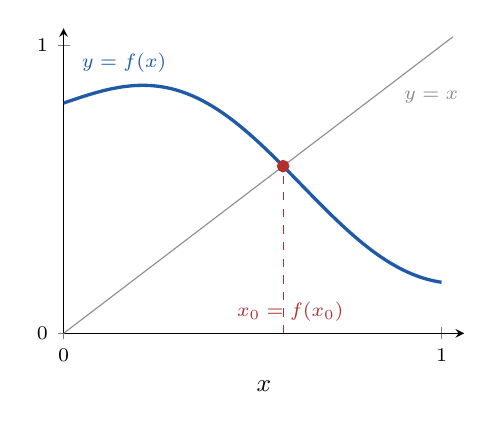
\begin{tikzpicture}
\begin{axis}[nfig, width=0.55\textwidth, height=0.45\textwidth,
  xmin=0, xmax=1.06, ymin=0, ymax=1.06,
  xtick={0,1}, ytick={0,1}, xlabel={$x$}]
  \addplot[black!45, thin, domain=0:1.03] {x} node[pos=0.85, below right, font=\scriptsize] {$y=x$};
  \addplot[figB, very thick, domain=0:1, samples=200] {0.8-0.45*x+0.18*sin(deg(5*x))};
  \addplot[only marks, mark=*, mark size=1.8pt, figR] coordinates {(0.5809,0.5809)};
  \draw[figR, dashed, thin] (axis cs:0.5809,0) -- (axis cs:0.5809,0.5809);
  \node[font=\scriptsize, figR] at (axis cs:0.60,0.075) {$x_0 = f(x_0)$};
  \node[font=\scriptsize, figB] at (axis cs:0.16,0.94) {$y=f(x)$};
\end{axis}
\end{tikzpicture}\figcap{The graph of $f: [0,1] \to [0,1]$ starts on or above the diagonal and ends on or below it --- so it must cross $y = x$. The same picture underlies the chord example below: two continuous curves that swap order must meet.}
\end{center}


\begin{exbox}[A chord of prescribed length]
Let $f: [0,2] \to \mathbb{R}$ be continuous with $f(0) = f(2)$. Prove there exist $x, y \in [0,2]$ with
\[
|y - x| = 1 \qquad \text{and} \qquad f(x) = f(y).
\]
Why should this be true? Draw the graph --- a curve returning to its starting height --- and slide a horizontal chord of length $1$ along it to convince yourself.

\emph{The real proof.} We need a new function to which the sign-change corollary applies. Define
\[
g(x) = f(x+1) - f(x), \qquad x \in [0,1]
\]
--- these are exactly the $x$ for which both $f(x)$ and $f(x+1)$ are defined. A zero $x_0$ of $g$ solves the problem, with $(x, y) = (x_0, x_0 + 1)$. Compute the endpoint values:
\[
g(0) = f(1) - f(0), \qquad
g(1) = f(2) - f(1) = f(0) - f(1) = -g(0),
\]
using $f(2) = f(0)$. So $g(0)$ and $g(1)$ are negatives of each other: either both are $0$ (done), or they have opposite signs, and the corollary gives the zero. \hfill $\blacksquare$
\end{exbox}

\begin{rembox}[Why fixed point theorems matter]
A fixed point theorem asserts the existence of a solution of an equation $f(x) = x$ --- and $f$ can be a continuous map from \emph{any} topological space to itself, not just $[0,1]$. For the unit square, the famous \textbf{Brouwer fixed point theorem} says every continuous $f: [0,1]^2 \to [0,1]^2$ has a fixed point; the same holds for the cube $[0,1]^3$ and in every dimension. (A cousin of this circle of ideas is the reason there is a spot on everyone's head where the hair cannot be combed flat.) Only in dimension one is there a simple proof, as above; higher dimensions require advanced tools of topology. In this general form, fixed point theorems are important far beyond mathematics --- in economics, game theory, and elsewhere.
\end{rembox}

Both applications above followed one pattern: build an auxiliary difference function and apply the sign-change corollary. The pattern itself deserves a statement:

\begin{propbox}[Crossing Lemma (HW)]
Let $f, g: [a,b] \to \mathbb{R}$ be continuous with
\[
f(a) \geq g(a) \qquad \text{and} \qquad f(b) \leq g(b).
\]
Then $f(x_0) = g(x_0)$ for at least one $x_0 \in [a,b]$: two continuous graphs that start and end on opposite sides must cross.
\end{propbox}

\begin{proof}
Let $h = f - g$, continuous on $[a,b]$, with $h(a) \geq 0$ and $h(b) \leq 0$. So $0$ lies between $h(b)$ and $h(a)$, and the Intermediate Value Theorem gives $x_0 \in [a,b]$ with $h(x_0) = 0$, i.e.\ $f(x_0) = g(x_0)$.
\end{proof}

\begin{rembox}
The Fixed Point Theorem is the special case $g(x) = x$ on $[0,1]$: the hypothesis $f([0,1]) \subseteq [0,1]$ says exactly $f(0) \geq g(0)$ and $f(1) \leq g(1)$. The chord example fits the pattern too, with $f(x+1)$ and $f(x)$ in the two roles.
\end{rembox}

\begin{propbox}[Odd-Degree Polynomials Have Real Roots (HW)]
Every polynomial $f(x) = a_0 + a_1 x + \cdots + a_{d} x^{d}$ of odd degree $d$ (with $a_d \neq 0$) has at least one real root.
\end{propbox}

\begin{proof}
We may assume $a_d > 0$ (otherwise pass to $-f$, which has the same roots). The idea: the leading term dominates far from the origin, so $f$ takes both signs; the IVT does the rest. To make ``dominates'' rigorous without limits of functions (\S 20 is still ahead), bound the lower-order part: let $C = |a_0| + \cdots + |a_{d-1}|$; then for $|x| \geq 1$,
\[
\bigl| a_0 + a_1 x + \cdots + a_{d-1} x^{d-1} \bigr| \leq C\,|x|^{d-1}.
\]
Take any $x_1 \geq \max\left\{ 1,\ \tfrac{2C}{a_d} \right\}$. Then
\[
f(x_1) \geq a_d x_1^{d} - C x_1^{d-1} = x_1^{d-1} \bigl( a_d x_1 - C \bigr) > 0,
\]
and at $x_2 = -x_1$, using that $d$ is \emph{odd} (so $x_2^{d} = -x_1^{d}$),
\[
f(x_2) \leq -a_d x_1^{d} + C x_1^{d-1} = x_1^{d-1}\bigl( C - a_d x_1 \bigr) < 0.
\]
Since $f$ is continuous on $[x_2, x_1]$ and $f(x_2) < 0 < f(x_1)$, the sign-change corollary gives $x_0 \in (x_2, x_1)$ with $f(x_0) = 0$.
\end{proof}

\begin{rembox}
Where does the argument use oddness? Only in the sign flip $(-x_1)^d = -x_1^d$. For even degree the conclusion genuinely fails: $x^2 + 1$ has no real root. And the choice of $x_1$ shows more than existence --- all real roots lie in $\left[ -\max\{1, \tfrac{2C}{a_d}\},\ \max\{1, \tfrac{2C}{a_d}\} \right]$, an explicit bound.
\end{rembox}

\subsection{Monotone Functions and Inverse Functions}

Recall $\operatorname{Im}(f) = f([a,b])$ is a bounded closed interval. Assuming $f(a) \leq f(b)$, is it equal to $[f(a), f(b)]$? \emph{Not in general} --- it can be much bigger.

\begin{exbox}[The image can exceed the endpoint values]
$f(x) = \sin x$ on $[0, 2\pi]$: here $\operatorname{Im}(f) = [-1, 1]$, but $f(0) = f(2\pi) = 0$, so $[f(a), f(b)] = \{0\}$, a single point.
\end{exbox}

In one special case, equality does hold.

\begin{defbox}[Strictly Monotone Functions]
$f: [a,b] \to \mathbb{R}$ is \textbf{strictly increasing} if $x_1 > x_2$ implies $f(x_1) > f(x_2)$ (e.g.\ $2x$, $x^3$), and \textbf{strictly decreasing} if $x_1 > x_2$ implies $f(x_1) < f(x_2)$. The two are related by the operations $f \mapsto -f$ and (for positive $f$) $f \mapsto \tfrac1f$: e.g.\ $e^{-x} = \tfrac{1}{e^x}$ and $-e^x$ are strictly decreasing.
\end{defbox}

\begin{thmbox}[Continuous Inverse Theorem]
If $f: [a,b] \to \mathbb{R}$ is a strictly increasing continuous function, then $\operatorname{Im}(f) = [f(a), f(b)]$, and the inverse function
\[
f^{-1}: [f(a), f(b)] \to [a,b]
\]
exists and is a strictly increasing continuous function. (Similarly, for strictly decreasing $f$: $\operatorname{Im}(f) = [f(b), f(a)]$ and $f^{-1}$ is strictly decreasing and continuous.)
\end{thmbox}

\begin{proof}
\textbf{The image.} By strict monotonicity, $f(a)$ is the minimum value and $f(b)$ the maximum; by the closed-interval corollary above, $\operatorname{Im}(f) = [f(a), f(b)]$.

\textbf{Existence of $f^{-1}$.} For every $y \in [f(a), f(b)]$ there exists $x \in [a,b]$ with $f(x) = y$ (Intermediate Value Theorem), and this $x$ is \emph{unique}: any other $x_1 \neq x$ has $f(x_1) \neq f(x)$ by strict monotonicity. So $f^{-1}(y) = x$ is well defined.

\textbf{Continuity of $f^{-1}$.} Fix $y_0 \in [f(a), f(b)]$ and any sequence $y_n \to y_0$ in $[f(a), f(b)]$; we must show $f^{-1}(y_n) \to f^{-1}(y_0)$. The sequence $x_n = f^{-1}(y_n) \in [a,b]$ is bounded. Suppose it does \emph{not} converge to $f^{-1}(y_0)$. Then there exist $\varepsilon > 0$ and a subsequence with $|x_{n_k} - f^{-1}(y_0)| \geq \varepsilon$ for all $k$; by Bolzano--Weierstrass, extract a further subsequence (still denoted $x_{n_k}$) converging to some $x_0 \in [a,b]$, and passing to the limit in the inequality, $|x_0 - f^{-1}(y_0)| \geq \varepsilon$, so
\[
x_0 \neq f^{-1}(y_0).
\]
Since $f$ is continuous, $f(x_{n_k}) \to f(x_0)$; but $f(x_{n_k}) = y_{n_k} \to y_0$. By the uniqueness of limits, $y_0 = f(x_0)$, i.e.\ $x_0 = f^{-1}(y_0)$ --- contradicting the display. So $x_n \to f^{-1}(y_0)$, and $f^{-1}$ is continuous at $y_0$.

\textbf{$f^{-1}$ is strictly increasing.} By contradiction: if not, there exist $y_1 < y_2$ with $f^{-1}(y_1) \geq f^{-1}(y_2)$. Applying the increasing $f$ preserves $\geq$:
\[
y_1 = f(f^{-1}(y_1)) \geq f(f^{-1}(y_2)) = y_2,
\]
a contradiction.
\end{proof}

\begin{rembox}[Beyond closed intervals]
The theorem extends to strictly monotone continuous functions on intervals of any type (open, half-open, infinite): apply it on closed subintervals exhausting the domain. The standard application: granting that $e^x: \mathbb{R} \to (0, +\infty)$ is strictly increasing and continuous (rigorous treatment of $e^x$ later), its inverse
\[
\log: (0, +\infty) \to \mathbb{R}
\]
exists and is continuous --- finally putting the logarithm, borrowed on credit in \S 9, on firmer footing (its continuity, at least; its defining properties still await the rigorous $e^x$).
\end{rembox}

% ============================================================================
% SECTION 19: UNIFORM CONTINUITY
% ============================================================================

\section{Uniform Continuity}

In the $(\varepsilon, \delta)$ definition of continuity, one important point: $\delta$ depends on $\varepsilon$ \emph{and on the point $x_0$}. This was very clear for $f(x) = \sqrt{x}$, where $\delta = \varepsilon\sqrt{x_0}$ shrank as $x_0 \to 0$ (\S 17). For some applications we want a choice of $\delta$ \emph{independent of $x_0$} --- depending only on $\varepsilon$: a uniform criterion for all points of the domain.

\begin{defbox}[Uniform Continuity]
$f: \Omega \to \mathbb{R}$ is called \textbf{uniformly continuous} if for every $\varepsilon > 0$ there exists $\delta > 0$ such that for \emph{every pair} $x, y \in \Omega$ with $|x - y| < \delta$,
\[
|f(x) - f(y)| < \varepsilon.
\]
The idea: whenever $x, y$ are close, $f(x), f(y)$ are close --- \emph{no matter where they are}. The condition is uniform, or fair, to every pair.
\end{defbox}

\begin{rembox}
Compare quantifiers with ordinary continuity: there, ``$\forall x_0\, \forall \varepsilon\, \exists \delta$'' --- here, ``$\forall \varepsilon\, \exists \delta\, \forall$ pairs''. Uniform continuity implies continuity at every point (freeze $y = x_0$); the converse fails, as the next example shows.
\end{rembox}

\begin{exbox}[The two faces of the reciprocal]
Prove: $f(x) = \tfrac1x$ is uniformly continuous on $[a, +\infty)$ for every $a > 0$, but \emph{not} on $(0, +\infty)$. (Different domains: different functions, different properties!)

\textbf{Uniform continuity on $[a, +\infty)$.} For every pair $x, y \in [a,+\infty)$, bound $|f(x) - f(y)|$ in terms of $|x-y|$, then solve for $\delta$ --- the same scheme as before. Start:
\[
|f(x) - f(y)| = \left| \frac1x - \frac1y \right| = \frac{|y - x|}{|xy|} \leq \frac{|x-y|}{a^2},
\]
simplifying via the uniform lower bound $xy \geq a^2$ --- this is where the domain enters. Setting $\tfrac{|x-y|}{a^2} < \varepsilon$ gives $|x - y| < a^2 \varepsilon$: take
\[
\delta = a^2 \varepsilon,
\]
which depends only on $\varepsilon$ (and the fixed $a$). Write-up: for any pair $x, y \in [a,+\infty)$ with $|x-y| < \delta$, the display gives $|f(x)-f(y)| \leq |x-y|/a^2 < \varepsilon$. \hfill $\blacksquare$

\textbf{Failure on $(0, +\infty)$.} First, the negation: \emph{not uniformly continuous} means there exists some $\varepsilon_0 > 0$ such that no matter how small $\delta$ is, there is a pair $x, y \in (0,+\infty)$ with $|x - y| < \delta$ but $|f(x) - f(y)| \geq \varepsilon_0$.

Where to find such pairs? In $\tfrac{|y-x|}{|xy|}$, the numerator is small --- but the denominator can be \emph{very} small too. Try $y = \tfrac12 x$:
\[
\frac{|y - x|}{|xy|} = \frac{\tfrac12 x}{x \cdot \tfrac12 x} = \frac1x,
\]
which is large when $x$ is small. Formally: take $\varepsilon_0 = 1$; for any $\delta > 0$, choose $x < \min\{\delta, 1\}$ and $y = \tfrac12 x$. Then
\[
|x - y| = \tfrac12 x < \delta, \qquad \text{but} \qquad |f(x) - f(y)| = \frac1x \geq 1 = \varepsilon_0.
\]
So $f$ is not uniformly continuous on $(0,+\infty)$. \hfill $\blacksquare$

The better understanding: $\tfrac{|y-x|}{|xy|}$ is \emph{not uniformly small} when $|x-y|$ is small --- near $0$ the function is too steep. The same argument shows $f(x) = \tfrac1x$ is not uniformly continuous on $(0, 1]$.
\end{exbox}

\begin{center}
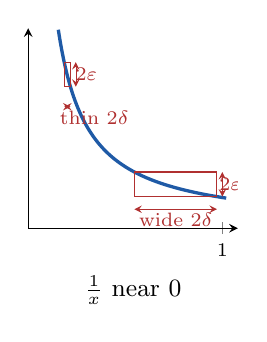
\begin{tikzpicture}
\begin{axis}[nfig, width=0.35\textwidth, height=0.34\textwidth,
  xmin=0, xmax=1.08, ymin=0, ymax=6.5, xtick={1}, ytick=\empty, xlabel={$\tfrac1x$ near $0$}]
  \addplot[figB, very thick, domain=0.155:1.02, samples=200] {1/x};
  \draw[figR, thin] (axis cs:0.5469,1.0286) rectangle (axis cs:0.9722,1.8286);
  \draw[figR, thin] (axis cs:0.1852,4.6) rectangle (axis cs:0.2174,5.4);
  \draw[figR, stealth-stealth, very thin] (axis cs:1.00,1.0286) -- (axis cs:1.00,1.8286);
  \node[font=\scriptsize, figR] at (axis cs:1.04,1.43) {$2\varepsilon$};
  \draw[figR, stealth-stealth, very thin] (axis cs:0.245,4.6) -- (axis cs:0.245,5.4);
  \node[font=\scriptsize, figR] at (axis cs:0.30,5.0) {$2\varepsilon$};
  \draw[figR, stealth-stealth, very thin] (axis cs:0.5469,0.62) -- (axis cs:0.9722,0.62);
  \node[font=\scriptsize, figR] at (axis cs:0.76,0.27) {wide $2\delta$};
  \draw[figR, stealth-stealth, very thin] (axis cs:0.1852,3.95) -- (axis cs:0.2174,3.95);
  \node[font=\scriptsize, figR] at (axis cs:0.34,3.6) {thin $2\delta$};
\end{axis}
\end{tikzpicture}\hfill
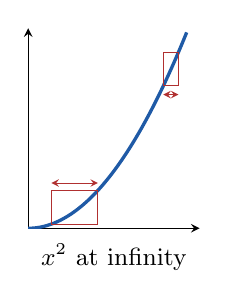
\begin{tikzpicture}
\begin{axis}[nfig, width=0.31\textwidth, height=0.34\textwidth,
  xmin=0, xmax=3.3, ymin=0, ymax=9.5, xtick=\empty, ytick=\empty, xlabel={$x^2$ at infinity}]
  \addplot[figB, very thick, domain=0:3.05, samples=100] {x^2};
  \draw[figR, thin] (axis cs:0.4472,0.2) rectangle (axis cs:1.3416,1.8);
  \draw[figR, thin] (axis cs:2.6005,6.7625) rectangle (axis cs:2.8918,8.3625);
  \draw[figR, stealth-stealth, very thin] (axis cs:0.4472,2.15) -- (axis cs:1.3416,2.15);
  \draw[figR, stealth-stealth, very thin] (axis cs:2.6005,6.35) -- (axis cs:2.8918,6.35);
\end{axis}
\end{tikzpicture}\hfill
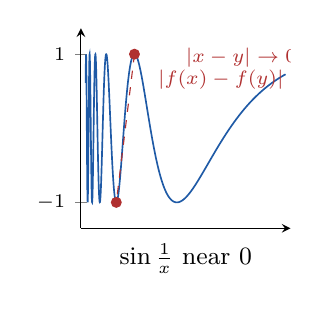
\begin{tikzpicture}
\begin{axis}[nfig, width=0.35\textwidth, height=0.34\textwidth,
  xmin=0.02, xmax=0.44, ymin=-1.35, ymax=1.35, xtick=\empty, ytick={-1,1},
  yticklabels={$-1$,$1$}, xlabel={$\sin\tfrac1x$ near $0$}]
  \addplot[figB, domain=0.0295:0.43, samples=1600, line width=0.6pt] {sin(deg(1/x))};
  \draw[figR, dashed, thin] (axis cs:0.1273,1) -- (axis cs:0.0909,-1);
  \addplot[only marks, mark=*, mark size=1.5pt, figR] coordinates {(0.1273,1) (0.0909,-1)};
  \node[font=\scriptsize, figR, align=center, anchor=west] at (axis cs:0.155,0.80)
    {$|x - y| \to 0$\\ $|f(x) - f(y)| = 2$};
\end{axis}
\end{tikzpicture}\figcap{The three ways uniform continuity fails. Left: $\tfrac1x$ is steep near $0$ --- boxes of the \emph{same} height $2\varepsilon$, fitted so the curve exits through their sides, must get thinner and thinner: no single $\delta$ serves all points. Middle: $x^2$ has the same disease at infinity. Right: $\sin\tfrac1x$ is bounded, but adjacent peak and trough get arbitrarily close horizontally while staying $2$ apart vertically.}
\end{center}


\subsection{Continuity on Closed Intervals Implies Uniform Continuity}

\begin{thmbox}[Uniform Continuity on Closed Bounded Intervals]
If $f: [a,b] \to \mathbb{R}$ is a continuous function on a closed bounded interval, then $f$ is uniformly continuous.
\end{thmbox}

This is another important property of continuous functions on closed bounded intervals --- crucial for the Riemann integral $\int_a^b f(x)\,dx$ later.

\begin{proof}
It is not clear how to produce a uniform $\delta$ directly, so we prove it by contradiction. If $f$ is not uniformly continuous, there exists $\varepsilon > 0$ such that for every $\delta = \tfrac1n$, $n \in \mathbb{N}$, there is a pair $x_n, y_n \in [a,b]$ with
\[
|x_n - y_n| < \frac1n \qquad \text{but} \qquad |f(x_n) - f(y_n)| \geq \varepsilon.
\]
Since $x_n \in [a,b]$ is a bounded sequence, Bolzano--Weierstrass gives a convergent subsequence $x_{n_k} \to x_0$, and $x_0 \in [a,b]$ (limits preserve the endpoint inequalities). Then also $y_{n_k} \to x_0$ --- why? --- because
\[
|y_{n_k} - x_0| \leq |y_{n_k} - x_{n_k}| + |x_{n_k} - x_0| < \frac{1}{n_k} + |x_{n_k} - x_0| \longrightarrow 0.
\]
Since $f$ is continuous at $x_0$: $f(x_{n_k}) \to f(x_0)$ and $f(y_{n_k}) \to f(x_0)$, so
\[
|f(x_{n_k}) - f(y_{n_k})| \longrightarrow 0,
\]
contradicting $|f(x_n) - f(y_n)| \geq \varepsilon$ for all $n$.
\end{proof}

\begin{rembox}[Why should this be true?]
Giving a proof is not enough --- like driving, you need to \emph{feel} it. Here is the suggestive (non-rigorous) picture. Continuity provides, at each point $x_0$, a quantity $\delta = \delta(\varepsilon, x_0) > 0$. The choice is not unique, and it seems reasonable that a ``suitable'' choice is \emph{continuous} in $x_0$. But a continuous positive function on $[a,b]$ attains a \emph{minimum} (Extreme Value Theorem), which is then positive --- and this worst-case value serves as the uniform $\delta$. \textbf{This is not a proof} --- but it explains the theorem, and the actual proof mirrors it: assuming failure, we hunt down the ``bad places'' with Bolzano--Weierstrass, just as in the proof of the Extreme Value Theorem itself. Bolzano--Weierstrass is the basis of many results --- that is why it is so important.
\end{rembox}

\subsection{Uniform Continuity and Cauchy Sequences}

\begin{exbox}[Steepness at infinity (HW)]
The closed-interval theorem needs \emph{both} hypotheses: bounded is as essential as closed. On the closed but unbounded set $\mathbb{R}$, even the polynomial $f(x) = x^3$ fails to be uniformly continuous. Following the negation format above, take the pairs
\[
x_n = n, \qquad y_n = n + \frac1n: \qquad |y_n - x_n| = \frac1n \to 0,
\]
but
\[
|f(y_n) - f(x_n)| = \left( n + \tfrac1n \right)^3 - n^3 = 3n + \frac{3}{n} + \frac{1}{n^3} \geq 3.
\]
So for $\varepsilon_0 = 3$, no $\delta$ can work. Compare the reciprocal example: there the failure was steepness \emph{near $0$} on a bounded set; here it is steepness \emph{at infinity} on a closed set. (On any $[-M, M]$, of course, $x^3$ is uniformly continuous by the theorem.) \hfill $\blacksquare$
\end{exbox}

\begin{propbox}[Uniform Continuity via Continuous Extension (HW)]
Trivially, if $f$ is uniformly continuous on a set $A$, it is uniformly continuous on every subset of $A$ (the same $\delta$ works). Combining with the theorem: if $f: (a, b] \to \mathbb{R}$ extends to a \emph{continuous} function $\tilde f: [a,b] \to \mathbb{R}$, then $f$ is uniformly continuous on $(a,b]$.
\end{propbox}

\begin{proof}
$\tilde f$ is continuous on the finite closed interval $[a,b]$, hence uniformly continuous there by the theorem; and $f = \tilde f$ on the subset $(a,b]$.
\end{proof}

\begin{exbox}[Extension versus oscillation (HW)]
\textbf{(1)} $f(x) = x^2 \sin\tfrac1x$ \emph{is} uniformly continuous on $(0,1]$. Extend by $\tilde f(0) = 0$: continuity at $0$ holds since $|\tilde f(x) - \tilde f(0)| = |x^2 \sin\tfrac1x| \leq x^2$, so $\delta = \sqrt\varepsilon$ works ($\S 17$'s squeeze); on $(0,1]$, $\tilde f = f$ is continuous by the product and composition theorems. Apply the proposition.

\textbf{(2)} By contrast, $g(x) = \sin\tfrac{1}{x^2}$ is \emph{not} uniformly continuous on $(0,1]$, although it is bounded and the set is bounded --- a third failure mode: \emph{oscillation}. Take the pairs
\[
x_n = \frac{1}{\sqrt{2\pi n}}, \qquad y_n = \frac{1}{\sqrt{2\pi n + \tfrac\pi2}}:
\qquad g(x_n) = \sin(2\pi n) = 0, \quad g(y_n) = \sin\left(2\pi n + \tfrac\pi2\right) = 1,
\]
so $|g(x_n) - g(y_n)| = 1$, while $|x_n - y_n| \leq x_n \to 0$. No continuous extension to $[0,1]$ can exist for this $g$ --- and in fact the converse of the proposition is also true (Ross 19.5): a uniformly continuous function on $(a,b]$ \emph{always} extends continuously to $[a,b]$, essentially by the Cauchy-preservation theorem below. Extension and uniform continuity are two descriptions of the same phenomenon. \hfill $\blacksquare$
\end{exbox}

\begin{thmbox}[Uniformly Continuous Functions Preserve Cauchy Sequences]
If $f: \Omega \to \mathbb{R}$ is uniformly continuous and $(s_n)$ is a Cauchy sequence in $\Omega$, then $(f(s_n))$ is also a Cauchy sequence.
\end{thmbox}

\begin{proof}
Given $\varepsilon > 0$, we need $N$ such that $|f(s_n) - f(s_m)| < \varepsilon$ for all $m, n \geq N$. Uniform continuity provides $\delta = \delta(\varepsilon) > 0$ such that $|x - y| < \delta$ implies $|f(x) - f(y)| < \varepsilon$ for $x, y \in \Omega$. Since $(s_n)$ is Cauchy, applied with tolerance $\delta$: there exists $N$ such that $|s_n - s_m| < \delta$ for $m, n \geq N$. For such $m, n$: $|f(s_n) - f(s_m)| < \varepsilon$. Done.
\end{proof}

\begin{rembox}[Warning with counterexample]
If $f$ is only continuous but not uniformly continuous, the conclusion fails. To build a counterexample, start from our non-uniformly continuous function $f(x) = \tfrac1x$ on $(0,+\infty)$. Which Cauchy sequence to take? The problem with $f$ is near $0$, so take $s_n \to 0$: say $s_n = \tfrac1n$ --- Cauchy, since convergent. But
\[
f(s_n) = n,
\]
not Cauchy at all (unbounded).
\end{rembox}

\begin{propbox}[Uniformly Continuous on a Bounded Set Implies Bounded]
Let $\Omega \subseteq \mathbb{R}$ be a bounded set. If $f: \Omega \to \mathbb{R}$ is uniformly continuous, then $f$ is bounded. (An important case: $\Omega = (a,b)$. Without uniform continuity this fails: $f(x) = \tfrac1x$ on $(0,1)$.)
\end{propbox}

\begin{proof}
If not, then for every $n \in \mathbb{N}$ there is $x_n \in \Omega$ with $|f(x_n)| \geq n$. Since $\Omega$ is bounded, $(x_n)$ is a bounded sequence; by Bolzano--Weierstrass there is a convergent subsequence $x_{n_k} \to x_0$. Now $x_0$ \emph{may not belong to $\Omega$} --- this is exactly why we cannot argue with continuity at $x_0$, and why the Cauchy theorem above is the right tool: $(x_{n_k})$, being convergent, is a Cauchy sequence in $\Omega$, so $(f(x_{n_k}))$ is Cauchy, hence convergent, hence \emph{bounded} (\S 10, \S 9). But $|f(x_{n_k})| \geq n_k \to \infty$ --- a contradiction.
\end{proof}

\subsection{A Criterion via the Derivative}

\begin{thmbox}[Bounded Derivative Implies Uniform Continuity]
Let $f: (a, +\infty) \to \mathbb{R}$ be continuous. If $f$ is differentiable with bounded derivative --- $|f'(x)| \leq M$ for all $x$ --- then $f$ is uniformly continuous. The same holds on any interval $(a,b)$, $(a,b]$, $[a,b)$ with $f$ differentiable and $f'$ bounded on the interior.
\end{thmbox}

\begin{proof}
We need the \textbf{Mean Value Theorem}, which we accept now and prove later (Part II). For any pair $x, y$ in the interval, the MVT gives a point $c$ between them with
\[
f(x) - f(y) = f'(c)(x - y), \qquad \text{hence} \qquad |f(x) - f(y)| = |f'(c)|\,|x-y| \leq M |x - y|
\]
--- a simple bound in terms of $|x-y|$. So for every $\varepsilon > 0$, take $\delta = \varepsilon / M$: when $|x - y| < \delta$, $|f(x) - f(y)| \leq M|x-y| < \varepsilon$. Done.
\end{proof}

\begin{exbox}[Cosine]
$f(x) = \cos x: \mathbb{R} \to \mathbb{R}$ is uniformly continuous: $f'(x) = -\sin x$ is bounded by $1$. (As before, $\sin$, $\cos$ and their derivatives are used on credit here.)
\end{exbox}

\begin{rembox}[The converse fails]
A uniformly continuous differentiable function need not have bounded derivative. Take $f(x) = \sqrt{x}$ on $[0,1]$: it is continuous on the closed bounded interval, hence uniformly continuous there (theorem above) --- and therefore also uniformly continuous on the open interval $(0,1)$. But
\[
f'(x) = \frac{1}{2\sqrt x}, \qquad x \in (0,1),
\]
is not bounded.
\end{rembox}

So each of the two theorems covers a region the other misses: near $0$, the closed-interval theorem handles $\sqrt x$ (steep but compact); far out, the derivative $\tfrac{1}{2\sqrt x} \leq \tfrac12$ is bounded on $[1, \infty)$ (HW). Can the two regions be \emph{glued}?

\begin{propbox}[Gluing Lemma for Uniform Continuity (HW)]
Let $c \in \mathbb{R}$ and let $f$ be uniformly continuous on $A = (-\infty \text{ or } a, c]$ and on $B = [c, b \text{ or } \infty)$. Then $f$ is uniformly continuous on $A \cup B$. The junction point must belong to \emph{both} pieces.
\end{propbox}

\begin{proof}
Given $\varepsilon > 0$, uniform continuity on $A$ and on $B$ provides $\delta_A, \delta_B > 0$ for the tolerance $\tfrac\varepsilon2$; take $\delta = \min\{\delta_A, \delta_B\}$. Let $x, y \in A \cup B$ with $|x - y| < \delta$, say $x \leq y$. If both lie in the same piece, then $|f(x) - f(y)| < \tfrac\varepsilon2 < \varepsilon$ directly. Otherwise $x \leq c \leq y$, and the junction point mediates: $|x - c| \leq |x - y| < \delta$ and $|c - y| \leq |x-y| < \delta$, with the pairs $(x, c)$ and $(c, y)$ each inside one piece, so
\[
|f(x) - f(y)| \leq |f(x) - f(c)| + |f(c) - f(y)| < \frac\varepsilon2 + \frac\varepsilon2 = \varepsilon. \qedhere
\]
\end{proof}

\begin{exbox}[The square root globally]
$f(x) = \sqrt x$ is uniformly continuous on all of $[0, +\infty)$: on $[0,1]$ by the closed-interval theorem, on $[1, +\infty)$ by the bounded-derivative theorem, and on the union by the gluing lemma with $c = 1$. Each of the three results of this section contributes exactly the step the others cannot supply. \hfill $\blacksquare$
\end{exbox}

% ============================================================================
% SECTION 20: LIMITS OF FUNCTIONS
% ============================================================================

\section{Limits of Functions}

Recall: $f$ is continuous at $x_0$ if $x_n \to x_0$ implies $f(x_n) \to f(x_0)$. What we \emph{really} want to say is: as $x \to x_0$, $f(x) \to f(x_0)$ --- with the continuous variable $x$, not just discrete sequences. This jump from discrete to continuous is an important interplay in mathematics and science; we now formalize it.

\begin{defbox}[Limit of a Function Along a Set]
Let $S \subseteq \mathbb{R}$, let $a \in [-\infty, +\infty]$ be the limit of some sequence in $S$ (in the terminology of \S 13: $a$ lies in the closure of $S$, allowing $\pm\infty$), and let $L \in [-\infty, +\infty]$. Given $f: S \to \mathbb{R}$, we say \textbf{$f(x) \to L$ as $x \to a$ through $S$}, written
\[
\lim_{x \to a^S} f(x) = L,
\]
if for every sequence $x_n \in S$ with $x_n \to a$, we have $f(x_n) \to L$. The set $S$ controls where the sequence can take its values. Note that $f$ need not be defined at $a$ --- we are \emph{not} comparing $f(x)$ with any value $f(a)$.
\end{defbox}

\begin{rembox}[The epsilon-delta version]
For finite $a$ and $L$, equivalently: for every $\varepsilon > 0$ there exists $\delta > 0$ such that for every $x \in S$ with $|x - a| < \delta$ (and, when $a \notin S$ is intended, $x \neq a$ automatically since $f$ is only defined on $S$),
\[
|f(x) - L| < \varepsilon.
\]
(The equivalence is proved exactly as in \S 17.) If $a = +\infty$, modify: for every $\varepsilon > 0$ there exists $M > 0$ such that $x > M$ implies $|f(x) - L| < \varepsilon$; similarly for $a = -\infty$, and for $L = \pm\infty$ (replace the conclusion by $f(x) > M'$, etc.).
\end{rembox}

\begin{exbox}[First computations]
$S = (0,1)$, $f(x) = \tfrac1x$: then $\lim_{x\to 0^S} f(x) = +\infty$ and $\lim_{x \to 1^S} f(x) = 1$.
\end{exbox}

\begin{thmbox}[Continuity in Terms of Limits]
If $a \in S$, then $f$ is continuous at $a$ if and only if $\lim_{x\to a^S} f(x)$ exists and
\[
\lim_{x \to a^S} f(x) = f(a).
\]
\end{thmbox}

\begin{proof}
Immediate from the sequential definitions of both sides. This is consistent with the intuition: continuity at $a$ means the values of $f(x)$ approach $f(a)$ as $x \to a$.
\end{proof}

\subsection{Notation: Two-Sided and One-Sided Limits}

The notation $\lim_{x\to a^S}$ is a bit inconvenient; in common situations we simplify it:

\begin{defbox}[Standard Limit Notations]
\begin{itemize}
    \item If $S = (c,d) \setminus \{a\}$ with $a \in (c,d)$ (a punctured interval), write $\displaystyle\lim_{x\to a} f(x) = L$ --- the \textbf{two-sided limit}; $S$ is dropped.
    \item If $S = (a, b)$ (points to the right of $a$), write $\displaystyle\lim_{x\to a^+} f(x) = L$: the \textbf{right-hand limit} --- $x > a$ approaching $a$.
    \item If $S = (c, a)$, write $\displaystyle\lim_{x\to a^-} f(x) = L$: the \textbf{left-hand limit}.
    \item If $S = (c, +\infty)$, write $\displaystyle\lim_{x\to+\infty} f(x) = L$; similarly $\displaystyle\lim_{x\to-\infty} f(x) = L$ for $S = (-\infty, c)$.
\end{itemize}
\end{defbox}

Why do we need one-sided limits?

\begin{exbox}[A step function]
Let $f(x) = 1$ for $x > 0$ and $f(x) = 0$ for $x \leq 0$. Is $f$ continuous? No --- not at $0$: the sequence $\tfrac1n \to 0$ has $f(\tfrac1n) = 1 \not\to 0 = f(0)$. Here
\[
\lim_{x\to 0^-} f(x) = 0, \qquad \lim_{x\to 0^+} f(x) = 1, \qquad \lim_{x\to 0} f(x) \ \text{does not exist}
\]
--- we only have the partial limits, from the left and from the right.
\end{exbox}

\begin{exbox}[The reciprocal at its four ends]
For $f(x) = \tfrac1x$ on $S = \mathbb{R}\setminus\{0\}$:
\[
\lim_{x\to+\infty} \frac1x = 0, \qquad \lim_{x\to-\infty} \frac1x = 0, \qquad \lim_{x\to 0^+} \frac1x = +\infty, \qquad \lim_{x\to 0^-} \frac1x = -\infty.
\]
In particular $\lim_{x\to 0} \tfrac1x$ does not exist (not even in $[-\infty,+\infty]$: the one-sided limits differ).
\end{exbox}

\begin{thmbox}[Two-Sided Equals Both One-Sided]
$\displaystyle\lim_{x\to a} f(x) = L$ if and only if
\[
\lim_{x\to a^+} f(x) = L \quad \text{and} \quad \lim_{x\to a^-} f(x) = L.
\]
\end{thmbox}

\begin{proof}
($\Rightarrow$) Clear: a sequence approaching $a$ from within $(a,d)$ (or $(c,a)$) is in particular a sequence in the punctured interval, so the one-sided limits exist and equal $L$.

($\Leftarrow$) Use the $(\varepsilon,\delta)$ formulations. Given $\varepsilon > 0$: from the right-hand limit, there is $\delta_+ > 0$ such that $x > a$, $|x - a| < \delta_+$ imply $|f(x) - L| < \varepsilon$; from the left-hand limit, there is $\delta_- > 0$ such that $x < a$, $|x-a| < \delta_-$ imply $|f(x) - L| < \varepsilon$. Take
\[
\delta = \min\{\delta_+, \delta_-\}:
\]
for every $x$ in the punctured interval with $|x - a| < \delta$, whichever side $x$ is on, $|f(x) - L| < \varepsilon$.
\end{proof}

\begin{rembox}
The usual limit theorems (sums, products, quotients) hold for these limits --- including the one-sided versions --- by the corresponding theorems for sequences; likewise a composition theorem, where one should be careful about matching sides and domains.
\end{rembox}

\subsection{Filling Removable Holes}

These notions can be used to \emph{produce} continuous functions: extend a function to a missing point by its limit there --- when the limit exists.

\begin{exbox}[A removable singularity]
Let $S = \mathbb{R}\setminus\{0\}$ and $f(x) = \dfrac{\sqrt{1+2x^2} - 1}{x^2}$. Can we define $f(0)$ so that $f$ becomes continuous on $\mathbb{R}$? Compute the limit at $0$ by the conjugate:
\[
\frac{\sqrt{1+2x^2}-1}{x^2}
= \frac{(1 + 2x^2) - 1}{x^2\left(\sqrt{1+2x^2}+1\right)}
= \frac{2x^2}{x^2\left(\sqrt{1+2x^2}+1\right)}
= \frac{2}{\sqrt{1+2x^2}+1} \longrightarrow \frac{2}{1+1} = 1.
\]
So $\lim_{x\to0} f(x) = 1$; defining $f(0) = 1$ yields a continuous function on $\mathbb{R}$. \hfill $\blacksquare$
\end{exbox}

\begin{exbox}[A jump that cannot be removed]
Now $g(x) = \dfrac{\sqrt{1 + 2|x|} - 1}{x}$ on $\mathbb{R}\setminus\{0\}$ --- a bit different. The same conjugate computation gives
\[
g(x) = \frac{2|x|}{x\left(\sqrt{1+2|x|}+1\right)},
\]
and $\tfrac{|x|}{x} = \pm1$ depending on the side:
\[
\lim_{x\to 0^+} g(x) = \frac{2}{1+1} = 1, \qquad \lim_{x\to0^-} g(x) = -1.
\]
The one-sided limits differ, so $\lim_{x\to0} g(x)$ does not exist, and \emph{no} value $g(0)$ makes $g$ continuous.
\end{exbox}

\begin{rembox}[Worse than a jump]
For $f(x) = \sin\tfrac1x$, $x \neq 0$: not only does $\lim_{x\to0} f(x)$ not exist --- the left and right limits do not exist either (the oscillation argument of \S 17 works from each side). This is much worse than the previous example: the existence of one-sided limits is already a good property of a function.
\end{rembox}

% ============================================================================
% SECTION 21: MORE ON METRIC SPACES: CONTINUITY
% ============================================================================

\section{More on Metric Spaces: Continuity}

The next two sections generalize what we have learned to metric spaces. (They are important, but discussing them in full would take many lectures; the lecture touched only the key definitions and one theorem.)

\begin{defbox}[Continuous Maps Between Metric Spaces]
Let $(X, d_X)$ and $(Y, d_Y)$ be metric spaces. A map $f: X \to Y$ is \textbf{continuous at $x_0 \in X$} if for every $\varepsilon > 0$ there exists $\delta > 0$ such that for every $x \in X$,
\[
d_X(x, x_0) < \delta \quad \Longrightarrow \quad d_Y\bigl(f(x), f(x_0)\bigr) < \varepsilon.
\]
\end{defbox}

Taking $X = \mathbb{R}$ (or $\Omega \subseteq \mathbb{R}$) and $Y = \mathbb{R}$ with $d(x,y) = |x-y|$ recovers the earlier notion --- the metric-space version is a simple generalization, with each absolute value replaced by the appropriate distance.

% ============================================================================
% SECTION 22: MORE ON METRIC SPACES: CONNECTEDNESS
% ============================================================================

\section{More on Metric Spaces: Connectedness}

Given a subset $S \subseteq \mathbb{R}$, when should we consider it \emph{connected}? Intervals --- $(a,b)$, $[a,b]$, $(a,b]$, $[a,b)$ --- should count: they are like unbroken strings, and we can travel from any point to any other continuously. How about $\mathbb{Q}$? Probably not: we cannot move continuously from one rational to another without leaving $\mathbb{Q}$. There are several ways to make this precise; here is one.

\begin{defbox}[Path-Connected]
A metric space $(X,d)$ is called \textbf{path-connected} if for every two points $x, y \in X$ there exists a continuous map
\[
f: [0,1] \to X \qquad \text{with} \qquad f(0) = x, \quad f(1) = y
\]
--- a continuous, unbroken path from $x$ to $y$.
\end{defbox}

\begin{propbox}[The Rationals Are Not Path-Connected]
$\mathbb{Q}$ (with the metric from $\mathbb{R}$) is not path-connected. In fact, every continuous map $f: [0,1] \to \mathbb{Q}$ is constant.
\end{propbox}

\begin{proof}
View $f$ as a continuous map $[0,1] \to \mathbb{R}$ whose image happens to lie in $\mathbb{Q}$. By the corollary of \S 18, $f([0,1])$ is a closed bounded interval. But which closed intervals are contained in $\mathbb{Q}$? Only the degenerate ones $[c,c] = \{c\}$: any interval with more than one point contains irrationals (density, \S 17). So $f$ is constant --- and no path can join two \emph{distinct} rational numbers.
\end{proof}

% ============================================================================
% CHAPTER 4: SEQUENCES AND SERIES OF FUNCTIONS
% ============================================================================

\chapter{Sequences and Series of Functions}

The idea of this chapter: complicated functions can be built up from simple ones. We need to understand how simple functions can \emph{approximate} and \emph{converge to} complicated functions --- so we need sequences and series of functions, and their notions of convergence.

% ============================================================================
% SECTION 23: POWER SERIES
% ============================================================================

\section{Power Series}

The simplest functions are the constants $a$ and the variable $x$. Starting from them we get all polynomials $a_0 + a_1 x + \cdots + a_n x^n$. Letting $n \to +\infty$, we should get \textbf{power series}
\[
a_0 + a_1 x + a_2 x^2 + \cdots = \sum_{n=0}^{\infty} a_n x^n.
\]

We know the value of a polynomial at every $x$. How about a power series? Take $a_n = 1$: what is $\sum_{n=0}^\infty x^n$ at $x = 2$, i.e.\ $\sum 2^n$? Of course $+\infty$ --- in $\mathbb{R}$. (In a strange number system called the $2$-adic numbers, the answer is $-1$; we will not get into $p$-adic numbers.) So to make sense of a power series \emph{as a function}, we must first determine its \textbf{domain}: for which $x$ does the series converge? Then we must study its properties as a function.

\begin{defbox}[Convergence of a Power Series at a Point]
For a power series $\sum_{n=0}^\infty a_n x^n$, the partial sums are now \emph{functions}
\[
s_n(x) = \sum_{k=0}^n a_k x^k.
\]
We say the series \textbf{converges at $x$} if $\lim_{n\to+\infty} s_n(x)$ exists --- i.e.\ if the numerical series $\sum a_n x^n$ converges in the sense of \S 14.
\end{defbox}

\begin{exbox}[Three domains of convergence]
\textbf{(1)} $\sum_{n=0}^\infty x^n$: converges at $x$ iff $|x| < 1$, with
\[
\sum_{n=0}^\infty x^n = \frac{1}{1-x},
\]
computed directly from $s_n(x) = \tfrac{1-x^{n+1}}{1-x}$ (\S 14). Set of convergence: $(-1,1)$.

\textbf{(2)} $\sum_{n=1}^\infty \dfrac{x^n}{n^2}$: no simple formula for $s_n(x)$, but the ratio (or root) test gives convergence for $|x| < 1$ and divergence for $|x| > 1$. At $|x| = 1$ the series is dominated by $\sum \tfrac{1}{n^2}$, so it converges (absolutely) at both $x = 1$ and $x = -1$. Set of convergence: $[-1, 1]$.

\textbf{(3)} $\sum_{n=1}^\infty \dfrac{x^n}{n}$: converges for $|x| < 1$, diverges for $|x| > 1$; at $x = -1$ it is the alternating harmonic series (converges, \S 15), at $x = 1$ the harmonic series (diverges). Set of convergence: $[-1, 1)$.
\end{exbox}

These examples display the general pattern:

\begin{thmbox}[Trichotomy for the Set of Convergence]
For any power series $\sum_{n=0}^\infty a_n x^n$, exactly one of the following holds:
\begin{enumerate}[label=(\arabic*)]
    \item it converges for all $x \in \mathbb{R}$;
    \item it converges only for $x = 0$;
    \item it converges for all $x$ in a bounded interval centered at $0$ --- which can be closed, open, or half-open, as the examples show --- and diverges outside that interval.
\end{enumerate}
\end{thmbox}

\begin{exbox}[The extreme cases]
$\sum_{n=0}^\infty \dfrac{x^n}{n!}$ converges for \emph{all} $x$: by the ratio test at fixed $x$, $\left|\tfrac{a_{n+1}x^{n+1}}{a_n x^n}\right| = \tfrac{|x|}{n+1} \to 0 < 1$ (this is $\sum \tfrac{|x|^n}{n!}$-type convergence from \S 9). $\sum_{n=0}^\infty n!\, x^n$ converges \emph{only} for $x = 0$: for $x \neq 0$, $(n!)^{1/n} \to +\infty$, so $\limsup |n! x^n|^{1/n} = +\infty > 1$ and the root test gives divergence.
\end{exbox}

The precise version of the trichotomy:

\begin{thmbox}[Radius of Convergence]
For a power series $\sum_{n=0}^\infty a_n x^n$, let
\[
\beta = \limsup_{n\to+\infty} |a_n|^{1/n}, \qquad R = \frac{1}{\beta}
\]
(with the conventions $R = +\infty$ if $\beta = 0$, and $R = 0$ if $\beta = +\infty$). Then:
\begin{enumerate}[label=(\arabic*)]
    \item the series converges (absolutely) for all $|x| < R$;
    \item it diverges for all $|x| > R$.
\end{enumerate}
If $R = 0$, it converges only at $x = 0$; if $R = +\infty$, for all $x$. At $|x| = R$ (when $0 < R < \infty$), extra work is needed case by case. $R$ is called the \textbf{radius of convergence}.
\end{thmbox}

\begin{proof}
Apply the root test (\S 14) to the series $\sum a_n x^n$ at fixed $x$:
\[
\limsup_{n\to+\infty} |a_n x^n|^{1/n} = |x| \limsup_{n\to+\infty} |a_n|^{1/n} = |x| \beta,
\]
using that a nonnegative constant factor passes through the $\limsup$ ($\limsup (c\, b_n) = c \limsup b_n$ for $c \geq 0$ --- from the corresponding fact for tail-sups). The root test gives absolute convergence when $|x|\beta < 1$, i.e.\ $|x| < R$, and divergence when $|x|\beta > 1$, i.e.\ $|x| > R$; the conventions handle $\beta = 0, +\infty$.
\end{proof}

\begin{rembox}
The nice thing: a simple pattern. The domain of convergence of a power series is always an interval, determined by the single number $R$ --- only the endpoint behavior needs individual attention.
\end{rembox}

\subsection{Worked Examples on the Radius}

\begin{exbox}[Integer coefficients]
Assume all $a_n$ are integers and infinitely many are nonzero. Prove $R \leq 1$.

The nonzero coefficients form a subsequence $a_{n_k} \neq 0$ with $|a_{n_k}| \geq 1$ (nonzero integers). \emph{Claim: if the series converges at $x$, then $|x| < 1$.} Indeed, convergence forces $a_n x^n \to 0$ (\S 14), hence along the subsequence $a_{n_k} x^{n_k} \to 0$; but
\[
|a_{n_k} x^{n_k}| \geq |x|^{n_k},
\]
so $|x|^{n_k} \to 0$, which requires $|x| < 1$ (for $|x| \geq 1$, $|x|^{n_k} \geq 1$).

Therefore $R \leq 1$: otherwise $R > 1$ would put $x = 1$ inside $(-R, R)$, forcing convergence at $x = 1$ --- contradicting the claim. (More directly: convergence at $x = 1$ would give $a_n \to 0$, impossible for integers with infinitely many nonzero terms, since $|a_{n_k}| \geq 1$.) \hfill $\blacksquare$
\end{exbox}

\begin{exbox}[Coefficients not tending to zero]
If $\limsup_{n\to+\infty} |a_n| > 0$, prove $R \leq 1$. By contradiction: if $R > 1$, the series converges at $x = 1$, so $a_n = a_n \cdot 1^n \to 0$, hence $|a_n| \to 0$ and $\limsup |a_n| = 0$ --- contradiction. \hfill $\blacksquare$
\end{exbox}

\begin{exbox}[Nonnegative coefficients and endpoints]
Suppose $\sum a_n x^n$ has finite radius $R$ and $a_n \geq 0$ for all $n$. Prove: if the series converges at $x = R$, then it also converges at $x = -R$ --- so the interval of convergence is all of $[-R, R]$.

\emph{Proof.} Convergence at $x = R$ with $a_n \geq 0$ means $\sum a_n R^n$ converges --- and this is exactly $\sum |a_n(-R)^n|$. So the series at $x = -R$ converges \emph{absolutely}, hence converges. \hfill $\blacksquare$

Consequently, an interval of convergence like $(-1, 1]$ requires coefficients of mixed sign. Example:
\[
\sum_{n=1}^\infty (-1)^n \frac{x^n}{n}: \qquad R = 1; \quad \text{at } x = 1: \ \textstyle\sum(-1)^n\frac1n \text{ converges}; \quad \text{at } x = -1: \ \textstyle\sum \frac1n \text{ diverges}.
\]
\end{exbox}

\subsection{Power Series Centered at a Point}

More generally, consider
\[
\sum_{n=0}^{\infty} a_n (x - x_0)^n.
\]
The interval of convergence is now centered at $x_0$: it is $(x_0 - R,\, x_0 + R)$ (with the endpoint questions as before), where $R = 1/\beta$, $\beta = \limsup |a_n|^{1/n}$, exactly as before. The proof is the same root-test computation:
\[
\limsup_{n\to\infty} |a_n (x-x_0)^n|^{1/n} = \beta\, |x - x_0|,
\]
compared with $1$.

\begin{exbox}[Two centered examples]
\textbf{(1)} $\sum_{n=0}^\infty n^2 (x-1)^n$: here $\beta = \lim (n^2)^{1/n} = \left(n^{1/n}\right)^2 \to 1$, so $R = 1$ and the interval is $(0, 2)$. The endpoints $0, 2$ are \emph{not} included: there the terms are $\pm n^2$, which do not tend to $0$, so $\sum n^2(\pm1)^n$ diverges.

\textbf{(2)} $\sum_{n=1}^\infty \left( \dfrac{x-2}{n} \right)^n$: here $a_n = \tfrac{1}{n^n}$, $\beta = \lim \tfrac1n = 0$, $R = +\infty$ --- the series converges for all $x \in \mathbb{R}$.
\end{exbox}

\begin{rembox}[Why centered series? Taylor series]
The main source of centered power series is the \textbf{Taylor series} of a function $f$ at a point $x_0$:
\[
\sum_{n=0}^\infty \frac{f^{(n)}(x_0)}{n!} (x - x_0)^n,
\]
which for $x_0 = 0$ specializes to $\sum \tfrac{f^{(n)}(0)}{n!} x^n$ --- e.g., for $f(x) = e^x$, the series $\sum_{n=0}^\infty \tfrac{x^n}{n!}$, whose radius we computed to be $+\infty$. (This is a preview: derivatives, and the sense in which $e^x$ \emph{equals} its Taylor series, belong to Part II.)
\end{rembox}

\begin{exbox}[Root test beats ratio test]
Let $a_n = \left( \dfrac{3 + 2(-1)^n}{4} \right)^n$ --- that is, $a_n = \left(\tfrac54\right)^n$ for even $n$ and $\left(\tfrac14\right)^n$ for odd $n$. Determine the intervals of convergence of (1) $\sum a_n x^n$ and (2) $\sum a_n (x-2)^n$.

Here $|a_n|^{1/n} = \tfrac{3+2(-1)^n}{4}$ oscillates between $\tfrac54$ and $\tfrac14$, so
\[
\beta = \limsup_{n\to\infty} |a_n|^{1/n} = \frac54, \qquad R = \frac45.
\]
(The \emph{ratio} test is useless here: consecutive ratios swing between roughly $\left(\tfrac14\right)^{n+1}/\left(\tfrac54\right)^n \to 0$ and $\left(\tfrac54\right)^{n+1}/\left(\tfrac14\right)^n \to \infty$, so $\liminf < 1 < \limsup$ --- no information. This example shows the difference in power between the two tests.)

So (1) has interval $\left(-\tfrac45, \tfrac45\right)$ and (2) has $\left(2 - \tfrac45,\ 2 + \tfrac45\right)$, endpoints excluded in both cases: at the endpoints, $|a_n(x - x_0)^n| = |a_n| \left(\tfrac45\right)^n$ equals $1$ along the even indices, so the terms do not tend to $0$. \hfill $\blacksquare$
\end{exbox}

\begin{rembox}[Mind the absolute values (HW)]
The coefficients above were positive; with \emph{signed} coefficients the radius formula must read $\limsup |a_n|^{1/n}$, absolute values included. Take $a_n = \left( \tfrac{1 + 2(-1)^n}{5} \right)^n$, which is $\left(\tfrac35\right)^n$ for even $n$ but $\left(-\tfrac15\right)^n$ --- \emph{negative} --- for odd $n$. The signed root sequence $a_n^{1/n} = \tfrac{1+2(-1)^n}{5}$ oscillates between $\tfrac35$ and $-\tfrac15$, whereas the sequence the formula wants, $|a_n|^{1/n}$, oscillates between $\tfrac35$ and $\tfrac15$: here the two limsups happen to agree ($\tfrac35$, so $R = \tfrac53$), but the signed liminf $-\tfrac15$ is meaningless for convergence questions --- only the moduli $|a_n(x-x_0)^n|$ enter the comparison with a geometric series in the radius theorem's proof.
\end{rembox}

\begin{rembox}[Gap series (HW)]
A second situation where the coefficient-ratio recipe breaks: series with \emph{gaps}, like
\[
\sum_{n=0}^\infty 2^{-n} x^{3n} \qquad \text{or} \qquad \sum_{n=1}^\infty \frac{3^n}{\sqrt n}\, x^{2n+1}.
\]
As power series $\sum a_m x^m$, most coefficients are \emph{zero} ($a_m = 0$ unless $3 \mid m$, resp.\ $m$ odd), so consecutive ratios $a_{m+1}/a_m$ are undefined or useless. Two correct routes. \textbf{(1) Test the whole terms:} fix $x$ and apply the ratio test to the numerical series --- for the second series,
\[
\left| \frac{3^{n+1} x^{2n+3} / \sqrt{n+1}}{3^{n} x^{2n+1} / \sqrt{n}} \right| = 3|x|^2 \sqrt{\tfrac{n}{n+1}} \longrightarrow 3|x|^2,
\]
giving convergence for $3|x|^2 < 1$, divergence for $3|x|^2 > 1$: so $R = \tfrac{1}{\sqrt3}$ (equivalently, substitute $y = x^2$). \textbf{(2) The root formula survives:} $\limsup |a_m|^{1/m}$ ignores the zero terms --- for the first series, $|a_m|^{1/m} = (2^{-n})^{1/3n} = 2^{-1/3}$ along $m = 3n$ and $0$ elsewhere, so $\beta = 2^{-1/3}$ and $R = 2^{1/3}$. Both intervals turn out open, for different reasons: for the first series the endpoint terms have modulus $|2^{-n} x^{3n}| = 1$ at $x = \pm 2^{1/3}$ (no decay at all); for the second, since $x^{2n+1}$ carries the sign of $x$ uniformly, at $x = \pm\tfrac{1}{\sqrt3}$ every term equals $\pm\tfrac{1}{\sqrt3\,\sqrt n}$ --- a single-signed multiple of the divergent p-series with $p = \tfrac12$, so no alternation comes to the rescue. The limsup formula's indifference to gaps is one more point for the root test.
\end{rembox}

\subsection{Do Limits Preserve Good Properties? A Gallery of Failures}

A power series defines a function $f(x) = \sum a_n x^n$ on its interval of convergence --- the limit of the polynomial partial sums $s_n(x)$, each certainly continuous. \textbf{Question: are limits of sequences of continuous functions continuous?} At the beginning of calculus, people did not ask such questions --- they assumed yes automatically. The general answer is \textbf{no}, and the counterexamples below motivate the next section.

\begin{exbox}[Continuity lost in the limit]
Let $f_n(x) = x^n$ on $[0,1]$. For every $x \in [0,1]$, $f_n(x)$ converges: for $x \in [0,1)$, $|x| < 1$ gives $x^n \to 0$; and $f_n(1) = 1$. So the limit function is
\[
f(x) = 0 \ (0 \leq x < 1), \qquad f(1) = 1
\]
--- \emph{not} continuous, though every $f_n$ is.
\end{exbox}

\begin{exbox}[Powers of sine]
$f_n(x) = (\sin x)^n$, $x \in \mathbb{R}$: find all $x$ where $\lim_n f_n(x)$ exists. If $x \neq k\pi + \tfrac\pi2$ ($k \in \mathbb{Z}$), then $|\sin x| < 1$ and $f_n(x) \to 0$. If $\sin x = 1$ (i.e.\ $x = 2k\pi + \tfrac\pi2$), $f_n(x) \to 1$. If $\sin x = -1$ (i.e.\ $x = (2k+1)\pi + \tfrac\pi2$), $f_n(x) = (-1)^n$ diverges. So the limit function has domain $\mathbb{R} \setminus \{(2k+1)\pi + \tfrac\pi2\}$, equals $0$ except at the points $2k\pi + \tfrac\pi2$ where it equals $1$ --- and is not continuous.
\end{exbox}

\begin{exbox}[Derivatives escape the limit]
Since a limit of continuous functions can fail to be continuous, it certainly can fail to be differentiable. Subtler question: suppose $f_n \to f$ pointwise, all $f_n$ differentiable, \emph{and} $f$ differentiable --- must $f_n' \to f'$? \textbf{Still no.} The idea: even if $f_n$ converges, its rate of change can be wild. Let
\[
f_n(x) = \frac1n \sin nx: \qquad f_n(x) \to 0 \text{ for all } x, \quad \text{so } f \equiv 0, \ f' \equiv 0.
\]
But $f_n'(x) = \cos nx$, whose graph oscillates faster and faster as $n$ grows; e.g.\ at $x = \pi$, $f_n'(\pi) = (-1)^n$ diverges --- certainly not converging to $f'(\pi) = 0$. (One can show $\cos nx$ converges only at the points $x = 2k\pi$.)
\end{exbox}

\begin{exbox}[Integrals escape the limit]
Suppose $f_n(x) \to f(x)$ for all $x \in [a,b]$. Does $\int_a^b f_n \to \int_a^b f$? \textbf{No.} Let
\[
f_n(x) = (n+1)x^n \ \ (0 \leq x < 1), \qquad f_n(1) = 0.
\]
Then $f(x) = 0$ for all $x \in [0,1]$ (for $x < 1$, $(n+1)x^n \to 0$ by the growth scale of \S 9). But
\[
\int_0^1 f_n(x)\,dx = x^{n+1}\Big|_0^1 = 1 \not\longrightarrow 0 = \int_0^1 f(x)\,dx.
\]
The mass of the integral escapes to the endpoint. (Integrals here are used in the familiar calculus sense, on credit as usual.)
\end{exbox}

All these examples show: things are subtle and tricky, and we should be careful. The good news: for the partial sums of power series, most of the difficulties disappear --- but to see why, we need a stronger notion of convergence.

% ============================================================================
% SECTION 24: UNIFORM CONVERGENCE
% ============================================================================

\section{Uniform Convergence}

The problem with the examples above: convergence $f_n(x) \to f(x)$ \emph{at every point separately} is not sufficient. We need something stronger.

\begin{defbox}[Pointwise Convergence]
Let $S \subseteq \mathbb{R}$ and $f_n$ functions defined on $S$. The sequence $(f_n)$ \textbf{converges to $f$ pointwise on $S$} if for every $x \in S$, $f_n(x) \to f(x)$. In $(\varepsilon, N)$ terms: for every $x \in S$ and every $\varepsilon > 0$, there exists $N = N(x)$ such that $|f_n(x) - f(x)| < \varepsilon$ for $n \geq N(x)$ --- the integer $N(x)$ \emph{depends on $x$}. All the examples above are pointwise convergence.
\end{defbox}

\begin{defbox}[Uniform Convergence]
$(f_n)$ \textbf{converges uniformly to $f$ on $S$} if for every $\varepsilon > 0$ there exists $N$ such that for all $n \geq N$ \emph{and all $x \in S$},
\[
|f_n(x) - f(x)| < \varepsilon.
\]
The difference: $N$ is independent of $x$ --- one $N$ works for all points. (Compare the passage from continuity to \emph{uniform} continuity in \S 19: the same quantifier move.)
\end{defbox}

\begin{center}
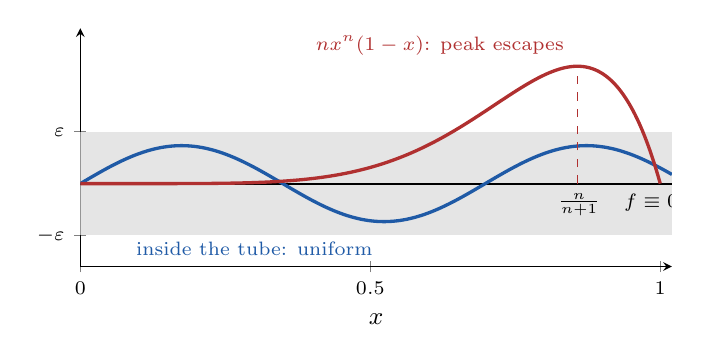
\begin{tikzpicture}
\begin{axis}[nfig, width=0.75\textwidth, height=0.38\textwidth,
  xmin=0, xmax=1.02, ymin=-0.24, ymax=0.45,
  xtick={0,0.5,1}, ytick={-0.15,0.15},
  yticklabels={$-\varepsilon$,$\varepsilon$}, xlabel={$x$}]
  \addplot[draw=none, fill=black!10] coordinates {(0,-0.15) (1.02,-0.15) (1.02,0.15) (0,0.15)};
  \addplot[black, thick, domain=0:1.02] {0} node[pos=0.965, below, font=\scriptsize] {$f\equiv 0$};
  \addplot[figB, very thick, domain=0:1.02, samples=200] {0.11*sin(deg(9*x))};
  \addplot[figR, very thick, domain=0:1, samples=300] {6*x^6*(1-x)};
  \node[figB, font=\scriptsize] at (axis cs:0.30,-0.19) {inside the tube: uniform};
  \node[figR, font=\scriptsize] at (axis cs:0.62,0.40) {$n x^n(1-x)$: peak escapes};
  \draw[figR, dashed, thin] (axis cs:0.857,0) -- (axis cs:0.857,0.34);
  \node[font=\scriptsize] at (axis cs:0.86,-0.06) {$\frac{n}{n+1}$};
\end{axis}
\end{tikzpicture}\figcap{The $\varepsilon$-tube around the limit $f \equiv 0$: uniform convergence means the whole graph of $f_n$ eventually enters the tube. The blue curve is inside; the peak of $n x^n(1-x)$ (height $\to \tfrac1e$ at $x = \tfrac{n}{n+1}$) escapes for every $n$ --- the picture behind ``Locating the worst point'' below.}
\end{center}


\subsection{Examples and Non-Examples}

\begin{exbox}[The geometric series converges pointwise but not uniformly]
Let $f_n(x) = \sum_{k=0}^n x^k = \dfrac{1 - x^{n+1}}{1-x}$ on $S = (-1,1)$. Pointwise, $f_n(x) \to f(x) = \tfrac{1}{1-x}$ for every $x \in S$. But the convergence is \emph{not uniform}.

\emph{Proof.} Suppose it were. Then for every $\varepsilon > 0$ there is $N$ such that for all $n \geq N$ and all $x \in (-1,1)$,
\[
|f_n(x) - f(x)| = \left| \frac{x^{n+1}}{1-x} \right| < \varepsilon, \qquad \text{i.e.} \qquad |x|^{n+1} < \varepsilon\,|1-x|.
\]
Fix any $n \geq N$ and let $x \to 1^-$: the left side tends to $1$, the right side to $0$, giving $1 \leq 0$ --- impossible. \hfill $\blacksquare$

The reason: as $x$ gets close to $1$, the pointwise $N(x)$ blows up, so no uniform $N$ exists.
\end{exbox}

\begin{center}
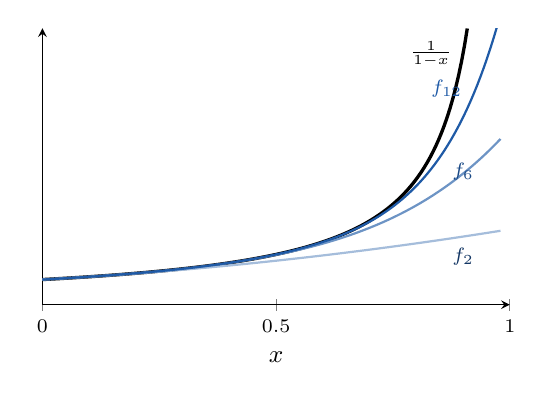
\begin{tikzpicture}
\begin{axis}[nfig, width=0.62\textwidth, height=0.42\textwidth,
  xmin=0, xmax=1.0, ymin=0, ymax=11,
  xtick={0,0.5,1}, ytick=\empty, xlabel={$x$}]
  \addplot[black, very thick, domain=0:0.909, samples=150] {1/(1-x)}
    node[pos=0.90, left, font=\scriptsize] {$\tfrac{1}{1-x}$};
  \addplot[figB!40, thick, domain=0:0.98, samples=100] {(1-x^3)/(1-x)};
  \addplot[figB!65, thick, domain=0:0.98, samples=120] {(1-x^7)/(1-x)};
  \addplot[figB, thick, domain=0:0.98, samples=140] {(1-x^13)/(1-x)};
  \node[font=\scriptsize, figB!60!black] at (axis cs:0.90,1.9) {$f_2$};
  \node[font=\scriptsize, figB!80!black] at (axis cs:0.90,5.3) {$f_6$};
  \node[font=\scriptsize, figB] at (axis cs:0.865,8.6) {$f_{12}$};
\end{axis}
\end{tikzpicture}\figcap{The partial sums peel off near $x = 1$: each $f_n$ eventually flattens (it is a polynomial, bounded on $[0,1]$) while $\tfrac{1}{1-x}$ climbs without bound, so $\sup_x |f_n - f|$ is infinite for every $n$ --- pointwise convergence at each fixed $x$, no uniformity.}
\end{center}


\begin{exbox}[The power sequence on the closed interval]
$f_n(x) = x^n$ on $[0,1]$ converges pointwise to the discontinuous $f$ computed above, but not uniformly. If it did: take $\varepsilon = \tfrac12$; then for $n \geq N$ and all $x \in [0,1)$, $|x^n| < \tfrac12$. Fix $n$ and let $x \to 1^-$: $x^n \to 1$, giving $1 \leq \tfrac12$. Impossible. \hfill $\blacksquare$
\end{exbox}

\begin{exbox}[A uniform example]
$f_n(x) = \tfrac1n \sin x$ converges uniformly to $f \equiv 0$ on $\mathbb{R}$: given $\varepsilon > 0$, take $N > \tfrac1\varepsilon$; then for all $n \geq N$ and \emph{all} $x \in \mathbb{R}$,
\[
|f_n(x) - 0| = \left| \frac{\sin x}{n} \right| \leq \frac1n \leq \frac1N < \varepsilon. \tag*{$\blacksquare$}
\]
\end{exbox}

\begin{exbox}[A two-plateau limit]
Let $f_n(x) = \dfrac{x^n}{n + x^n}$ on $[0, +\infty)$. \emph{Pointwise limit:} for $0 \leq x \leq 1$, $x^n \leq 1$, so for $n \geq 2$, $|f_n(x)| \leq \tfrac1n \to 0$; for $x > 1$, $x^n \to \infty$ faster than $n$ ($n/x^n \to 0$, growth scale), so
\[
f_n(x) = \frac{1}{n/x^n + 1} \longrightarrow \frac{1}{0+1} = 1.
\]
So $f = 0$ on $[0,1]$ and $f = 1$ on $(1,+\infty)$. \emph{Not uniform:} the trouble point is $x = 1$, where $f$ jumps --- a hint. Suppose uniform: for $\varepsilon = \tfrac12$ there is $N$ with, for all $n \geq N$ and all $x > 1$,
\[
|f_n(x) - 1| = \frac{n}{n + x^n} < \frac12.
\]
Fix $n \geq N$ and let $x \to 1^+$: the left side tends to $\tfrac{n}{n+1} \geq \tfrac12$ --- contradiction. \hfill $\blacksquare$
\end{exbox}

\begin{exbox}[Shifted parabolas converge uniformly]
$f_n(x) = \left(x - \tfrac1n\right)^2$ on $[0,1]$: pointwise limit $f(x) = x^2$, and the convergence is uniform --- bound the difference independently of $x$:
\[
|f_n(x) - f(x)| = \left| -\frac{2x}{n} + \frac{1}{n^2} \right| \leq \frac{2x}{n} + \frac{1}{n^2} \leq \frac2n + \frac{1}{n^2} \longrightarrow 0. \tag*{$\blacksquare$}
\]
\end{exbox}

\begin{exbox}[Locating the worst point]
$f_n(x) = n x^n (1-x)$ on $[0,1]$: pointwise, $f \equiv 0$ (for $x \in [0,1)$, $nx^n \to 0$ by the growth scale; $f_n(0) = f_n(1) = 0$). But the convergence is \emph{not} uniform --- harder to prove. We want $\varepsilon_0$ and points $x_n$ (depending on $n$!) with $f_n(x_n) \geq \varepsilon_0$. Which points? \emph{The maximum point of $f_n$ --- the worst case.} Calculus locates it: $f_n'(x) = n^2 x^{n-1} - n(n+1)x^n = 0$ gives $x_n = \tfrac{n}{n+1}$. (The derivative is only a \emph{search tool}; the proof below needs nothing but the evaluation.) Compute:
\[
f_n\left(\frac{n}{n+1}\right) = n \left(\frac{n}{n+1}\right)^n \frac{1}{n+1}
= \frac{n}{n+1} \left(\frac{1}{1 + \tfrac1n}\right)^n
\longrightarrow 1 \cdot \frac1e = \frac1e,
\]
using the standard limit $\left(1 + \tfrac1n\right)^n \to e$ (provable with monotone convergence; accepted here). So taking $\varepsilon_0 = \tfrac{1}{2e}$: for all large $n$,
\[
\left| f_n\left( \tfrac{n}{n+1} \right) - 0 \right| \geq \varepsilon_0,
\]
which rules out uniform convergence. \hfill $\blacksquare$
\end{exbox}

\subsection{The Supremum Criterion}

The last example generalizes:

\begin{thmbox}[Supremum Criterion for Uniform Convergence]
$f_n \to f$ uniformly on $S$ if and only if
\[
\lim_{n\to\infty} M_n = 0, \qquad \text{where} \quad M_n = \sup\{ |f_n(x) - f(x)| \mid x \in S \}.
\]
\end{thmbox}

\begin{proof}
($\Leftarrow$) If $M_n \to 0$: for every $\varepsilon > 0$ there is $N$ with $M_n < \varepsilon$ for $n \geq N$; then for all $x \in S$, $|f_n(x) - f(x)| \leq M_n < \varepsilon$.

($\Rightarrow$) If $f_n \to f$ uniformly: for every $\varepsilon > 0$ there is $N$ such that $|f_n(x) - f(x)| < \varepsilon$ for all $n \geq N$ and all $x \in S$; taking the supremum over $x$, $M_n \leq \varepsilon$ for $n \geq N$. Hence $M_n \to 0$.
\end{proof}

The two proof strategies, summarized: to prove uniform convergence, bound $|f_n(x) - f(x)|$ \emph{independently of $x$} by something $\to 0$; to disprove it, find points $x_n$ (usually depending on $n$) where $|f_n(x_n) - f(x_n)|$ stays above a fixed $\varepsilon_0$.

\subsection{Uniform Limits of Continuous Functions}

Now we reap the applications.

\begin{thmbox}[Uniform Limits Preserve Continuity]
If every $f_n$ is continuous on $S$ and $f_n \to f$ \emph{uniformly} on $S$, then $f$ is continuous on $S$.
\end{thmbox}

\begin{proof}
Fix $x_0 \in S$ and $\varepsilon > 0$; we need $\delta > 0$ such that $|x - x_0| < \delta$ (with $x \in S$) implies $|f(x) - f(x_0)| < \varepsilon$. \emph{Idea: approximate $f$ by one continuous $f_N$.}

By uniform convergence, there exists $N$ such that for all $x \in S$,
\[
|f_N(x) - f(x)| < \frac\varepsilon3.
\]
Since $f_N$ is continuous at $x_0$, there exists $\delta > 0$ such that $|x - x_0| < \delta$, $x \in S$, implies
\[
|f_N(x) - f_N(x_0)| < \frac\varepsilon3.
\]
Now, for such $x$, insert $f_N$ twice:
\[
|f(x) - f(x_0)| \leq \underbrace{|f(x) - f_N(x)|}_{< \varepsilon/3} + \underbrace{|f_N(x) - f_N(x_0)|}_{< \varepsilon/3} + \underbrace{|f_N(x_0) - f(x_0)|}_{< \varepsilon/3} < \varepsilon.
\]
The first and third bounds come from uniform convergence, the middle from continuity of $f_N$ --- exactly the idea of approximation. So $f$ is continuous at $x_0$.
\end{proof}

\begin{rembox}
This retroactively explains several examples: $x^n$ on $[0,1]$ and $\tfrac{x^n}{n+x^n}$ on $[0,\infty)$ could not converge uniformly, because their limit functions are discontinuous while every $f_n$ is continuous. The contrapositive of the theorem is a quick non-uniformity test.
\end{rembox}

Continuity is not the only property that survives passage to a uniform limit:

\begin{propbox}[Uniform Limits Preserve Boundedness (HW)]
If every $f_n$ is bounded on $S$ and $f_n \to f$ uniformly on $S$, then $f$ is bounded on $S$.
\end{propbox}

\begin{proof}
One term of the sequence suffices. By uniform convergence (with tolerance $1$, say) there is $N$ such that $|f_N(x) - f(x)| < 1$ for \emph{all} $x \in S$; and $f_N$ is bounded, say $|f_N| \leq M_N$ on $S$. Then for every $x \in S$,
\[
|f(x)| \leq |f(x) - f_N(x)| + |f_N(x)| < 1 + M_N,
\]
a bound independent of $x$.
\end{proof}

\begin{rembox}
This is the function-space analogue of ``convergent sequences of numbers are bounded'' (\S 9) --- there too, one tail estimate plus one fixed term produced the bound. Uniformity is essential: on $(0,1]$ the truncations $f_n(x) = \min\left\{ n, \tfrac1x \right\}$ are each bounded (by $n$) and converge \emph{pointwise} to $\tfrac1x$, which is unbounded; the convergence cannot be uniform, and the proposition is precisely what forbids it.
\end{rembox}

\begin{exbox}[Products do not preserve uniform convergence (HW)]
Sums do, trivially: if $f_n \to f$ and $g_n \to g$ uniformly on $S$, then $|(f_n + g_n) - (f+g)| \leq |f_n - f| + |g_n - g|$ gives $f_n + g_n \to f + g$ uniformly. But \emph{products fail}. Take on $\mathbb{R}$:
\[
f_n(x) = x, \qquad g_n(x) = \frac1n,
\]
so $f_n \to f(x) = x$ uniformly (the differences are $0$) and $g_n \to g \equiv 0$ uniformly ($|g_n - g| = \tfrac1n$, independent of $x$). Yet $(f_n g_n)(x) = \tfrac{x}{n}$ does not converge uniformly to $fg \equiv 0$: for $\varepsilon_0 = 1$ and any $n$, the point $x = n$ gives $\left|\tfrac{x}{n}\right| = 1$. The culprit is the \emph{unbounded} factor $x$, which amplifies the innocent error $\tfrac1n$ without limit; if $f$, $g$ and all $f_n$, $g_n$ are bounded, the product does converge uniformly (and the proposition above says the limits' boundedness comes for free from the $f_n$'s). \hfill $\blacksquare$
\end{exbox}

% ============================================================================
% SECTION 25: MORE ON UNIFORM CONVERGENCE
% ============================================================================

\section{More on Uniform Convergence}

\subsection{Exchanging Limits and Integrals}

Return to the integral question. Our earlier counterexample $(n+1)x^n$ had a flaw for the refined question: $f_n$ was not continuous at $x = 1$. Could continuity of all $f_n$ \emph{and} of $f$ rescue $\int f_n \to \int f$ under pointwise convergence? Still no:

\begin{exbox}[The escaping triangle]
Define $f_n: [0,1] \to \mathbb{R}$ with a thin tall triangular graph --- base $[0, \tfrac2n]$, height $n$, zero elsewhere:
\[
f_n(x) = n^2 x \ \left(0 \leq x \leq \tfrac1n\right), \qquad
f_n(x) = n^2\left(\tfrac2n - x\right) \ \left(\tfrac1n \leq x \leq \tfrac2n\right), \qquad
f_n(x) = 0 \ \text{ otherwise}.
\]
Each $f_n$ is continuous, and by the area formula for triangles,
\[
\int_0^1 f_n(x)\,dx = \frac12 \cdot \frac2n \cdot n = 1.
\]
But $f(x) = \lim f_n(x) = 0$ for \emph{all} $x \in [0,1]$: for $x > 0$, once $\tfrac2n < x$ the triangle has slid past $x$ and $f_n(x) = 0$; and $f_n(0) = 0$ always. The triangle becomes skinnier and skinnier and escapes. So $\int_0^1 f_n = 1 \not\to 0 = \int_0^1 f$, with all continuity conditions satisfied.
\end{exbox}

\begin{center}
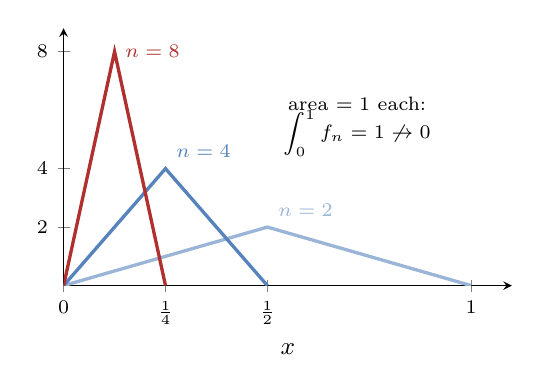
\begin{tikzpicture}
\begin{axis}[nfig, width=0.60\textwidth, height=0.40\textwidth,
  xmin=0, xmax=1.1, ymin=0, ymax=8.8,
  xtick={0,0.25,0.5,1}, xticklabels={$0$,$\tfrac14$,$\tfrac12$,$1$}, ytick={2,4,8}, xlabel={$x$}]
  \addplot[figB!45, very thick] coordinates {(0,0) (0.5,2) (1,0)}
     node[pos=0.5, above right, font=\scriptsize] {$n=2$};
  \addplot[figB!75, very thick] coordinates {(0,0) (0.25,4) (0.5,0)}
     node[pos=0.5, above right, font=\scriptsize] {$n=4$};
  \addplot[figR, very thick] coordinates {(0,0) (0.125,8) (0.25,0)}
     node[pos=0.5, right, font=\scriptsize] {$n=8$};
  \node[font=\scriptsize] at (axis cs:0.72,6.2) {area $=1$ each:};
  \node[font=\scriptsize] at (axis cs:0.72,5.2) {$\displaystyle\int_0^1 f_n = 1 \not\to 0$};
\end{axis}
\end{tikzpicture}\figcap{The escaping triangle for $n = 2, 4, 8$: base $[0, \tfrac2n]$ shrinks, peak $n$ grows, area stays exactly $1$. Pointwise the limit is $0$ everywhere, yet the integrals refuse to follow.}
\end{center}


\begin{thmbox}[Uniform Convergence Allows Exchanging Limit and Integral]
If $f_n \to f$ uniformly on $[a,b]$ (with each $f_n$ continuous, so that $f$ is continuous and all integrals are defined), then
\[
\lim_{n\to\infty} \int_a^b f_n(x)\,dx = \int_a^b f(x)\,dx = \int_a^b \lim_{n\to\infty} f_n(x)\,dx
\]
--- the limit and the integration can be exchanged. This is one of the problems that motivated uniform convergence.
\end{thmbox}

\begin{proof}
Given $\varepsilon > 0$, uniform convergence provides $N$ such that for all $n \geq N$ and all $x \in [a,b]$,
\[
|f_n(x) - f(x)| < \frac{\varepsilon}{b-a}.
\]
Therefore, using the basic bounds $\left|\int g\right| \leq \int |g|$ and monotonicity of the integral (familiar from calculus; rigorous in Part III),
\[
\left| \int_a^b f_n - \int_a^b f \right| = \left| \int_a^b (f_n - f) \right| \leq \int_a^b |f_n - f| \leq \int_a^b \frac{\varepsilon}{b-a}\,dx = \varepsilon. \qedhere
\]
\end{proof}

\begin{exbox}[Computing a limit of integrals]
Compute $\displaystyle\lim_{n\to\infty} \int_0^1 \frac{n + \cos x}{2n + \sin^2 x}\,dx$.

Computing $\int_0^1 f_n$ directly is difficult --- so try exchanging: divide through by $n$,
\[
f_n(x) = \frac{1 + \tfrac{\cos x}{n}}{2 + \tfrac{\sin^2 x}{n}} \longrightarrow \frac12 \qquad \text{for every } x.
\]
To justify the exchange, show the convergence is uniform:
\[
\left| f_n(x) - \frac12 \right|
= \frac{\left| 2\left(1 + \tfrac{\cos x}{n}\right) - \left(2 + \tfrac{\sin^2 x}{n}\right) \right|}{2\left(2 + \tfrac{\sin^2 x}{n}\right)}
= \frac{\left| \tfrac{2\cos x}{n} - \tfrac{\sin^2 x}{n} \right|}{2\left(2 + \tfrac{\sin^2 x}{n}\right)}
\leq \frac{\tfrac2n + \tfrac1n}{4} = \frac{3}{4n},
\]
a bound independent of $x$ tending to $0$. By the supremum criterion the convergence is uniform, and by the theorem,
\[
\lim_{n\to\infty} \int_0^1 f_n(x)\,dx = \int_0^1 \frac12\,dx = \frac12. \tag*{$\blacksquare$}
\]
\end{exbox}

\subsection{Series of Functions and the Weierstrass M-Test}

Now we return toward power series --- via general series of functions.

\begin{defbox}[Convergence of a Series of Functions]
Let $g_k$ be functions defined on a common set $S \subseteq \mathbb{R}$, with partial sums $s_n(x) = \sum_{k=1}^n g_k(x)$. If $s_n(x) \to g(x)$ pointwise on $S$, we say the series $\sum_{k=1}^\infty g_k(x)$ \textbf{converges pointwise} and write $g(x) = \sum_{k=1}^\infty g_k(x)$. If $s_n \to g$ uniformly on $S$, we say the series \textbf{converges uniformly}.
\end{defbox}

\begin{thmbox}[Continuity of Uniformly Convergent Series]
If each $g_k$ is continuous on $S$ and $\sum_{k=1}^\infty g_k$ converges uniformly on $S$, then the sum $\sum_{k=1}^\infty g_k(x)$ is a continuous function on $S$.
\end{thmbox}

\begin{proof}
Each partial sum $s_n$ is continuous (finite sum of continuous functions, \S 17), and $s_n \to g$ uniformly; apply the theorem of \S 24.
\end{proof}

\begin{thmbox}[Weierstrass M-Test]
Let $(M_k)$ be a sequence of positive numbers with $\sum_{k=1}^\infty M_k < +\infty$. If $|g_k(x)| \leq M_k$ for all $x \in S$ and all $k$, then $\sum_k g_k(x)$ converges uniformly on $S$.
\end{thmbox}

\begin{proof}
First, the series converges pointwise, absolutely: for each $x$, $\sum |g_k(x)| \leq \sum M_k < \infty$ (comparison test, \S 14); call the sum $g(x)$. Now estimate the tail uniformly:
\[
\left| s_n(x) - g(x) \right| = \left| \sum_{k=n+1}^{\infty} g_k(x) \right| \leq \sum_{k=n+1}^\infty |g_k(x)| \leq \sum_{k=n+1}^\infty M_k,
\]
a bound independent of $x$. Since $\sum M_k$ converges, its tails $\sum_{k > n} M_k \to 0$ as $n \to \infty$ (Cauchy criterion). By the supremum criterion, $s_n \to g$ uniformly.
\end{proof}

\begin{exbox}[Three applications of the M-test]
\textbf{(1)} $\displaystyle\sum_{n=1}^\infty \frac{\cos nx}{n^2}$ converges uniformly on $\mathbb{R}$ --- take $M_k = \tfrac{1}{k^2}$ --- and hence defines a continuous function on $\mathbb{R}$.

\textbf{(2)} $\sum_{n=0}^\infty x^n$ converges uniformly on $[-a, a]$ for every $a < 1$: take $M_k = a^k$, $\sum a^k < \infty$. But it does \emph{not} converge uniformly on all of $(-1,1)$, as proved at the start of \S 24. Uniformity can hold on every smaller closed subinterval yet fail on the open interval itself.

\textbf{(3)} The power series $\displaystyle\sum_{n=1}^\infty \frac{x^n}{n^2 2^n}$ has interval of convergence $[-2,2]$ and converges uniformly there --- hence its sum is continuous on $[-2,2]$. Steps: (i) $\beta = \limsup \left(\tfrac{1}{n^2 2^n}\right)^{1/n} = \tfrac12$, so $R = 2$; (ii) at the endpoints $x = \pm2$ the series is $\sum \tfrac{(\pm1)^n}{n^2}$, convergent; (iii) M-test on $[-2,2]$ with
\[
\left| \frac{x^n}{n^2 2^n} \right| \leq \frac{2^n}{n^2 2^n} = \frac{1}{n^2} = M_n. \tag*{$\blacksquare$}
\]
\end{exbox}

\begin{exbox}[When the M-test has no chance]
Show $\displaystyle\sum_{n=1}^\infty \frac{x^n}{1+x^n}$ converges pointwise on $(0,1)$. Does it converge uniformly there?

\emph{Pointwise:} for $x \in (0,1)$, $0 < \tfrac{x^n}{1+x^n} \leq x^n$, and $\sum x^n$ converges (geometric); apply comparison.

\emph{Not uniform.} First a small general fact: if $\sum g_k$ converges uniformly on $S$, then the terms tend to $0$ \emph{uniformly}: $g_n = s_n - s_{n-1}$, and both $s_n, s_{n-1} \to g$ uniformly, so $\sup_S |g_n| \to 0$. Here, however,
\[
\sup_{x \in (0,1)} \frac{x^n}{1+x^n} \geq \lim_{x \to 1^-} \frac{x^n}{1+x^n} = \frac12 \qquad \text{for every } n,
\]
so the terms do not tend to $0$ uniformly, and the series cannot converge uniformly on $(0,1)$. \hfill $\blacksquare$
\end{exbox}

% ============================================================================
% SECTION 26: DIFFERENTIATION AND INTEGRATION OF POWER SERIES
% ============================================================================

\section{Differentiation and Integration of Power Series}

We now apply the machinery of \S 24--\S 25 to power series --- with striking consequences.

\begin{thmbox}[Uniform Convergence on Smaller Closed Intervals]
If $\sum_n a_n x^n$ has radius of convergence $R > 0$, then for every $R_1$ with $0 < R_1 < R$, the series converges uniformly on $[-R_1, R_1]$.
\end{thmbox}

\begin{proof}
\emph{Step 1:} the series $\sum_n |a_n| x^n$ has the \emph{same} radius of convergence $R$. Why? Because $\bigl||a_n|\bigr|^{1/n} = |a_n|^{1/n}$, so the two series have the same $\beta$, hence the same $R$.

\emph{Step 2:} since $R_1 < R$, the point $x = R_1$ lies inside the interval of convergence of $\sum |a_n| x^n$, so
\[
\sum_n |a_n| R_1^n \quad \text{converges}.
\]

\emph{Step 3:} apply the Weierstrass M-test with $M_n = |a_n| R_1^n$: for all $x \in [-R_1, R_1]$,
\[
|a_n x^n| \leq |a_n| R_1^n. \qedhere
\]
\end{proof}

\begin{corbox}[Power Series Are Continuous]
$f(x) = \sum_n a_n x^n$ is a continuous function on $(-R, R)$.
\end{corbox}

\begin{proof}
Let $x_0 \in (-R, R)$; choose $R_1$ with $|x_0| < R_1 < R$. On $[-R_1, R_1]$ the series converges uniformly (theorem above), and the partial sums are polynomials, hence continuous --- so the sum is continuous on $[-R_1, R_1]$ (\S 25), in particular at $x_0$. Since $x_0$ was arbitrary and continuity is a pointwise property, $f$ is continuous on $(-R,R)$. (Note: uniformity on all of $(-R,R)$ may fail --- \S 25's geometric example --- but is not needed.)
\end{proof}

\subsection{Term-by-Term Integration}

\begin{thmbox}[Integrating a Uniformly Convergent Series]
Suppose all $g_n$ are continuous on a finite interval $[a,b]$ and $\sum_{n=0}^\infty g_n(x)$ converges uniformly on $[a,b]$. Then
\[
\int_a^b \sum_{n=0}^\infty g_n(x)\,dx = \sum_{n=0}^\infty \int_a^b g_n(x)\,dx.
\]
\end{thmbox}

\begin{proof}
Let $s_n(x) = \sum_{k=0}^n g_k(x)$; then $s_n$ converges uniformly to the sum $g$. By the exchange theorem of \S 25 and the linearity of the integral over \emph{finite} sums,
\[
\int_a^b g = \int_a^b \lim_n s_n = \lim_n \int_a^b s_n = \lim_n \sum_{k=0}^n \int_a^b g_k = \sum_{k=0}^\infty \int_a^b g_k. \qedhere
\]
\end{proof}

\begin{thmbox}[Term-by-Term Calculus for Power Series]
Let $f(x) = \sum_{n=0}^\infty a_n x^n$ have radius of convergence $R > 0$. Then:
\begin{enumerate}[label=(\arabic*)]
    \item for all $x \in (-R, R)$,
    \[
    \int_0^x f(t)\,dt = \sum_{n=0}^\infty \frac{a_n}{n+1}\, x^{n+1};
    \]
    \item $f$ is differentiable on $(-R,R)$, with
    \[
    f'(x) = \sum_{n=1}^\infty n\, a_n x^{n-1}
    \]
    (the $n = 0$ term is dropped). Both new series again have radius of convergence $R$.
\end{enumerate}
\end{thmbox}

\begin{proof}
(1) Fix $x \in (-R,R)$ and choose $R_1$ with $|x| < R_1 < R$. The closed interval between $0$ and $x$ lies in $[-R_1, R_1]$, where the series converges uniformly and the terms $a_n t^n$ are continuous; the previous theorem allows the exchange:
\[
\int_0^x f(t)\,dt = \int_0^x \sum_{n=0}^\infty a_n t^n\,dt = \sum_{n=0}^\infty \int_0^x a_n t^n\,dt = \sum_{n=0}^\infty \frac{a_n}{n+1} x^{n+1}.
\]

(2) First: the differentiated series $\sum_{n\geq1} n a_n x^{n-1}$ still has radius of convergence $R$, since
\[
\limsup_n |n a_n|^{1/n} = \limsup_n\, n^{1/n} |a_n|^{1/n} = \beta,
\]
using $n^{1/n} \to 1$ (\S 9). Let $g(x) = \sum_{n\geq1} n a_n x^{n-1}$, continuous on $(-R,R)$ by the corollary. Apply part (1) to $g$: for $x \in (-R,R)$,
\[
\int_0^x g(t)\,dt = \sum_{n=1}^\infty \frac{n a_n}{n}\, x^{n} = \sum_{n=0}^\infty a_n x^n - a_0 = f(x) - f(0).
\]
By the \textbf{Fundamental Theorem of Calculus} (used here on credit; proved in Part III), the left side is differentiable in $x$ with derivative $g(x)$; hence so is the right side, and $f'(x) = g(x)$. Done.
\end{proof}

\subsection{Harvesting Closed Formulas}

\begin{exbox}[Differentiating the geometric series]
Find a closed formula for $\sum_{n=1}^\infty n x^n$, $|x| < 1$. Start from $\sum_{n=0}^\infty x^n = \tfrac{1}{1-x}$ and differentiate term by term (part (2)):
\[
\sum_{n=1}^\infty n x^{n-1} = \frac{1}{(1-x)^2}.
\]
Multiply by $x$ (and note the $n = 0$ term vanishes anyway):
\[
\sum_{n=1}^\infty n x^n = \frac{x}{(1-x)^2}, \qquad |x| < 1. \tag*{$\blacksquare$}
\]
\end{exbox}

\begin{exbox}[Integrating the geometric series]
Find a closed formula for $\sum_{n=1}^\infty \tfrac{x^n}{n}$, $|x| < 1$. Integrate $\sum_{n=0}^\infty t^n = \tfrac{1}{1-t}$ from $0$ to $x$ (part (1)):
\[
\sum_{n=0}^\infty \frac{x^{n+1}}{n+1} = \int_0^x \frac{dt}{1-t} = -\ln(1-x),
\]
and re-index $n+1 \mapsto n$:
\[
\sum_{n=1}^\infty \frac{x^n}{n} = -\ln(1-x), \qquad |x| < 1.
\]
(The evaluation of the integral uses the logarithm from calculus, on the usual credit.) \hfill $\blacksquare$
\end{exbox}

\begin{exbox}[The arctangent series (HW)]
The geometric series evaluated at $-t^2$ (a point substitution, legitimate for $|t| < 1$) gives
\[
\frac{1}{1+t^2} = \sum_{n=0}^\infty (-1)^n t^{2n}, \qquad |t| < 1,
\]
and term-by-term integration from $0$ to $x$ yields
\[
\arctan x = \int_0^x \frac{dt}{1+t^2} = \sum_{n=0}^\infty \frac{(-1)^n}{2n+1}\, x^{2n+1}, \qquad |x| < 1
\]
[the evaluation of the integral uses $\arctan' = \tfrac{1}{1+x^2}$, proved in \S 29 via the Inverse Function Theorem]. At $x = 1$ the right side becomes Leibniz's celebrated
\[
1 - \frac13 + \frac15 - \frac17 + \cdots = \frac\pi4,
\]
convergent by the Alternating Series Test (\S 15) --- but justifying the \emph{value} at the endpoint, where $|x| < 1$ no longer protects the termwise integration, requires Abel's theorem (Ross \S 26), which these notes do not cover: one more entry on the ledger. \hfill $\blacksquare$
\end{exbox}

\begin{exbox}[The Taylor series of the logarithm]
Find the Taylor series of $f(x) = \ln(1+x)$ at $0$. It is easier to start with the derivative:
\[
f'(x) = \frac{1}{1+x} = \frac{1}{1 - (-x)} = \sum_{n=0}^\infty (-x)^n = \sum_{n=0}^\infty (-1)^n x^n, \qquad |x| < 1.
\]
Integrating from $0$ to $x$:
\[
\ln(1+x) = \sum_{n=0}^\infty \frac{(-1)^n}{n+1}\, x^{n+1} = \sum_{n=1}^\infty (-1)^{n-1} \frac{x^n}{n}, \qquad |x| < 1. \tag*{$\blacksquare$}
\]
\end{exbox}

\begin{exbox}[Summing numerical series]
The closed formula $\sum_{n\geq1} n x^n = \tfrac{x}{(1-x)^2}$ evaluates series that are not easy to sum directly. At $x = \tfrac12$:
\[
\sum_{n=1}^\infty \frac{n}{2^n} = \frac{1/2}{(1 - 1/2)^2} = \frac{1/2}{1/4} = 2.
\]
Similarly, at $x = \tfrac13$:
\[
\sum_{n=1}^\infty \frac{n}{3^n} = \frac{1/3}{(2/3)^2} = \frac{1/3}{4/9} = \frac34. \tag*{$\blacksquare$}
\]
\end{exbox}

\begin{exbox}[Iterating the trick (HW)]
Differentiating $\sum_{n \geq 1} n x^n = \tfrac{x}{(1-x)^2}$ once more (term-by-term, same radius $R = 1$) gives $\sum n^2 x^{n-1} = \tfrac{d}{dx} \tfrac{x}{(1-x)^2} = \tfrac{1+x}{(1-x)^3}$, hence
\[
\sum_{n=1}^\infty n^2 x^n = \frac{x(1+x)}{(1-x)^3}, \qquad |x| < 1.
\]
At $x = \tfrac12$ and $x = \tfrac13$:
\[
\sum_{n=1}^\infty \frac{n^2}{2^n} = \frac{\tfrac12 \cdot \tfrac32}{(\tfrac12)^3} = 6, \qquad
\sum_{n=1}^\infty \frac{n^2}{3^n} = \frac{\tfrac13 \cdot \tfrac43}{(\tfrac23)^3} = \frac32.
\]
Every further power of $n$ costs one more differentiation; every moment $\sum n^k x^n$ is reachable this way. \hfill $\blacksquare$
\end{exbox}

\begin{exbox}[An integral with no elementary antiderivative (HW)]
The function $e^{-t^2}$ (with $e^y = \sum_{n\geq0} \tfrac{y^n}{n!}$ on the usual credit) famously has no antiderivative expressible in elementary functions --- yet its integral has a completely explicit \emph{power series}. Substituting the value $y = -t^2$ into the exponential series (a legitimate evaluation at a point, not a formal manipulation):
\[
e^{-t^2} = \sum_{n=0}^\infty \frac{(-t^2)^n}{n!} = \sum_{n=0}^\infty \frac{(-1)^n}{n!}\, t^{2n}, \qquad t \in \mathbb{R} \quad (R = +\infty),
\]
and the term-by-term integration theorem applies on every $[0, x]$:
\[
F(x) = \int_0^x e^{-t^2}\,dt = \sum_{n=0}^\infty \frac{(-1)^n}{n!} \int_0^x t^{2n}\,dt = \sum_{n=0}^\infty \frac{(-1)^n}{n!\,(2n+1)}\, x^{2n+1}, \qquad x \in \mathbb{R}.
\]
(Up to normalization this is the Gaussian error function of probability theory.) Power series thus genuinely \emph{extend} the toolkit of named functions: what the elementary closed forms cannot express, a series can. \hfill $\blacksquare$
\end{exbox}

\begin{exbox}[Sine and cosine from scratch (HW)]
The trigonometric functions have run on credit since \S 17. Here is the first installment of repayment: \emph{define}
\[
s(x) = \sum_{n=0}^\infty \frac{(-1)^n}{(2n+1)!}\, x^{2n+1}, \qquad
c(x) = \sum_{n=0}^\infty \frac{(-1)^n}{(2n)!}\, x^{2n},
\]
and prove $s^2 + c^2 = 1$ using nothing but this chapter --- no triangles, no credit.

\emph{Radius.} Both series have gaps, so test the whole terms (\S 23): for $s$, the ratio of consecutive terms is $\tfrac{|x|^2}{(2n+2)(2n+3)} \to 0$ for every $x$, so $R = +\infty$; likewise for $c$.

\emph{Derivatives.} Term-by-term differentiation is legal on all of $\mathbb{R}$:
\[
s'(x) = \sum_{n=0}^\infty \frac{(-1)^n (2n+1)}{(2n+1)!}\, x^{2n} = \sum_{n=0}^\infty \frac{(-1)^n}{(2n)!}\, x^{2n} = c(x),
\]
and, differentiating $c$ (the constant term drops; reindex $n = m+1$):
\[
c'(x) = \sum_{n=1}^\infty \frac{(-1)^n}{(2n-1)!}\, x^{2n-1} = \sum_{m=0}^\infty \frac{(-1)^{m+1}}{(2m+1)!}\, x^{2m+1} = -s(x).
\]

\emph{Pythagoras.} Let $F = s^2 + c^2$; by the product rule and the two identities,
\[
F' = 2ss' + 2cc' = 2sc - 2cs = 0 \quad \text{on } \mathbb{R}.
\]
A function with vanishing derivative on an interval is constant [borrowed from the MVT corollary of \S 29]; and $F(0) = s(0)^2 + c(0)^2 = 0 + 1 = 1$. So
\[
s(x)^2 + c(x)^2 = 1 \qquad \text{for all } x \in \mathbb{R}. \tag*{$\blacksquare$}
\]
\end{exbox}

\begin{rembox}[Repaying the trigonometric debt]
Of course $s = \sin$ and $c = \cos$ --- but the point is that the computation above never used that. Ross \S 37 carries this program to completion: starting from the two series one derives the addition formulas, the existence of $\pi$ (as twice the first positive zero of $c$), and periodicity, so that \emph{every} property of $\sin$ and $\cos$ used on credit in these notes is ultimately redeemable. The same holds for $e^x$ and $\log$ via their series and inverses. The ledger of \S 34 records what remains outstanding.
\end{rembox}

% ============================================================================
% SECTION 27 (NOT COVERED)
% ============================================================================

\section{Weierstrass's Approximation Theorem (Not Covered)}

This section of the book --- every continuous function on $[a,b]$ is a uniform limit of polynomials --- was not covered in lecture. The heading is kept for alignment of numbering.

% ============================================================================
% PART II: CALCULUS
% ============================================================================

\part{Calculus: Differentiation and Integration}

% ============================================================================
% CHAPTER 5: DIFFERENTIATION
% ============================================================================

\chapter{Differentiation}

We now start one half of calculus --- the other half being integration. Three main results lie ahead in this chapter:
\begin{enumerate}[label=(\arabic*)]
    \item the Mean Value Theorem,
    \item L'Hospital's Rule,
    \item Taylor's Theorem.
\end{enumerate}

% ============================================================================
% SECTION 28: BASIC PROPERTIES OF THE DERIVATIVE
% ============================================================================

\section{Basic Properties of the Derivative}

\begin{defbox}[The Derivative]
Let $I = (\alpha, \beta)$ be an open interval, $f: I \to \mathbb{R}$, and $a \in I$. We say $f$ is \textbf{differentiable at $a$} if
\[
\lim_{x \to a} \frac{f(x) - f(a)}{x - a}
\]
exists and is \emph{finite}; the limit is denoted $f'(a)$. Note: in this limit $x \to a$ with $x \neq a$ (the difference quotient is undefined at $x = a$) --- this is exactly the punctured-interval limit of \S 20. If the limit does not exist (or is infinite), $f$ is not differentiable at $a$.
\end{defbox}

\begin{exbox}[Square root of the absolute value]
Show $f(x) = \sqrt{|x|}: \mathbb{R} \to \mathbb{R}$ is differentiable at every $a \neq 0$ but not at $a = 0$.

\textbf{Case $a > 0$} (the case $a < 0$ is similar). Near $a$, $f(x) = \sqrt x$; by the conjugate,
\[
\frac{\sqrt x - \sqrt a}{x - a} = \frac{1}{\sqrt x + \sqrt a} \longrightarrow \frac{1}{2\sqrt a},
\]
using the continuity of $\sqrt{\ }$ (\S 17). So $f$ is differentiable at $a$ with $f'(a) = \tfrac{1}{2\sqrt a}$.

\textbf{Case $a = 0$.} The argument above fails (division by $\sqrt a = 0$); in fact,
\[
x > 0: \quad \frac{\sqrt x - 0}{x - 0} = \frac{1}{\sqrt x} \longrightarrow +\infty; \qquad
x < 0: \quad \frac{\sqrt{|x|}}{x} = -\frac{1}{\sqrt{|x|}} \longrightarrow -\infty.
\]
No finite limit --- $\sqrt{|x|}$ is not differentiable at $0$. \hfill $\blacksquare$
\end{exbox}

\begin{exbox}[The power function]
Show $f(x) = x^n$ is differentiable with $f'(x) = n x^{n-1}$. We all know the formula --- but how to \emph{find} it? Factor:
\[
x^n - a^n = (x - a)\left( x^{n-1} + a x^{n-2} + a^2 x^{n-3} + \cdots + a^{n-2} x + a^{n-1} \right),
\]
so
\[
\frac{f(x) - f(a)}{x - a} = x^{n-1} + a x^{n-2} + \cdots + a^{n-1} \longrightarrow \underbrace{a^{n-1} + \cdots + a^{n-1}}_{n \text{ terms}} = n a^{n-1},
\]
by continuity of polynomials. Hence $(x^n)' = n x^{n-1}$. \hfill $\blacksquare$
\end{exbox}

\begin{thmbox}[Differentiable Implies Continuous]
If $f$ is differentiable at $a$, then $f$ is continuous at $a$.
\end{thmbox}

\begin{proof}
We must show $\lim_{x\to a} f(x) = f(a)$, i.e.\ $f(x) - f(a) \to 0$. Write
\[
f(x) - f(a) = \frac{f(x) - f(a)}{x - a} \cdot (x - a) \longrightarrow f'(a) \cdot 0 = 0,
\]
by the product rule for limits of functions. Done.
\end{proof}

\begin{rembox}[The converse fails]
Two counterexamples: $\sqrt{|x|}$ (continuous everywhere, not differentiable at $0$, as above --- the difference quotients blow up); and $|x|$, where the one-sided limits of $\tfrac{f(x) - f(0)}{x - 0} = \tfrac{|x|}{x}$ are $+1$ and $-1$ and disagree. Using $|x|$, one can build continuous functions non-differentiable at finitely many prescribed points, e.g.
\[
|x+1| + |x| + |x-1|
\]
fails differentiability exactly at $-1, 0, 1$ (near each of these points, two of the three summands are differentiable and one is not; a sum of a differentiable and a non-differentiable function is non-differentiable). Can one construct a \emph{continuous function differentiable at no point}? Yes --- Weierstrass did --- but it is a long story.
\end{rembox}

\begin{thmbox}[Arithmetic of Derivatives]
If $f, g$ are differentiable at $a$, then $f \pm g$ and $fg$ are differentiable at $a$, with
\[
(f \pm g)'(a) = f'(a) \pm g'(a), \qquad (fg)'(a) = f'(a) g(a) + f(a) g'(a);
\]
and if $g(a) \neq 0$, then $f/g$ is differentiable at $a$, with the usual quotient rule.
\end{thmbox}

\begin{proof}
The sum rule follows directly from the limit theorems. For the \textbf{product}, insert the mixed term $f(a)g(x)$:
\[
\frac{f(x)g(x) - f(a)g(a)}{x-a}
= \frac{f(x) - f(a)}{x-a}\, g(x) + f(a)\, \frac{g(x) - g(a)}{x-a}
\longrightarrow f'(a) g(a) + f(a) g'(a),
\]
where in the first summand we used the \emph{continuity} of $g$ at $a$ (which follows from its differentiability --- the theorem above). The quotient rule is proved similarly (or by combining the product rule with the derivative of $1/g$).
\end{proof}

\subsection{The Chain Rule and a Gap}

The most useful theorem:

\begin{thmbox}[Chain Rule]
If $f$ is differentiable at $a$ and $g$ is differentiable at $f(a)$, then $g(f(x))$ is differentiable at $a$, and
\[
\bigl( g(f(x)) \bigr)'\big|_{x=a} = g'(f(a))\, f'(a).
\]
\end{thmbox}

\begin{proof}[Attempted proof (with a gap)]
Multiply and divide by $f(x) - f(a)$:
\[
\frac{g(f(x)) - g(f(a))}{x - a} = \frac{g(f(x)) - g(f(a))}{f(x) - f(a)} \cdot \frac{f(x) - f(a)}{x - a}.
\]
Since $f$ is continuous at $a$, $f(x) \to f(a)$, so the first factor tends to $g'(f(a))$ (differentiability of $g$ at $f(a)$, along the values $f(x) \to f(a)$), and the second tends to $f'(a)$; the product tends to $g'(f(a)) f'(a)$.

\textbf{Is this a good proof? Any problem?} Yes, there is one: in the limit defining $g'$, the increment must be \emph{nonzero} --- but here it can happen that $f(x) = f(a)$ for $x \neq a$ arbitrarily close to $a$ (e.g.\ for constant $f$, or $f(x) = x^2\sin\tfrac1x$ at $a = 0$), and then the first factor is $\tfrac00$: undefined. The proof is valid whenever $f(x) \neq f(a)$ near $a$; the general case needs a repair.
\end{proof}

\begin{proof}[Repaired proof]
The trick: take care of the case $f(x) = f(a)$ by never using $f(x) - f(a)$ as a denominator. Define a new function $h$ on the domain of $g$:
\[
h(y) =
\begin{cases}
\ \dfrac{g(y) - g(f(a))}{y - f(a)} & y \neq f(a), \\[2mm]
\ g'(f(a)) & y = f(a).
\end{cases}
\]
\emph{Claim: $h$ is continuous at $f(a)$.} Why? Because $\lim_{y \to f(a)} \tfrac{g(y)-g(f(a))}{y - f(a)} = g'(f(a))$ is exactly the definition of the derivative of $g$ at $f(a)$ --- so the limit of $h$ at $f(a)$ equals its assigned value there (\S 20).

Next, the key identity: for \emph{all} $y$ in the domain of $g$,
\[
g(y) - g(f(a)) = h(y)\,\bigl(y - f(a)\bigr).
\]
Check the two cases: for $y \neq f(a)$ this is the definition of $h$; for $y = f(a)$ both sides are $0$.

Now substitute $y = f(x)$ --- valid for every $x$, no case distinction needed:
\[
\frac{g(f(x)) - g(f(a))}{x - a} = h(f(x)) \cdot \frac{f(x) - f(a)}{x - a}.
\]
As $x \to a$: $f(x) \to f(a)$ ($f$ continuous at $a$), and $h$ is continuous at $f(a)$, so $h(f(x)) \to h(f(a)) = g'(f(a))$; and the second factor tends to $f'(a)$. Hence the limit exists and equals $g'(f(a))\, f'(a)$. Done!
\end{proof}

\begin{rembox}[The classical notation]
If $y = y(x)$ and $z = z(y)$, then $z = z(y(x))$ is a function of $x$, and the chain rule reads
\[
\frac{dz}{dx} = \frac{dz}{dy} \cdot \frac{dy}{dx},
\]
where $dz, dy, dx$ are \emph{differentials} --- historically viewed as infinitely small but \emph{nonzero} quantities, which is why $dy$ could sit in a denominator. The gap in the naive proof above is precisely the modern price of that old picture: $\Delta y = f(x) - f(a)$, unlike the ideal $dy$, can actually vanish.
\end{rembox}

\begin{exbox}[Oscillation and differentiability at zero]
\textbf{(1)} $f(x) = x \sin\tfrac1x$ ($x \neq 0$), $f(0) = 0$: continuous at $0$ (proved in \S 17) but \emph{not differentiable} at $0$ --- the difference quotient
\[
\frac{f(x) - f(0)}{x - 0} = \sin\frac1x
\]
has no limit as $x \to 0$ (the oscillation argument of \S 17).

\textbf{(2)} $g(x) = x^3 \sin\tfrac1x$ ($x \neq 0$), $g(0) = 0$: differentiable at \emph{every} $a \in \mathbb{R}$. At $a = 0$:
\[
\frac{g(x) - g(0)}{x - 0} = x^2 \sin\frac1x \longrightarrow 0
\]
(null times bounded), so $g'(0) = 0$. At $a \neq 0$, combine the product rule and the chain rule ($\sin$ and $\tfrac1x$ differentiable away from $0$, on the usual credit for $\sin$). \hfill $\blacksquare$
\end{exbox}

\begin{exbox}[The middle rung (HW)]
Between the two lies $h(x) = x^2 \sin\tfrac1x$ ($x \neq 0$), $h(0) = 0$: \emph{differentiable everywhere --- but $h'$ is not continuous}. At $0$, as for $g$ above,
\[
\frac{h(x) - h(0)}{x - 0} = x \sin\frac1x \longrightarrow 0 \qquad \text{(null times bounded)},
\]
so $h'(0) = 0$. Away from $0$, product and chain rules give
\[
h'(x) = 2x \sin\frac1x - \cos\frac1x \qquad (x \neq 0).
\]
As $x \to 0$ the first term tends to $0$, but $\cos\tfrac1x$ has no limit: along $x_n = \tfrac{1}{n\pi} \to 0$, $\cos\tfrac{1}{x_n} = \cos(n\pi) = (-1)^n$ oscillates. So $\lim_{x\to0} h'(x)$ does not exist, and in particular does not equal $h'(0) = 0$: $h'$ is discontinuous at $0$.

The three examples form a ladder governed by the power of $x$ damping the oscillation: $x\sin\tfrac1x$ is continuous but not differentiable at $0$; $x^2\sin\tfrac1x$ is differentiable but not $C^1$; $x^3\sin\tfrac1x$ is $C^1$ (its derivative $3x^2\sin\tfrac1x - x\cos\tfrac1x \to 0 = g'(0)$, both terms null times bounded). Each extra power buys exactly one more degree of regularity at the origin. This $h$ is the ``standard example'' promised in \S 29's Darboux discussion: a derivative that exists everywhere yet is discontinuous --- the reason Darboux's theorem cannot be reduced to the IVT.
\end{exbox}

\begin{center}
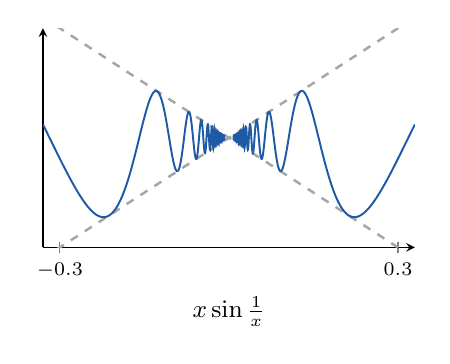
\begin{tikzpicture}
\begin{axis}[nfig, xmin=-0.33, xmax=0.33, ymin=-0.3, ymax=0.3,
  xtick={-0.3,0.3}, ytick=\empty, xlabel={$x\sin\frac1x$}]
  \addplot[black!35, dashed, domain=-0.33:0.33] {x};
  \addplot[black!35, dashed, domain=-0.33:0.33] {-x};
  \addplot[figB, domain=0.008:0.33, samples=900, line width=0.7pt] {x*sin(deg(1/x))};
  \addplot[figB, domain=-0.33:-0.008, samples=900, line width=0.7pt] {x*sin(deg(1/x))};
\end{axis}
\end{tikzpicture}%
\hfill
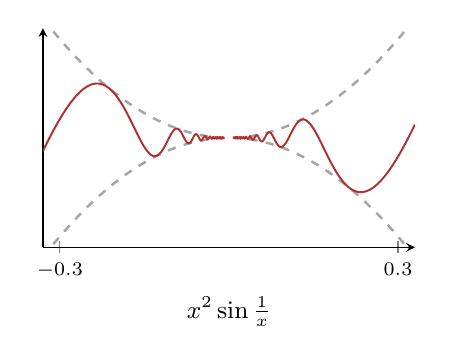
\begin{tikzpicture}
\begin{axis}[nfig, xmin=-0.33, xmax=0.33, ymin=-0.1, ymax=0.1,
  xtick={-0.3,0.3}, ytick=\empty, xlabel={$x^2\sin\frac1x$}]
  \addplot[black!35, dashed, domain=-0.33:0.33, samples=60] {x^2};
  \addplot[black!35, dashed, domain=-0.33:0.33, samples=60] {-x^2};
  \addplot[figR, domain=0.008:0.33, samples=900, line width=0.7pt] {x^2*sin(deg(1/x))};
  \addplot[figR, domain=-0.33:-0.008, samples=900, line width=0.7pt] {x^2*sin(deg(1/x))};
\end{axis}
\end{tikzpicture}\figcap{The oscillation ladder with its envelopes (dashed): $x \sin\tfrac1x$ hugs $\pm x$ --- continuous at $0$, not differentiable; $x^2 \sin\tfrac1x$ hugs $\pm x^2$ --- differentiable, but $f'$ oscillates without limit. Each extra power of damping flattens the envelope by one order at the origin.}
\end{center}


Computations with piecewise functions --- the corner examples above --- all follow one pattern. It deserves a statement:

\begin{propbox}[Differentiability of a Piecewise Function (HW)]
Let $f, g$ be differentiable on an open interval $I$, let $a \in I$, and define
\[
h(x) = \begin{cases} f(x), & x < a, \\ g(x), & x \geq a. \end{cases}
\]
Then $h$ is differentiable at $a$ if and only if \emph{both}
\[
f(a) = g(a) \qquad \text{and} \qquad f'(a) = g'(a)
\]
hold --- the two branches must agree in \emph{value} and in \emph{slope} --- and in that case $h'(a)$ is the common value $f'(a) = g'(a)$.
\end{propbox}

\begin{proof}
Note $h(a) = g(a)$ by definition.

($\Rightarrow$) If $h$ is differentiable at $a$, it is continuous there; the left limit is $\lim_{x \to a^-} f(x) = f(a)$ ($f$ continuous, being differentiable), and it must equal $h(a) = g(a)$: value match. Then the two one-sided difference quotients of $h$,
\[
\lim_{x \to a^-} \frac{f(x) - f(a)}{x - a} = f'(a), \qquad
\lim_{x \to a^+} \frac{g(x) - g(a)}{x - a} = g'(a)
\]
(using $h(a) = f(a) = g(a)$ on the left), both exist and must equal the two-sided limit $h'(a)$: slope match.

($\Leftarrow$) With $f(a) = g(a)$, the same two computations show the one-sided limits of $\tfrac{h(x)-h(a)}{x-a}$ are $f'(a)$ and $g'(a)$; if these agree, the two-sided limit exists and $h'(a) = f'(a) = g'(a)$.
\end{proof}

\begin{rembox}
Read backwards, this organizes every corner in this section: $|x|$ glues $-x$ and $x$ at $0$ with matching values ($0 = 0$) but slopes $-1 \neq 1$ --- corner; more generally, $|u|$ has a corner at every point where $u$ crosses $0$ with $u' \neq 0$ (slopes $\pm u'$), while at a zero of $u$ with $u' = 0$ the glue is smooth. Read forwards, it is the design rule for splines: to join two formulas differentiably, match value and slope at the seam.
\end{rembox}

% ============================================================================
% SECTION 29: THE MEAN VALUE THEOREM
% ============================================================================

\section{The Mean Value Theorem}

We come to an important section --- the first of the three main results of this chapter.

\subsection{Interior Extrema and Rolle's Theorem}

\begin{thmbox}[Interior Extremum Theorem]
Suppose $f: (a,b) \to \mathbb{R}$ has a maximum or minimum value at $x_0$. If $f$ is differentiable at $x_0$, then
\[
f'(x_0) = 0.
\]
\end{thmbox}

Note the interval is \emph{open}: it has no boundary points, so $x_0$ is automatically an interior point. This is well known from calculus: a maximum or minimum point inside an interval is a \textbf{critical point} ($f'(x_0) = 0$).

\begin{proof}
By definition! Assume $f$ has a maximum at $x_0$ (the minimum case is symmetric). The limit
\[
f'(x_0) = \lim_{x\to x_0} \frac{f(x) - f(x_0)}{x - x_0}
\]
exists, so both one-sided limits exist and equal it (\S 20). Now read the signs: for $x > x_0$, the numerator $f(x) - f(x_0) \leq 0$ (maximum!) while $x - x_0 > 0$, so the quotient is $\leq 0$, and limits preserve $\leq$:
\[
\lim_{x \to x_0^+} \frac{f(x) - f(x_0)}{x - x_0} \leq 0.
\]
For $x < x_0$ the quotient is $\geq 0$, so the left-hand limit is $\geq 0$. Both equal $f'(x_0)$, forcing $f'(x_0) = 0$.
\end{proof}

\begin{thmbox}[Rolle's Theorem]
Let $f: [a,b] \to \mathbb{R}$ be continuous, and differentiable at every point of $(a,b)$ (briefly: differentiable on $(a,b)$). If $f(a) = f(b)$, then there exists $x_0 \in (a,b)$ with
\[
f'(x_0) = 0.
\]
\end{thmbox}

\begin{proof}
By the Extreme Value Theorem (\S 18), $f$ attains a maximum at some $x_1 \in [a,b]$ and a minimum at some $x_2 \in [a,b]$. Since $x_1, x_2$ could be endpoints, we cannot apply the previous theorem yet --- two cases.

\emph{Case $f(x_1) = f(x_2)$:} the maximum equals the minimum, so every value of $f$ is squeezed between equal bounds --- $f$ is constant. Then $f'(x_0) = 0$ for \emph{every} $x_0 \in (a,b)$.

\emph{Case $f(x_1) > f(x_2)$:} since $f(a) = f(b)$, the two extreme values cannot both equal the common endpoint value; say $f(x_1) \neq f(a) = f(b)$ (otherwise argue with $x_2$). Then $x_1 \neq a, b$, so $x_1 \in (a,b)$: an interior maximum. By the previous theorem, $f'(x_1) = 0$.
\end{proof}

\subsection{The Mean Value Theorem and Its Corollaries}

\begin{thmbox}[Mean Value Theorem]
Let $f: [a,b] \to \mathbb{R}$ be continuous and differentiable on $(a,b)$. Then there exists $x_0 \in (a,b)$ such that
\[
f'(x_0) = \frac{f(b) - f(a)}{b - a}, \qquad \text{i.e.} \qquad f(b) - f(a) = f'(x_0)(b-a).
\]
\end{thmbox}

Two interpretations: (1) \emph{slopes} --- some tangent line is parallel to the chord through the endpoints; (2) \emph{the average rate of change equals the rate of change at some one point}.

\begin{proof}
Reduce to Rolle by subtracting the chord. Let $L$ be the linear function agreeing with $f$ at the endpoints:
\[
L(x) = f(a) + \frac{f(b) - f(a)}{b-a}\,(x - a), \qquad L(a) = f(a),\ L(b) = f(b), \qquad L'(x) = \frac{f(b)-f(a)}{b-a}.
\]
Set $g(x) = f(x) - L(x)$: continuous on $[a,b]$, differentiable on $(a,b)$, with $g(a) = g(b) = 0$. Rolle's theorem gives $x_0 \in (a,b)$ with $g'(x_0) = 0$, i.e.
\[
f'(x_0) - \frac{f(b)-f(a)}{b-a} = 0. \qedhere
\]
\end{proof}

\begin{center}
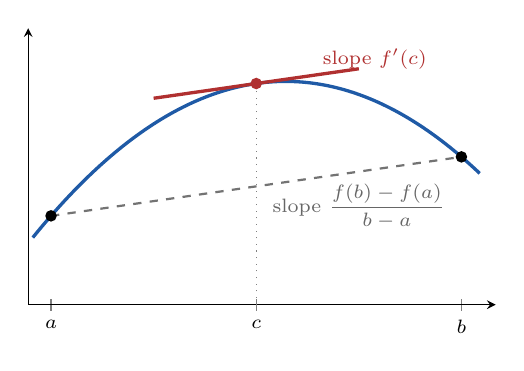
\begin{tikzpicture}
\begin{axis}[nfig, width=0.62\textwidth, height=0.42\textwidth,
  xmin=0, xmax=2.05, ymin=0, ymax=1.35,
  xtick={0.1,1.0,1.9}, xticklabels={$a$,$c$,$b$}, ytick=\empty, xlabel={}]
  \addplot[black!55, dashed, thick] coordinates {(0.1,0.4338) (1.9,0.7218)};
  \addplot[figB, very thick, domain=0.02:1.98, samples=120] {0.3+1.4*x-0.62*x^2};
  \addplot[figR, very thick, domain=0.55:1.45] {1.08+0.16*(x-1)};
  \addplot[only marks, mark=*, mark size=1.6pt, black] coordinates {(0.1,0.4338) (1.9,0.7218)};
  \addplot[only marks, mark=*, mark size=1.6pt, figR] coordinates {(1.0,1.08)};
  \draw[black!50, dotted] (axis cs:1.0,0) -- (axis cs:1.0,1.08);
  \node[font=\scriptsize, figR] at (axis cs:1.52,1.20) {slope $f'(c)$};
  \node[font=\scriptsize, black!60] at (axis cs:1.45,0.48) {slope $\dfrac{f(b)-f(a)}{b-a}$};
\end{axis}
\end{tikzpicture}\figcap{The Mean Value Theorem: somewhere in $(a,b)$ the tangent (red) is parallel to the secant (dashed). Rolle is the horizontal special case; the proof above is literally this picture --- subtract the secant, and the extremum of what remains is $c$.}
\end{center}


\begin{corbox}[Vanishing Derivative Means Constant]
If $f: (a,b) \to \mathbb{R}$ is differentiable and $f'(x) = 0$ for all $x \in (a,b)$, then $f$ is constant.
\end{corbox}

\begin{proof}
Seems well known --- but how to prove it? (The book has a proof by contradiction; here is a direct one.) For any two points $x_1 < x_2$ in $(a,b)$, the MVT on $[x_1, x_2]$ gives $x_0 \in (x_1, x_2)$ with
\[
f(x_2) - f(x_1) = f'(x_0)(x_2 - x_1) = 0 \cdot (x_2 - x_1) = 0.
\]
So $f$ takes the same value at any two points. Done.
\end{proof}

\begin{corbox}[Equal Derivatives Differ by a Constant]
If $f, g: (a,b) \to \mathbb{R}$ are differentiable with $f'(x) = g'(x)$ for all $x$, then $f = g + c$ for some constant $c$.
\end{corbox}

\begin{proof}
Apply the previous corollary to $f - g$, whose derivative vanishes identically.
\end{proof}

\begin{propbox}[Vanishing k-th Derivative Means Polynomial (HW)]
Let $k \geq 1$ and let $f$ be $k$ times differentiable on an open interval $I$ with $f^{(k)} \equiv 0$ on $I$. Then $f$ is a polynomial of degree less than $k$; conversely, every such polynomial has vanishing $k$-th derivative.
\end{propbox}

\begin{proof}
The converse is a direct computation. Forward, by induction on $k$. The case $k = 1$ is the constant corollary. Suppose the claim holds for $k$, and let $f^{(k+1)} \equiv 0$. Then $(f')^{(k)} = f^{(k+1)} \equiv 0$, so by the induction hypothesis $f'$ is a polynomial of degree less than $k$, say $f'(x) = \sum_{j=0}^{k-1} c_j x^j$. The polynomial $g(x) = \sum_{j=0}^{k-1} \tfrac{c_j}{j+1}\, x^{j+1}$ satisfies $g' = f'$ on $I$, so by the previous corollary $f = g + c$: a polynomial of degree at most $k$, i.e.\ less than $k + 1$.
\end{proof}

\begin{rembox}
This identifies the \emph{kernel} of the $k$-th derivative operator: exactly the polynomials of degree $< k$ --- a $k$-dimensional space, matching the $k$ constants of integration. It is also the uniqueness half of Taylor's theory (\S 31): once the remainder is shown to vanish, this proposition is what forces $f$ to \emph{be} its Taylor polynomial.
\end{rembox}

\begin{corbox}[Sign of the Derivative and Monotonicity]
Let $f: (a,b) \to \mathbb{R}$ be differentiable. If $f'(x) \geq 0$ for all $x$, then $f$ is increasing; if $f'(x) \leq 0$ for all $x$, then $f$ is decreasing.
\end{corbox}

\begin{proof}
For $x_1 < x_2$ in $(a,b)$, the MVT gives $x_0$ with $f(x_2) - f(x_1) = f'(x_0)(x_2 - x_1)$, whose sign is the sign of $f'(x_0)$. (With strict inequalities $f' > 0$ throughout, the same display gives \emph{strictly} increasing.)
\end{proof}

\subsection{Applications}

\begin{exbox}[Squared-distance contraction]
Suppose $f: \mathbb{R} \to \mathbb{R}$ satisfies $|f(x) - f(y)| \leq |x - y|^2$ for all $x, y$. Then $f$ is constant.

\emph{Proof.} For $x \neq y$,
\[
\left| \frac{f(x) - f(y)}{x - y} \right| \leq |x - y| \longrightarrow 0 \quad \text{as } x \to y,
\]
so $f$ is differentiable at every $y$ with $f'(y) = 0$ (squeeze). By the corollary, $f$ is constant. \hfill $\blacksquare$
\end{exbox}

\begin{exbox}[The tangent line inequality for the exponential]
Prove: $e^x \geq ex$ for all $x \in \mathbb{R}$ (with equality at $x = 1$: the graph of $e^x$ lies above its tangent line at $(1, e)$).

Let $f(x) = ex - e^x$; we want $f(x) \leq 0$. Note $f(1) = e - e = 0$. Check the derivative:
\[
f'(x) = e - e^x: \qquad f'(x) > 0 \text{ for } x < 1, \qquad f'(x) < 0 \text{ for } x > 1.
\]
So $f$ is increasing on $(-\infty, 1)$ and decreasing on $(1, \infty)$ (previous corollary): $x = 1$ is a global maximum with value $0$. Hence $f(x) \leq 0$ everywhere. \hfill $\blacksquare$
\end{exbox}

\begin{exbox}[Sine below its argument]
Show $\sin x \leq x$ for all $x \geq 0$. Let $f(x) = x - \sin x$; then $f(0) = 0$ and
\[
f'(x) = 1 - \cos x \geq 0,
\]
so $f$ is increasing on $[0,\infty)$, giving $f(x) \geq f(0) = 0$, i.e.\ $\sin x \leq x$ for $x \geq 0$. Similarly (or by oddness: replace $x$ by $-x$), $\sin x \geq x$ for all $x \leq 0$. \hfill $\blacksquare$
\end{exbox}

The three examples above are one-sided instances of a two-sided principle:

\begin{propbox}[Mean Value Inequality (HW)]
Suppose $f$ is continuous on $[a,b]$, differentiable on $(a,b)$, and $m \leq f'(x) \leq M$ for all $x \in (a,b)$. Then
\[
m\,(b-a) \;\leq\; f(b) - f(a) \;\leq\; M\,(b-a).
\]
Bounds on the derivative become bounds on every increment.
\end{propbox}

\begin{proof}
The MVT gives $c \in (a,b)$ with $f(b) - f(a) = f'(c)(b-a)$; squeeze $f'(c)$ between $m$ and $M$ and multiply by $b - a > 0$.
\end{proof}

For instance: if $f$ is differentiable on $\mathbb{R}$ with $1 \leq f' \leq 2$ everywhere and $f(0) = 0$, then applying the proposition on $[0, x]$ gives $x \leq f(x) \leq 2x$ for every $x \geq 0$ --- the graph is trapped between two lines through the origin.

\begin{exbox}[An integrating factor for Rolle (HW)]
Let $f, g$ be differentiable on an open interval $I$, and let $a < b$ in $I$ with $f(a) = f(b) = 0$. Show that
\[
f'(x) + f(x)\,g'(x) = 0 \qquad \text{for some } x \in (a,b).
\]
The expression is not the derivative of anything obvious --- so \emph{make} it one. Multiply by the always-positive factor $e^{g}$: the function $h = f\, e^{g}$ is differentiable on $I$ with
\[
h'(x) = e^{g(x)} \left[ f'(x) + f(x)\, g'(x) \right],
\]
and $h(a) = h(b) = 0$ since $f$ vanishes there. Rolle's theorem hands us $x_0 \in (a,b)$ with $h'(x_0) = 0$; dividing by $e^{g(x_0)} \neq 0$ leaves $f'(x_0) + f(x_0)g'(x_0) = 0$. \hfill $\blacksquare$
\end{exbox}

\begin{rembox}
The multiplier $e^{g}$ is the \emph{integrating factor} of differential equations in embryo: the equation $y' + y\,g' = 0$ is exactly $(y e^{g})' = 0$, i.e.\ $y = C e^{-g}$. The general pattern is worth remembering: to prove some expression $E(x)$ vanishes somewhere, hunt for an auxiliary $h$ with equal endpoint values whose derivative is (positive function) $\times\, E$ --- then Rolle does the rest. The MVT's own proof (tilting by a linear function) and the Generalized MVT of \S 30 are the same trick with different auxiliaries.
\end{rembox}

\subsection{The Intermediate Value Theorem for Derivatives}

Recall the Intermediate Value Theorem for continuous functions (\S 18). Derivatives satisfy their own version --- remarkably, \emph{without} assuming $f'$ continuous:

\begin{thmbox}[Darboux's Theorem]
Let $f: [a,b] \to \mathbb{R}$ be continuous and differentiable on $(a,b)$. Let $a < x_1 < x_2 < b$ and let $c$ lie between $f'(x_1)$ and $f'(x_2)$. Then there exists $x_0 \in (x_1, x_2)$ with
\[
f'(x_0) = c.
\]
\end{thmbox}

\begin{rembox}
The point of the theorem: $f'$ may fail to be continuous (standard example: $f(x) = x^2 \sin\tfrac1x$, $f(0)=0$, whose derivative exists everywhere but is discontinuous at $0$), so we \emph{cannot} simply apply the IVT of \S 18 to $f'$. Yet derivatives still take intermediate values.
\end{rembox}

\begin{proof}
Assume $f'(x_1) < c < f'(x_2)$ (for the reversed case, consider the maximum instead of the minimum below, or apply the result to $-f$). Following the general pattern --- introduce a new function and find a critical point --- let
\[
g(x) = f(x) - cx, \qquad g'(x_1) = f'(x_1) - c < 0, \quad g'(x_2) = f'(x_2) - c > 0.
\]
$g$ is continuous on $[x_1, x_2]$, so it attains a minimum at some $x_0 \in [x_1, x_2]$ (EVT).

\emph{Claim: $x_0 \neq x_1, x_2$.} Since $g'(x_1) < 0$, the difference quotient $\tfrac{g(x) - g(x_1)}{x - x_1}$ is negative for $x$ slightly to the right of $x_1$ (its limit is negative); for such $x$, $x - x_1 > 0$ forces $g(x) < g(x_1)$ --- nearby points in $(x_1, x_2)$ have \emph{smaller} values, so $x_1$ is not the minimum. Symmetrically, $g'(x_2) > 0$ means points slightly to the \emph{left} of $x_2$ have smaller values, so $x_2$ is not the minimum either.

Hence $x_0 \in (x_1, x_2)$ is an interior minimum, and the Interior Extremum Theorem gives $g'(x_0) = 0$, i.e.\ $f'(x_0) = c$.
\end{proof}

\begin{exbox}[Prescribed derivative values]
Let $f: \mathbb{R} \to \mathbb{R}$ be differentiable with $f(0) = 0$, $f(1) = 1$, $f(2) = 1$.

\textbf{(a)} Some $x_0 \in (0,2)$ has $f'(x_0) = \tfrac12$: by the MVT on $[0,2]$,
\[
f'(x_0) = \frac{f(2) - f(0)}{2 - 0} = \frac12.
\]

\textbf{(b)} Some $x_0 \in (0,2)$ has $f'(x_0) = \tfrac17$: the MVT on $[0,1]$ gives $x_1 \in (0,1)$ with $f'(x_1) = \tfrac{1-0}{1-0} = 1$, and on $[1,2]$ gives $x_2 \in (1,2)$ with $f'(x_2) = \tfrac{1-1}{2-1} = 0$. Since $0 < \tfrac17 < 1$, Darboux's theorem applied between $x_1 < x_2$ produces $x_0 \in (x_1, x_2) \subset (0,2)$ with $f'(x_0) = \tfrac17$. (This second method also reproves (a).) \hfill $\blacksquare$
\end{exbox}

\subsection{The Derivative of the Inverse Function}

Suppose $y = f(x)$ has an inverse $x = f^{-1}(y)$. \emph{If we already knew} $f^{-1}$ were differentiable at $y_0 = f(x_0)$, the chain rule applied to $f^{-1}(f(x)) = x$ would give
\[
(f^{-1})'(y_0)\, f'(x_0) = 1, \qquad \text{i.e.} \qquad (f^{-1})'(y_0) = \frac{1}{f'(x_0)}.
\]
This computation finds the \emph{formula} but presupposes the differentiability of $f^{-1}$ --- which is exactly what the theorem must supply:

\begin{thmbox}[Inverse Function Theorem]
Let $I$ be an open interval and $f: I \to J = f(I)$ a continuous one-to-one map onto an open interval $J$, so that $f^{-1}: J \to I$ exists. If $f$ is differentiable at $x_0 \in I$ with $f'(x_0) \neq 0$, then $f^{-1}$ is differentiable at $y_0 = f(x_0)$, and
\[
(f^{-1})'(y_0) = \frac{1}{f'(x_0)}.
\]
\end{thmbox}

\begin{proof}
Since $f$ is injective, $f(x) \neq f(x_0)$ for all $x \neq x_0$, so the reciprocal difference quotient is defined, and since $f'(x_0) \neq 0$, the reciprocal limit theorem gives
\[
\lim_{x \to x_0} \frac{x - x_0}{f(x) - f(x_0)} = \frac{1}{f'(x_0)}.
\]
Now translate into the $y$-variable. Write $g = f^{-1}$; a continuous injective function on an interval is strictly monotone (if not, three points would violate the IVT), so by the Continuous Inverse Theorem of \S 18 (extended to open intervals), $g$ is continuous. Let $y_n \to y_0$ in $J$ with $y_n \neq y_0$, and set $x_n = g(y_n)$. By continuity of $g$, $x_n \to x_0$, and by injectivity $x_n \neq x_0$. Then, by the sequential characterization of the limit above,
\[
\frac{g(y_n) - g(y_0)}{y_n - y_0} = \frac{x_n - x_0}{f(x_n) - f(x_0)} \longrightarrow \frac{1}{f'(x_0)}.
\]
Since the sequence $(y_n)$ was arbitrary, $g'(y_0)$ exists and equals $\tfrac{1}{f'(x_0)}$.
\end{proof}

\begin{rembox}
The assumption $f'(x_0) \neq 0$ is important: think of $f(x) = x^3$ at $x_0 = 0$ --- the inverse $y \mapsto y^{1/3}$ exists but is not differentiable at $0$ (vertical tangent). Behind the theorem: $f'(x_0) \neq 0$ makes $f$ strictly monotone near $x_0$, so an inverse exists locally --- a principle that generalizes far beyond calculus (the \emph{inverse function theorem} of advanced analysis).
\end{rembox}

\begin{exbox}[Arcsine]
$f(x) = \sin x$ restricted to $\left[-\tfrac\pi2, \tfrac\pi2\right]$ (needed for $\arcsin$ to be well defined --- draw the graph of $\sin$), with inverse $f^{-1}(y) = \arcsin y$:
\[
(\arcsin y)' = \frac{1}{\cos x} = \frac{1}{\sqrt{1 - \sin^2 x}} = \frac{1}{\sqrt{1 - y^2}},
\]
where $\cos x = +\sqrt{1 - \sin^2 x}$ is legitimate because $\cos x \geq 0$ on $\left[-\tfrac\pi2, \tfrac\pi2\right]$. \hfill $\blacksquare$
\end{exbox}

\begin{exbox}[Arctangent (HW)]
The same machine, one branch simpler. On $I = \left( -\tfrac\pi2, \tfrac\pi2 \right)$, $f(x) = \tan x$ has (quotient rule, Pythagoras)
\[
f'(x) = \frac{\cos^2 x + \sin^2 x}{\cos^2 x} = \frac{1}{\cos^2 x} > 0,
\]
so $f$ is strictly increasing with never-vanishing derivative, mapping $I$ onto $\mathbb{R}$. The Inverse Function Theorem applies at every point --- no endpoint or sign caveats this time, unlike arcsine --- and for $y_0 = \tan x_0$,
\[
\arctan'(y_0) = \frac{1}{f'(x_0)} = \cos^2 x_0 = \frac{1}{1 + \tan^2 x_0} = \frac{1}{1 + y_0^2},
\]
converting to the $y$-variable by dividing $\sin^2 + \cos^2 = 1$ through by $\cos^2$. So
\[
\arctan'(x) = \frac{1}{1+x^2} \qquad \text{on all of } \mathbb{R}
\]
--- the derivative on which the arctangent series of \S 26 stands. \hfill $\blacksquare$
\end{exbox}

% ============================================================================
% SECTION 30: L'HOSPITAL'S RULE
% ============================================================================

\section{L'Hospital's Rule}

Now the most interesting section --- with a good story about learning: paying for knowledge and fame (L'Hospital famously bought the result from Johann Bernoulli). We often meet limits of the type
\[
\lim_{x\to s} \frac{f(x)}{g(x)}, \qquad \text{where } f(x) \to 0,\ g(x) \to 0, \quad \text{or} \quad f(x) \to \infty,\ g(x) \to \infty
\]
--- problematic, since no value can be given to $\tfrac00$ or $\tfrac\infty\infty$ (\S 5). Examples: $\lim_{x\to0}\tfrac{\sin x}{x}$ (type $\tfrac00$), $\lim_{x\to+\infty} \tfrac{x}{e^x}$ (type $\tfrac\infty\infty$).

\begin{thmbox}[L'Hospital's Rule]
Suppose $\lim_{x\to s} f(x) = 0 = \lim_{x\to s} g(x)$, \emph{or} $\lim_{x\to s} |g(x)| = \infty$; suppose $f, g$ are differentiable (with $g'(x) \neq 0$) near $s$. If
\[
\lim_{x\to s} \frac{f'(x)}{g'(x)} = L,
\]
then
\[
\lim_{x\to s} \frac{f(x)}{g(x)} = L.
\]
Here $s$ can be a finite number or $\pm\infty$, the limits can be one-sided ($x \to s^+$ or $x \to s^-$), and $L$ may be finite or $\pm\infty$.
\end{thmbox}

The idea: differentiating can \emph{simplify} $f$ and $g$, letting us escape the indeterminate forms. We use the rule first, then prove it.

\subsection{Using the Rule}

\begin{exbox}[Four computations]
\textbf{(1)} $\displaystyle\lim_{x\to0} \frac{\sin x}{x} = \lim_{x\to0} \frac{\cos x}{1} = \frac11 = 1$ --- after differentiating, the denominator is $1 \neq 0$ and $\cos$ is continuous: the difficulty has been avoided.

\textbf{(2)} $\displaystyle\lim_{x\to+\infty} \frac{x}{e^x} = \lim_{x\to+\infty} \frac{1}{e^x} = 0$ (type $\tfrac\infty\infty$; this finally makes rigorous the growth comparison borrowed in \S 9).

\textbf{(3)} $\displaystyle\lim_{x\to0} \frac{1 - \cos x}{x^2} = \lim_{x\to0} \frac{\sin x}{2x} = \lim_{x\to0} \frac{\cos x}{2} = \frac12$ --- two applications in a row, each hypothesis re-checked (the intermediate quotient is again $\tfrac00$).

\textbf{(4)} $\displaystyle\lim_{x\to0^+} x \log x$ --- type $0 \cdot \infty$; convert to a standard form:
\[
\lim_{x\to0^+} x\log x = \lim_{x\to0^+} \frac{\log x}{\tfrac1x} = \lim_{x\to0^+} \frac{\tfrac1x}{-\tfrac1{x^2}} = \lim_{x\to0^+} (-x) = 0.
\]
\emph{But beware}: rewriting instead as $\tfrac{x}{1/\log x}$ and differentiating makes the expression \emph{more} complicated --- the rule does not tell you \emph{which} rewriting to choose. This is one thing to remember. \hfill $\blacksquare$
\end{exbox}

\begin{exbox}[The form zero to the zero]
Compute $\lim_{x\to0^+} x^x$ --- type $0^0$: since $a^0 = 1$ for $a > 0$ but $0^a = 0$, we don't know right away. The trick: exponentials convert products into the standard forms,
\[
x^x = e^{\log x^x} = e^{x \log x},
\]
reducing to example (4): $x\log x \to 0$, so by continuity of the exponential,
\[
\lim_{x\to0^+} x^x = e^0 = 1. \tag*{$\blacksquare$}
\]
\end{exbox}

\subsection{Proving the Rule: the Generalized Mean Value Theorem}

We prove a special case: $f(x) \to 0$, $g(x) \to 0$ as $x \to a^-$, with finite $a$ and finite $L$. (The $\tfrac\infty\infty$ case and $s = \pm\infty$ are similar in spirit; see the book.) The idea: for $x < x_1 < a$ with both close to $a$,
\[
\frac{f(x)}{g(x)} \approx \frac{f(x) - f(x_1)}{g(x) - g(x_1)},
\]
since $f(x_1), g(x_1)$ are very small --- and the right side, by the following theorem, is an honest derivative quotient.

\begin{thmbox}[Generalized Mean Value Theorem]
Let $f, g: [a,b] \to \mathbb{R}$ be continuous and differentiable on $(a,b)$. Then there exists $x_0 \in (a,b)$ such that
\[
\bigl(f(b) - f(a)\bigr)\, g'(x_0) = \bigl(g(b) - g(a)\bigr)\, f'(x_0).
\]
In particular, when $g(b) - g(a) \neq 0$ (and $g'(x_0) \neq 0$),
\[
\frac{f(b) - f(a)}{g(b) - g(a)} = \frac{f'(x_0)}{g'(x_0)}.
\]
The symmetric formulation avoids any difficulty with $g(b) - g(a) = 0$; taking $g(x) = x$ recovers the ordinary MVT.
\end{thmbox}

\begin{proof}
Following the pattern, define a new function whose critical point we seek:
\[
F(x) = \bigl(f(b) - f(a)\bigr) g(x) - \bigl(g(b) - g(a)\bigr) f(x).
\]
Compute the endpoint values --- the cross terms survive:
\[
F(a) = f(b)g(a) - g(b)f(a), \qquad F(b) = f(b)g(a) - g(b)f(a) = F(a).
\]
By Rolle's theorem, there is $x_0 \in (a,b)$ with $F'(x_0) = 0$, which is exactly the claimed identity.
\end{proof}

\begin{proof}[Proof of L'Hospital's Rule (special case)]
Assume $f, g \to 0$ as $x \to a^-$, $g' \neq 0$ on some $(a - \delta_0, a)$, and $\tfrac{f'}{g'} \to L$ finite. First, two housekeeping points on $(a-\delta_0, a)$: for $x < x_1$ there, $g(x_1) \neq g(x)$ (otherwise Rolle would give a zero of $g'$ in between); and $g(x) \neq 0$ for $x$ close to $a$ (if $g$ vanished at points arbitrarily close to $a$, Rolle between two such zeros would again contradict $g' \neq 0$).

Let $\varepsilon > 0$. Choose $\delta \leq \delta_0$ such that
\[
\left| \frac{f'(t)}{g'(t)} - L \right| < \varepsilon \qquad \text{for all } t \in (a - \delta,\, a).
\]
Fix any $x \in (a-\delta, a)$, and let $x_1 \in (x, a)$. By the Generalized MVT on $[x, x_1]$, there is $x_2 \in (x, x_1) \subset (a-\delta, a)$ with
\[
\frac{f(x) - f(x_1)}{g(x) - g(x_1)} = \frac{f'(x_2)}{g'(x_2)}, \qquad \text{hence} \qquad \left| \frac{f(x) - f(x_1)}{g(x) - g(x_1)} - L \right| < \varepsilon.
\]
Now let $x_1 \to a^-$ with $x$ held fixed: $f(x_1) \to 0$ and $g(x_1) \to 0$, so the quotient tends to $\tfrac{f(x)}{g(x)}$, and limits preserve the closed bound:
\[
\left| \frac{f(x)}{g(x)} - L \right| \leq \varepsilon \qquad \text{for every } x \in (a - \delta, a).
\]
Since $\varepsilon$ was arbitrary, $\lim_{x\to a^-} \tfrac{f(x)}{g(x)} = L$. (This $\varepsilon$-argument is the rigorous form of the approximation idea sketched above.)
\end{proof}

\subsection{More Indeterminate Forms}

\begin{exbox}[One to the infinity]
Compute $\displaystyle\lim_{x\to\infty} \left( 1 - \frac2x \right)^x$ --- type $1^\infty$, undetermined. Transform through the exponential:
\[
\left(1 - \frac2x\right)^x = e^{x \log\left(1 - \frac2x\right)},
\]
and the exponent, of type $\infty \cdot 0$, transforms again:
\[
x \log\left(1 - \frac2x\right) = \frac{\log\left(1 - \frac2x\right)}{\frac1x}
\ \xrightarrow{\text{L'H}}\
\frac{\left(1 - \frac2x\right)^{-1} \cdot \frac{2}{x^2}}{-\frac{1}{x^2}} = -\frac{2}{1 - \frac2x} \longrightarrow -2.
\]
By continuity of the exponential, the answer is $e^{-2}$. \hfill $\blacksquare$
\end{exbox}

\begin{exbox}[Infinity minus infinity]
Compute $\displaystyle\lim_{x\to0} \left( \frac{1}{e^x - 1} - \frac{1}{x} \right)$ --- type $\infty - \infty$. Combine over a common denominator to reach $\tfrac00$:
\[
\frac{1}{e^x-1} - \frac1x = \frac{x - e^x + 1}{x(e^x - 1)}
\ \xrightarrow{\text{L'H}}\
\frac{1 - e^x}{e^x - 1 + x e^x}
\ \xrightarrow{\text{L'H}}\
\frac{-e^x}{2e^x + x e^x} \longrightarrow \frac{-1}{2}.
\]
(Each application re-checked: both intermediate quotients are $\tfrac00$ at $x = 0$.) So the limit is $-\tfrac12$. \hfill $\blacksquare$
\end{exbox}

\subsection{Abstract Applications}

Sometimes we deal with abstract functions rather than explicit formulas.

\begin{exbox}[Recovering the limit of f from a combination]
Let $f: (c, \infty) \to \mathbb{R}$ be differentiable and suppose $\lim_{x\to\infty} \bigl(f(x) + f'(x)\bigr) = L$. Prove $\lim_{x\to\infty} f(x) = L$.

\emph{Proof.} Rewrite with an exponential weight:
\[
f(x) = \frac{f(x)e^x}{e^x}.
\]
The denominator $e^x \to \infty$, so L'Hospital's rule applies (note: the $|g| \to \infty$ case requires \emph{nothing} of the numerator!). The quotient of derivatives is
\[
\frac{\bigl(f(x)e^x\bigr)'}{(e^x)'} = \frac{\bigl(f'(x) + f(x)\bigr)e^x}{e^x} = f'(x) + f(x) \longrightarrow L,
\]
hence $f(x) \to L$. Similarly, if $\lim_{x\to\infty}\bigl(2f(x) + f'(x)\bigr) = L$, write $f = \tfrac{f e^{2x}}{e^{2x}}$; the derivative quotient is $\tfrac{(f' + 2f)e^{2x}}{2e^{2x}} = \tfrac{f' + 2f}{2} \to \tfrac L2$, so $\lim f(x) = \tfrac L2$. \hfill $\blacksquare$
\end{exbox}

\begin{exbox}[Another one-to-the-infinity]
$\displaystyle\lim_{x\to\infty}\left(1 - \frac1x\right)^x = e^{-1}$, by the same method as $\left(1-\tfrac2x\right)^x$ in the previous subsection (the exponent $x\log(1-\tfrac1x) \to -1$).
\end{exbox}

% ============================================================================
% SECTION 31: TAYLOR'S THEOREM
% ============================================================================

\section{Taylor's Theorem}

The third main result of the chapter: how to approximate general functions by polynomials --- and, in the limit, represent a function by a power series.

\subsection{The Taylor Series}

Suppose first that $f(x) = \sum_{n=0}^\infty a_n x^n$ converges for $|x| < R$. What are the coefficients, in terms of $f$? By \S 26, term-by-term differentiation is valid and preserves the radius, so it can be \emph{iterated}:
\[
f(0) = a_0; \qquad f'(x) = \sum_{n\geq1} n a_n x^{n-1}, \quad f'(0) = a_1; \qquad f''(x) = \sum_{n \geq 2} n(n-1) a_n x^{n-2}, \quad f''(0) = 2! \, a_2;
\]
and in general, differentiating $n$ times and evaluating at $0$ kills all terms except the constant one:
\[
f^{(n)}(0) = n!\, a_n, \qquad \text{i.e.} \qquad a_n = \frac{f^{(n)}(0)}{n!}.
\]
So a convergent power series is forced to be $\sum \tfrac{f^{(n)}(0)}{n!} x^n$. This motivates:

\begin{defbox}[Taylor Series]
If $f: (-\varepsilon, \varepsilon) \to \mathbb{R}$ has derivatives of all orders at $0$, the series
\[
\sum_{n=0}^\infty \frac{f^{(n)}(0)}{n!}\, x^n
\]
is called the \textbf{Taylor series of $f$ at $0$}. (The $\varepsilon$ signals, as in $\varepsilon$-$\delta$ arguments, that only a small neighborhood matters --- how big the domain is, we don't care.) More generally, for $f: (a,b) \to \mathbb{R}$ with derivatives of all orders and $x_0 \in (a,b)$, the \textbf{Taylor series at $x_0$} is $\sum_n \tfrac{f^{(n)}(x_0)}{n!} (x - x_0)^n$. We concentrate on $x_0 = 0$.
\end{defbox}

\textbf{Question: is $f(x) = \sum_n \tfrac{f^{(n)}(0)}{n!}x^n$ for every $f$ with all derivatives?} No --- two distinct problems:
\begin{enumerate}[label=(\arabic*)]
    \item the Taylor series may not converge for any $x \neq 0$ (radius $R = 0$);
    \item even if $R > 0$, the series may converge to something \emph{other than} $f(x)$.
\end{enumerate}

\subsection{The Remainder and Taylor's Theorem}

Convergence of the series to $f$ is governed by the partial sums $s_n(x) = \sum_{k=0}^{n} \tfrac{f^{(k)}(0)}{k!}x^k$. Define the \textbf{remainder}
\[
R_n(x) = f(x) - s_{n-1}(x) = f(x) - \sum_{k=0}^{n-1} \frac{f^{(k)}(0)}{k!} x^k.
\]

\begin{propbox}[Convergence via the Remainder]
The Taylor series converges to $f(x)$ if and only if $R_n(x) \to 0$ as $n \to \infty$.
\end{propbox}

\begin{proof}
$s_{n-1}(x) = f(x) - R_n(x)$, so $s_{n-1}(x) \to f(x) \iff R_n(x) \to 0$.
\end{proof}

The problem is now to \emph{estimate} $R_n(x)$. Taylor proved the basic theorem --- which is why the series bears his name:

\begin{thmbox}[Taylor's Theorem with Lagrange Remainder]
Suppose $f: (a,b) \to \mathbb{R}$ with $0 \in (a,b)$, and $f', f^{(2)}, \ldots, f^{(n)}$ exist on $(a,b)$. Then for every $x \in (a,b)$ there exists $y$ between $0$ and $x$ such that
\[
R_n(x) = \frac{f^{(n)}(y)}{n!}\, x^n.
\]
\end{thmbox}

This is quite important and useful: to prove convergence of the Taylor series, we only need to \emph{bound the derivatives} $f^{(n)}$.

\begin{proof}
We only need $x \neq 0$: for $x = 0$, $R_n(0) = 0$ and the formula holds trivially. Assume $x > 0$ (the case $x < 0$ is similar).

Since $x^n \neq 0$, there is a \emph{unique} number $M$ solving
\[
f(x) = \sum_{k=0}^{n-1} \frac{f^{(k)}(0)}{k!}\, x^k + \frac{M x^n}{n!};
\]
it suffices to show $f^{(n)}(y) = M$ for some $y$ between $0$ and $x$. Following the recurring pattern --- define a new function and hunt for critical points --- let, for $t \in [0, x]$,
\[
g(t) = \sum_{k=0}^{n-1} \frac{f^{(k)}(0)}{k!}\, t^k + \frac{M t^n}{n!} - f(t).
\]
Check the derivatives of $g$ at $0$: for $j < n$, differentiating the polynomial part $j$ times and setting $t = 0$ leaves exactly the coefficient $f^{(j)}(0)$ (the $M$-term contributes $0$ since $j < n$), so
\[
g^{(j)}(0) = f^{(j)}(0) - f^{(j)}(0) = 0, \qquad j = 0, 1, \ldots, n-1.
\]
Also $g(x) = 0$, by the choice of $M$.

Now iterate Rolle's theorem. From $g(0) = g(x) = 0$: some $x_1 \in (0, x)$ has $g'(x_1) = 0$. From $g'(0) = g'(x_1) = 0$: some $x_2 \in (0, x_1)$ has $g^{(2)}(x_2) = 0$. By induction, we get $x_n \in (0, x_{n-1}) \subseteq (0, x)$ with
\[
g^{(n)}(x_n) = 0.
\]
Finally, differentiating $g$ exactly $n$ times kills the whole polynomial of degree $< n$ and reduces the $M$-term to a constant:
\[
g^{(n)}(t) = M - f^{(n)}(t), \qquad \text{so} \qquad M = f^{(n)}(x_n).
\]
Take $y = x_n$. Done!
\end{proof}

\begin{rembox}
If we can show $R_n(x) \to 0$, we solve both problems at one stroke: the Taylor series converges, \emph{and} it converges to $f(x)$.
\end{rembox}

\subsection{Two Instructive Examples}

\begin{exbox}[The cosine converges to itself everywhere (HW)]
The derivatives of $\cos$ cycle with period four, so at $0$: $\cos^{(2n)}(0) = (-1)^n$, $\cos^{(2n+1)}(0) = 0$, and the Taylor series is
\[
\sum_{n=0}^\infty \frac{(-1)^n}{(2n)!}\, x^{2n}.
\]
Does it converge \emph{to} $\cos x$? Every derivative of $\cos$ is $\pm\sin$ or $\pm\cos$, hence bounded by $1$, so the Lagrange remainder obeys, for every $x$,
\[
|R_n(x)| = \left| \frac{\cos^{(n)}(c)}{n!}\, x^n \right| \leq \frac{|x|^n}{n!} \longrightarrow 0,
\]
since $\tfrac{|x|^n}{n!}$ is the general term of a series convergent by the ratio test (ratio $\tfrac{|x|}{n+1} \to 0$), and terms of a convergent series tend to zero (\S 14). So $\cos x$ equals its Taylor series for \emph{all} $x \in \mathbb{R}$ --- and, since the derivative bound was all we used, the identical estimate with the bound $e^{|x|}$ in place of $1$ gives $e^x = \sum_{n\geq0} \tfrac{x^n}{n!}$ on all of $\mathbb{R}$ as well; adding and subtracting the series for $e^{\pm x}$ then yields $\cosh x = \sum \tfrac{x^{2n}}{(2n)!}$ and $\sinh x = \sum \tfrac{x^{2n+1}}{(2n+1)!}$ (HW). \hfill $\blacksquare$
\end{exbox}

\begin{exbox}[The logarithm]
Show that for $x \in [0,1]$, the Taylor series of $f(x) = \log(1+x)$ converges to $\log(1+x)$.

Compute derivatives:
\[
f'(x) = (1+x)^{-1},\quad f^{(2)}(x) = -(1+x)^{-2},\quad f^{(3)}(x) = 2!\,(1+x)^{-3},\ \ldots
\]
and in general
\[
f^{(n)}(x) = (-1)^{n-1}(n-1)!\,(1+x)^{-n}, \qquad f^{(n)}(0) = (-1)^{n-1}(n-1)!.
\]
With $f(0) = 0$, the Taylor series is
\[
\sum_{n=1}^\infty \frac{(-1)^{n-1}(n-1)!}{n!}\, x^n = \sum_{n=1}^\infty (-1)^{n-1} \frac{x^n}{n} = x - \frac{x^2}{2} + \frac{x^3}{3} - \cdots,
\]
with radius $R = 1$ (as $\left(\tfrac1n\right)^{1/n} \to 1$) --- matching the series found in \S 26. Now, for $x \in [0,1]$, Taylor's theorem gives $y$ with $0 \leq y \leq x$ and
\[
|R_n(x)| = \left| \frac{(-1)^{n-1}(n-1)!\,(1+y)^{-n}}{n!}\, x^n \right| = \frac1n \left( \frac{x}{1+y} \right)^n \leq \frac1n \longrightarrow 0,
\]
using $x \leq 1 \leq 1 + y$. So the Taylor series converges to $\log(1+x)$ on $[0,1]$. \hfill $\blacksquare$

\emph{Why does this argument fail on $(-1, 0)$?} There $y$ lies between $x$ and $0$ with $x < 0$, and $\tfrac{|x|}{1+y}$ can exceed $1$ (for $x$ near $-1$ and $y$ near $x$, the denominator is tiny) --- the bound on $R_n$ is lost. Yet the conclusion is still \emph{true} on $(-1,0)$! The proof goes by a different route:
\[
\log(1+x) = \int_0^x \frac{dt}{1+t}, \qquad \frac{1}{1+t} = \sum_{n=0}^\infty (-1)^n t^n \ (|t| < 1),
\]
and term-by-term integration of power series (\S 26). So you see --- even when something is true, it may not be easy to prove by the standard method.
\end{exbox}

\begin{exbox}[A smooth function that is not its Taylor series]
We construct $g: \mathbb{R} \to \mathbb{R}$ with derivatives of all orders everywhere, whose Taylor series at $0$ converges for all $x$ (radius $R = \infty$) --- but not to $g(x)$. Let
\[
g(x) = e^{-1/x^2} \ (x \neq 0), \qquad g(0) = 0.
\]
When $x \approx 0$, $\tfrac{1}{x^2}$ is very large, so $e^{-1/x^2}$ is very small --- that is why $g$ is continuous at $0$ (and of course everywhere else). At $0$, compute by definition:
\[
g'(0) = \lim_{x\to0} \frac{e^{-1/x^2}}{x} = 0
\]
(several ways: substitute $t = \tfrac1x$, so the quotient is $\pm t\, e^{-t^2} \to 0$ as $|t| \to \infty$ --- exponential beats polynomial). For $x \neq 0$, $g'(x) = e^{-1/x^2}\cdot\tfrac{2}{x^3}$, and by induction every derivative of $g$ for $x \neq 0$ has the form (rational function)$\cdot e^{-1/x^2}$, whence the same substitution gives
\[
g^{(n)}(0) = 0 \qquad \text{for all } n.
\]
So the Taylor series of $g$ at $0$ is $\sum_n 0 \cdot x^n \equiv 0$ --- convergent everywhere, but equal to $g(x)$ \emph{only} at $x = 0$, since $g(x) > 0$ for $x \neq 0$. This realizes problem (2). Such functions are very important in advanced mathematics: they are the seeds of \emph{smooth cutoff functions}.
\end{exbox}

\begin{center}
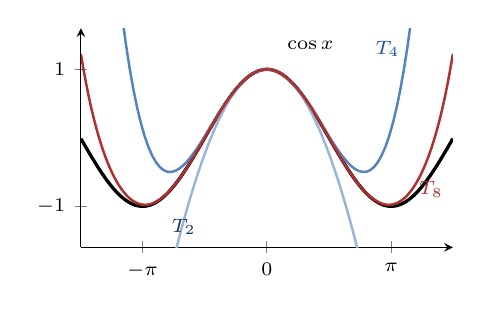
\begin{tikzpicture}
\begin{axis}[nfig, xmin=-4.7, xmax=4.7, ymin=-1.6, ymax=1.6,
  xtick={-3.1416,0,3.1416}, xticklabels={$-\pi$,$0$,$\pi$}, ytick={-1,1}, xlabel={}]
  \addplot[black, very thick, domain=-4.7:4.7, samples=200] {cos(deg(x))};
  \addplot[figB!45, domain=-4.7:4.7, samples=100] {1-x^2/2};
  \addplot[figB!75, domain=-4.7:4.7, samples=100] {1-x^2/2+x^4/24};
  \addplot[figR, domain=-4.7:4.7, samples=140] {1-x^2/2+x^4/24-x^6/720+x^8/40320};
  \node[font=\scriptsize, figB!60!black] at (axis cs:-2.1,-1.30) {$T_2$};
  \node[font=\scriptsize, figB!90!black] at (axis cs:3.05,1.30) {$T_4$};
  \node[font=\scriptsize, figR] at (axis cs:4.15,-0.75) {$T_8$};
  \node[font=\scriptsize] at (axis cs:1.1,1.35) {$\cos x$};
\end{axis}
\end{tikzpicture}%
\hfill
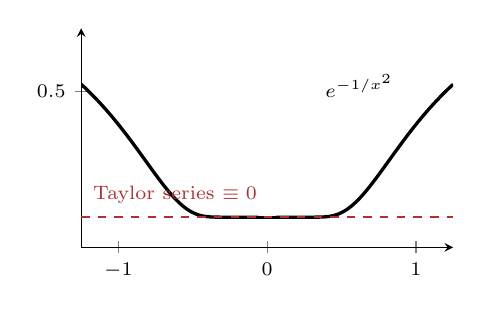
\begin{tikzpicture}
\begin{axis}[nfig, xmin=-1.25, xmax=1.25, ymin=-0.12, ymax=0.75,
  xtick={-1,0,1}, ytick={0.5}, xlabel={}]
  \addplot[black, very thick, domain=0.06:1.25, samples=250] {exp(-1/(x*x))};
  \addplot[black, very thick, domain=-1.25:-0.06, samples=250] {exp(-1/(x*x))};
  \addplot[black, very thick] coordinates {(-0.06,0.0000000001) (0.06,0.0000000001)};
  \addplot[figR, dashed, thick, domain=-1.25:1.25] {0};
  \node[font=\scriptsize] at (axis cs:0.62,0.52) {$e^{-1/x^2}$};
  \node[font=\scriptsize, figR] at (axis cs:-0.62,0.09) {Taylor series $\equiv 0$};
\end{axis}
\end{tikzpicture}\figcap{The two extremes of \S 31. Left: $T_2, T_4, T_8$ hug $\cos x$ order by order --- the remainder dies everywhere. Right: $e^{-1/x^2}$ and its Taylor series (dashed, identically $0$) are visually indistinguishable near the origin --- infinitely flat --- yet equal only at the single point $x = 0$.}
\end{center}


% ============================================================================
% CHAPTER 6: INTEGRATION
% ============================================================================

\chapter{Integration}

We now define Riemann integrals, discuss their properties, and prove the Fundamental Theorem of Calculus --- finally repaying the credit taken since \S 15.

% ============================================================================
% SECTION 32: THE RIEMANN INTEGRAL
% ============================================================================

\section{The Definition of the Riemann Integral}

Let $f: [a,b] \to \mathbb{R}$ be a function --- not necessarily continuous. We want to understand when $\int_a^b f(x)\,dx$ exists, and how to define it rigorously from what we have learned. Geometrically, it should be the area under the graph --- so we have the notion of the integral, right? \textbf{No.} The problem: \emph{what is area?} We only know how to compute areas of simple regions --- rectangles, triangles, trapezoids. The idea, as always in this course: approximate the complicated by the simple, and take a limit. \emph{The limit is the key.}

\subsection{Darboux Sums and the Darboux Integral}

\begin{defbox}[Sup and Inf over a Set; Partitions; Upper and Lower Sums]
Suppose $f$ is \emph{bounded} on $[a,b]$. For any subset $S \subseteq [a,b]$, define
\[
M(f, S) = \sup\{ f(x) \mid x \in S \}, \qquad m(f, S) = \inf\{ f(x) \mid x \in S \}
\]
(finite, by boundedness; max and min values may not exist, which is why we use $\sup$ and $\inf$). A \textbf{partition} of $[a,b]$ is a division into $n$ subintervals,
\[
P: \quad a = t_0 < t_1 < \cdots < t_n = b.
\]
For each partition define the \textbf{upper sum} and \textbf{lower sum}
\[
U(f, P) = \sum_{k=1}^n M\bigl(f, [t_{k-1}, t_k]\bigr)\,(t_k - t_{k-1}), \qquad
L(f, P) = \sum_{k=1}^n m\bigl(f, [t_{k-1}, t_k]\bigr)\,(t_k - t_{k-1})
\]
--- geometrically, sums of areas of rectangles circumscribing and inscribed in the region under the graph. If the integral exists (whatever it is), it should clearly satisfy $L(f,P) \leq \int_a^b f \leq U(f,P)$.
\end{defbox}

\begin{defbox}[Darboux Integrals]
The \textbf{Darboux upper integral} and \textbf{lower integral} are
\[
U(f) = \inf\{ U(f,P) \mid P \text{ a partition of } [a,b] \}, \quad
L(f) = \sup\{ L(f,P) \mid P \text{ a partition of } [a,b] \}.
\]
$f$ is called \textbf{Darboux integrable} if $L(f) = U(f)$, and then $\int_a^b f\,dx$ is defined to be this common value.
\end{defbox}

\begin{center}
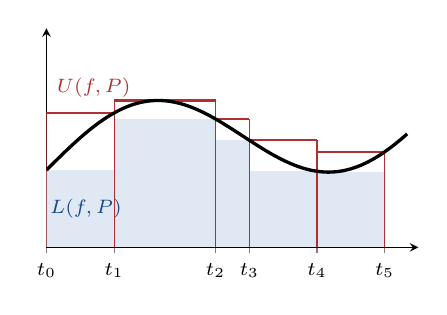
\begin{tikzpicture}
\begin{axis}[nfig, xmin=0, xmax=3.3, ymin=0, ymax=1.7,
  xtick={0,0.6,1.5,1.8,2.4,3},
  xticklabels={$t_0$,$t_1$,$t_2$,$t_3$,$t_4$,$t_5$}, ytick=\empty, xlabel={}]
  \addplot[draw=none, fill=figB!14] coordinates {(0,0) (0,0.600) (0.6,0.600) (0.6,0)};
  \addplot[draw=none, fill=figB!14] coordinates {(0.6,0) (0.6,0.996) (1.5,0.996) (1.5,0)};
  \addplot[draw=none, fill=figB!14] coordinates {(1.5,0) (1.5,0.831) (1.8,0.831) (1.8,0)};
  \addplot[draw=none, fill=figB!14] coordinates {(1.8,0) (1.8,0.590) (2.4,0.590) (2.4,0)};
  \addplot[draw=none, fill=figB!14] coordinates {(2.4,0) (2.4,0.584) (3,0.584) (3,0)};
  \addplot[figR, thick] coordinates {(0,1.043) (0.6,1.043)};
  \addplot[figR, thick] coordinates {(0.6,1.140) (1.5,1.140)};
  \addplot[figR, thick] coordinates {(1.5,0.996) (1.8,0.996)};
  \addplot[figR, thick] coordinates {(1.8,0.831) (2.4,0.831)};
  \addplot[figR, thick] coordinates {(2.4,0.741) (3,0.741)};
  \addplot[figR, thin] coordinates {(0,0) (0,1.043)};
  \addplot[figR, thin] coordinates {(0.6,0) (0.6,1.140)};
  \addplot[figR, thin] coordinates {(1.5,0) (1.5,1.140)};
  \addplot[figR, thin] coordinates {(1.8,0) (1.8,0.996)};
  \addplot[figR, thin] coordinates {(2.4,0) (2.4,0.831)};
  \addplot[figR, thin] coordinates {(3,0) (3,0.741)};
  \addplot[black, domain=0:3.2, samples=140, very thick] {0.6+0.4*sin(deg(1.8*x))+0.15*x};
  \node[font=\scriptsize, figR] at (axis cs:0.42,1.24) {$U(f,P)$};
  \node[font=\scriptsize, figB!80!black] at (axis cs:0.35,0.30) {$L(f,P)$};
\end{axis}
\end{tikzpicture}%
\hfill
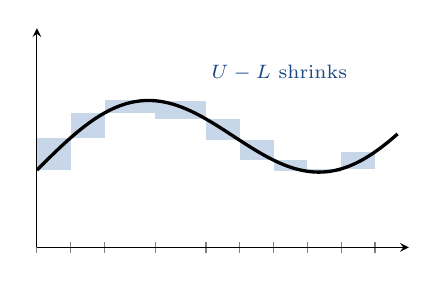
\begin{tikzpicture}
\begin{axis}[nfig, xmin=0, xmax=3.3, ymin=0, ymax=1.7,
  xtick={0,0.3,0.6,1.05,1.5,1.8,2.1,2.4,2.7,3},
  xticklabels={,,,,,,,,,}, ytick=\empty, xlabel={}]
  \addplot[draw=none, fill=figB!25] coordinates {(0,0.600) (0.3,0.600) (0.3,0.851) (0,0.851)};
  \addplot[draw=none, fill=figB!25] coordinates {(0.3,0.851) (0.6,0.851) (0.6,1.043) (0.3,1.043)};
  \addplot[draw=none, fill=figB!25] coordinates {(0.6,1.043) (1.05,1.043) (1.05,1.140) (0.6,1.140)};
  \addplot[draw=none, fill=figB!25] coordinates {(1.05,0.996) (1.5,0.996) (1.5,1.137) (1.05,1.137)};
  \addplot[draw=none, fill=figB!25] coordinates {(1.5,0.831) (1.8,0.831) (1.8,0.996) (1.5,0.996)};
  \addplot[draw=none, fill=figB!25] coordinates {(1.8,0.677) (2.1,0.677) (2.1,0.831) (1.8,0.831)};
  \addplot[draw=none, fill=figB!25] coordinates {(2.1,0.590) (2.4,0.590) (2.4,0.677) (2.1,0.677)};
  \addplot[draw=none, fill=figB!25] coordinates {(2.4,0.584) (2.7,0.584) (2.7,0.609) (2.4,0.609)};
  \addplot[draw=none, fill=figB!25] coordinates {(2.7,0.609) (3,0.609) (3,0.741) (2.7,0.741)};
  \addplot[black, domain=0:3.2, samples=140, very thick] {0.6+0.4*sin(deg(1.8*x))+0.15*x};
  \node[font=\scriptsize, figB!80!black] at (axis cs:2.15,1.35) {$U - L$ shrinks};
\end{axis}
\end{tikzpicture}\figcap{Left: an uneven partition $P$; the upper sum (red outline) and lower sum (blue fill) trap the curve. Right: a refinement of $P$ --- four more points inserted --- and the gap $U - L$ (shaded) shrinks subinterval by subinterval: the Refinement Lemma in one picture.}
\end{center}


\begin{exbox}[The identity function]
Show $f(x) = x$ is Darboux integrable on $[0,1]$ and $\int_0^1 x\,dx = \tfrac12$. (We know the value from the Fundamental Theorem --- but here we must prove it \emph{from the definition}.)

\emph{Idea:} find partitions for which $U(f,P)$ and $L(f,P)$ come close to a common value $I$. Take the equal division $P_n: t_k = \tfrac kn$. On $[t_{k-1}, t_k]$, $f = x$ is increasing, so its sup is $\tfrac kn$ and inf is $\tfrac{k-1}{n}$:
\[
U(f, P_n) = \sum_{k=1}^n \frac kn \cdot \frac1n = \frac{1}{n^2}\, \frac{n(n+1)}{2} = \frac12\left(1 + \frac1n\right),
\quad
L(f, P_n) = \frac{1}{n^2}\, \frac{(n-1)n}{2} = \frac12\left(1 - \frac1n\right).
\]
Since $U(f)$ is an infimum over \emph{all} partitions, $U(f) \leq U(f, P_n) = \tfrac12(1 + \tfrac1n)$ for every $n$; letting $n \to \infty$, $U(f) \leq \tfrac12$. Similarly $L(f) \geq \tfrac12$. Combined with the theorem below ($L(f) \leq U(f)$),
\[
\frac12 \leq L(f) \leq U(f) \leq \frac12,
\]
forcing equality: $f$ is integrable with $\int_0^1 x\,dx = \tfrac12$. \hfill $\blacksquare$
\end{exbox}

\begin{exbox}[A step function]
Show $g: [0,2] \to \mathbb{R}$, $g(x) = 1$ for $x \in [0,1)$ and $g(x) = 0$ for $x \in [1,2]$, is Darboux integrable. Given $\varepsilon > 0$, isolate the jump in a short subinterval: take
\[
P: \quad 0 < 1 - \tfrac\varepsilon2 < 1 < 2.
\]
On $[0, 1-\tfrac\varepsilon2]$: $M = m = 1$. On $[1-\tfrac\varepsilon2, 1]$: $M = 1$, $m = 0$ (the value at $1$). On $[1,2]$: $M = m = 0$. So
\[
U(g,P) = \left(1 - \tfrac\varepsilon2\right) + \tfrac\varepsilon2 = 1, \qquad L(g,P) = 1 - \tfrac\varepsilon2,
\]
and $U(g,P) - L(g,P) = \tfrac\varepsilon2 < \varepsilon$. By the Cauchy criterion below, $g$ is integrable; and since $L(g) \geq 1 - \tfrac\varepsilon2$ for every $\varepsilon$ while $U(g) \leq 1$, the integral is $\int_0^2 g = 1$. A jump discontinuity does not destroy integrability. \hfill $\blacksquare$
\end{exbox}

\begin{exbox}[The Dirichlet function is not integrable]
Let $f(x) = 1$ for $x \in \mathbb{Q}$, $f(x) = 0$ for $x \notin \mathbb{Q}$. Then $f$ is \emph{not} integrable on $[0,1]$: every subinterval $[t_{k-1}, t_k]$ of every partition contains both rationals and irrationals (density of both, \S 4 and \S 17), so
\[
M\bigl(f, [t_{k-1},t_k]\bigr) = 1, \qquad m\bigl(f, [t_{k-1},t_k]\bigr) = 0
\]
always. Hence $U(f,P) = 1$ and $L(f,P) = 0$ for \emph{every} partition, giving $U(f) = 1 \neq 0 = L(f)$. \hfill $\blacksquare$
\end{exbox}

\subsection{Lower Is at Most Upper}

\begin{thmbox}[Lower Integral at Most Upper Integral]
For every bounded $f: [a,b] \to \mathbb{R}$: \quad $L(f) \leq U(f)$.
\end{thmbox}

Is this obvious? Maybe not: $L(f)$ and $U(f)$ are a sup and an inf over \emph{different} competitions. The proof goes through two lemmas.

\begin{lembox}[Refinement Lemma]
Let $P, Q$ be partitions of $[a,b]$ with $Q$ a \textbf{refinement} of $P$ (every cut point of $P$ is a cut point of $Q$). Then
\[
L(f, P) \leq L(f, Q) \leq U(f, Q) \leq U(f, P).
\]
\end{lembox}

\begin{proof}
The middle inequality holds for any single partition, since $m \leq M$ on each subinterval. For the outer ones, it suffices (by induction on the number of added points) to add \emph{one} cut point $c$ to one subinterval $[t_{k-1}, t_k]$. The sup over a subset is at most the sup over the whole:
\[
M\bigl(f, [t_{k-1}, c]\bigr),\ M\bigl(f, [c, t_k]\bigr) \ \leq\ M\bigl(f, [t_{k-1}, t_k]\bigr),
\]
so
\[
M(f,[t_{k-1},c])(c - t_{k-1}) + M(f,[c,t_k])(t_k - c) \leq M(f,[t_{k-1},t_k])(t_k - t_{k-1}),
\]
and summing over the (unchanged) other subintervals, $U(f,Q) \leq U(f,P)$. Dually, infima over subsets are $\geq$, giving $L(f,Q) \geq L(f,P)$.
\end{proof}

\begin{lembox}[Cross Lemma]
For \emph{any} two partitions $P, Q$ (with no relation between them):
\[
L(f, P) \leq U(f, Q).
\]
\end{lembox}

\begin{proof}
The trick is a middle stepping-stone: combine $P$ and $Q$ into the common refinement $P \cup Q$ (all cut points of both). It refines both, so by the Refinement Lemma twice:
\[
L(f,P) \leq L(f, P\cup Q) \leq U(f, P \cup Q) \leq U(f, Q),
\]
the middle inequality being the single-partition fact $m \leq M$.
\end{proof}

\begin{proof}[Proof of the Theorem]
Fix any partition $Q$. By the Cross Lemma, $U(f,Q)$ is an upper bound for \emph{all} the lower sums, so
\[
L(f) = \sup_P L(f,P) \leq U(f, Q).
\]
Now $L(f)$ is a lower bound for all the upper sums, so
\[
L(f) \leq \inf_Q U(f,Q) = U(f). \qedhere
\]
\end{proof}

\subsection{The Cauchy Criterion for Integrability}

\begin{thmbox}[Cauchy Criterion]
A bounded $f: [a,b] \to \mathbb{R}$ is Darboux integrable if and only if for every $\varepsilon > 0$ there exists a partition $P$ such that
\[
U(f, P) - L(f, P) < \varepsilon.
\]
\end{thmbox}

This is convenient: we may pick a \emph{special} partition, usually the equal division, as in the examples above.

\begin{proof}
($\Rightarrow$) Suppose $f$ is integrable. Given $\varepsilon$, by the characterizations of sup and inf there are partitions $P, Q$ with
\[
L(f, P) \geq L(f) - \frac\varepsilon2, \qquad U(f, Q) \leq U(f) + \frac\varepsilon2.
\]
Pass to the common refinement $P \cup Q$: by the Refinement Lemma the two estimates persist,
\[
L(f, P\cup Q) \geq L(f) - \frac\varepsilon2, \qquad U(f, P\cup Q) \leq U(f) + \frac\varepsilon2,
\]
and since $L(f) = U(f)$, subtracting gives $U(f, P\cup Q) - L(f, P\cup Q) \leq \varepsilon$.

($\Leftarrow$) For any such $P$,
\[
U(f) - L(f) \leq U(f,P) - L(f,P) < \varepsilon.
\]
Since $\varepsilon$ is arbitrary, $U(f) - L(f) \leq 0$; combined with $U(f) - L(f) \geq 0$ (previous theorem), $U(f) = L(f)$: integrable.
\end{proof}

In computations one usually runs a whole \emph{sequence} of partitions and takes limits --- as in the identity-function example above. The following packages that pattern once and for all, value included:

\begin{propbox}[Sequential Criterion with Value (HW)]
Let $f$ be bounded on $[a,b]$, and suppose there are sequences $(U_n)$, $(L_n)$ of upper and lower Darboux sums of $f$ with $U_n - L_n \to 0$. Then $f$ is integrable and
\[
\int_a^b f\,dx = \lim_{n\to\infty} U_n = \lim_{n\to\infty} L_n.
\]
\end{propbox}

\begin{proof}
Every upper sum bounds $U(f)$ from above and every lower sum bounds $L(f)$ from below, so for each $n$,
\[
L_n \leq L(f) \leq U(f) \leq U_n, \qquad \text{hence} \qquad 0 \leq U(f) - L(f) \leq U_n - L_n \to 0,
\]
forcing $U(f) = L(f)$: $f$ is integrable, with $\int_a^b f$ trapped in every $[L_n, U_n]$. Then
\[
0 \leq U_n - \int_a^b f \leq U_n - L_n \to 0
\qquad \text{and} \qquad
0 \leq \int_a^b f - L_n \leq U_n - L_n \to 0,
\]
so both sequences converge to the integral by squeezing.
\end{proof}

For example, the equal partitions for $f(x) = x^3$ on $[0, b]$ give (via $\sum_{k=1}^n k^3 = \tfrac{n^2(n+1)^2}{4}$, proved by induction in \S 1)
\[
U_n = \frac{b^4 (n+1)^2}{4 n^2}, \qquad L_n = \frac{b^4 (n-1)^2}{4 n^2}, \qquad U_n - L_n = \frac{b^4}{n} \to 0,
\]
so $x^3$ is integrable on $[0,b]$ with $\int_0^b x^3\,dx = \lim U_n = \tfrac{b^4}{4}$ --- no separate sup/inf bookkeeping needed.

\subsection{Riemann Sums and the Riemann Integral}

\begin{defbox}[Mesh; Riemann Sums; Riemann Integrability]
For a partition $P$, define its \textbf{mesh} by $\operatorname{mesh}(P) = \max\{ t_k - t_{k-1} \}$ (for the equal partition into $n$ pieces, $\operatorname{mesh} = \tfrac{b-a}{n}$). For bounded $f$, a \textbf{Riemann sum} associated with $P$ is
\[
S = \sum_{k=1}^n f(x_k)\,(t_k - t_{k-1}), \qquad x_k \in [t_{k-1}, t_k] \text{ arbitrary}
\]
--- compare with $U(f,P)$ and $L(f,P)$, which bracket every such $S$. $f$ is called \textbf{Riemann integrable} if there exists a value $r$ such that: for every $\varepsilon > 0$ there is $\delta > 0$ such that for every partition $P$ with $\operatorname{mesh}(P) < \delta$ and every Riemann sum $S$ associated with $P$,
\[
|S - r| < \varepsilon.
\]
The value $r$ is the \textbf{Riemann integral} of $f$.
\end{defbox}

\begin{center}
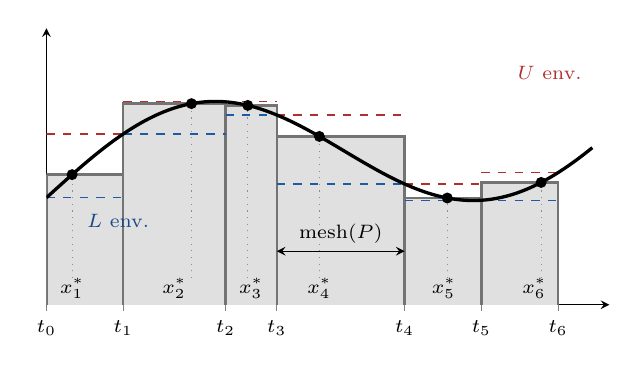
\begin{tikzpicture}
\begin{axis}[nfig, width=0.72\textwidth, height=0.42\textwidth,
  xmin=0, xmax=3.3, ymin=0, ymax=1.55,
  xtick={0,0.45,1.05,1.35,2.1,2.55,3},
  xticklabels={$t_0$,$t_1$,$t_2$,$t_3$,$t_4$,$t_5$,$t_6$}, ytick=\empty, xlabel={}]
  \addplot[draw=black!55, fill=black!12] coordinates {(0,0) (0,0.7292) (0.45,0.7292) (0.45,0)};
  \addplot[draw=black!55, fill=black!12] coordinates {(0.45,0) (0.45,1.1272) (1.05,1.1272) (1.05,0)};
  \addplot[draw=black!55, fill=black!12] coordinates {(1.05,0) (1.05,1.1173) (1.35,1.1173) (1.35,0)};
  \addplot[draw=black!55, fill=black!12] coordinates {(1.35,0) (1.35,0.9434) (2.1,0.9434) (2.1,0)};
  \addplot[draw=black!55, fill=black!12] coordinates {(2.1,0) (2.1,0.5981) (2.55,0.5981) (2.55,0)};
  \addplot[draw=black!55, fill=black!12] coordinates {(2.55,0) (2.55,0.6854) (3,0.6854) (3,0)};
  \addplot[figR, dashed, thin] coordinates {(0,0.9572) (0.45,0.9572)};
  \addplot[figR, dashed, thin] coordinates {(0.45,1.1396) (1.05,1.1396)};
  \addplot[figR, dashed, thin] coordinates {(1.05,1.1373) (1.35,1.1373)};
  \addplot[figR, dashed, thin] coordinates {(1.35,1.0637) (2.1,1.0637)};
  \addplot[figR, dashed, thin] coordinates {(2.1,0.6766) (2.55,0.6766)};
  \addplot[figR, dashed, thin] coordinates {(2.55,0.7409) (3,0.7409)};
  \addplot[figB, dashed, thin] coordinates {(0,0.6000) (0.45,0.6000)};
  \addplot[figB, dashed, thin] coordinates {(0.45,0.9572) (1.05,0.9572)};
  \addplot[figB, dashed, thin] coordinates {(1.05,1.0637) (1.35,1.0637)};
  \addplot[figB, dashed, thin] coordinates {(1.35,0.6766) (2.1,0.6766)};
  \addplot[figB, dashed, thin] coordinates {(2.1,0.5840) (2.55,0.5840)};
  \addplot[figB, dashed, thin] coordinates {(2.55,0.5855) (3,0.5855)};
  \addplot[black, domain=0:3.2, samples=140, very thick] {0.6+0.4*sin(deg(1.8*x))+0.15*x};
  \addplot[only marks, mark=*, mark size=1.5pt, black] coordinates
    {(0.15,0.7292) (0.85,1.1272) (1.18,1.1173) (1.6,0.9434) (2.35,0.5981) (2.9,0.6854)};
  \node[font=\scriptsize] at (axis cs:0.15,0.09) {$x_1^*$};
  \node[font=\scriptsize] at (axis cs:0.75,0.09) {$x_2^*$};
  \node[font=\scriptsize] at (axis cs:1.20,0.09) {$x_3^*$};
  \node[font=\scriptsize] at (axis cs:1.6,0.09) {$x_4^*$};
  \node[font=\scriptsize] at (axis cs:2.33,0.09) {$x_5^*$};
  \node[font=\scriptsize] at (axis cs:2.86,0.09) {$x_6^*$};
  \draw[black!45, thin, dotted] (axis cs:0.15,0.15) -- (axis cs:0.15,0.7292);
  \draw[black!45, thin, dotted] (axis cs:0.85,0.15) -- (axis cs:0.85,1.1272);
  \draw[black!45, thin, dotted] (axis cs:1.18,0.15) -- (axis cs:1.18,1.1173);
  \draw[black!45, thin, dotted] (axis cs:1.6,0.15) -- (axis cs:1.6,0.9434);
  \draw[black!45, thin, dotted] (axis cs:2.35,0.15) -- (axis cs:2.35,0.5981);
  \draw[black!45, thin, dotted] (axis cs:2.9,0.15) -- (axis cs:2.9,0.6854);
  \draw[stealth-stealth, thin] (axis cs:1.35,0.30) -- (axis cs:2.1,0.30);
  \node[font=\scriptsize] at (axis cs:1.725,0.40) {$\operatorname{mesh}(P)$};
  \node[font=\scriptsize, figR] at (axis cs:2.95,1.30) {$U$ env.};
  \node[font=\scriptsize, figB!80!black] at (axis cs:0.42,0.47) {$L$ env.};
\end{axis}
\end{tikzpicture}\figcap{A Riemann sum: both choices are arbitrary --- the partition points $t_k$ (unequal lengths; $\operatorname{mesh}(P)$ is the widest) and the tags $x_k^*$ inside each piece, with rectangle heights $f(x_k^*)$, neither sup nor inf. Dashed red and blue mark the Darboux envelopes on each subinterval: every Riemann sum is squeezed, $L(f,P) \leq S \leq U(f,P)$ --- the mechanism behind the equivalence theorem below.}
\end{center}


One difficulty in \emph{using} this definition: we need a candidate value $r$ before we can check anything --- whereas the Darboux definition asks only for the sup and inf to meet. Fortunately:

\begin{thmbox}[Equivalence of the Two Integrals]
\begin{enumerate}[label=(\arabic*)]
    \item $f: [a,b] \to \mathbb{R}$ is Riemann integrable if and only if it is Darboux integrable (and the values agree).
    \item (Mesh form of the Cauchy criterion) $f$ is Darboux integrable if and only if for every $\varepsilon > 0$ there is $\delta > 0$ such that \emph{every} partition with $\operatorname{mesh}(P) < \delta$ satisfies $U(f,P) - L(f,P) < \varepsilon$.
\end{enumerate}
\end{thmbox}

These were stated without proof in lecture (the proofs take too much time; see the book for details). The essential difference between the two notions is that Riemann's requires a limit in the $\varepsilon$-$\delta$ sense over the mesh, which (2) supplies on the Darboux side. From now on, ``integrable'' means either.

\begin{thmbox}[Continuous Functions Are Integrable]
If $f: [a,b] \to \mathbb{R}$ is continuous ($a, b$ finite), then $f$ is integrable.
\end{thmbox}

\begin{proof}
We show $f$ is Darboux integrable via the Cauchy criterion. The key: since $f$ is continuous on the closed bounded $[a,b]$, it is \emph{uniformly continuous} (\S 19 --- this is exactly the application promised there). So for every $\varepsilon > 0$ there exists $\delta > 0$ such that
\[
|x - y| < \delta \implies |f(x) - f(y)| < \frac{\varepsilon}{b-a}.
\]
Choose $n$ so large that $\tfrac{b-a}{n} < \delta$, and let $P$ be the equal partition into $n$ subintervals. On each $[t_{k-1}, t_k]$, any two points are within $\delta$, so any two values of $f$ differ by less than $\tfrac{\varepsilon}{b-a}$; taking suprema over pairs,
\[
M\bigl(f,[t_{k-1},t_k]\bigr) - m\bigl(f,[t_{k-1},t_k]\bigr) \leq \frac{\varepsilon}{b-a}.
\]
Therefore
\[
U(f,P) - L(f,P) = \sum_{k=1}^n \bigl(M_k - m_k\bigr)\,\frac{b-a}{n} \leq \sum_{k=1}^n \frac{\varepsilon}{b-a}\cdot\frac{b-a}{n} = \varepsilon. \qedhere
\]
\end{proof}

% ============================================================================
% SECTION 33: PROPERTIES OF THE RIEMANN INTEGRAL
% ============================================================================

\section{Properties of the Riemann Integral}

It is often not easy to check integrability from the definitions --- we need properties.

\begin{thmbox}[Monotonic Functions Are Integrable]
If $f: [a,b] \to \mathbb{R}$ is monotonic, then $f$ is integrable. (Note $f$ need not be continuous --- though one can prove a monotonic function has at most countably many discontinuities, so it is not too bad.)
\end{thmbox}

\begin{proof}
Say $f$ is increasing (the decreasing case is symmetric). Take the equal partition $P$, so $t_k - t_{k-1} = \tfrac{b-a}{n}$. By monotonicity, the sup and inf on each subinterval are attained at the endpoints:
\[
M\bigl(f, [t_{k-1},t_k]\bigr) = f(t_k), \qquad m\bigl(f, [t_{k-1},t_k]\bigr) = f(t_{k-1}).
\]
So the difference of the sums \emph{telescopes}:
\[
U(f,P) - L(f,P) = \sum_{k=1}^n \bigl( f(t_k) - f(t_{k-1}) \bigr)\, \frac{b-a}{n} = \bigl( f(b) - f(a) \bigr)\, \frac{b-a}{n}.
\]
For any $\varepsilon > 0$, take $n$ large enough that this is $< \varepsilon$: the Cauchy criterion applies. Done!
\end{proof}

\begin{thmbox}[Linearity]
If $f, g: [a,b] \to \mathbb{R}$ are integrable, then:
\begin{enumerate}[label=(\arabic*)]
    \item for any constant $c$, $cf$ is integrable and $\int_a^b cf = c\int_a^b f$;
    \item $f + g$ is integrable and
    \[
    \int_a^b (f + g)\,dx = \int_a^b f\,dx + \int_a^b g\,dx.
    \]
\end{enumerate}
\end{thmbox}

\begin{proof}
(1) For $c \geq 0$: $U(cf, P) = c\,U(f,P)$ and $L(cf,P) = c\,L(f,P)$, so the Cauchy criterion and the value transfer directly. For $c < 0$, multiplying by $c$ \emph{swaps} sup and inf: $U(cf,P) = c\,L(f,P)$ and $L(cf,P) = c\,U(f,P)$; the criterion and value again follow.

(2) Here the Darboux approach meets a difficulty: on a subinterval $I$,
\[
M(f+g, I) \ \neq\ M(f,I) + M(g,I) \quad \text{in general}
\]
(the two functions may peak at different points) --- only the inequalities
\[
M(f+g, I) \leq M(f,I) + M(g,I), \qquad m(f+g, I) \geq m(f,I) + m(g,I)
\]
hold (for Riemann sums, by contrast, additivity is exact --- which is why the lecture remarked that Riemann's definition handles (2) more easily). Summing the inequalities over any partition $P$:
\[
L(f,P) + L(g,P) \leq L(f+g, P) \leq U(f+g, P) \leq U(f,P) + U(g,P).
\]
Given $\varepsilon$, choose partitions with $U(f,\cdot) - L(f,\cdot) < \tfrac\varepsilon2$ and $U(g,\cdot) - L(g,\cdot) < \tfrac\varepsilon2$, and pass to their common refinement $P$; then the outer quantities above are within $\varepsilon$ of each other, so $U(f+g,P) - L(f+g,P) < \varepsilon$: $f+g$ is integrable. Moreover the display traps both $\int(f+g)$ and $\int f + \int g$ in the same interval of length $< \varepsilon$; as $\varepsilon$ is arbitrary, they are equal.
\end{proof}

\begin{thmbox}[Monotonicity of the Integral]
If $f, g$ are integrable on $[a,b]$ and $f(x) \leq g(x)$ for all $x$, then
\[
\int_a^b f\,dx \leq \int_a^b g\,dx.
\]
\end{thmbox}

\begin{proof}
First: if $h \leq 0$ is integrable, then $\int_a^b h \leq 0$, since already $U(h, P) \leq 0$ for every $P$ (each $M(h, \cdot) \leq 0$), and the integral is $\leq$ every upper sum. Now write $f = g + (f - g)$ with $f - g \leq 0$ integrable (linearity):
\[
\int_a^b f = \int_a^b g + \int_a^b (f - g) \leq \int_a^b g. \qedhere
\]
\end{proof}

\begin{thmbox}[Absolute Values]
If $f: [a,b] \to \mathbb{R}$ is integrable, then $|f|$ is integrable, and
\[
\left| \int_a^b f\,dx \right| \leq \int_a^b |f|\,dx.
\]
\end{thmbox}

\begin{proof}
Which definition to use? Riemann sums are awkward here; Darboux works. The key observation: on any subinterval $I$,
\[
M(|f|, I) - m(|f|, I) \ \leq\ M(f, I) - m(f, I)
\]
--- \emph{taking absolute values decreases the variation}. Indeed, for any $x, y \in I$, the reverse triangle inequality gives
\[
\bigl| |f(x)| - |f(y)| \bigr| \leq |f(x) - f(y)| \leq M(f,I) - m(f,I),
\]
and taking the supremum over pairs $x, y$ on the left yields exactly $M(|f|,I) - m(|f|,I)$. Consequently $U(|f|,P) - L(|f|,P) \leq U(f,P) - L(f,P)$ for every partition, and the Cauchy criterion transfers from $f$ to $|f|$.

For the inequality: $\pm f \leq |f|$, so by monotonicity and linearity, $\pm \int_a^b f \leq \int_a^b |f|$, which is the claim.
\end{proof}

\begin{rembox}[Warning]
The converse fails: for $f = 1$ on $\mathbb{Q}$ and $f = -1$ off $\mathbb{Q}$, the function $|f| \equiv 1$ is integrable on $[0,1]$, but $f$ is not (the Dirichlet argument verbatim: $U(f,P) = 1$, $L(f,P) = -1$ always).
\end{rembox}

\begin{thmbox}[Additivity over Subintervals]
Let $a < c < b$. If $f$ is integrable on $[a,c]$ and on $[c,b]$, then $f$ is integrable on $[a,b]$, and
\[
\int_a^b f\,dx = \int_a^c f\,dx + \int_c^b f\,dx.
\]
\end{thmbox}

\begin{proof}
Given $\varepsilon > 0$, take partitions $P_1$ of $[a,c]$ and $P_2$ of $[c,b]$ with $U - L < \tfrac\varepsilon2$ on each. Their concatenation $P = P_1 \cup P_2$ is a partition of $[a,b]$ (containing $c$ as a cut point), and upper/lower sums split along $c$:
\[
U(f, P) = U(f, P_1) + U(f, P_2), \qquad L(f,P) = L(f,P_1) + L(f,P_2),
\]
so $U(f,P) - L(f,P) < \varepsilon$: integrable on $[a,b]$. The same splitting traps $\int_a^b f$ and $\int_a^c f + \int_c^b f$ between the same bounds within $\varepsilon$, forcing equality.
\end{proof}

The converse direction --- that integrability passes \emph{down} to subintervals --- is what makes splitting a given integral legal in the first place:

\begin{propbox}[Restriction to Subintervals (HW)]
If $f$ is integrable on $[a,b]$, then $f$ is integrable on every interval $[c,d] \subseteq [a,b]$.
\end{propbox}

\begin{proof}
Given $\varepsilon > 0$, the Cauchy criterion (\S 32) provides a partition $P$ of $[a,b]$ with $U(f,P) - L(f,P) < \varepsilon$. Refine to $P^* = P \cup \{c, d\}$; by the Refinement Lemma the difference only shrinks:
\[
U(f, P^*) - L(f, P^*) < \varepsilon.
\]
The points of $P^*$ lying in $[c,d]$ form a partition $P_2$ of $[c,d]$ (with $c, d$ as its endpoints), and the total difference splits along $c$ and $d$ into three blocks --- over $[a,c]$, $[c,d]$, $[d,b]$ --- each of the form $\sum (M_k - m_k)(t_k - t_{k-1}) \geq 0$. Discarding the two outer blocks,
\[
U(f, [c,d], P_2) - L(f, [c,d], P_2) \leq U(f, P^*) - L(f, P^*) < \varepsilon,
\]
and the Cauchy criterion on $[c,d]$ concludes.
\end{proof}

\begin{rembox}
Together the two results make integrability on $[a,b]$ \emph{equivalent} to integrability on both halves, and they license every splitting used later: chopping an integral along a partition (as in the FTC's telescoping, \S 34) silently invokes this proposition to know each piece $\int_{t_{k-1}}^{t_k} f$ exists.
\end{rembox}

\subsection{Positivity}

\begin{thmbox}[Vanishing Integral of a Nonnegative Function]
Suppose $f: [a,b] \to \mathbb{R}$ is continuous and $f(x) \geq 0$ for all $x \in [a,b]$. Then $\int_a^b f\,dx \geq 0$; and if
\[
\int_a^b f\,dx = 0,
\]
then $f(x) = 0$ for \emph{all} $x \in [a,b]$.
\end{thmbox}

\begin{proof}
The first statement is a special case of monotonicity ($0 \leq f$). For the second --- why is it true? Geometrically: a bump anywhere would contribute positive area. Prove it by contradiction: suppose $f(x_0) > 0$ for some $x_0 \in [a,b]$. We may assume $x_0 \in (a,b)$: if $x_0$ were an endpoint, continuity provides nearby \emph{interior} points where $f$ is still close to $f(x_0)$, hence positive --- replace $x_0$ by one of them.

By continuity at $x_0$ (with tolerance $\tfrac{f(x_0)}{2}$), there is $\varepsilon > 0$ small enough that $[x_0 - \varepsilon, x_0 + \varepsilon] \subset [a,b]$ and, for all $x$ in this neighborhood,
\[
|f(x) - f(x_0)| < \frac{f(x_0)}{2}, \qquad \text{hence} \qquad f(x) > \frac{f(x_0)}{2}.
\]
Now split the integral (additivity over subintervals) and discard the two outer pieces, which are $\geq 0$ since $f \geq 0$:
\[
\int_a^b f\,dx = \int_a^{x_0-\varepsilon} f + \int_{x_0-\varepsilon}^{x_0+\varepsilon} f + \int_{x_0+\varepsilon}^b f
\ \geq\ \int_{x_0-\varepsilon}^{x_0+\varepsilon} f
\ \geq\ \int_{x_0-\varepsilon}^{x_0+\varepsilon} \frac{f(x_0)}{2}\,dx
= \frac{f(x_0)}{2}\cdot 2\varepsilon = f(x_0)\,\varepsilon > 0,
\]
contradicting $\int_a^b f = 0$.
\end{proof}

\begin{corbox}[Vanishing Integral of a Square]
If $f: [a,b] \to \mathbb{R}$ is continuous and $\int_a^b f^2\,dx = 0$, then $f \equiv 0$.
\end{corbox}

\begin{proof}
$f^2$ is continuous and $f^2(x) \geq 0$; the theorem gives $f^2 \equiv 0$, hence $f \equiv 0$.
\end{proof}

\begin{exbox}[Orthogonal to everything means zero]
Let $f: [a,b] \to \mathbb{R}$ be continuous, and suppose that for \emph{all} continuous $g: [a,b] \to \mathbb{R}$,
\[
\int_a^b f(x)g(x)\,dx = 0.
\]
Show $f \equiv 0$. How? Take $g = f$: then $\int_a^b f^2 = 0$, and the corollary finishes. \hfill $\blacksquare$
\end{exbox}

\begin{rembox}[Inner products on function spaces]
In $\mathbb{R}^2$, $\mathbb{R}^3$ we have orthogonality of vectors, governed by the inner product $\langle x, y \rangle = \sum_i x_i y_i$. On the space of continuous functions on $[a,b]$ --- an \emph{infinite-dimensional} vector space --- the integral supplies an inner product:
\[
\langle f, g \rangle = \int_a^b f(x)g(x)\,dx.
\]
In $\mathbb{R}^2$, a vector perpendicular to every vector must be zero; the example above is exactly the same statement for the vector space of functions, proved by the same idea (pair the vector with itself).
\end{rembox}

\subsection{Mean Value Theorems for Integrals}

\begin{thmbox}[Intermediate Value Theorem for Integrals]
Let $f: [a,b] \to \mathbb{R}$ be continuous. Then there exists at least one point $x_0 \in [a,b]$ such that
\[
f(x_0) = \frac{1}{b-a} \int_a^b f\,dx.
\]
\end{thmbox}

What does it mean? The right side is the \textbf{mean value} of $f$ over $[a,b]$: the mean value is attained --- it equals the value of $f$ at some point.

\begin{rembox}
The continuity assumption is important. Counterexample: $f: [-1,1] \to \mathbb{R}$ with $f = -1$ on $[-1, 0)$ and $f = 1$ on $[0,1]$ (a step function, integrable by \S 32). Its mean value is $0$ --- a value $f$ never takes.
\end{rembox}

\begin{proof}
Since $f$ is continuous on the closed bounded interval, the Extreme Value Theorem provides a maximum point $x_1$ and a minimum point $x_2$:
\[
f(x_1) = M = \max f, \qquad f(x_2) = m = \min f.
\]
By monotonicity of the integral, $m \leq f \leq M$ gives
\[
m(b-a) \leq \int_a^b f\,dx \leq M(b-a), \qquad \text{i.e.} \qquad m \leq \frac{1}{b-a}\int_a^b f\,dx \leq M.
\]
So the average value lies between $f(x_2)$ and $f(x_1)$. By the Intermediate Value Theorem for continuous functions (\S 18, applied between the points $x_1$ and $x_2$), some $x_0$ between them satisfies
\[
f(x_0) = \frac{1}{b-a}\int_a^b f\,dx. \qedhere
\]
\end{proof}

\begin{thmbox}[Weighted Mean Value Theorem]
Let $f, g: [a,b] \to \mathbb{R}$ be continuous with $g(x) \geq 0$ for all $x$. Then there exists $x_0 \in [a,b]$ such that
\[
\int_a^b f(x)g(x)\,dx = f(x_0) \int_a^b g(x)\,dx.
\]
This generalizes the previous theorem ($g \equiv 1$); here $g$ plays the role of a \emph{weight function}, and the left side divided by $\int g$ is the weighted average of $f$.
\end{thmbox}

\begin{proof}
The same proof. With $M = \max f$, $m = \min f$: since $g \geq 0$,
\[
m\,g(x) \leq f(x)g(x) \leq M\,g(x),
\]
and integrating (monotonicity),
\[
m \int_a^b g\,dx \leq \int_a^b fg\,dx \leq M \int_a^b g\,dx.
\]
If $\int_a^b g\,dx = 0$: then $g \equiv 0$ by the positivity theorem (continuous, nonnegative), so $fg \equiv 0$, both sides vanish, and any $x_0$ works. Otherwise divide:
\[
m \leq \frac{\int_a^b fg\,dx}{\int_a^b g\,dx} \leq M,
\]
and the Intermediate Value Theorem for $f$ (between its min and max points) supplies $x_0$. Done.
\end{proof}

The theorem places $x_0$ only in the \emph{closed} interval. That is genuinely weaker than it needs to be:

\begin{propbox}[The Witness Can Be Taken Interior (HW)]
In the Weighted Mean Value Theorem, the point can always be chosen with $x_0 \in (a,b)$, the \emph{open} interval.
\end{propbox}

\begin{proof}
If $\int_a^b g\,dx = 0$, then (as in the theorem's proof) both sides vanish for \emph{every} $x_0$; pick any interior point. So assume $\int_a^b g\,dx > 0$ and set
\[
A = \frac{\int_a^b fg\,dx}{\int_a^b g\,dx} \in [m, M].
\]
If $f$ is constant, $A = f(x_0)$ for every interior $x_0$. So assume $m < M$, and split by where $A$ sits.

\emph{Interior value} ($m < A < M$): let $x_1, x_2 \in [a,b]$ attain $f(x_1) = M$, $f(x_2) = m$ (Extreme Value Theorem); these are distinct. The IVT on the interval between them gives $x_0$ with $f(x_0) = A$, and since $A$ differs from both endpoint values, $x_0$ lies \emph{strictly} between $x_1$ and $x_2$ --- hence strictly inside $[a,b]$.

\emph{Boundary value} ($A = m$; the case $A = M$ is symmetric): then
\[
\int_a^b (f - m)\,g\,dx = \int_a^b fg\,dx - m \int_a^b g\,dx = 0,
\]
with $(f-m)g$ continuous and $\geq 0$; by the vanishing-integral theorem above, $(f - m)\,g \equiv 0$ on $[a,b]$. Since $\int_a^b g\,dx > 0$, some $x^*$ has $g(x^*) > 0$, and by continuity $g > 0$ on a whole interval $(x^* - \delta, x^* + \delta) \cap [a,b]$ of positive length. On that interval the identity $(f-m)g \equiv 0$ forces $f \equiv m$; and an interval of positive length inside $[a,b]$ certainly contains a point $x_0$ of the open $(a,b)$. There, $f(x_0) = m = A$.
\end{proof}

\begin{rembox}
All the work sits in the boundary cases $A \in \{m, M\}$, where the plain IVT route might hand back only an endpoint (if $f$ attains its extremum nowhere else). The rescue mechanism --- vanishing integral of a nonnegative continuous function forces identical vanishing, then local positivity of $g$ converts one good point into a whole subinterval --- is the same tool as ``orthogonal to everything means zero'' above. Taking $g \equiv 1$ shows the ordinary Intermediate Value Theorem for Integrals also admits an interior witness.
\end{rembox}

\begin{exbox}[Equal integrals meet]
Suppose $f, g: [a,b] \to \mathbb{R}$ are continuous and $\int_a^b f = \int_a^b g$. Show that $f(x_0) = g(x_0)$ for some $x_0 \in [a,b]$.

Consider $h = f - g$: continuous, with $\int_a^b h = 0$ by linearity --- so the mean value of $h$ is $0$. By the Intermediate Value Theorem for integrals, some $x_0$ has
\[
h(x_0) = \frac{1}{b-a}\int_a^b h\,dx = 0, \qquad \text{i.e.} \qquad f(x_0) = g(x_0).
\]
\emph{In fact $x_0$ can be found in the open interval $(a,b)$} (HW). Suppose not: $h$ has no zero in $(a,b)$. Being continuous and never zero there, $h$ keeps a constant sign on $(a,b)$ (otherwise the IVT would manufacture a zero); say $h > 0$ on $(a,b)$ (else replace $h$ by $-h$). By continuity, $h(a), h(b) \geq 0$ as limits of positive values, so $h \geq 0$ on all of $[a,b]$ --- continuous, nonnegative, with $\int_a^b h = 0$. The vanishing-integral theorem forces $h \equiv 0$, contradicting $h > 0$ on the nonempty $(a,b)$. \hfill $\blacksquare$
\end{exbox}

\subsection{Uniform Convergence and Integration Revisited}

\begin{thmbox}[Integration of Uniform Limits]
Suppose $f_n: [a,b] \to \mathbb{R}$ are continuous and converge uniformly to $f$. Then $f$ is integrable, and
\[
\int_a^b f_n\,dx \longrightarrow \int_a^b f\,dx.
\]
\end{thmbox}

\begin{proof}
By the uniform-limit theorem of \S 24, $f$ is continuous --- hence integrable, by \S 32. (This is the point that was taken on credit back in \S 25: there, integrability was part of the calculus toolkit; now it is proved.) For the convergence: given $\varepsilon > 0$, uniform convergence provides $N$ such that for $n \geq N$ and all $x \in [a,b]$,
\[
|f_n(x) - f(x)| < \frac{\varepsilon}{b-a}.
\]
Then, by linearity, the absolute-value inequality, and monotonicity,
\[
\left| \int_a^b f_n\,dx - \int_a^b f\,dx \right| = \left| \int_a^b (f_n - f)\,dx \right| \leq \int_a^b |f_n - f|\,dx \leq \int_a^b \frac{\varepsilon}{b-a}\,dx = \varepsilon. \qedhere
\]
\end{proof}

% ============================================================================
% SECTION 34: FUNDAMENTAL THEOREM OF CALCULUS
% ============================================================================

\section{Fundamental Theorem of Calculus}

The last main section --- and the moment the oldest debts of these notes are repaid.

\subsection{The First Fundamental Theorem}

\begin{thmbox}[Fundamental Theorem of Calculus I]
Assume $g: [a,b] \to \mathbb{R}$ is continuous, differentiable on $(a,b)$, and $g'$ is integrable on $[a,b]$. Then
\[
\int_a^b g'(x)\,dx = g(b) - g(a).
\]
\end{thmbox}

We all know this --- but how to \emph{prove} it? The integral $\int_a^b g'$ is defined via upper and lower sums $U(g', P)$, $L(g', P)$; the key is to trap $g(b) - g(a)$ between the \emph{same} sums.

\begin{proof}
Let $\varepsilon > 0$. Since $g'$ is integrable, the Cauchy criterion provides a partition
\[
P: \quad a = t_0 < t_1 < \cdots < t_n = b, \qquad U(g', P) - L(g', P) < \varepsilon.
\]
Telescope the increment of $g$ along the partition, and apply the \textbf{Mean Value Theorem} on each subinterval ($g$ is continuous on $[t_{k-1}, t_k]$ and differentiable inside):
\[
g(b) - g(a) = \sum_{k=1}^n \bigl( g(t_k) - g(t_{k-1}) \bigr) = \sum_{k=1}^n g'(x_k)\,(t_k - t_{k-1})
\]
for some points $x_k \in (t_{k-1}, t_k)$ --- the middle expression is a \emph{Riemann sum} for $g'$. Now bracket each term:
\[
m\bigl(g', [t_{k-1},t_k]\bigr)(t_k - t_{k-1}) \ \leq\ g'(x_k)(t_k - t_{k-1}) \ \leq\ M\bigl(g', [t_{k-1},t_k]\bigr)(t_k - t_{k-1}),
\]
and sum:
\[
L(g', P) \ \leq\ g(b) - g(a) \ \leq\ U(g', P).
\]
But also, by the definition of the Darboux integral,
\[
L(g', P) \ \leq\ \int_a^b g'\,dx \ \leq\ U(g', P).
\]
Both numbers lie in an interval of length $< \varepsilon$, so (sandwich)
\[
\left| \int_a^b g'\,dx - \bigl( g(b) - g(a) \bigr) \right| < \varepsilon.
\]
Since $\varepsilon$ is arbitrary, the difference is $0$. Done.
\end{proof}

\subsection{Integration by Parts}

Integration by parts needs a preliminary: products of integrable functions are integrable.

\begin{lembox}[Products of Integrable Functions]
If $f, g: [a,b] \to \mathbb{R}$ are integrable, then $f^2$ and $fg$ are integrable.
\end{lembox}

\begin{proof}
\emph{Step 1: $f^2$.} Let $B$ bound $|f|$. From the factorization $f(x)^2 - f(y)^2 = \bigl(f(x)+f(y)\bigr)\bigl(f(x)-f(y)\bigr)$, on any subinterval $I$,
\[
\bigl| f(x)^2 - f(y)^2 \bigr| \leq 2B\, |f(x) - f(y)| \leq 2B\bigl( M(f,I) - m(f,I) \bigr),
\]
and taking the sup over pairs, $M(f^2, I) - m(f^2, I) \leq 2B\bigl(M(f,I) - m(f,I)\bigr)$. Hence
\[
U(f^2, P) - L(f^2, P) \leq 2B\bigl( U(f,P) - L(f,P) \bigr),
\]
and the Cauchy criterion transfers from $f$ to $f^2$ (choose $P$ with $U - L < \tfrac{\varepsilon}{2B}$).

\emph{Step 2: $fg$.} Use the polarization identity
\[
fg = \frac14\Bigl( (f+g)^2 - (f-g)^2 \Bigr):
\]
$f \pm g$ are integrable (linearity), their squares are integrable (Step 1), and linear combinations of integrable functions are integrable.
\end{proof}

\begin{thmbox}[Integration by Parts]
If $u, v: [a,b] \to \mathbb{R}$ are continuous, differentiable on $(a,b)$, and $u', v'$ are integrable on $[a,b]$, then
\[
\int_a^b u(x)v'(x)\,dx = u(b)v(b) - u(a)v(a) - \int_a^b u'(x)v(x)\,dx.
\]
The point: trade the integrand $uv'$ for $u'v$, hoping it is simpler.
\end{thmbox}

\begin{proof}
By the lemma, $uv'$ and $u'v$ are integrable (each factor is integrable: $u, v$ are continuous, $u', v'$ by hypothesis). Apply FTC I to $g = uv$: by the product rule $g' = u'v + uv'$, which is integrable, so
\[
u(b)v(b) - u(a)v(a) = g(b) - g(a) = \int_a^b g'\,dx = \int_a^b u'v\,dx + \int_a^b uv'\,dx,
\]
and rearrange.
\end{proof}

\subsection{The Second Fundamental Theorem}

\begin{thmbox}[Fundamental Theorem of Calculus II]
If $f: [a,b] \to \mathbb{R}$ is bounded and integrable, then
\[
F(x) = \int_a^x f(t)\,dt
\]
is a continuous function of $x$ on $[a,b]$. If moreover $f$ is continuous at $x_0$, then $F$ is differentiable at $x_0$ with
\[
F'(x_0) = f(x_0).
\]
Likewise, $G(x) = \int_x^b f(t)\,dt$ satisfies $G'(x_0) = -f(x_0)$ (since $G = \int_a^b f - F$).
\end{thmbox}

\begin{rembox}[Orientation convention]
For $x < y$ we set $\int_y^x f = -\int_x^y f$; then additivity $\int_a^x = \int_a^y + \int_y^x$ holds for any order of the points, and the estimates below are valid regardless of the side from which $x$ approaches $x_0$.
\end{rembox}

\begin{proof}
\textbf{Continuity of $F$.} Let $M$ bound $|f|$. For any $x, y$,
\[
|F(x) - F(y)| = \left| \int_y^x f(t)\,dt \right| \leq \left| \int_y^x M\,dt \right| = M\,|x - y|,
\]
so $F$ is Lipschitz --- in particular (uniformly) continuous.

\textbf{Differentiability at a continuity point.} For $x \neq x_0$, using $\int_{x_0}^x f(x_0)\,dt = f(x_0)(x - x_0)$,
\[
\frac{F(x) - F(x_0)}{x - x_0} - f(x_0) = \frac{1}{x - x_0}\int_{x_0}^x \bigl( f(t) - f(x_0) \bigr)\,dt.
\]
Since $f$ is continuous at $x_0$: for every $\varepsilon > 0$ there is $\delta > 0$ with $|f(t) - f(x_0)| < \varepsilon$ whenever $|t - x_0| < \delta$. If $|x - x_0| < \delta$, then every $t$ between $x_0$ and $x$ also satisfies $|t - x_0| < \delta$, so
\[
\left| \frac{1}{x - x_0}\int_{x_0}^x \bigl(f(t) - f(x_0)\bigr)\,dt \right| \leq \frac{1}{|x - x_0|} \left| \int_{x_0}^x \varepsilon\,dt \right| = \varepsilon.
\]
Hence the difference quotient tends to $f(x_0)$: $F'(x_0) = f(x_0)$. Done.
\end{proof}

\begin{center}
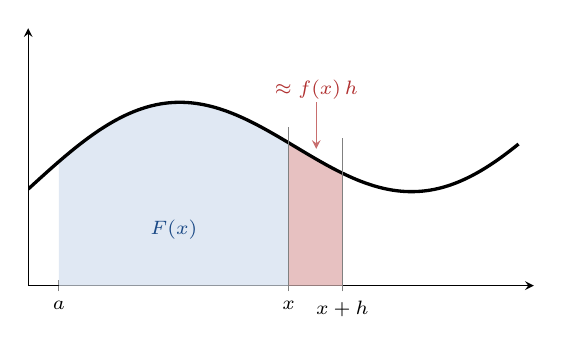
\begin{tikzpicture}
\begin{axis}[nfig, width=0.66\textwidth, height=0.40\textwidth,
  xmin=0, xmax=3.3, ymin=0, ymax=1.6,
  xtick={0.2,1.7,2.05}, xticklabels={$a$,$x$,$x+h$}, ytick=\empty, xlabel={}]
  \addplot[draw=none, fill=figB!14, domain=0.2:1.7, samples=80] {0.6+0.4*sin(deg(1.8*x))+0.15*x} \closedcycle;
  \addplot[draw=none, fill=figR!30, domain=1.7:2.05, samples=20] {0.6+0.4*sin(deg(1.8*x))+0.15*x} \closedcycle;
  \addplot[black, very thick, domain=0:3.2, samples=140] {0.6+0.4*sin(deg(1.8*x))+0.15*x};
  \draw[black!50, thin] (axis cs:1.7,0) -- (axis cs:1.7,0.988);
  \draw[black!50, thin] (axis cs:2.05,0) -- (axis cs:2.05,0.917);
  \node[font=\scriptsize, figB!80!black] at (axis cs:0.95,0.35) {$F(x)$};
  \node[font=\scriptsize, figR] at (axis cs:1.88,1.22) {$\approx f(x)\,h$};
  \draw[figR!70, -stealth, thin] (axis cs:1.88,1.14) -- (axis cs:1.88,0.85);
\end{axis}
\end{tikzpicture}\figcap{The proof in one strip: $F(x)$ is the shaded area, and the increment $F(x+h) - F(x)$ is the thin strip --- of area $f(x)\,h$ up to an error controlled by the continuity of $f$ at $x$. Dividing by $h$: $F'(x) = f(x)$.}
\end{center}


\begin{exbox}[FTC I from FTC II when the derivative is continuous (HW)]
The two halves of the FTC are not independent: if $g'$ is \emph{continuous}, FTC I follows from FTC II in three lines. Set $G(x) = \int_a^x g'(t)\,dt$. By FTC II, $G$ is continuous on $[a,b]$ and $G' = g'$ on $(a,b)$; so $G - g$ has vanishing derivative on $(a,b)$ and is constant there (\S 29), and the constancy extends to the closed interval by continuity of $G - g$. Evaluating the constant at both ends,
\[
G(b) - g(b) = G(a) - g(a) = 0 - g(a), \qquad \text{i.e.} \qquad \int_a^b g'(t)\,dt = G(b) = g(b) - g(a).
\]
\end{exbox}

\begin{rembox}
So why did FTC I get its own telescoping proof? Because its hypothesis is weaker: $g'$ need only be \emph{integrable}. Discontinuous derivatives genuinely occur (\S 28's middle rung $x^2\sin\tfrac1x$ has a derivative with no limit at $0$), and at a discontinuity point FTC II is silent about $G'$ --- the shortcut above collapses. The telescope, using only the MVT on each subinterval, never needs to differentiate $G$ at all. A theorem proved twice, under different hypotheses, is really two theorems.
\end{rembox}

\begin{exbox}[Variable limits and the chain rule]
Assume $f$ is continuous on $\mathbb{R}$. Show $G(x) = \displaystyle\int_0^{\sin x} f(t)\,dt$ is differentiable and compute $G'$.

Write $G = F \circ \sin$, where $F(u) = \int_0^u f(t)\,dt$. By FTC II, $F' = f$ everywhere (continuity of $f$); by the chain rule (\S 28),
\[
G'(x) = F'(\sin x)\cdot(\sin x)' = f(\sin x)\,\cos x. \tag*{$\blacksquare$}
\]
\end{exbox}

One step deserves scrutiny (HW): the claim ``$F' = f$ \emph{everywhere}'' --- FTC II was stated on an interval $[a,b]$, while here $u = \sin x$ roams over $[-1,1]$, on both sides of the base point $0$. The global statement is true and worth recording: \emph{for $f$ continuous on $\mathbb{R}$ and any fixed base point $a$, the function $F(u) = \int_a^u f\,dt$ (orientation convention for $u < a$) is differentiable on all of $\mathbb{R}$ with $F' = f$.} For $u > a$, apply FTC II on an interval $[a, b]$ containing $u$ in its interior. For $u < a$, take $[c, a] \ni u$: the convention gives $F(u) = -\int_u^a f\,dt$, and the second half of FTC II (the decreasing-limit function $G$, with its minus sign) yields $F'(u) = -(-f(u)) = f(u)$. The two signs --- orientation and endpoint-direction --- cancel exactly.

\begin{exbox}[A sliding window (HW)]
Let $f$ be continuous on $\mathbb{R}$ and
\[
F(x) = \int_{x-1}^{x+1} f(t)\,dt
\]
--- the integral over a window of width $2$ sliding along the line. Both limits move at once; split at any base point using the global antiderivative $F_0(u) = \int_0^u f\,dt$ just discussed:
\[
F(x) = F_0(x+1) - F_0(x-1),
\]
and the chain rule gives differentiability on all of $\mathbb{R}$ with
\[
F'(x) = f(x+1) \cdot 1 - f(x-1) \cdot 1 = f(x+1) - f(x-1)
\]
--- the window's rate of change is what enters at the front edge minus what leaves at the back. \hfill $\blacksquare$
\end{exbox}

\begin{rembox}[Integration smooths]
Note the regularity ledger of the sliding window: $f$ was merely \emph{continuous}, yet $F$ is \emph{continuously differentiable} --- integration bought one full degree of smoothness for free (FTC II's continuity clause shows this already for $F_0$: integrable $\Rightarrow$ the integral function is Lipschitz; continuous $\Rightarrow$ it is $C^1$). Averaging a function over a moving window to gain regularity is the germ of \emph{mollification}, a standard device of analysis.
\end{rembox}

\begin{rembox}[Closing the ledger]
FTC II is exactly the statement borrowed in \S 26 to prove term-by-term differentiation of power series ($\tfrac{d}{dx}\int_0^x g = g$ for continuous $g$); FTC I underwrites every explicit evaluation of integrals used in \S 15 (the integral test computation), \S 25--\S 26, and \S 31. All of those credits are now paid off. Two loans remain open at semester's end, both from sections not covered: the rigorous construction of decimal expansions (\S 16), and the rigorous definitions of $e^x$, $\log$, $\sin$, $\cos$ with their derivatives (Ross \S 37) --- everything in these notes uses of them only the properties cited at the point of borrowing. (A first installment on the trigonometric loan is paid in \S 26: the series-defined $s$ and $c$ satisfy $s' = c$, $c' = -s$, and $s^2 + c^2 = 1$ by pure power-series calculus. And the improper-integral symbol $\int_1^\infty$, used by \S 15's integral test, is formally defined and its p-integral computed in \S 36.)
\end{rembox}

% ============================================================================
% SECTION 35: RIEMANN-STIELTJES INTEGRALS
% ============================================================================

\section{Riemann--Stieltjes Integrals}

A brief introduction, as in lecture. The Riemann integral is essentially a sum, and one application is taking \emph{averages} --- where \emph{weights} matter. How to pass from $\int_a^b f\,dx$ to weighted sums and weighted integrals?

The key: in the Darboux sums, the factor $(t_k - t_{k-1})$ represents \emph{uniform} weight. Take instead an increasing function $F: [a,b] \to \mathbb{R}$ --- the cumulative weight --- and replace the length of $[t_{k-1}, t_k]$ by the weight increment
\[
F(t_k^-) - F(t_{k-1}^+),
\]
where $F(t^-), F(t^+)$ denote left and right limits (which exist for monotone $F$). Since $F$ need not be continuous, its \emph{jumps at the partition points} must be accounted for separately:
\[
J_F(f, P) = \sum_{k=0}^{n} f(t_k)\,\bigl[ F(t_k^+) - F(t_k^-) \bigr]
\]
(with the conventions $F(a^-) = F(a)$, $F(b^+) = F(b)$). Then define
\[
U_F(f, P) = J_F(f,P) + \sum_{k=1}^n M\bigl(f, (t_{k-1}, t_k)\bigr)\bigl( F(t_k^-) - F(t_{k-1}^+) \bigr),
\]
\[
L_F(f, P) = J_F(f,P) + \sum_{k=1}^n m\bigl(f, (t_{k-1}, t_k)\bigr)\bigl( F(t_k^-) - F(t_{k-1}^+) \bigr),
\]
and the \textbf{upper and lower Darboux--Stieltjes integrals}
\[
U_F(f) = \inf_P U_F(f, P), \qquad L_F(f) = \sup_P L_F(f, P).
\]
As before, $L_F(f) \leq U_F(f)$.

\begin{defbox}[Darboux--Stieltjes Integrability]
$f$ is \textbf{Darboux--Stieltjes integrable} with respect to $F$ if $L_F(f) = U_F(f)$; the common value is denoted
\[
\int_a^b f(x)\,dF(x).
\]
\end{defbox}

The theory parallels \S 32: $f$ is Darboux--Stieltjes integrable if and only if for every $\varepsilon > 0$ some partition has $U_F(f,P) - L_F(f,P) < \varepsilon$; every continuous $f$ is Darboux--Stieltjes integrable; and one can define Riemann--Stieltjes sums and integrability --- all very similar to the special case $F(x) = x$, which recovers the ordinary Riemann integral. (Details: Ross \S 35.)

% ============================================================================
% SECTION 36 (NOT COVERED)
% ============================================================================

\section{Improper Integrals}

\begin{rembox}[Provenance]
This section was only mentioned in the final lecture; it is written out here from Ross \S 36, because it settles two accounts: the symbol $\int_1^\infty \tfrac{dx}{x^p}$, used on credit by the integral test of \S 15, and the completion of the Stieltjes story of \S 35, which ends at the distribution functions of probability theory.
\end{rembox}

The Riemann integral of \S 32 requires a \emph{bounded} function on a \emph{bounded} closed interval. Both restrictions are lifted the same way: integrate on smaller good intervals, then take a limit.

\subsection{Improper Riemann Integrals}

\begin{defbox}[Improper Integrals on Half-Open Intervals]
Let $[a, b)$ be an interval, $b$ finite or $+\infty$, and let $f$ be integrable on each $[a, d]$ with $a < d < b$. If
\[
\lim_{d \to b^-} \int_a^d f(x)\,dx
\]
exists --- as a finite number, $+\infty$, or $-\infty$ --- we define $\int_a^b f\,dx$ to be that limit. The mirror definition applies on $(a, b]$ ($a$ finite or $-\infty$), via $\lim_{c \to a^+} \int_c^b f\,dx$. When the value is finite the integral \textbf{converges}; when it is $\pm\infty$ it \textbf{diverges to} $\pm\infty$; and when $b = +\infty$ (resp.\ $a = -\infty$) or $f$ is not integrable on the closed interval, the object so defined is called an \textbf{improper integral}.
\end{defbox}

\begin{rembox}[The new definition extends the old one]
If $b$ is finite and $f$ \emph{is} integrable on $[a,b]$, no conflict arises [Ross Ex.\ 36.1]: the function $d \mapsto \int_a^d f\,dx$ is Lipschitz, hence continuous, on $[a,b]$ (the continuity clause of FTC II, \S 34), so its limit as $d \to b^-$ is its value at $b$ --- the ordinary integral. The limit definition extends the old one; it never overwrites it.
\end{rembox}

\begin{defbox}[Doubly Improper Integrals]
If $f$ is defined on $(a, b)$ (each end finite or infinite) and integrable on every closed $[c, d] \subseteq (a,b)$, fix any $\alpha \in (a,b)$ and define
\[
\int_a^b f\,dx = \int_a^\alpha f\,dx + \int_\alpha^b f\,dx,
\]
provided both one-sided improper integrals exist and the sum is not of the form $+\infty + (-\infty)$. (Extended arithmetic: $\infty + L = \infty$ for $L \neq -\infty$, and $-\infty + L = -\infty$ for $L \neq \infty$.)
\end{defbox}

The definition does not depend on the choice of $\alpha$ [Ross Ex.\ 36.2]: replacing $\alpha$ by $\alpha' \in (a,b)$ changes the two summands by $\mp \int_\alpha^{\alpha'} f\,dx$ --- a \emph{finite} proper integral, since additivity over subintervals passes through the defining limits --- and the two changes cancel in the sum, also in the extended arithmetic above.

\begin{exbox}[The reciprocal at both ends]
$f(x) = \tfrac1x$ on $(0, \infty)$. At the far end, for $d > 1$, $\int_1^d \tfrac{dx}{x} = \log d$ [FTC I, logarithm on the usual credit], so
\[
\int_1^\infty \frac{dx}{x} = \lim_{d\to\infty} \log d = +\infty;
\]
at the near end, $\int_c^1 \tfrac{dx}{x} = -\log c$ for $0 < c < 1$, so $\int_0^1 \tfrac{dx}{x} = \lim_{c\to0^+}(-\log c) = +\infty$. Hence, in the extended arithmetic, $\int_0^\infty \tfrac{dx}{x} = +\infty$: the reciprocal diverges at \emph{both} ends. \hfill $\blacksquare$
\end{exbox}

\begin{exbox}[The p-integrals and the loan of \S 15]
For fixed $p \neq 1$ and $d > 1$, FTC I gives $\int_1^d x^{-p}\,dx = \tfrac{1}{1-p}\bigl( d^{1-p} - 1 \bigr)$, so
\[
\int_1^\infty x^{-p}\,dx =
\begin{cases}
\dfrac{1}{p-1}, & p > 1 \quad (d^{1-p} \to 0), \\[2mm]
+\infty, & 0 < p < 1 \quad (d^{1-p} \to \infty),
\end{cases}
\]
and $p = 1$ is the previous example: $+\infty$. \emph{Convergence exactly when $p > 1$} --- this dichotomy, fed through the integral test, is precisely the p-series theorem of \S 15; the symbol $\int_1^\infty$ used there is now a defined object, and that loan is repaid. \hfill $\blacksquare$
\end{exbox}

\begin{exbox}[A symbol with no meaning]
$\int_0^d \sin x\,dx = 1 - \cos d$ [FTC I] oscillates between $0$ and $2$ forever: as $d \to \infty$ the limit does not exist, \emph{not even in} $[-\infty, +\infty]$. So $\int_0^\infty \sin x\,dx$ is not a convergent integral, not a divergent one --- the symbol simply has \textbf{no meaning}. (Divergence to $\pm\infty$ is a defined outcome; this is worse.) The same holds for $\int_{-\infty}^0 \sin x\,dx$ and $\int_{-\infty}^\infty \sin x\,dx$.

Yet the \emph{symmetric} limit certainly exists:
\[
\lim_{a \to \infty} \int_{-a}^{a} \sin x\,dx = \lim_{a\to\infty} 0 = 0,
\]
the odd integrand cancelling itself exactly. Such a value --- the symmetric limit existing where the improper integral does not --- is called the \textbf{Cauchy principal value}. The doubly-improper definition deliberately sends the two endpoints to infinity \emph{independently}, precisely to forbid this kind of miraculous cancellation: a principal value is not an improper integral. \hfill $\blacksquare$
\end{exbox}

\subsection{Improper Stieltjes Integrals and Distribution Functions}

To integrate against a weight over the whole line, first extend the weight. If $F$ is a bounded increasing function on an interval $I$, extend it to all of $\mathbb{R}$ by the constant device
\[
F(t) = \inf\{ F(u) : u \in I \} \ \text{ for } t \leq \inf I, \qquad
F(t) = \sup\{ F(u) : u \in I \} \ \text{ for } t \geq \sup I,
\]
which keeps $F$ increasing. So assume henceforth that $F$ is increasing on all of $\mathbb{R}$, and write
\[
F(-\infty) = \lim_{t \to -\infty} F(t), \qquad F(\infty) = \lim_{t \to \infty} F(t)
\]
(monotone limits, existing in $[-\infty, +\infty]$).

\begin{defbox}[F-Integrability on the Line]
Suppose $f$ is $F$-integrable (\S 35) on every interval $[a,b]$. Define, whenever the limits exist,
\[
\int_0^\infty f\,dF = \lim_{b\to\infty} \int_0^b f\,dF, \qquad
\int_{-\infty}^0 f\,dF = \lim_{a\to-\infty} \int_a^0 f\,dF,
\]
and, when the sum is not of the form $\infty + (-\infty)$,
\[
\int_{-\infty}^\infty f\,dF = \int_{-\infty}^0 f\,dF + \int_0^\infty f\,dF.
\]
If this is finite, $f$ is \textbf{$F$-integrable on $\mathbb{R}$}. For $F(t) = t$ this recovers the improper Riemann integral.
\end{defbox}

\begin{thmbox}[Dichotomy for Nonnegative Integrands]
If $f$ is $F$-integrable on every $[a,b]$ and $f(x) \geq 0$ for all $x$, then either $f$ is $F$-integrable on $\mathbb{R}$ or $\int_{-\infty}^\infty f\,dF = +\infty$. No third possibility --- in particular, the symbol always has a meaning.
\end{thmbox}

\begin{proof}
Ross omits ``the simple argument''; here it is. Let $h(b) = \int_0^b f\,dF$ for $b \geq 0$. For $0 \leq b < b'$, additivity gives $h(b') - h(b) = \int_b^{b'} f\,dF \geq 0$, since $f \geq 0$ and $F$ is increasing make every lower Darboux--Stieltjes sum nonnegative. So $h$ is increasing, and its limit as $b \to \infty$ exists in $[0, +\infty]$ and equals $S = \sup_b h(b)$: for any $M < S$, some $b_0$ has $h(b_0) > M$, and then $h(b) \geq h(b_0) > M$ for all $b \geq b_0$ --- which is the definition of $h(b) \to S$, whether $S$ is finite or $+\infty$. The mirror argument at $-\infty$ gives $\int_{-\infty}^0 f\,dF \in [0, +\infty]$. Both pieces lie in $[0, +\infty]$, so their sum is never $\infty + (-\infty)$: it is finite ($f$ is $F$-integrable on $\mathbb{R}$) or $+\infty$.
\end{proof}

\begin{thmbox}[Bounded Integrand against a Finite Total Weight]
Suppose $-\infty < F(-\infty) \leq F(\infty) < \infty$ (finite total weight), and let $f$ be bounded on $\mathbb{R}$ and $F$-integrable on every $[a,b]$. Then $f$ is $F$-integrable on $\mathbb{R}$.
\end{thmbox}

\begin{proof}
Let $|f| \leq B$. First, constants: on any $[a,b]$, every Darboux--Stieltjes sum of the constant $c$ equals $c\,(F(b) - F(a))$, so $\int_a^b c\,dF = c\,(F(b)-F(a))$, and letting the endpoints run off, $\int_{-\infty}^\infty c\,dF = c\,(F(\infty) - F(-\infty))$ --- finite by hypothesis.

Now shift: $0 \leq f + B \leq 2B$. By the dichotomy, $f + B$ is $F$-integrable on $\mathbb{R}$ unless its integral is $+\infty$; but monotonicity on each interval bounds every piece,
\[
\int_a^b (f + B)\,dF \leq \int_a^b 2B\,dF \leq 2B\,\bigl( F(\infty) - F(-\infty) \bigr) < \infty,
\]
so the $+\infty$ branch is excluded. Finally $f = (f + B) + (-B)$: linearity of the Stieltjes integral on each interval passes through the defining limits [Ross Ex.\ 36.10], so $f$ is $F$-integrable on $\mathbb{R}$.
\end{proof}

\begin{rembox}[Distribution functions]
An increasing $F: \mathbb{R} \to \mathbb{R}$ with $F(-\infty) = 0$ and $F(\infty) = 1$ is called a \textbf{distribution function}: in probability, $F(t)$ is the probability that a numerical outcome is $\leq t$. (The Riemann weight $F(t) = t$ is \emph{not} one --- infinite total weight.) The theorem above then says: every bounded, interval-wise $F$-integrable $f$ --- every bounded continuous $f$, in particular --- can be averaged against a distribution, total weight $1$. Frequently $F$ has a \textbf{density}: a function $g \geq 0$ with
\[
F(t) = \int_{-\infty}^t g(x)\,dx, \qquad \text{forcing} \qquad \int_{-\infty}^\infty g(x)\,dx = F(\infty) = 1;
\]
and if $g$ is continuous, then $F'(t) = g(t)$ for all $t$ --- this is exactly the global form of FTC II established in \S 34.
\end{rembox}

\begin{exbox}[The normal distribution]
It turns out that
\[
\int_{-\infty}^\infty e^{-x^2}\,dx = \sqrt\pi
\]
[on credit: Ross Ex.\ 36.7; the standard proof squares the integral and passes to polar coordinates, outside one-variable theory]. Substituting $x = u/\sqrt2$ gives $\int_{-\infty}^\infty e^{-u^2/2}\,du = \sqrt{2\pi}$, so
\[
g(x) = \frac{1}{\sqrt{2\pi}}\, e^{-x^2/2}
\]
is a density --- the \emph{normal density}, the most important in probability --- and its distribution function
\[
F(t) = \frac{1}{\sqrt{2\pi}} \int_{-\infty}^t e^{-x^2/2}\,dx
\]
is the \emph{normal distribution}. It has no elementary closed form; but that is an old acquaintance: \S 26 computed the explicit power series of $\int_0^x e^{-t^2}\,dt$, which (after the same $\sqrt2$ substitution and the additive constant $\tfrac12 = F(0)$) is precisely the explicit handle on $F$. The section that began by extending the integral ends where the notes' power series began. \hfill $\blacksquare$
\end{exbox}

\begin{center}
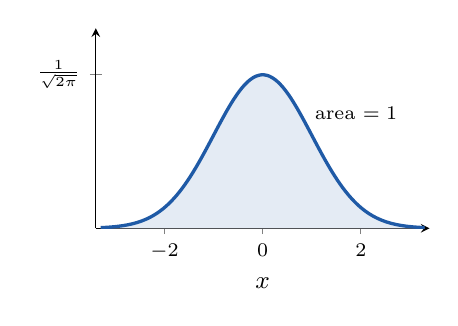
\begin{tikzpicture}
\begin{axis}[nfig, width=0.48\textwidth, height=0.34\textwidth,
  xmin=-3.4, xmax=3.4, ymin=0, ymax=0.52,
  xtick={-2,0,2}, ytick={0.3989}, yticklabels={$\tfrac{1}{\sqrt{2\pi}}$}, xlabel={$x$}]
  \addplot[draw=none, fill=figB!12, domain=-3.3:3.3, samples=120] {0.39894*exp(-x^2/2)} \closedcycle;
  \addplot[figB, very thick, domain=-3.3:3.3, samples=120] {0.39894*exp(-x^2/2)};
  \node[font=\scriptsize] at (axis cs:1.9,0.30) {area $=1$};
\end{axis}
\end{tikzpicture}\hfill
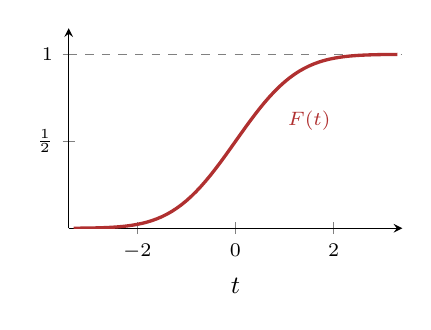
\begin{tikzpicture}
\begin{axis}[nfig, width=0.48\textwidth, height=0.34\textwidth,
  xmin=-3.4, xmax=3.4, ymin=0, ymax=1.15,
  xtick={-2,0,2}, ytick={0.5,1}, yticklabels={$\tfrac12$,$1$}, xlabel={$t$}]
  \addplot[black!50, dashed, thin] coordinates {(-3.4,1) (3.4,1)};
  \addplot[figR, very thick] coordinates {(-3.30,0.0005) (-3.20,0.0007) (-3.10,0.0010) (-3.00,0.0013) (-2.90,0.0019) (-2.80,0.0026) (-2.70,0.0035) (-2.60,0.0047) (-2.50,0.0062) (-2.40,0.0082) (-2.30,0.0107) (-2.20,0.0139) (-2.10,0.0179) (-2.00,0.0228) (-1.90,0.0287) (-1.80,0.0359) (-1.70,0.0446) (-1.60,0.0548) (-1.50,0.0668) (-1.40,0.0808) (-1.30,0.0968) (-1.20,0.1151) (-1.10,0.1357) (-1.00,0.1587) (-0.90,0.1841) (-0.80,0.2119) (-0.70,0.2420) (-0.60,0.2743) (-0.50,0.3085) (-0.40,0.3446) (-0.30,0.3821) (-0.20,0.4207) (-0.10,0.4602) (0.00,0.5000) (0.10,0.5398) (0.20,0.5793) (0.30,0.6179) (0.40,0.6554) (0.50,0.6915) (0.60,0.7257) (0.70,0.7580) (0.80,0.7881) (0.90,0.8159) (1.00,0.8413) (1.10,0.8643) (1.20,0.8849) (1.30,0.9032) (1.40,0.9192) (1.50,0.9332) (1.60,0.9452) (1.70,0.9554) (1.80,0.9641) (1.90,0.9713) (2.00,0.9772) (2.10,0.9821) (2.20,0.9861) (2.30,0.9893) (2.40,0.9918) (2.50,0.9938) (2.60,0.9953) (2.70,0.9965) (2.80,0.9974) (2.90,0.9981) (3.00,0.9987) (3.10,0.9990) (3.20,0.9993) (3.30,0.9995)};
  \node[font=\scriptsize, figR] at (axis cs:1.5,0.62) {$F(t)$};
\end{axis}
\end{tikzpicture}\figcap{The normal density $g$ (left; total area $1$) and its distribution function $F$ (right): the accumulated area climbs from $0$ to $1$, with $F(0) = \tfrac12$ by symmetry. By the remark above, $F' = g$ everywhere --- the sigmoid's slope at $t$ is the bell's height at $t$.}
\end{center}


\end{document}
